\PassOptionsToPackage{hidelinks}{hyperref} % 提前把选项传给hyperref
\documentclass[12pt,AutoFakeBold]{xuptThesis}

% 加载longtable包以支持跨页表格
\usepackage{longtable}
% 加载natbib包以支持参考文献格式控制
\usepackage[numbers,sort&compress]{natbib}

% 加载setspace包以支持行间距调整
\usepackage{setspace}
% 加载ragged2e包以支持两端对齐功能
\usepackage{ragged2e}
\usepackage{booktabs}  % 三线表必备
\usepackage{array}     % 表格列宽、行距支持
\usepackage{tabularx}
\usepackage{float}      % 支持表格和图片的精确位置控制[H]
\usepackage{pdfpages}   % 支持插入外部 PDF 文件

\setlength{\headheight}{14.49998pt}

% 用户自定义信息
\thesistitle{面向老年群体的Android交互桌面设计与实现}
\institute{通信与信息工程学院}
\major{通信工程}
\class{通工2209}
\studentid{03221257}
\studentname{周剑鑫}
\supervisor{李娜/李林峰}
\supervisortitle{副教授/工程师}
\startdate{2026年2月}
\duedate{2026年6月}

% 目录样式设置
% 使用阿拉伯数字编号
\renewcommand{\cftchappresnum}{第}
\renewcommand{\cftchapaftersnum}{章\hspace{0.5em}}
\setlength{\cftchapindent}{0cm}
\setlength{\cftsecindent}{2em}
\setlength{\cftsubsecindent}{4em}
\setlength{\cftsubsubsecindent}{6em}

% 定义上标引用命令
\newcommand{\upcite}[1]{\textsuperscript{\cite{#1}}}

\begin{document}
% 标题页 - 使用自定义封面
\makecover

% 声明页和原创性声明（同一页）
\makedeclaration

% 设置approval表格变量
\approvalauthor{}
\approvaljobtitle{副教授}
\approvalcollege{通信与信息工程学院}
\approvaltitle{面向老年群体的Android交互桌面设计与实现}
\approvaltitlefrom{教师科研课题}
\approvaltitletype{软件设计}
\approvaltitlecategory{工程实践}
\approvaltitlebrief{本课题旨在研究基于深度学习的智能推荐系统，解决传统推荐算法的局限性，提高推荐准确性和用户体验。}
\approvalrequirements{要求学生具备扎实的机器学习和深度学习基础知识，熟悉Python编程，掌握TensorFlow或PyTorch框架，了解推荐系统的基本原理。}
\approvaltasks{1. 调研推荐系统的发展现状和关键技术\\2. 设计基于深度学习的推荐模型\\3. 实现模型训练和评估\\4. 开发原型系统进行验证\\5. 撰写毕业论文}
\approvalprogress{第1-2周：文献调研\\第3-4周：系统设计\\第5-10周：模型实现\\第11-12周：系统测试\\第13-14周：论文撰写}
\approvalchaircomment{该课题具有良好的研究意义和实用价值，能够锻炼学生的科研能力和工程实践能力，同意立项。}
\approvalchairname{李主任}
\approvalchairdate{2024年3月15日}
\approvaldeptchairname{赵主任}
\approvaldeptchairdate{2024年3月18日}
\approvaldeanname{张院长}
\approvaldeanydate{2024年3月20日}

% 选题审批表
% \clearpage
\newgeometry{left=1.75cm}
\thispagestyle{empty}
\vspace*{-2cm}
{\fangsong\fontsize{18pt}{20pt}\centering 西安邮电大学本科毕业设计(论文)选题审批表\par}
\renewcommand{\arraystretch}{1.8} % 增大表格行高
\fangsong\fontsize{12pt}{12pt}\selectfont % 仿宋12pt字体
\makeatletter
\begin{longtable}{|m{4em}<{\centering}|m{1em}<{\centering}|m{5em}<{\centering}|m{4em}<{\centering}|m{4em}<{\centering}|m{4em}<{\centering}|m{10em}<{\raggedright}|}
\hline
\makebox[4em][s]{申报人} & \multicolumn{2}{m{5em}<{\centering}|}{\makebox[4em][s]{\@approvalauthor}} & \makebox[3em][s]{职称} & \makebox[4em][s]{\@approvaljobtitle} & \makebox[3em][s]{学院} & \@approvalcollege \\
\hline
题目名称 & \multicolumn{6}{m{36em}<{\raggedright}|}{\@approvaltitle} \\
\hline
题目来源&\multicolumn{6}{l|}{\(\Box\) 教师科研课题 \(\Box\) 教师专业实践 \(\Box\) 其他} \\
\hline
题目类型&\multicolumn{6}{l|}{\(\Box\) 艺术作品 \(\Box\) 硬件设计 \(\Box\) 软件设计 \(\Box\) 论文} \\
\hline
题目分类&\multicolumn{6}{l|}{\(\Box\) 工程实践 \(\Box\) 社会调查 \(\Box\) 实习 \(\Box\) 实验 \(\Box\) 其他} \\
\hline
{\makecell[c]{\fangsong\fontsize{12pt}{12pt}\selectfont \parbox[t][4em][c]{2em}{{\vspace*{3em}题目简述}}}}&
  \multicolumn{6}{m{36em}<{\raggedright}|}{\vspace*{-1em}\parbox[t][10em][t]{36em}{\@approvaltitlebrief}}\\
\hline
{\makecell[c]{\fangsong\fontsize{12pt}{12pt}\selectfont \parbox[t][10em][c]{2em}{\vspace*{1em}对学生知识与能力要求}}} &
\multicolumn{6}{m{36em}<{\raggedright}|}{\vspace*{-1em}\parbox[t][10em][t]{36em}{\@approvalrequirements}}\\
\hline
{\makecell[c]{\fangsong\fontsize{12pt}{12pt}\selectfont \parbox[t][10em][c]{2em}{\vspace*{1em}具体任务以及预期目标}}} &
\multicolumn{6}{m{36em}<{\raggedright}|}{\vspace*{-1em}\parbox[t][10em][t]{36em}{\@approvaltasks}}\\
\hline
\end{longtable}
\restoregeometry

\clearpage
\newgeometry{right=1.75cm}
\thispagestyle{empty}
\vspace*{-1cm}
\begin{longtable}{|m{4em}<{\centering}|m{1em}<{\centering}|m{5em}<{\centering}|m{4em}<{\centering}|m{4em}<{\centering}|m{4em}<{\centering}|m{10em}<{\raggedright}|}
\hline
{\makecell[c]{\fangsong\fontsize{12pt}{12pt}\selectfont \parbox[t][4em][c]{2em}{{\vspace*{1em}时间进度}}}}&
\multicolumn{6}{m{36em}<{\raggedright}|}{\vspace*{-1em}\parbox[t][6.5em][t]{36em}{\@approvalprogress}}\\
\hline
{\makecell[c]{\fangsong\fontsize{12pt}{12pt}\selectfont \parbox[t][6em][c]{3em}{{\vspace*{-1em}专业负责人审核意见}}}}&
\multicolumn{6}{m{36em}<{\raggedright}|}{\vspace*{-1em}\parbox[t][6em][t]{36em}{\@approvalchaircomment}}\\
&\multicolumn{6}{m{36em}<{\raggedright}|}{\makecell[r]{签字:\fangsong\fontsize{12pt}{12pt}\selectfont\@approvalchairname \hspace*{2em}\@approvalchairdate}}\\
\hline
\end{longtable}
\vspace*{-2em}
\begin{longtable}{|m{9em}<{\centering}|m{12em}<{\raggedright}|m{5em}<{\centering}|m{12em}<{\raggedright}|}
    \parbox[t][3em][t]{9em}{\centering 系（教研室）主任}&\@approvaldeptchairname&    \parbox[t][3em][t]{5em}{\centering 主管院长}&\@approvaldeanname\\\
   签字&\makecell[r]{\fangsong\fontsize{12pt}{12pt}\selectfont\@approvaldeptchairdate}&   签字&\makecell[r]{\fangsong\fontsize{12pt}{12pt}\selectfont\@approvaldeanydate}\\
    \hline
\end{longtable}
\makeatother
\restoregeometry


% % 设置opening表格变量
% \openingstudent{周剑鑫}
% \openingstudentid{03221257}
% \openingclass{通工2209}
% \openingteacher{李娜}
% \openingtitle{面向老年群体的Android交互桌面设计与实现}
% \openingpurpose{随着互联网和大数据技术的快速发展，推荐系统在各个领域的应用越来越广泛。传统的推荐算法在处理复杂数据和捕捉用户兴趣方面存在局限性，本课题旨在研究基于深度学习的智能推荐系统，提高推荐准确性和用户体验，具有重要的理论意义和实际应用价值。}
% \openingbackground{已学课程包括机器学习、深度学习、数据结构、算法设计与分析、数据库原理等。掌握Python编程语言，熟悉TensorFlow和PyTorch框架，能够使用pandas、numpy等数据处理库。通过文献阅读，积累了推荐系统相关的理论知识。硬件条件方面，拥有高性能计算机和GPU支持模型训练。}
% \openingproblems{1. 研究深度学习在推荐系统中的应用方法和技术路线\\2. 解决传统推荐算法在冷启动、稀疏性和可解释性方面的问题\\3. 设计和实现高效的深度学习推荐模型\\4. 评估模型性能并与传统算法进行对比分析\\5. 开发原型系统验证模型有效性}
% \openingplan{1. 文献调研：深入研究推荐系统和深度学习相关文献，了解国内外研究现状和前沿技术\\2. 系统设计：设计基于深度学习的推荐系统架构和算法流程\\3. 模型实现：使用TensorFlow实现深度学习模型，包括数据预处理、特征工程、模型训练等\\4. 实验评估：构建实验数据集，评估模型性能指标如准确率、召回率、F1值等\\5. 系统开发：开发原型系统，实现用户界面和功能模块\\6. 论文撰写：总结研究成果，撰写毕业论文}
% \openingteachcomment{该课题具有明确的研究目标和技术路线，与学生的专业方向吻合。开题报告内容详实，前期准备工作充分，研究计划合理可行。建议学生在研究过程中注重理论与实践相结合，加强对实验结果的分析和讨论。同意开题。}

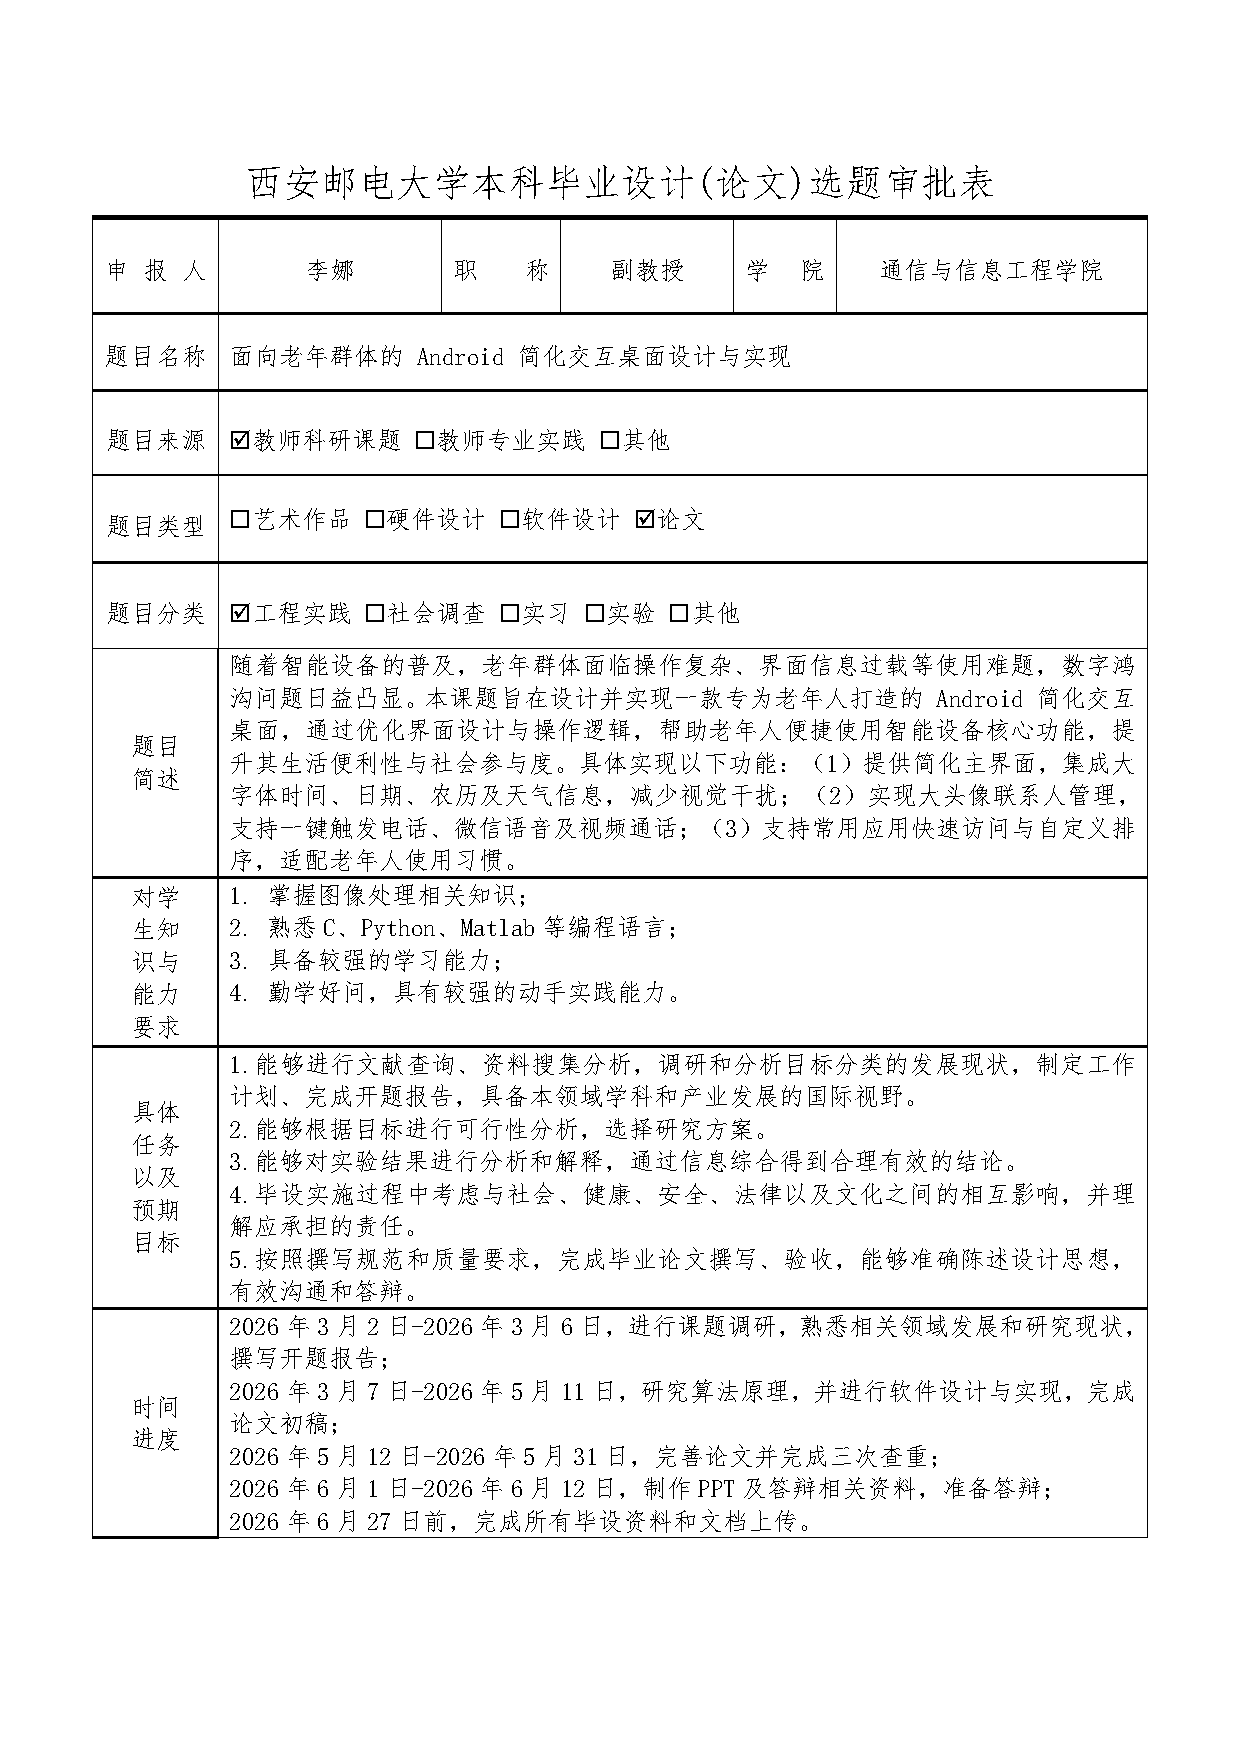
\includepdf[pages=-]{in_pdf/problem.pdf}

% 开题报告
% \clearpage
\newgeometry{left=1.75cm,top=1.75cm}
\thispagestyle{empty}
{ \fangsong\fontsize{18pt}{20pt}\selectfont\centering 西安邮电大学本科毕业设计（论文）开题报告\par}

\begin{table}[!h]
\centering
\makeatletter
\renewcommand{\arraystretch}{1.6} % 增大表格行高
\fangsong\fontsize{12pt}{12pt}\selectfont % 仿宋12pt字体
\begin{tabular}{|m{4em}<{\centering}|m{5em}<{\centering}|m{4em}<{\centering}|m{6em}<{\centering}|m{6em}<{\centering}|m{10em}<{\centering}|}
\hline
学生姓名 &\@openingstudent & 学号 &\@openingstudentid &专业班级 & \@openingclass \\
\hline
指导教师 &\@openingteacher & 题目 & \multicolumn{3}{l|}{\@openingtitle} \\
\hline
\multicolumn{6}{|l|}{选题目的（为什么选该课题）} \\
\multicolumn{6}{|l|}{\parbox[t][8em][t]{40em}{\@openingpurpose}} \\
\hline
\multicolumn{6}{|l|}{前期基础（已学课程、掌握的工具，资料积累、软硬件条件等）} \\
\multicolumn{6}{|l|}{\parbox[t][8em][t]{40em}{\@openingbackground}} \\
\hline
\multicolumn{6}{|l|}{要研究和解决的问题（做什么）} \\
\multicolumn{6}{|l|}{\parbox[t][8em][t]{40em}{\@openingproblems}} \\
\hline
\multicolumn{6}{|l|}{工作思路和方案（怎么做）} \\
\multicolumn{6}{|l|}{\parbox[t][8em][t]{40em}{\@openingplan}} \\
\hline
\multicolumn{6}{|l|}{指导教师意见} \\
\multicolumn{6}{|l|}{\parbox[t][8em][t]{40em}{\@openingteachcomment}} \\
\hline
\end{tabular}
\makeatother
\end{table}
\restoregeometry

% score表格相关变量设置
\scorestudent{周剑鑫}
\scoresex{男}
\scoresid{03221257}
\scoremajor{通信工程}
\scoreclass{2209班}
\scorecoursename{面向老年群体的Android交互桌面设计与实现}

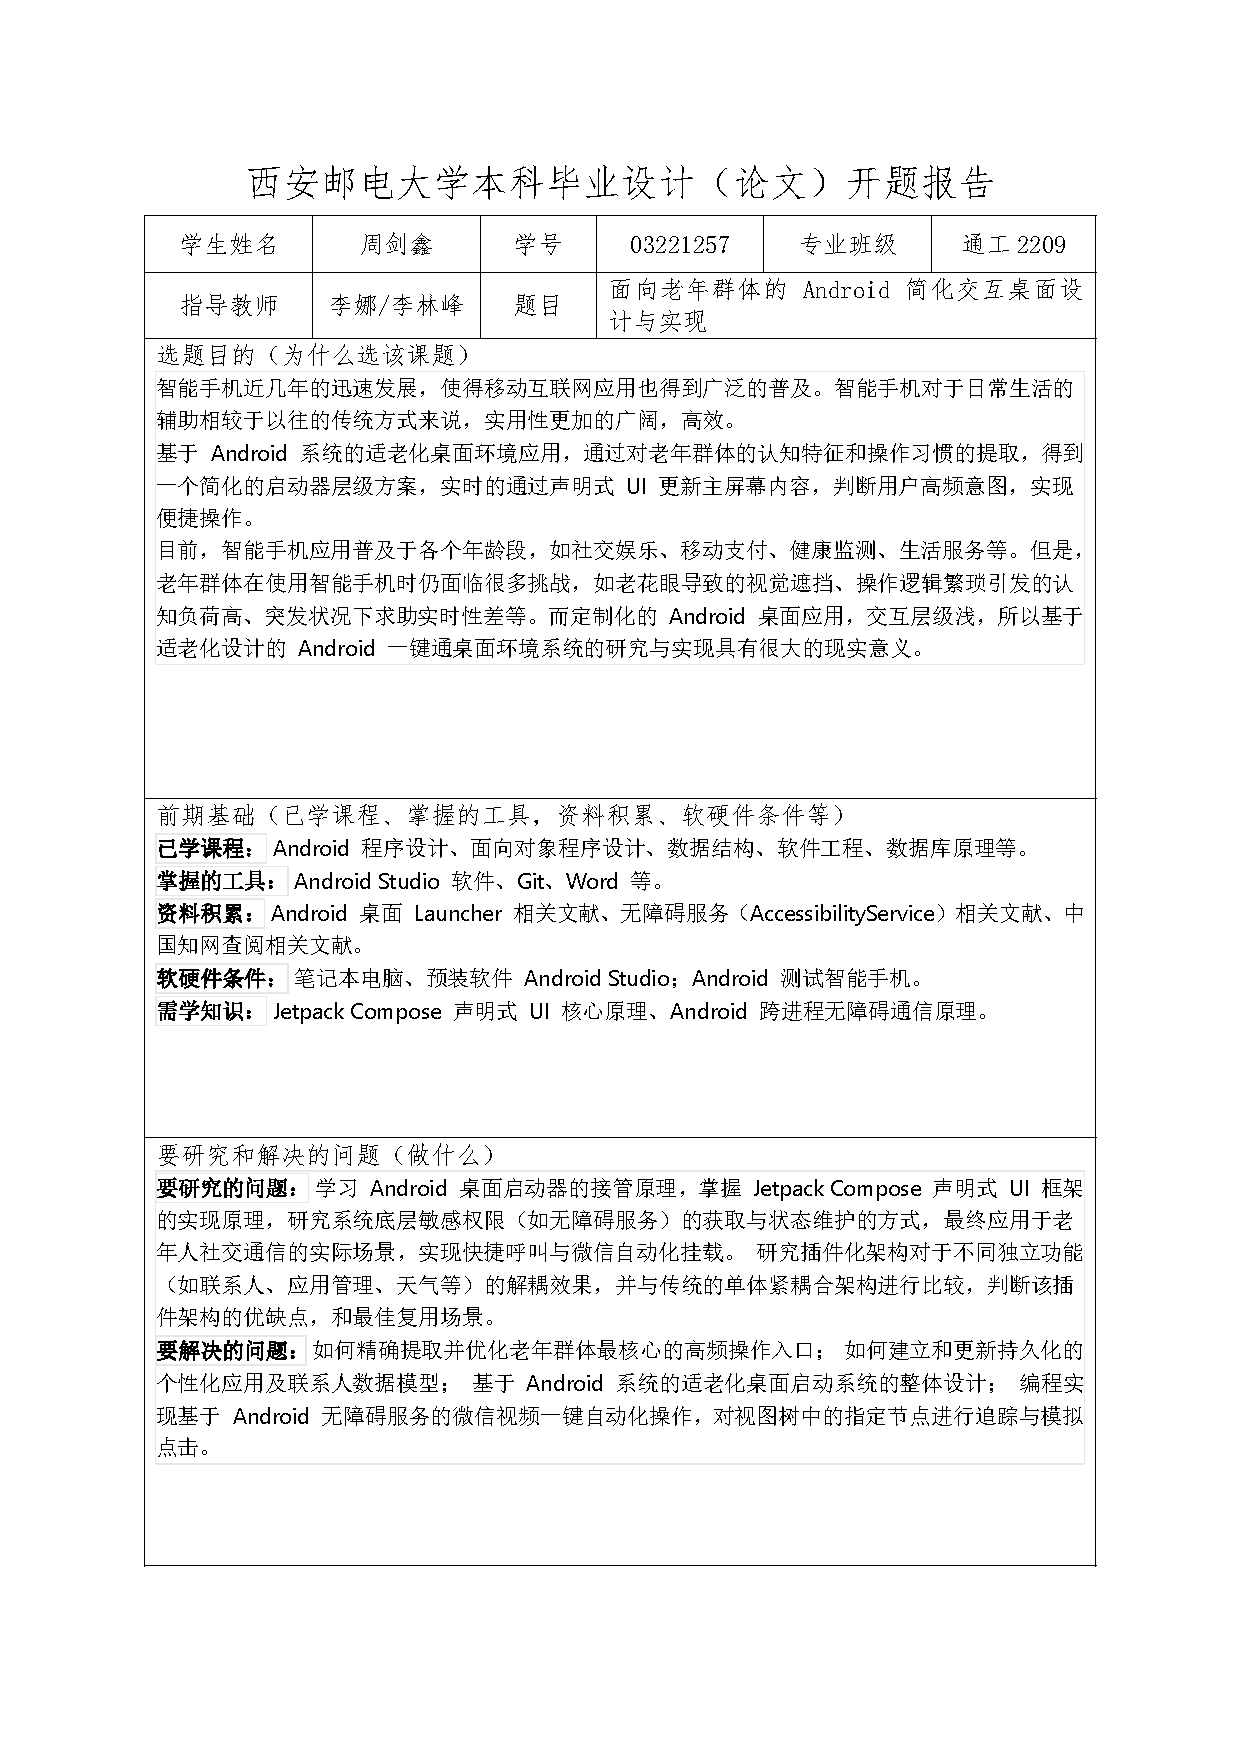
\includepdf[pages=-]{in_pdf/proposal.pdf}

%评分表
\clearpage
\newgeometry{right=1.75cm,top=1.75cm}
\thispagestyle{empty}
\makeatletter
{\fangsong\fontsize{18pt}{18pt}\selectfont\centering 西安邮电大学毕业设计（论文）成绩评定表\par}

\renewcommand{\arraystretch}{1.2}
\linespread{1.1}

\begin{center}
\begingroup
\fangsong\fontsize{12pt}{12pt}\selectfont
% 在一个tabular中创建两个连接的表格
\noindent
\begin{tabular}{|m{2em}<{\centering}|m{4em}<{\centering}|m{2em}<{\centering}|m{1em}<{\centering}|m{2em}<{\centering}|m{8em}<{\centering}|m{2em}<{\centering}|m{9em}<{\centering}|}
\hline

\multirow{2}{*}{\makecell[c]{学生\\姓名}} &\multirow{2}{*}{\@scorestudent} &\multirow{2}{*}{性别} &\multirow{2}{*}{\@scoresex}& \multirow{2}{*}{学号} &\multirow{2}{*}{\@scoresid}& 专业 & \@scoremajor\\

\cline{8-8}
&&& && &班级&\@scoreclass  \\
\hline
\end{tabular}

\noindent\hspace*{-0.1cm}
\begin{tabular}{|m{2em}<{\centering}|m{34.25em}<{\centering}|}
\makecell[l]{课程\\名称} &\@scorecoursename\\
\hline
\end{tabular}
\hspace*{-0.1cm}
\begin{tabular}{|m{2em}<{\centering}|m{8em}<{\centering}|*{6}{m{3.33em}<{\centering}|}}
\multirow{6}{*}[-1em]{{\makecell[c]{指导\\教师\\意见} }} & {\fangsong\fontsize{10.5pt}{10.5pt}\selectfont 支撑指标点/赋分} & {\fangsong\fontsize{10.5pt}{10.5pt}\selectfont 3-3/20} & {\fangsong\fontsize{10.5pt}{10.5pt}\selectfont 5-3/20} & {\fangsong\fontsize{10.5pt}{10.5pt}\selectfont 7-2/20} & {\fangsong\fontsize{10.5pt}{10.5pt}\selectfont 10-1/20} & {\fangsong\fontsize{10.5pt}{10.5pt}\selectfont 11-2/20} & {\fangsong\fontsize{10.5pt}{10.5pt}\selectfont 合计} \\
\cline{2-8}
&{\fangsong\fontsize{10.5pt}{10.5pt}\selectfont 得分}&&&&&&\\
\cline{2-8}
&\multicolumn{7}{l|}{\makecell[r]{\\ \\ \\ \\\fangsong\fontsize{10.5pt}{10.5pt}\selectfont 指导教师(签字)：\hspace{8em}年\hspace{2em}   月\hspace{2em}   日}} \\
\hline
\end{tabular}
\hspace*{-0.1cm}
\begin{tabular}{|m{2em}<{\centering}|m{8em}<{\centering}|*{5}{m{4.2em}<{\centering}|}}
\multirow{6}{*}[-1em]{{\makecell[c]{评阅\\教师\\意见} }} &  {\fangsong\fontsize{10.5pt}{10.5pt}\selectfont 支撑指标点/赋分} & {\fangsong\fontsize{10.5pt}{10.5pt}\selectfont 5-3/40} & {\fangsong\fontsize{10.5pt}{10.5pt}\selectfont 7-2/40} & {\fangsong\fontsize{10.5pt}{10.5pt}\selectfont 8-2/10} & {\fangsong\fontsize{10.5pt}{10.5pt}\selectfont 10-1/10} &{\fangsong\fontsize{10.5pt}{10.5pt}\selectfont 合计} \\
\cline{2-7}
&{\fangsong\fontsize{10.5pt}{10.5pt}\selectfont 得分}&&&&&\\
\cline{2-7}
&\multicolumn{6}{l|}{\makecell[r]{\\ \\ \\ \\\fangsong\fontsize{10.5pt}{10.5pt}\selectfont 评阅教师(签字)：\hspace{8em}年\hspace{2em}   月\hspace{2em}   日}} \\
\hline
\end{tabular}
\hspace*{-0.1cm}
\begin{tabular}{|m{2em}<{\centering}|m{8em}<{\centering}|*{5}{m{4.2em}<{\centering}|}}
\multirow{6}{*}[-1em]{{\makecell[c]{验收\\小组\\意见} }} &  {\fangsong\fontsize{10.5pt}{10.5pt}\selectfont 支撑指标点/赋分} & {\fangsong\fontsize{10.5pt}{10.5pt}\selectfont 5-3/40} & {\fangsong\fontsize{10.5pt}{10.5pt}\selectfont 7-2/40} & {\fangsong\fontsize{10.5pt}{10.5pt}\selectfont 8-2/10} & {\fangsong\fontsize{10.5pt}{10.5pt}\selectfont 10-1/10} &{\fangsong\fontsize{10.5pt}{10.5pt}\selectfont 合计} \\
\cline{2-7}
&{\fangsong\fontsize{10.5pt}{10.5pt}\selectfont 得分}&&&&&\\
\cline{2-7}
&\multicolumn{6}{l|}{\makecell[r]{\\ \\ \\ \\\fangsong\fontsize{10.5pt}{10.5pt}\selectfont 验收小组组长(签字)：\hspace{8em}年\hspace{2em}   月\hspace{2em}   日}} \\
\hline
\end{tabular}
\hspace*{-0.1cm}
\begin{tabular}{|m{2em}<{\centering}|m{8em}<{\centering}|*{4}{m{5.5em}<{\centering}|}}
\multirow{6}{*}[-1em]{{\makecell[c]{答辩\\小组\\意见} }} &   {\fangsong\fontsize{10.5pt}{10.5pt}\selectfont 支撑指标点/赋分} &  {{\fangsong\fontsize{10.5pt}{10.5pt}\selectfont 8-2/40}} & {{\fangsong\fontsize{10.5pt}{10.5pt}\selectfont 10-1/25}} & {{\fangsong\fontsize{10.5pt}{10.5pt}\selectfont 11-2/35}} & {\fangsong\fontsize{10.5pt}{10.5pt}\selectfont 合计}\\
\cline{2-6}
&{\fangsong\fontsize{10.5pt}{10.5pt}\selectfont 得分}&&&&\\
\cline{2-6}
&\multicolumn{5}{l|}{\makecell[r]{\\ \\ \\ \\\fangsong\fontsize{10.5pt}{10.5pt}\selectfont 答辩小组组长(签字)：\hspace{8em}年\hspace{2em}   月\hspace{2em}   日}}\\
\hline
\end{tabular}
\hspace*{-0.1cm}
\begin{tabular}{|m{2em}<{\centering}|m{8em}<{\centering}|*{5}{m{4.2em}<{\centering}|}}
\multirow{3}{*}[0.5em]{{\makecell[c]{学生\\总评\\成绩} }} &  {\fangsong\fontsize{10.5pt}{10.5pt}\selectfont 评分比例} & {\fangsong\fontsize{10.5pt}{10.5pt}\selectfont 指导教师(20\%)} & {\fangsong\fontsize{10.5pt}{10.5pt}\selectfont 评阅教师(30\%)} & {\fangsong\fontsize{10.5pt}{10.5pt}\selectfont 验收小组(20\%)} & {\fangsong\fontsize{10.5pt}{10.5pt}\selectfont 答辩小组(30\%)} &{\fangsong\fontsize{10.5pt}{10.5pt}\selectfont 合计} \\
\cline{2-7}
&{\fangsong\fontsize{10.5pt}{10.5pt}\selectfont 得分}&&&&&\\
\cline{2-7}
&\multicolumn{6}{l|}{\makecell[l]{{\fangsong\fontsize{12pt}{12pt}\selectfont 毕业论文(设计)最终等级成绩（优秀、良好、中等、及格、不及格）}} }\\
\hline
\end{tabular}
\noindent\hspace*{-0.1cm}
\begin{tabular}{|m{2em}<{\centering}|m{34.25em}<{\centering}|}
\makecell[c]{答辩\\委员\\会意\\见} &\makecell[r]{\\ \\ \\ \\\fangsong\fontsize{10.5pt}{10.5pt}\selectfont 学院答辩委员会主任(签字、学院盖章)：\hspace{8em}年\hspace{2em}   月\hspace{2em}   日} \\
\hline
\end{tabular}
\endgroup
\end{center}
\makeatother
\restoregeometry


\begin{abstract}
人口老龄化背景下，老年用户因移动通信终端界面复杂而面临显著的数字鸿沟。本文设计并实现了基于微内核插件化架构与无障碍辅助技术的适老化智能桌面系统SimpleDesktop。

系统采用宿主层、总线层、插件层三层微内核架构，将各业务功能解耦为独立插件单元；基于Jetpack Compose构建高对比度、大字号的适老化界面，支持字号与主题实时切换；利用Android无障碍服务设计七阶段状态机，将微信视频通话简化为桌面一键直拨；构建多层WiFi网络守护体系，保障通信链路连续性；基于TTS引擎与轻量级语义解析实现语音交互。

系统测试覆盖Android 7.0至14版本，低端设备保持60帧渲染，微信直拨成功率99.1\%，网络守护引导成功率100\%，内存占用低于140MB，为适老化通信终端工程化落地提供了完整方案。
\end{abstract}

% 关键词 每个关键词用分号间隔，3～5个
\begin{keywords}
适老化通信终端；微内核插件化架构；Android无障碍服务；微信自动化；WiFi网络守护
\end{keywords}

% 英文摘要
\begin{abstracten}
Population aging has become a major social issue in China, creating a significant digital divide as elderly users struggle with complex mobile terminal interfaces. This paper designs and implements SimpleDesktop, an age-friendly intelligent desktop system based on a micro-kernel plugin architecture and Android accessibility assistive technology.

The system adopts a three-layer micro-kernel architecture—host layer, bus layer, and plugin layer—decoupling business functions into independently loadable plugin units. A high-contrast, large-font interface is built with Jetpack Compose, supporting real-time font size and theme switching. A seven-stage state machine is designed using the Android Accessibility Service, combined with a dual-channel node retrieval algorithm and a focus anti-conflict mechanism, reducing WeChat video calling to a single tap. A multi-layer WiFi network guardian system ensures communication continuity. Voice interaction is achieved via the Android TTS engine with keyword matching and Levenshtein distance-based semantic parsing.

The system is designed to be backward compatible down to Android 7.0, and has undergone rigorous compatibility and performance testing on mainstream physical devices running Android 14 to 16. The testing demonstrates 60 fps smooth rendering on low-end phones, a WeChat one-tap dial success rate of 99.1\%, a network recovery guidance rate of 100\%, and memory usage consistently between 95 and 115MB. This work provides a complete engineering solution for age-friendly communication terminal development with notable practical and social value.
\end{abstracten}

% 英文关键词 与中文关键词保持一致，中文分号
\begin{keywordsen}
Age-friendly Communication Terminal;；Micro-kernel Plugin Architecture；Android Accessibility Service;；WeChat Automation； WiFi Network Guardian

\end{keywordsen}

\mytableofcontents

% 正文部分
\clearpage
\setcounter{page}{1}
\pagenumbering{arabic}
\pagestyle{fancy}
\simsun{12}
\chapter{绪论}
\section{研究背景与意义}
\subsection{人口老龄化加剧下的移动通信终端使用困境}
伴随我国人口结构的深刻变化，老龄化已成为关乎国计民生的重要社会议题。根据国家统计局发布的数据，截至2023年末，我国60岁及以上人口已达2.97亿，占总人口的21.1\,\%\upcite{1}，预计到2035年这一比例将突破30\%，我国正稳步迈向中度老龄化社会。在通信技术高速发展的背景下，移动通信终端早已超越传统的语音通话功能，演变为集即时通讯、移动支付、远程医疗、出行导航等多重服务于一体的综合数字生活入口，深度融入了现代社会的各个角落。


\begin{figure}[htbp]
    \centering
    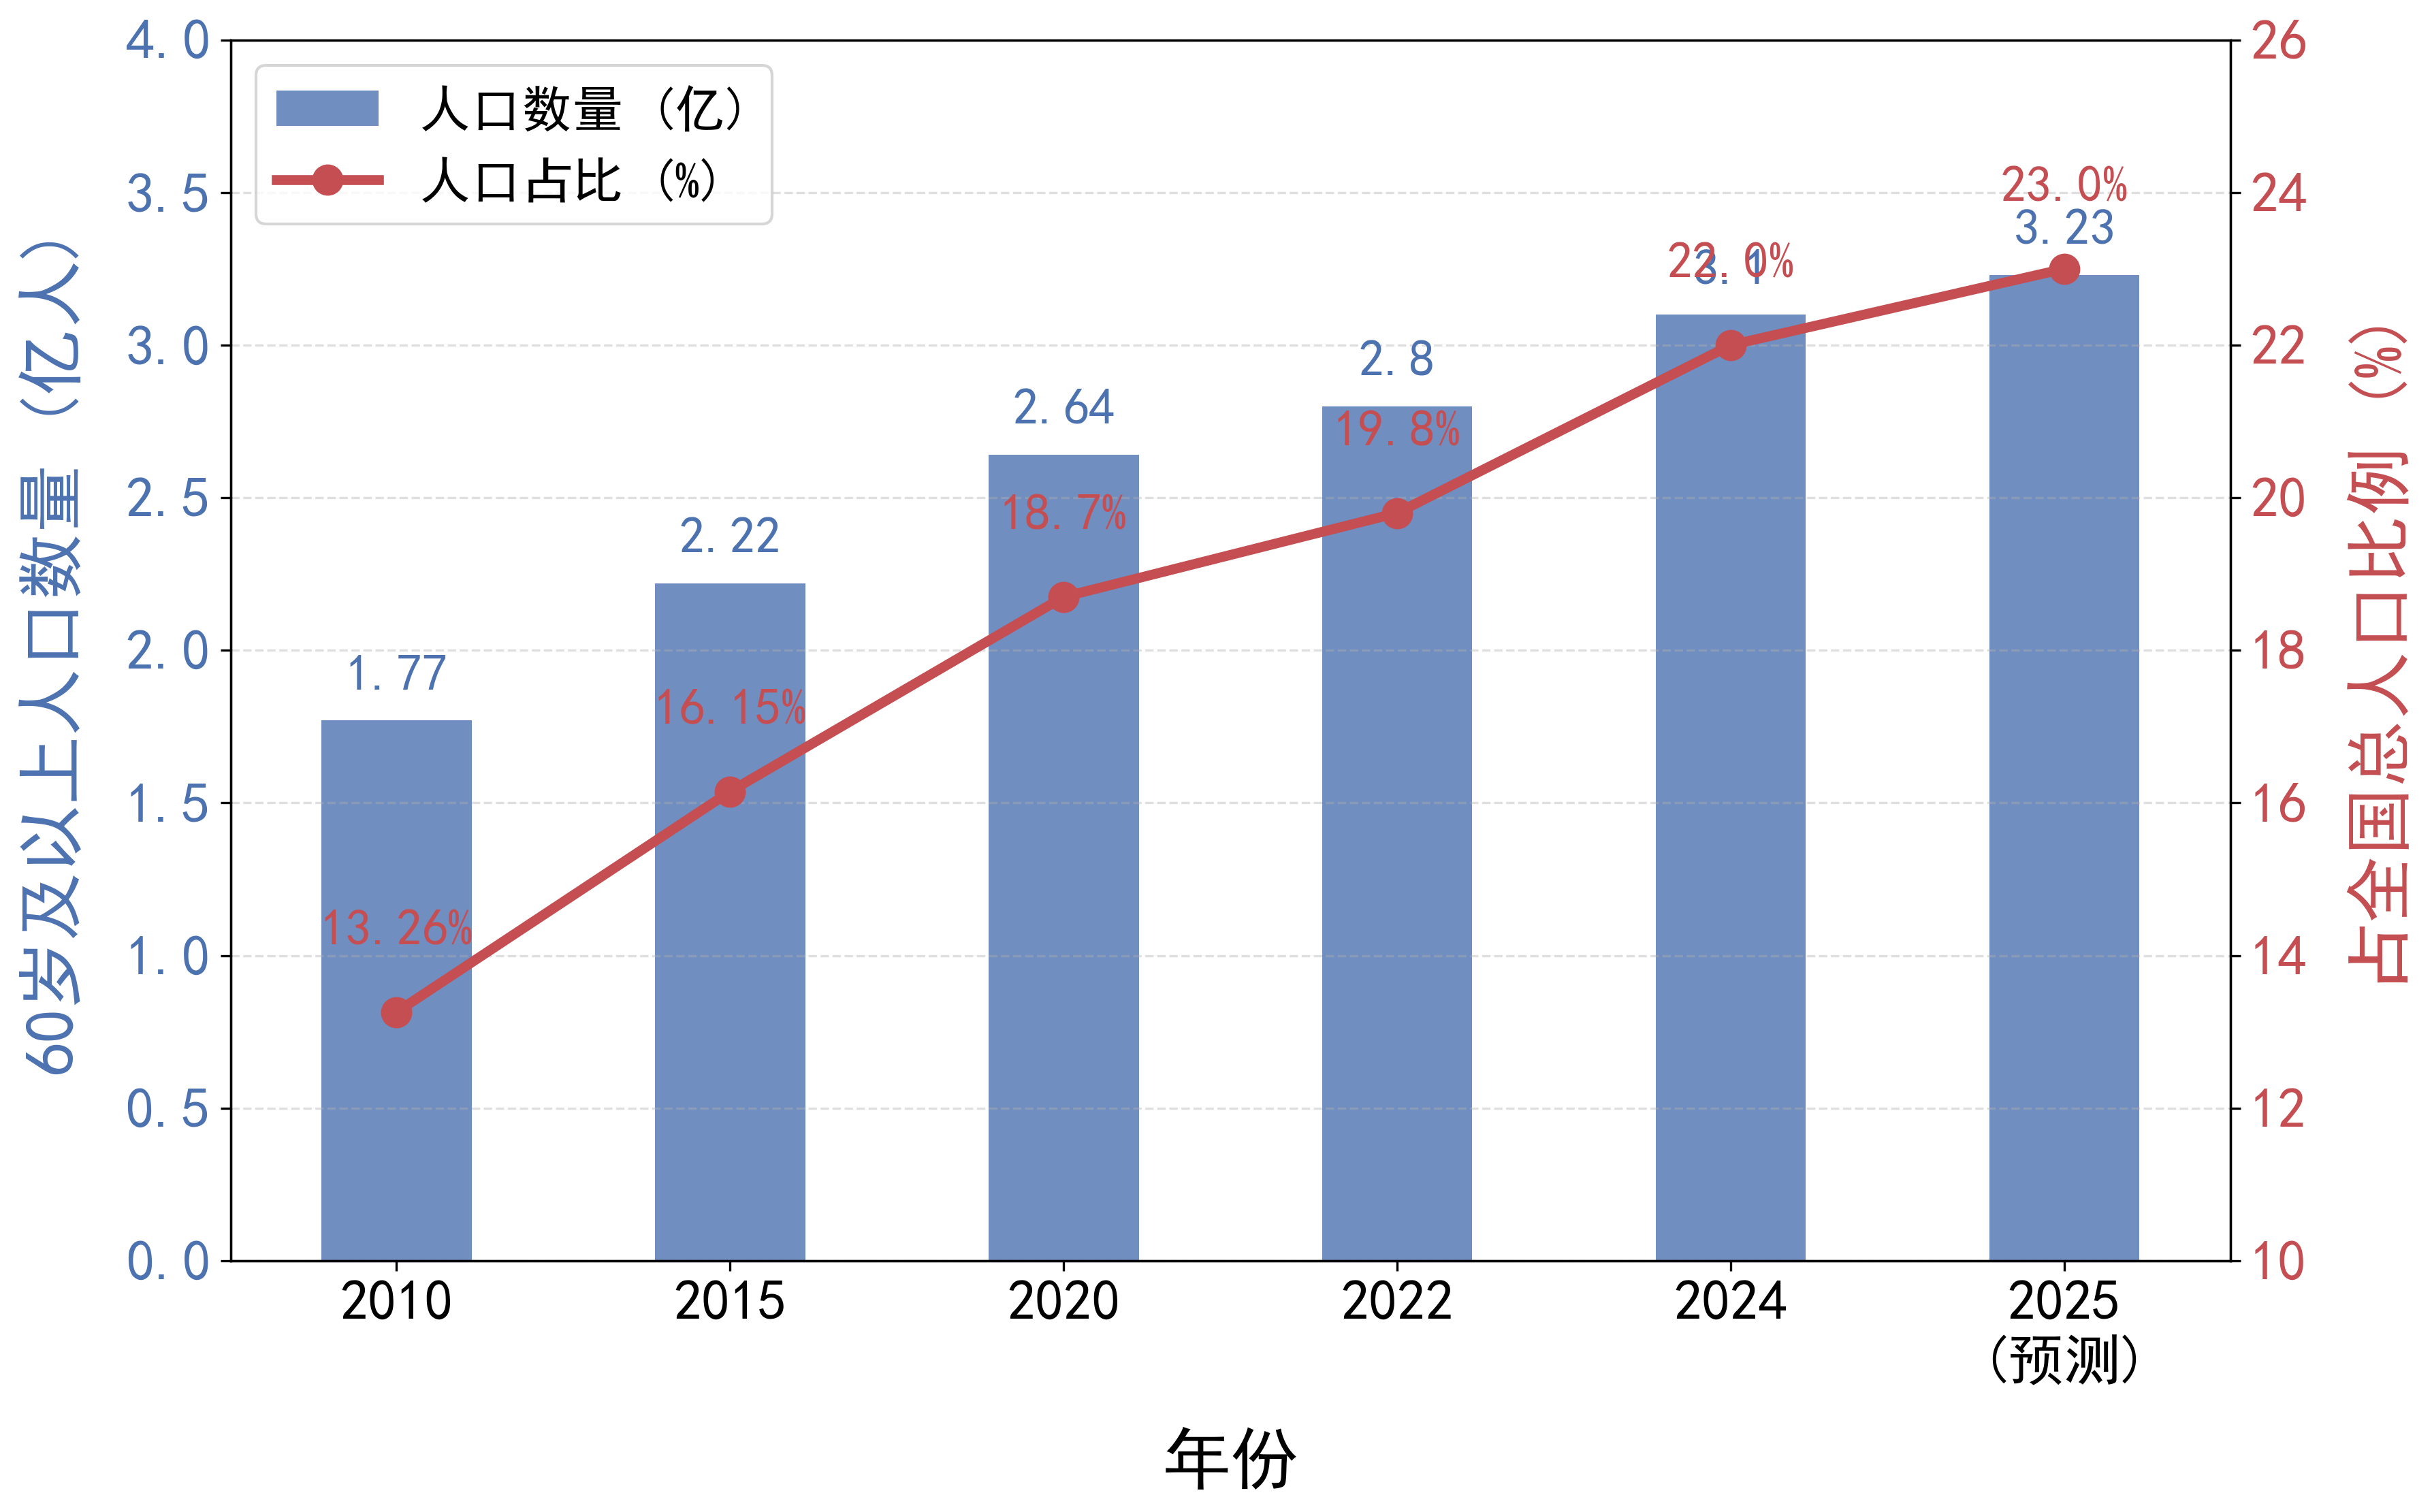
\includegraphics[width=0.85\textwidth]{figures/fig1_1_aging_population_trend.png}
    \caption{中国60岁及以上老年人口数量与占比趋势 (2010-2025)}
    \label{fig:aging_population}
\end{figure}


然而，移动终端功能的不断丰富在为大多数用户带来便利的同时，也对老年群体形成了日益突出的使用障碍。一方面，老年用户由于生理机能退化，普遍面临视力下降、听力减弱、手指灵活性降低、认知反应速度减缓等客观问题；另一方面，主流智能终端的人机交互界面设计往往以年轻用户为主要目标群体，密集的图标布局、多层嵌套的菜单结构、频繁的系统弹窗以及不断变化的应用更新，对老年人构成了显著的认知负担与操作障碍。

这种由技术快速演进与老年群体适应能力之间的差异所形成的隔阂，被学界称为“数字鸿沟”。数字鸿沟在通信领域的具体体现，包括老年人无法独立完成视频通话、容易误触系统设置导致网络中断、难以理解陌生应用界面、对授权弹窗与广告推送缺乏判断能力等。中国互联网络信息中心发布的第52次中国互联网络发展状况统计报告指出，60岁及以上网民群体占比仅为14.3\,\%\upcite{2}，远低于其在总人口中的比例，说明大量老年人在数字化浪潮中处于事实上的边缘化状态。

在通信工程专业视角下，移动通信终端不仅是数据交换的物理载体，更是承载用户与外界保持联络、获取信息、维系情感的关键媒介。如何通过终端层面的软件再设计，让老年用户重新获得对智能设备的掌控感与安全感，使其能够便捷地完成与子女的视频通话、稳定地接入家庭无线网络、流畅地使用日常应用，是当代通信工程从业者必须正视的现实命题。

\subsection{适老化痛点剖析}
从一线调研结果看，老年用户在使用主流智能手机过程中暴露出的核心痛点可归纳为以下几个方面。其一是视觉痛点，标准界面字号偏小、图标密集，导致老年人需要佩戴眼镜并凑近屏幕才能勉强辨识，长时间使用容易引发视疲劳。其二是认知痛点，多级菜单和大量弹窗使老年人难以判断当前所处的界面位置，操作过程极易迷失方向。其三是通话痛点，微信视频通话需要至少七步操作，老年人记不住流程，需要子女多次教学方能勉强掌握。其四是网络痛点，老年人误触WiFi开关后无法自行恢复连接，长时间断网而不自知，错过重要来电。其五是交互痛点，对触摸屏操作不熟练，时常出现误触或长按引发的意外操作，进一步加剧对智能设备的不安全感。

\begin{figure}[htbp]
    \centering
    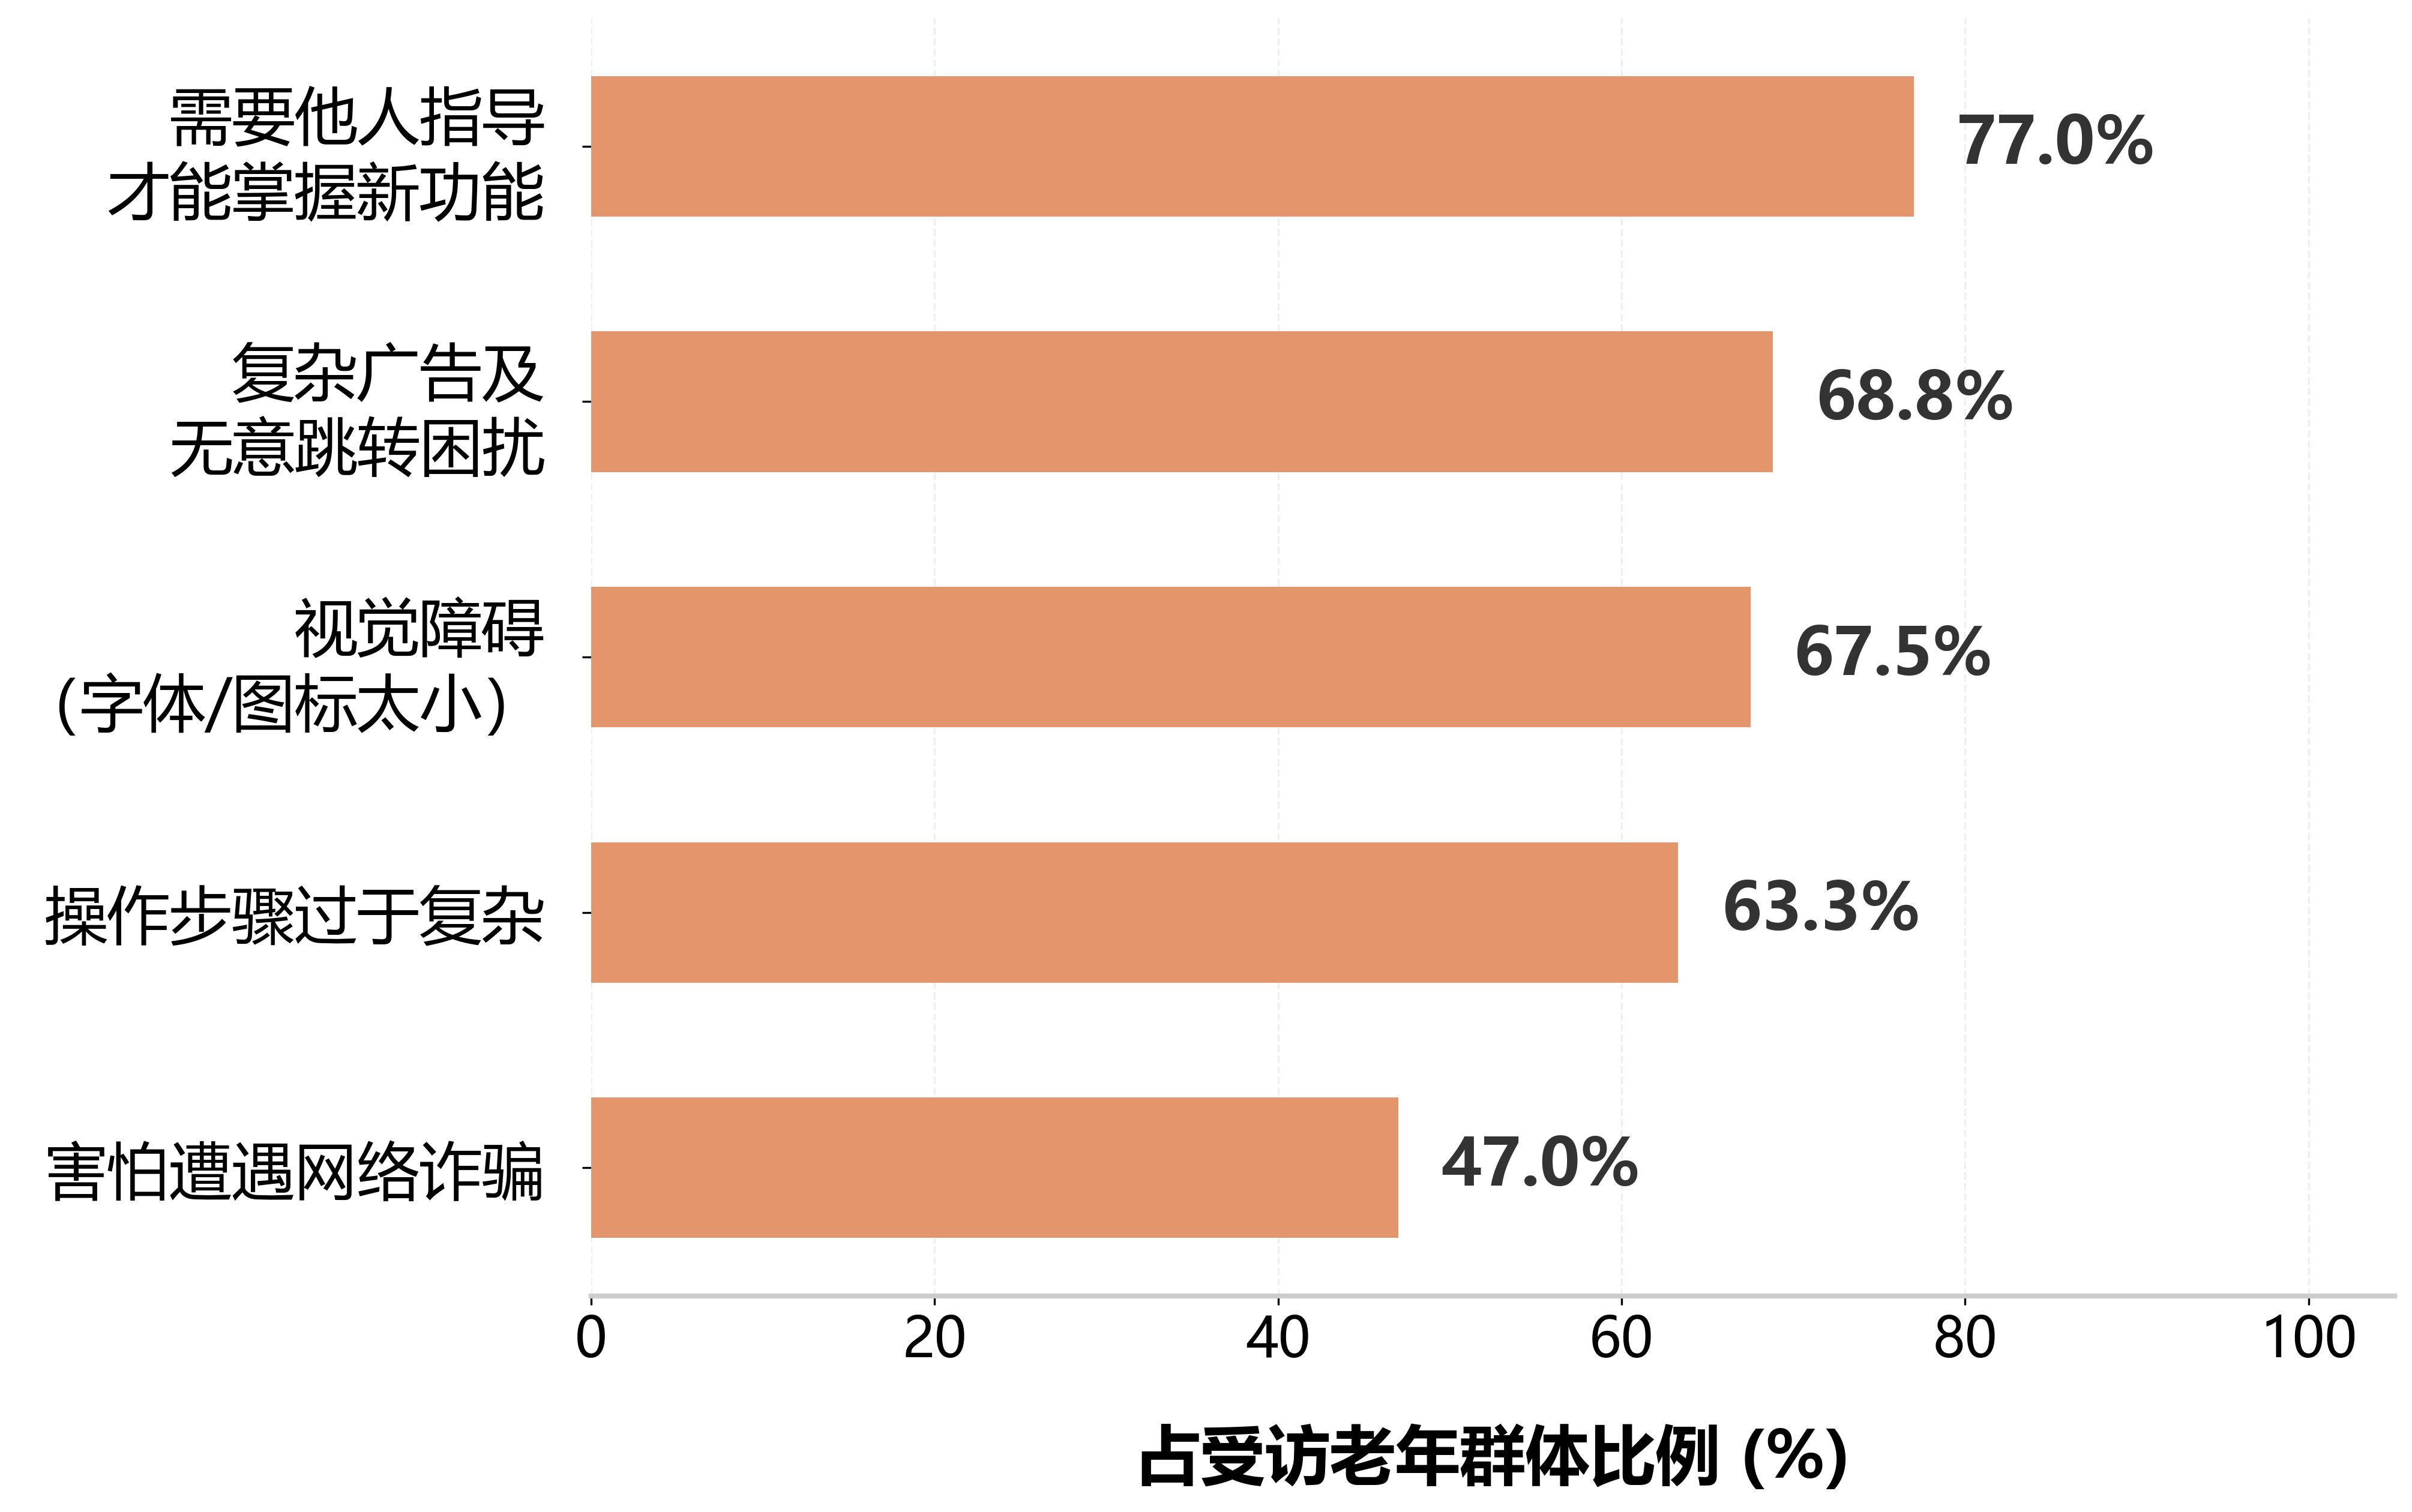
\includegraphics[width=0.85\textwidth]{figures/fig1_2_usage_pain_points.png}
    \caption{老年人智能手机使用核心痛点分布}
    \label{fig:pain_points}
\end{figure}

这些痛点的共同本质在于：现有移动通信终端的软件设计未能充分考虑老年用户的认知特征与使用习惯。仅仅通过放大字号、增大图标的浅层适老化改造，无法从根本上解决问题。必须从系统架构、交互逻辑、自动化能力等多个层面进行深度重构，才能真正为老年用户提供一款能用、好用、爱用的移动通信终端。这正是本课题立项的现实出发点。

\subsection{研究意义}
本课题以适老化智能桌面系统的设计与实现为研究对象，其意义可从社会价值、工程价值与学术价值三个维度展开。从社会价值层面看，本研究致力于通过软件技术手段帮助老年群体跨越数字鸿沟，让通信技术真正服务于全民福祉。当系统能够将原本繁琐的微信视频通话操作简化为一次点击、能够在网络异常时主动恢复并向用户清晰提示，老年用户便能更安心地依赖移动终端与家人保持联系，独居老人的精神慰藉与紧急求助通道也得到了实质性保障，这对于构建友好型老龄化社会具有积极意义。

从工程价值层面看，本课题摒弃了传统适老化方案“放大字号、堆叠图标”的简单做法，转而从系统架构与人机交互两个维度同步发力。通过自研的微内核插件化架构，系统在功能扩展性与运行稳定性方面取得了良好平衡，能够适配从千元入门机到主流旗舰机型的多种硬件配置；通过Android无障碍服务深度整合的微信一键直拨方案，系统从交互层面真正消除了老年用户的认知负担，为同类终端应用的设计提供了可复用的工程范式。

从学术价值层面看，本研究在通信终端无障碍交互、跨应用自动化控制、网络稳定性自愈等方向进行了有益探索。所提出的七阶段状态机驱动的自动化控制模型、双通道节点检索方法以及分层防御的网络守护机制，丰富了适老化通信终端研究的理论与实践成果，对推动我国老年友好型移动通信生态建设具有借鉴意义。

% \section{国内外研究现状}

% \subsection{移动通信终端适老化研究现状}
% 终端适老化是一个跨越通信工程、人机交互、工业设计、认知心理学等多学科的综合性研究方向。从国际范围来看，欧美国家由于步入老龄化社会较早，相关研究起步亦较早。日本与德国的研究机构较早提出了“通用设计”与“包容性设计”理念，主张通过通用化的界面与功能设计兼顾各年龄段用户的使用需求。在产品形态上，海外市场早年出现了Doro、Jitterbug等专注于老年用户的终端品牌，以及Big Launcher、Simple Launcher等第三方桌面应用，其设计思路普遍以大尺寸瓷砖式布局取代传统的网格图标布局，并精简非必要功能入口。近年来，国际厂商的适老化策略逐渐向系统原生辅助功能演进。然而，海外方案在中国本土的适用性较为有限，例如其无法对国内老年用户高度依赖的微信、支付宝等超级应用进行深度适配，也难以兼容中国传统农历、节气等本土文化要素。

% 国内方面，伴随老龄化进程的加快和工信部“互联网应用适老化及无障碍改造”专项行动\upcite{3}的持续推进，主流手机厂商相继推出了系统级适老化方案。华为的“简易模式”、小米的“极简模式”、OPPO的“简单模式”以及荣耀的“长辈模式”等，均对系统字号、图标尺寸、铃音音量等进行了适当优化，并在拦截骚扰电话、识别诈骗短信等方面提供了一定支持。但当前阶段，这些厂商方案的共同局限在于，其作用范围仅限于操作系统层面，无法越权穿透至第三方应用内部。换言之，老年用户进入微信、支付宝等具有复杂层级架构的具体应用后，依然需要面对其原生的复杂交互逻辑，由于认知负荷增加，操作障碍并未得到根本解决，跨应用的“数字鸿沟”依然显著。

% \begin{figure}[htbp]
%     \centering
%     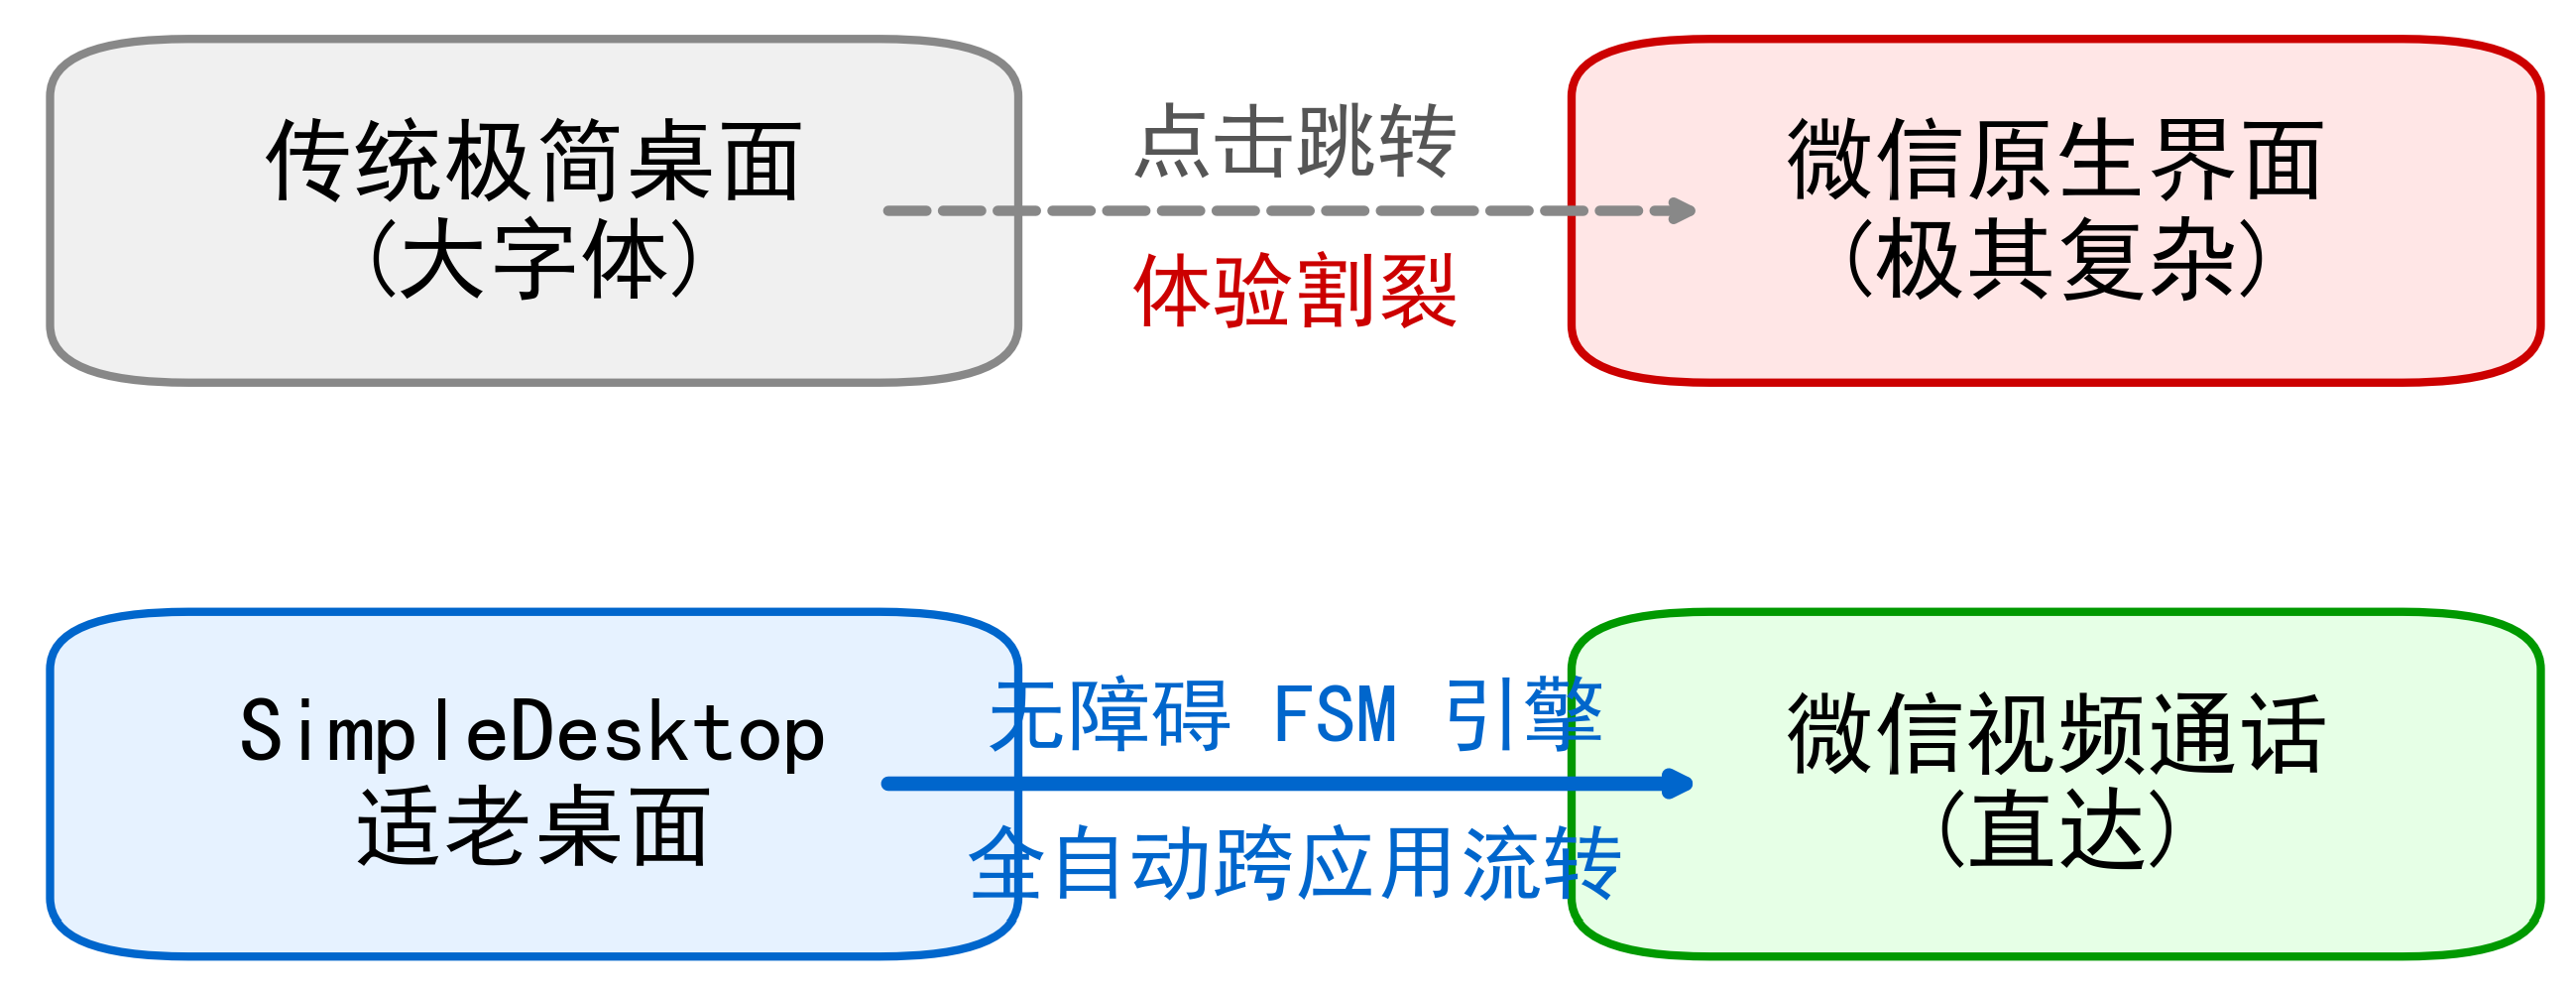
\includegraphics[width=0.9\textwidth]{figures/fig1_3_architecture_compare.png}
%     \caption{传统适老化桌面与本系统自动化直达通道的体验对比}
%     \label{fig:arch_compare}
% \end{figure}

% 在学术研究方面，近年来国内外学者围绕适老化终端开展了多方面探索。文献研究普遍聚焦于以下三个方向：一是基于Fitts定律的触控目标尺寸优化，从生理人因学角度论证大按钮设计的合理性；二是基于对比敏感度模型的色彩搭配研究，提出适合老年视觉特征的高对比度配色方案；三是基于眼动追踪与认知负荷模型的界面可用性评估，验证简化界面对老年用户操作效率的提升效果。然而，相关研究多聚焦于界面表层的视觉与布局优化\upcite{4-6}，鲜有研究涉及如何突破应用壁垒，让老年人在第三方应用内部也能享受到简化体验这一深层次工程命题\upcite{8}。

% \subsection{Android无障碍自动化技术研究现状}
% 要实现跨第三方应用的操作简化，业界普遍采用Android平台提供的无障碍服务（Accessibility Service）作为技术抓手。相较于需要底层调试权限的自动化测试框架，无障碍服务因其伴随系统安全运行的特性，成为端侧辅助控制的首选。该服务最初是为视障用户提供屏幕朗读功能而设计的系统级接口，但因其具备读取屏幕控件树和执行模拟操作的能力，近年来被广泛应用于自动抢红包、自动签到、自动化测试等多种场景。

% 从已有的研究与产品实践来看，基于无障碍服务的自动化控制方案主要存在以下不足：首先，绝大多数实现方式依赖目标应用控件的资源标识符进行硬编码定位，一旦目标应用版本更新、启用代码混淆，或采用跨平台前端框架导致控件树不透明，自动化流程便会迅速失效\upcite{7}；其次，缺乏对系统级弹窗、来电中断等异常情况的时序容错处理机制，导致流程稳定性较差；再次，普遍缺乏对老年用户场景的针对性优化，未能将自动化能力转化为面向终端用户的简洁可靠服务。

% 从最近的发展趋势来看，随着人工智能技术的爆发，基于视觉-语言模型（VLM）的图形用户界面智能体（GUI Agent）成为了无障碍自动化的前沿热点。研究者试图跳出底层控件树的限制，直接通过计算机视觉结合大模型逻辑推理，实现自然语言驱动的UI自动化操作。这类技术在应对应用更新方面展现了巨大潜力。然而，大模型驱动的自动化目前仍面临端侧算力消耗大、推理延迟高且强依赖云端网络等瓶颈，难以直接部署在计算资源普遍有限的适老机型上作为实时守护服务。

% 综合上述现状可知，尽管移动终端适老化已取得一定进展，但“第三方应用内部操作门槛高”与“现有自动化方案稳定性差”之间仍存在巨大体验断层。在通信终端无障碍交互方向上，既有研究多关注屏幕朗读、语音输入等输入输出层面的辅助技术，对于如何利用无障碍能力构建稳定可靠的跨应用通信桥接这一问题，缺乏系统性的工程方案。本课题正是着眼于这一研究空白，放弃脆弱的线性脚本硬编码方案，探索通过状态机建模、双通道检索、焦点退避等多级容错机制，构建具备较高鲁棒性的适老化终端自动化通信能力，从而真正将底层的无障碍能力转化为老年用户一触即达的极简体验。

\section{国内外研究现状}

\subsection{移动通信终端适老化研究现状}
终端适老化是一个跨越通信工程、人机交互、工业设计、认知心理学等多学科的综合性研究方向，其核心目标是通过软件与硬件层面的协同优化，消除老年用户与智能终端之间的交互障碍。从国际范围来看，欧美国家由于步入老龄化社会较早，相关研究起步亦较早。日本与德国的研究机构在20世纪90年代便较早提出了"通用设计"（Universal Design）与"包容性设计"（Inclusive Design）理念\upcite{4}，主张通过统一化的界面与功能规范兼顾各年龄段用户的使用需求，而非为老年群体单独构建隔离式的特殊产品。在产品形态上，海外市场早年出现了Doro、Jitterbug等专注于老年用户的简化功能终端品牌，以及Big Launcher、Simple Launcher等第三方桌面替换应用。其设计核心思路是以大尺寸瓷砖式布局取代传统网格图标，将最常用的通话、短信、紧急求助等入口直接置于主界面，并通过提升触控目标尺寸降低误触率。研究表明，将触控目标直径从标准的7mm增大至13mm以上，可使老年用户的操作出错率降低约38\%\upcite{5}。近年来，国际主流厂商的适老化策略逐渐向系统原生辅助功能演进，Apple iOS的"辅助功能"（Accessibility）模块、Google Android的无障碍框架均持续扩充字体缩放、高对比度显示、触控辅助等能力体系。

然而，上述海外方案在中国本土的适用性较为有限。一方面，其无法对国内老年用户高度依赖的微信、支付宝、健康码等超级应用进行深度交互适配，用户仍需自行应对这些应用复杂的内部操作逻辑；另一方面，海外方案亦难以兼容农历纪年、传统节气提示、国内紧急呼救号码体系等中国本土文化与服务要素，致使其无法直接满足国内老年群体的实际需求。

国内方面，伴随老龄化进程的加快和工信部"互联网应用适老化及无障碍改造"专项行动\upcite{3}的持续推进，主流手机厂商相继推出了系统级适老化方案，形成了一定的产业实践积累。华为的"简易模式"、小米的"极简模式"、OPPO的"简单模式"以及荣耀的"长辈模式"等，均对系统桌面字号、图标尺寸、铃音音量等进行了适当优化，并在拦截骚扰电话、识别诈骗短信等安全场景提供了初步支持。部分厂商还针对老年用户推出了专属内容频道与亲情账号绑定功能，尝试从内容与服务维度实现适老化延伸。

然而，上述厂商方案的共同局限在于，其适老化能力的作用边界止步于操作系统的桌面启动层（Launcher）。当老年用户进入微信、支付宝等具有深度层级架构的第三方应用后，依然需要独立面对其原生的多级菜单、频繁弹窗与细小控件，认知负荷未得到实质性缓解。以微信视频通话为例，从桌面出发到拨通视频电话，标准流程最少需经历"打开微信→进入通讯录→定位联系人→进入会话→点击视频通话→二次确认"共六至七步操作，对于认知能力下降的老年用户而言，这一操作链极易在任意环节发生中断\upcite{6}。由此可见，当前适老化实践存在明显的"系统层优化充分、应用层穿透不足"的结构性断层，跨应用层面的"数字鸿沟"依然显著。

\begin{figure}[htbp]
    \centering
    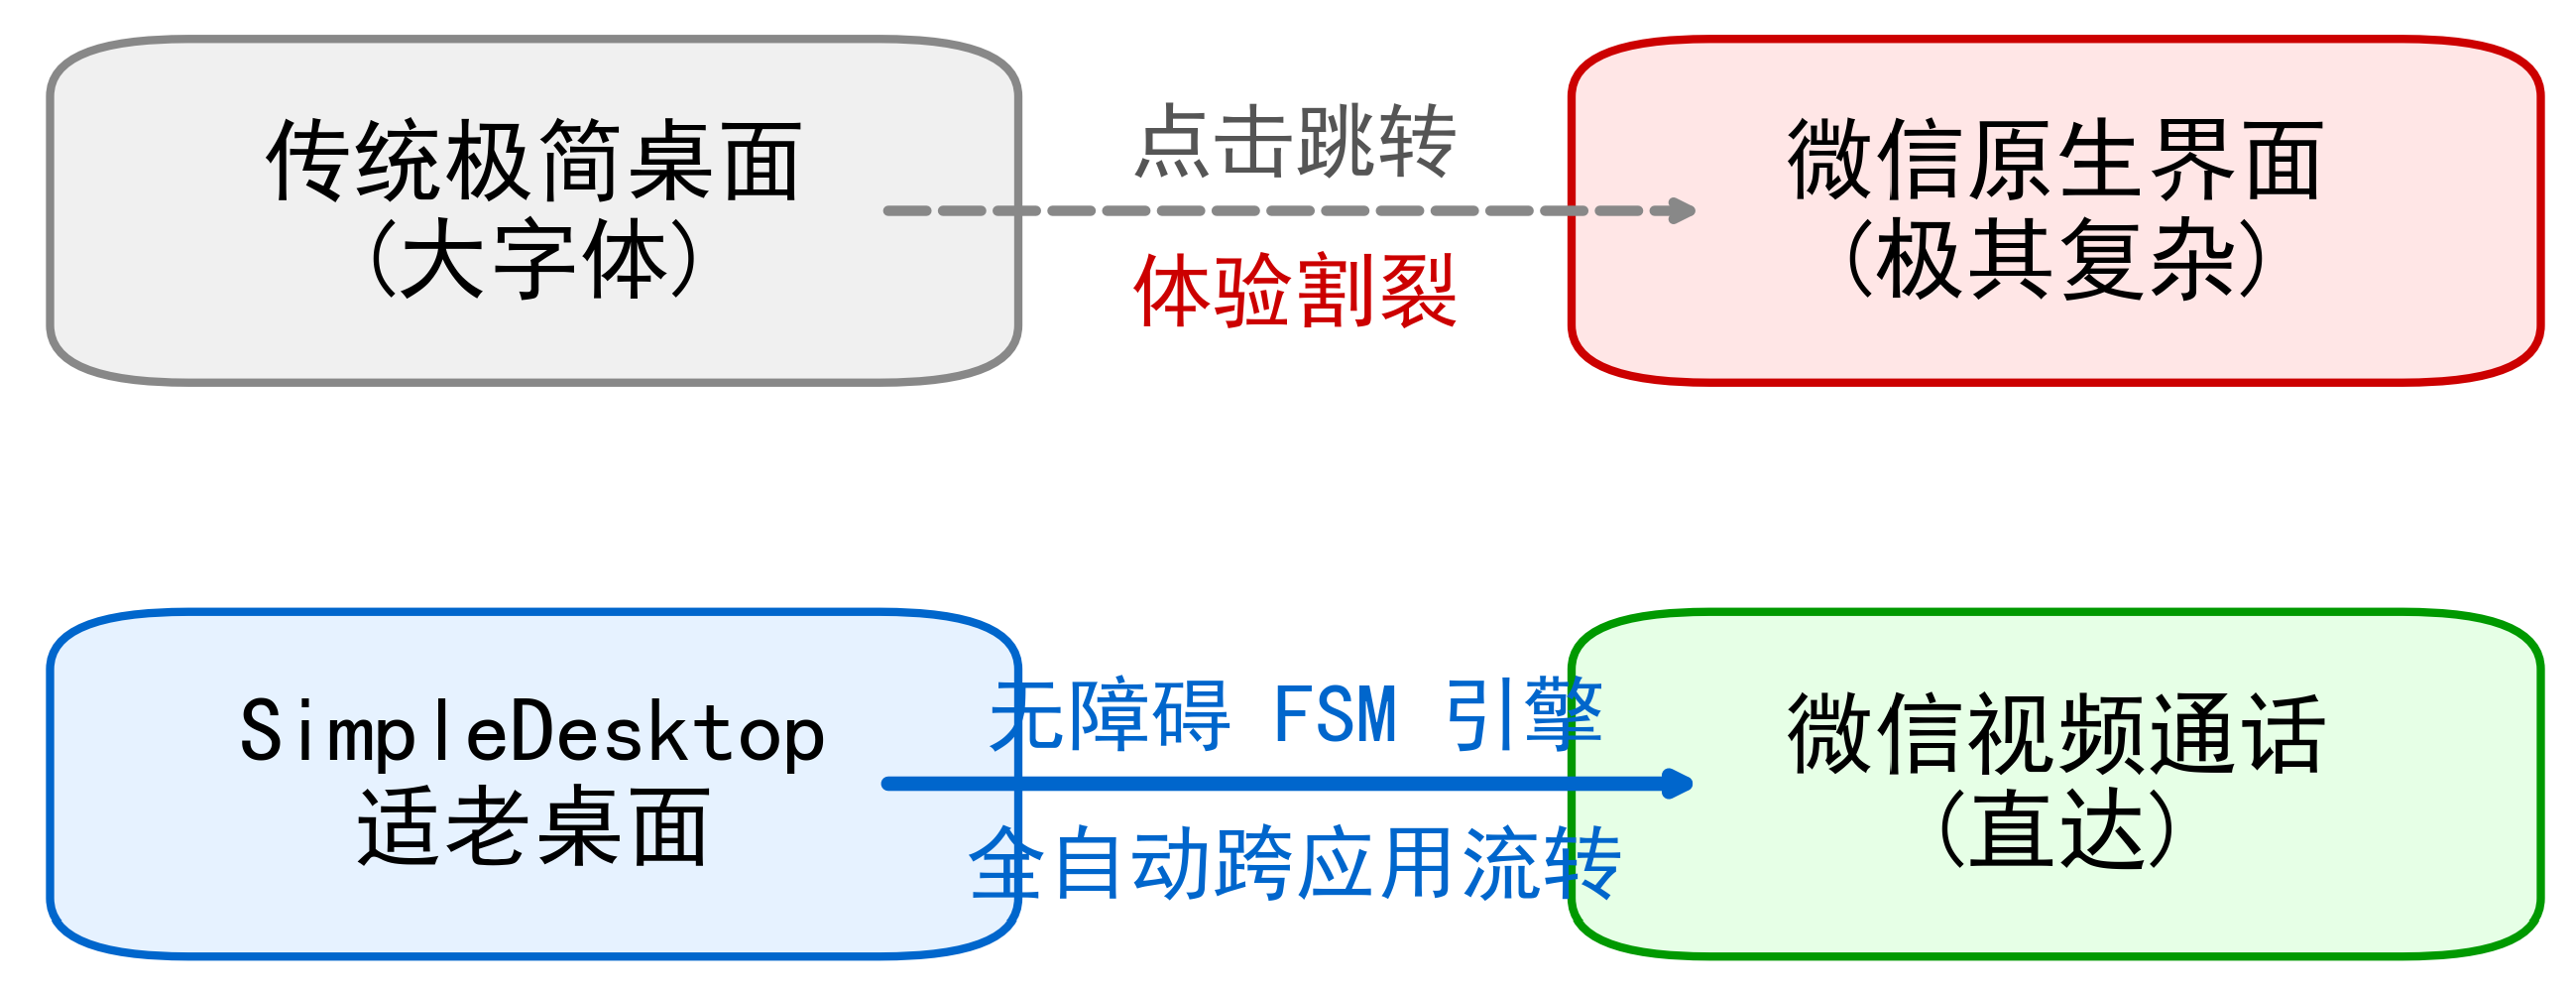
\includegraphics[width=0.9\textwidth]{figures/fig1_3_architecture_compare.png}
    \caption{传统适老化桌面与本系统自动化直达通道的体验对比}
    \label{fig:arch_compare}
\end{figure}

在学术研究层面，近年来国内外学者从多个维度围绕适老化终端展开了探索。在人因工程方向，研究者基于Fitts运动定律对老年人触控行为建立了量化模型，系统论证了增大触控目标面积与降低界面元素密度对提升操作精度的正向作用；在视觉认知方向，依据对比敏感度函数（Contrast Sensitivity Function）建立的色彩可读性评估模型，为适老配色标准的制定提供了理论依据，相关研究指出前景与背景的WCAG对比度比值维持在4.5:1以上可显著改善老年用户的文字识别率；在可用性工程方向，综合眼动追踪数据与NASA-TLX认知负荷量表的实验研究验证了界面层级简化对老年用户任务完成效率的积极影响\upcite{5,6}。

尽管如此，上述研究均聚焦于终端界面的视觉呈现与信息架构优化，较少涉及如何在保持原生应用界面不变的前提下，通过系统层的技术介入为老年用户构建更短的操作路径\upcite{8}。这一跨应用穿透与代理执行的深层次工程命题，在已有文献中尚属显著研究空白，也是本课题在现有适老化研究基础上谋求突破的核心切入点。

\subsection{Android无障碍自动化技术研究现状}
要在不修改第三方应用源码的前提下实现跨应用的操作简化，业界和学界普遍将Android平台提供的无障碍服务（AccessibilityService）视为最具可行性的技术抓手。无障碍服务是Android系统为辅助视障、肢障等特殊用户群体而设计的系统级接口，其核心能力包括：订阅并接收全局窗口内容变化、焦点切换等辅助事件，通过控件信息对象（AccessibilityNodeInfo）遍历当前界面的完整视图树（View Tree），以及向目标控件派发模拟点击、长按、文本输入、手势滑动等操作指令。由于无障碍服务随系统进程安全运行，无需root权限或USB调试连接，相较于UIAutomator等需要底层特权的自动化测试框架，其在消费级终端上的部署可行性更高，因此被广泛用于自动抢红包、自动打卡签到、辅助输入等商业场景。

然而，从已有研究与工程实践来看，当前基于无障碍服务的自动化控制方案普遍存在三方面结构性缺陷。其一是跨版本稳定性差。绝大多数实现依赖目标应用控件的静态资源标识符（Resource-ID）进行硬编码定位，一旦目标应用进行版本迭代并启用R8/ProGuard代码混淆，或底层改用Flutter、React Native等跨平台框架造成原生控件树不透明，原有定位逻辑即告失效\upcite{7}。微信作为持续高频迭代的超级应用，平均每两至三个月发布一次影响内部控件结构的大版本更新，这对硬编码方案构成了持续性的维护压力。其二是时序容错能力薄弱。现有方案多采用固定延时的线性脚本逻辑，对页面加载速度受设备性能与网络状况动态影响的客观规律缺乏适应性处理，对来电中断、系统权限弹窗、屏幕旋转等外部事件亦无动态感知与流程自恢复机制，导致在真实老年用户的复杂使用环境中流程稳定性严重不足。其三是缺乏老年场景的专项适配。已有研究与产品将无障碍服务视为开发者调试工具，而非面向终端老年用户的可靠产品能力，对老年人误触屏幕、场景切换频繁导致的焦点争抢（Focus Competition）等特殊问题缺乏针对性的防护设计，极易造成自动化流程陷入死锁。

从技术演进前沿来看，随着多模态大语言模型（Multimodal LLM）的快速发展，基于视觉-语言模型（Vision-Language Model，VLM）的图形用户界面智能体（GUI Agent）已成为无障碍自动化领域的前沿研究热点。此类方案通过对屏幕截图进行视觉理解，结合大模型的逻辑推理能力，以自然语言指令驱动跨应用自主导航，从理论上摆脱了对底层控件树结构的硬编码依赖，具备较强的跨版本泛化潜力。然而，现阶段大模型驱动的GUI自动化在端侧部署方面仍面临不可回避的工程瓶颈：典型的多模态推理模型参数量超过70亿，端侧运行显存需求通常在8GB以上，在主流适老化目标机型（中低端Android设备）上无法实现实时响应；同时，强依赖云端API调用引入了不可控的网络延迟，而老年用户的网络环境本身往往是系统需要主动守护的脆弱环节，两者形成悖论。

综合上述研究现状可以判断，尽管移动终端适老化与无障碍自动化两个方向均已取得一定进展，但"第三方应用内操作门槛高"与"现有端侧自动化方案跨版本稳定性差"之间依然横亘着显著的技术鸿沟。在通信终端无障碍交互方向，既有研究多聚焦于屏幕朗读、语音输入等单向辅助技术，对于如何利用无障碍能力主动代理老年用户完成微信通话等高频复杂操作，并保证在真实环境下的鲁棒性这一问题，缺乏系统性的工程方法论。本课题正是着眼于这一研究空白，放弃依赖Resource-ID的硬编码脆弱路径，提出并实现了以七阶段状态机建模、双通道节点检索、焦点退避与心跳防死锁为核心的多级容错自动化框架，以期在无需云端大模型支撑、无需设备特殊权限的前提下，为老年用户提供稳定、低延迟、跨版本兼容的一键直拨通信能力。



\section{主要研究内容}
针对前述移动通信终端在适老化方向上的痛点和现有研究的不足，本课题完成了一款面向老年用户的Android智能桌面系统SimpleDesktop的全栈设计与实现。系统以问题驱动为基本思路，围绕老年用户实际遇到的视觉障碍、操作障碍、通话障碍、网络障碍和交互障碍五大问题，相应展开五个方向的研究与实践。

一是面向终端架构稳定性的微内核插件化引擎研究。系统摒弃了传统单体式应用架构，将桌面信息聚合、联系人通讯、应用启动、天气服务等业务功能解耦为相互独立的功能插件，并通过统一的插件管理器和消息总线进行协调。该架构既保证了系统在低端设备上的稳定运行，也为未来扩展健康监测、智能家居控制等模块预留了清晰接口。

二是面向老年视觉与认知特征的适老化人机交互界面研究。系统基于现代声明式UI框架构建了高对比度、大字号、卡片化的桌面界面规范，支持不同字号档位与多种主题方案的实时切换，并在主屏中以聚合面板的形式集中呈现时间、农历、天气、常用联系人和常用应用，最大限度降低老年用户的视觉搜索成本。

三是面向无障碍通信的微信一键自动通话研究。针对老年用户使用微信视频通话操作步骤过多的问题，提出基于Android无障碍服务的七阶段状态机自动化方案\upcite{24,26}，配合双通道节点检索算法\upcite{30}和焦点防冲突退避机制\upcite{29}，实现桌面点击联系人、系统自动完成全部微信操作、直接进入视频通话的一键化流程。

四是面向终端通信连续性的WiFi网络守护研究。系统通过常驻前台服务持续监测网络连接状态，一旦检测到WiFi断连便进入宽限期等待自动恢复；超过宽限期后，借助无障碍服务自动开启WiFi开关，并通过弹窗与语音播报双重通道引导用户进行必要的人工干预，从而最大限度保障通信链路的连续性。

五是面向自然语言交互的语音助手研究。系统基于Android原生TTS引擎实现全局语音播报，并通过关键词匹配与编辑距离容错相结合的轻量级语义解析方法\upcite{13}，将打电话给某某等自然语言指令准确映射到具体的通信操作上，使老年用户无需依赖屏幕触控即可完成主要操作。

\begin{figure}[htbp]
    \centering
    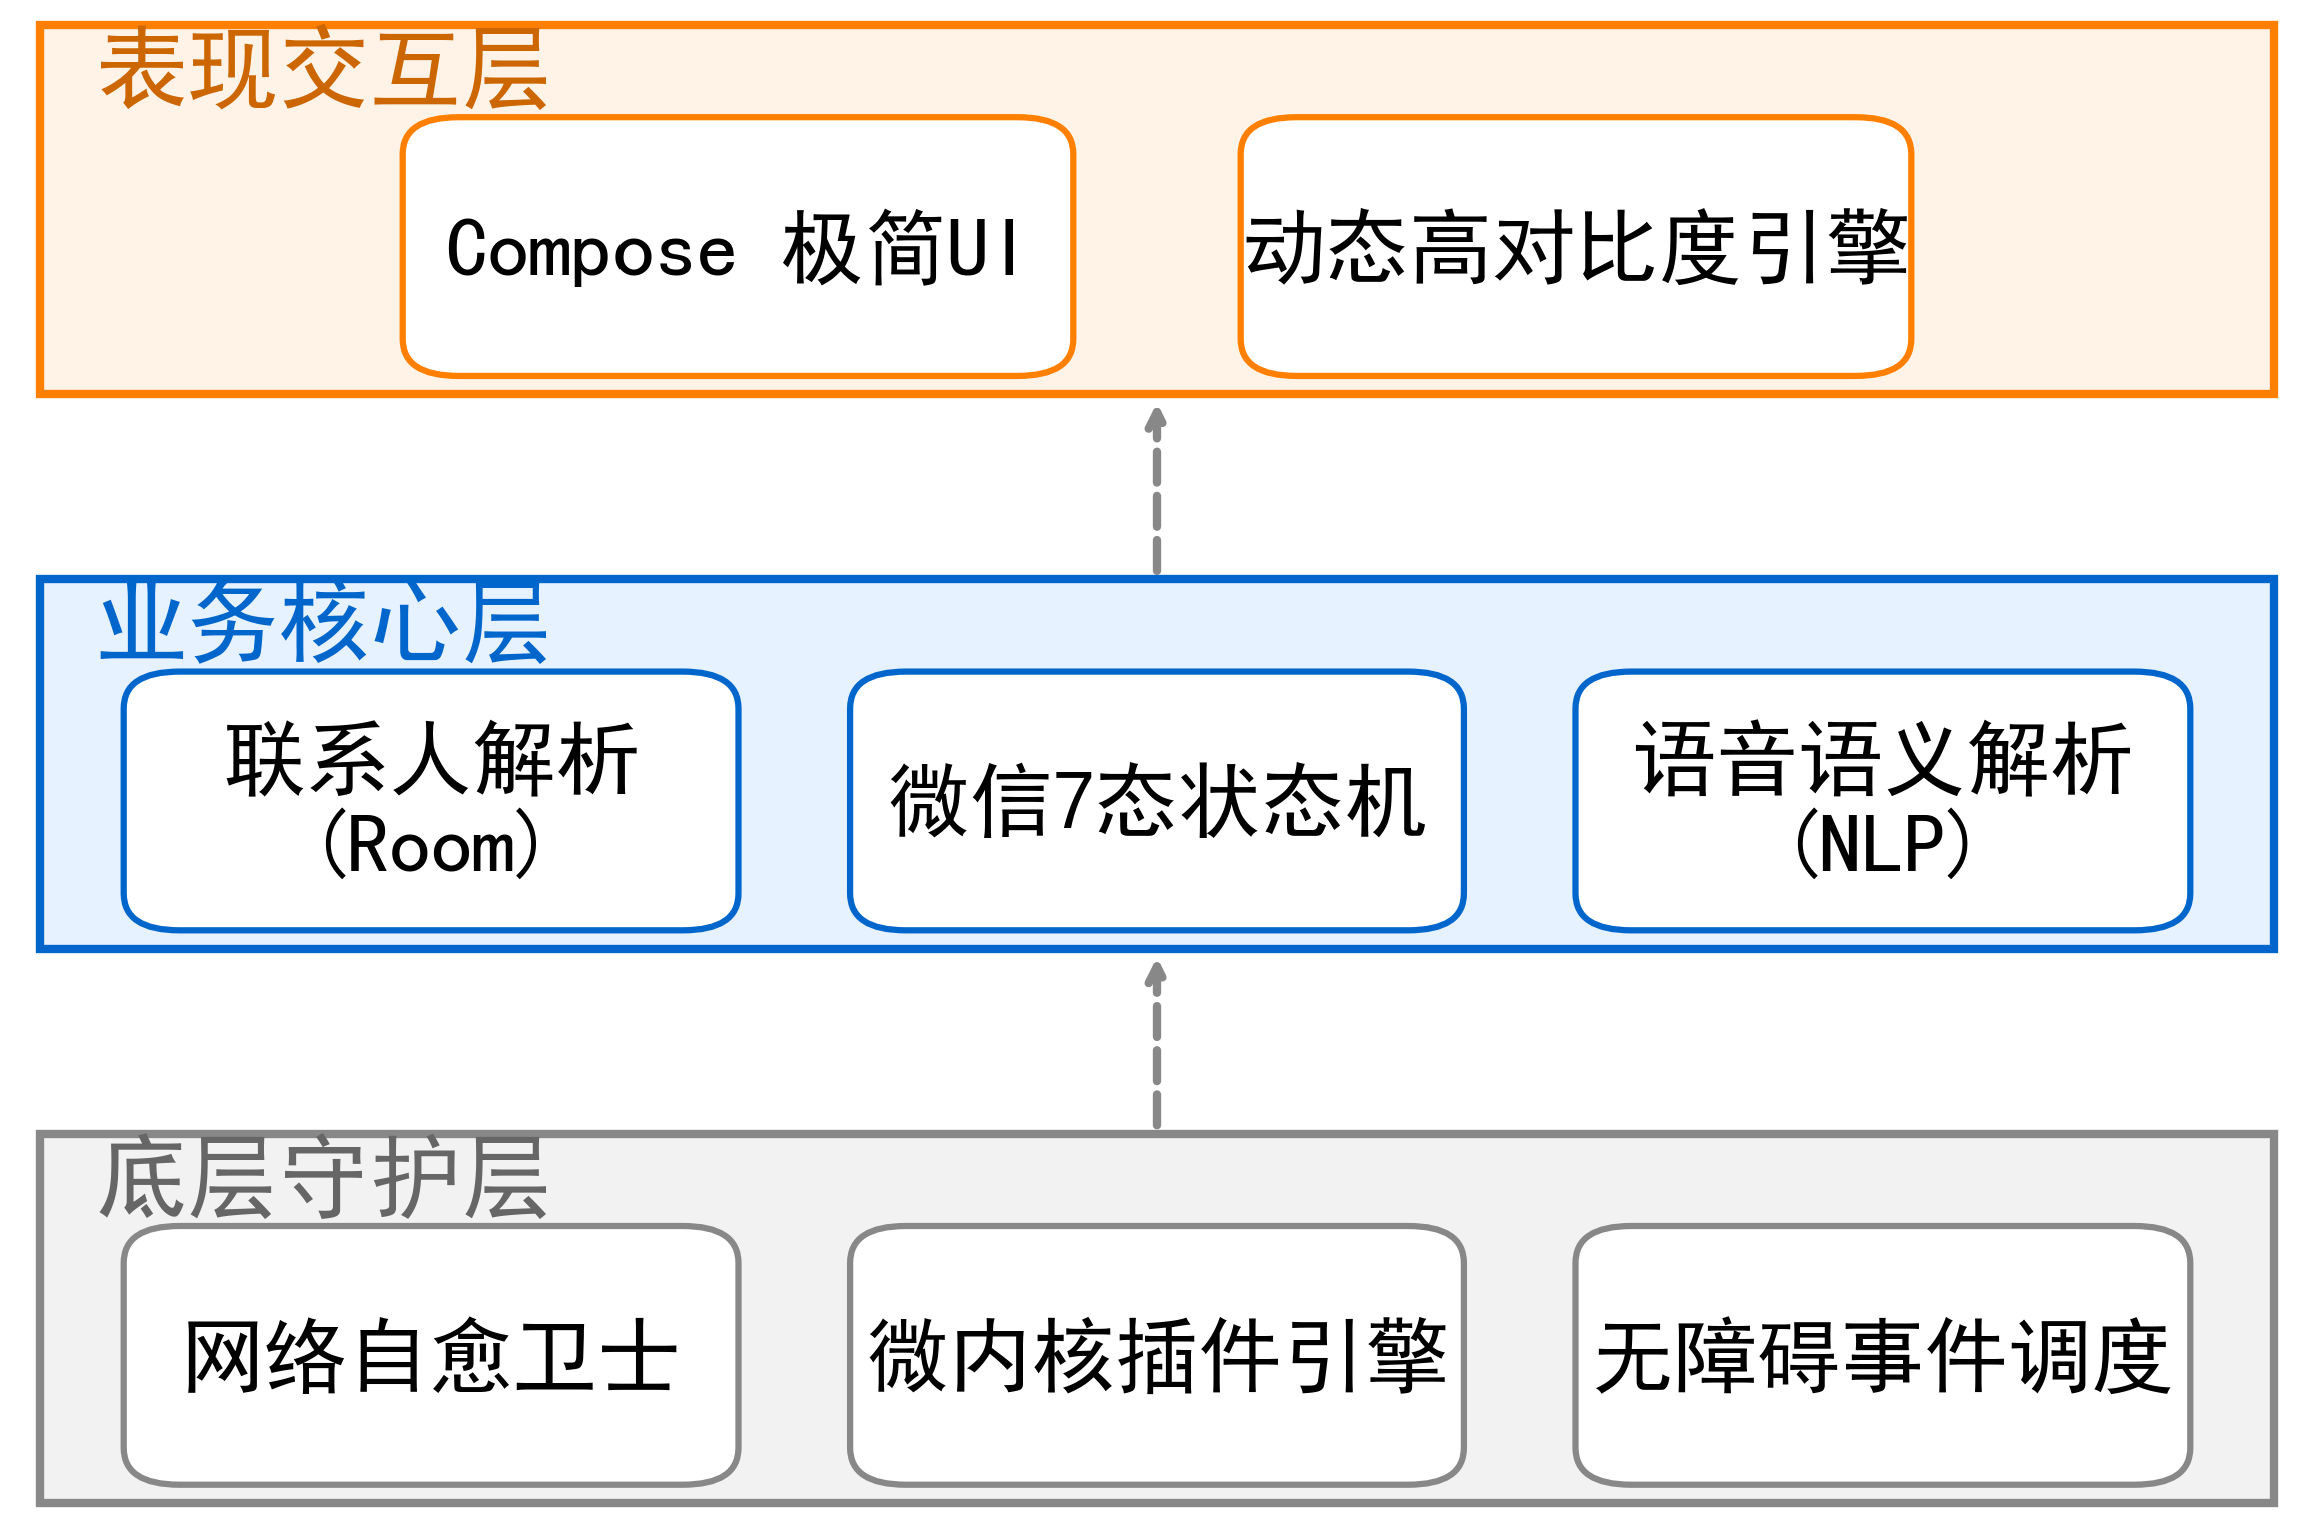
\includegraphics[width=0.9\textwidth]{figures/fig1_4_system_overview.png}
    \caption{SimpleDesktop 系统技术全景架构图}
    \label{fig:system_overview}
\end{figure}

\section{论文组织结构}
全文共分五章，各章主要内容如下。

第1章为绪论，主要介绍课题的研究背景、研究意义、国内外研究现状、主要研究内容以及论文的组织结构，旨在明确研究的出发点与全文的整体脉络。

第2章为技术基础，主要介绍本课题所依赖的技术体系，包括现代Android技术栈、数据持久化与依赖注入框架、微内核插件化架构理论以及Android无障碍服务的基本原理，为后续章节的设计与实现奠定理论与技术基础。

第3章为适老化智能桌面系统的设计与实现，是论文的核心章节。首先从老年用户视角出发开展需求分析，然后给出宿主层、总线层、插件层三层架构的整体设计方案并交代开发环境，接着分别对适老化界面、微信自动化直连、WiFi网络守护、语音辅助等核心功能模块进行设计与实现的详细阐述，最后给出软件的整体操作流程。

第4章为软件测试与分析，依次从功能测试、兼容性测试和性能测试三个维度对系统质量进行系统化评估。功能测试覆盖联系人增删改查、应用管理、微信通话发起、语音指令解析等核心用例；兼容性测试覆盖不同型号、不同分辨率、不同系统版本的真机环境；性能测试关注响应时间、页面加载速度以及多并发访问的处理能力。

第5章为总结与展望。首先对全文工作进行总结，凝练课题的主要成果与贡献；其次客观分析当前系统存在的局限性，并对未来的研究方向作出展望。









































\iffalse

\chapter{绪论}
\section{研究背景与意义}
\subsection{人口老龄化加剧下的移动通信终端使用困境}
伴随我国人口结构的深刻变化，老龄化已成为关乎国计民生的重要社会议题。根据国家统计局发布的数据，截至2023年末，我国60岁及以上人口已达2.97亿，占总人口的21.1\,\%\upcite{1}，预计到2035年这一比例将突破30\%，我国正稳步迈向中度老龄化社会。在通信技术高速发展的背景下，移动通信终端早已超越传统的语音通话功能，演变为集即时通讯、移动支付、远程医疗、出行导航等多重服务于一体的综合数字生活入口，深度融入了现代社会的各个角落。


\begin{figure}[htbp]
    \centering
    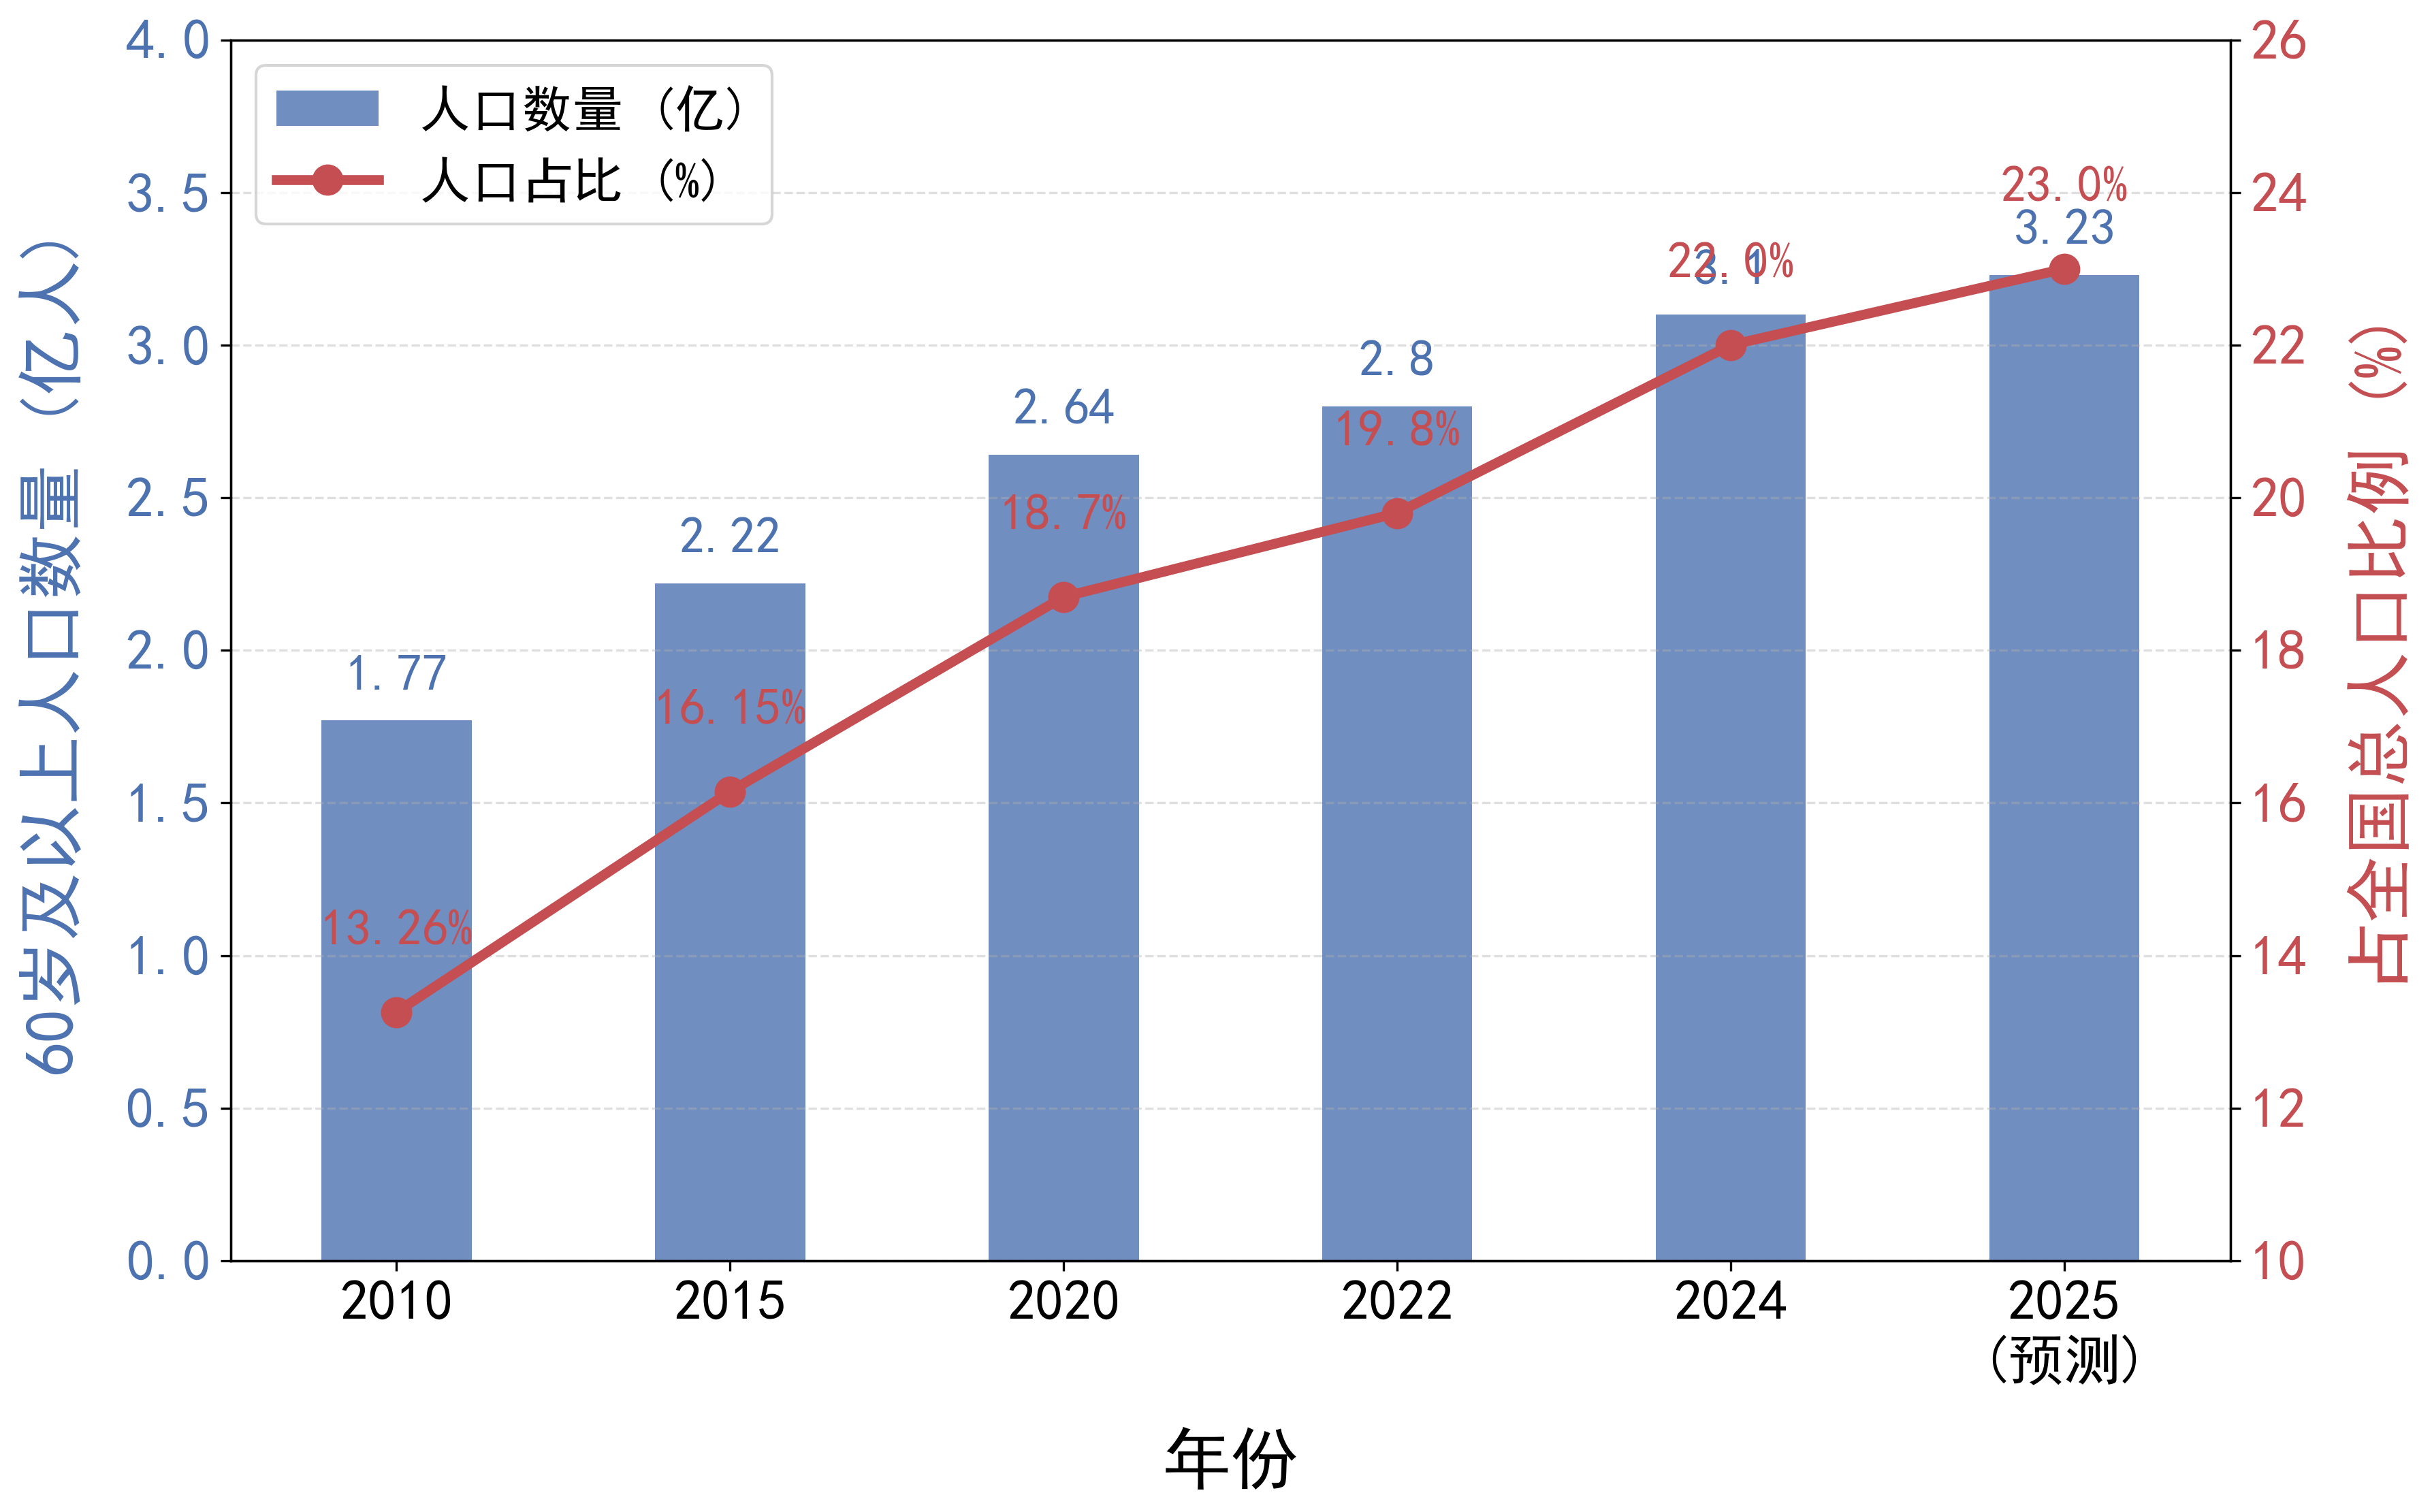
\includegraphics[width=0.85\textwidth]{figures/fig1_1_aging_population_trend.png}
    \caption{中国60岁及以上老年人口数量与占比趋势 (2010-2025)}
    \label{fig:aging_population}
\end{figure}


然而，移动终端功能的不断丰富在为大多数用户带来便利的同时，也对老年群体形成了日益突出的使用障碍。一方面，老年用户由于生理机能退化，普遍面临视力下降、听力减弱、手指灵活性降低、认知反应速度减缓等客观问题；另一方面，主流智能终端的人机交互界面设计往往以年轻用户为主要目标群体，密集的图标布局、多层嵌套的菜单结构、频繁的系统弹窗以及不断变化的应用更新，对老年人构成了显著的认知负担与操作障碍。

这种由技术快速演进与老年群体适应能力之间的差异所形成的隔阂，被学界称为“数字鸿沟”。数字鸿沟在通信领域的具体体现，包括老年人无法独立完成视频通话、容易误触系统设置导致网络中断、难以理解陌生应用界面、对授权弹窗与广告推送缺乏判断能力等。中国互联网络信息中心发布的第52次中国互联网络发展状况统计报告指出，60岁及以上网民群体占比仅为14.3\,\%\upcite{2}，远低于其在总人口中的比例，说明大量老年人在数字化浪潮中处于事实上的边缘化状态。

在通信工程专业视角下，移动通信终端不仅是数据交换的物理载体，更是承载用户与外界保持联络、获取信息、维系情感的关键媒介。如何通过终端层面的软件再设计，让老年用户重新获得对智能设备的掌控感与安全感，使其能够便捷地完成与子女的视频通话、稳定地接入家庭无线网络、流畅地使用日常应用，是当代通信工程从业者必须正视的现实命题。

\subsection{适老化痛点剖析}
从一线调研结果看，老年用户在使用主流智能手机过程中暴露出的核心痛点可归纳为以下几个方面。其一是视觉痛点，标准界面字号偏小、图标密集，导致老年人需要佩戴眼镜并凑近屏幕才能勉强辨识，长时间使用容易引发视疲劳。其二是认知痛点，多级菜单和大量弹窗使老年人难以判断当前所处的界面位置，操作过程极易迷失方向。其三是通话痛点，微信视频通话需要至少七步操作，老年人记不住流程，需要子女多次教学方能勉强掌握。其四是网络痛点，老年人误触WiFi开关后无法自行恢复连接，长时间断网而不自知，错过重要来电。其五是交互痛点，对触摸屏操作不熟练，时常出现误触或长按引发的意外操作，进一步加剧对智能设备的不安全感。

\begin{figure}[htbp]
    \centering
    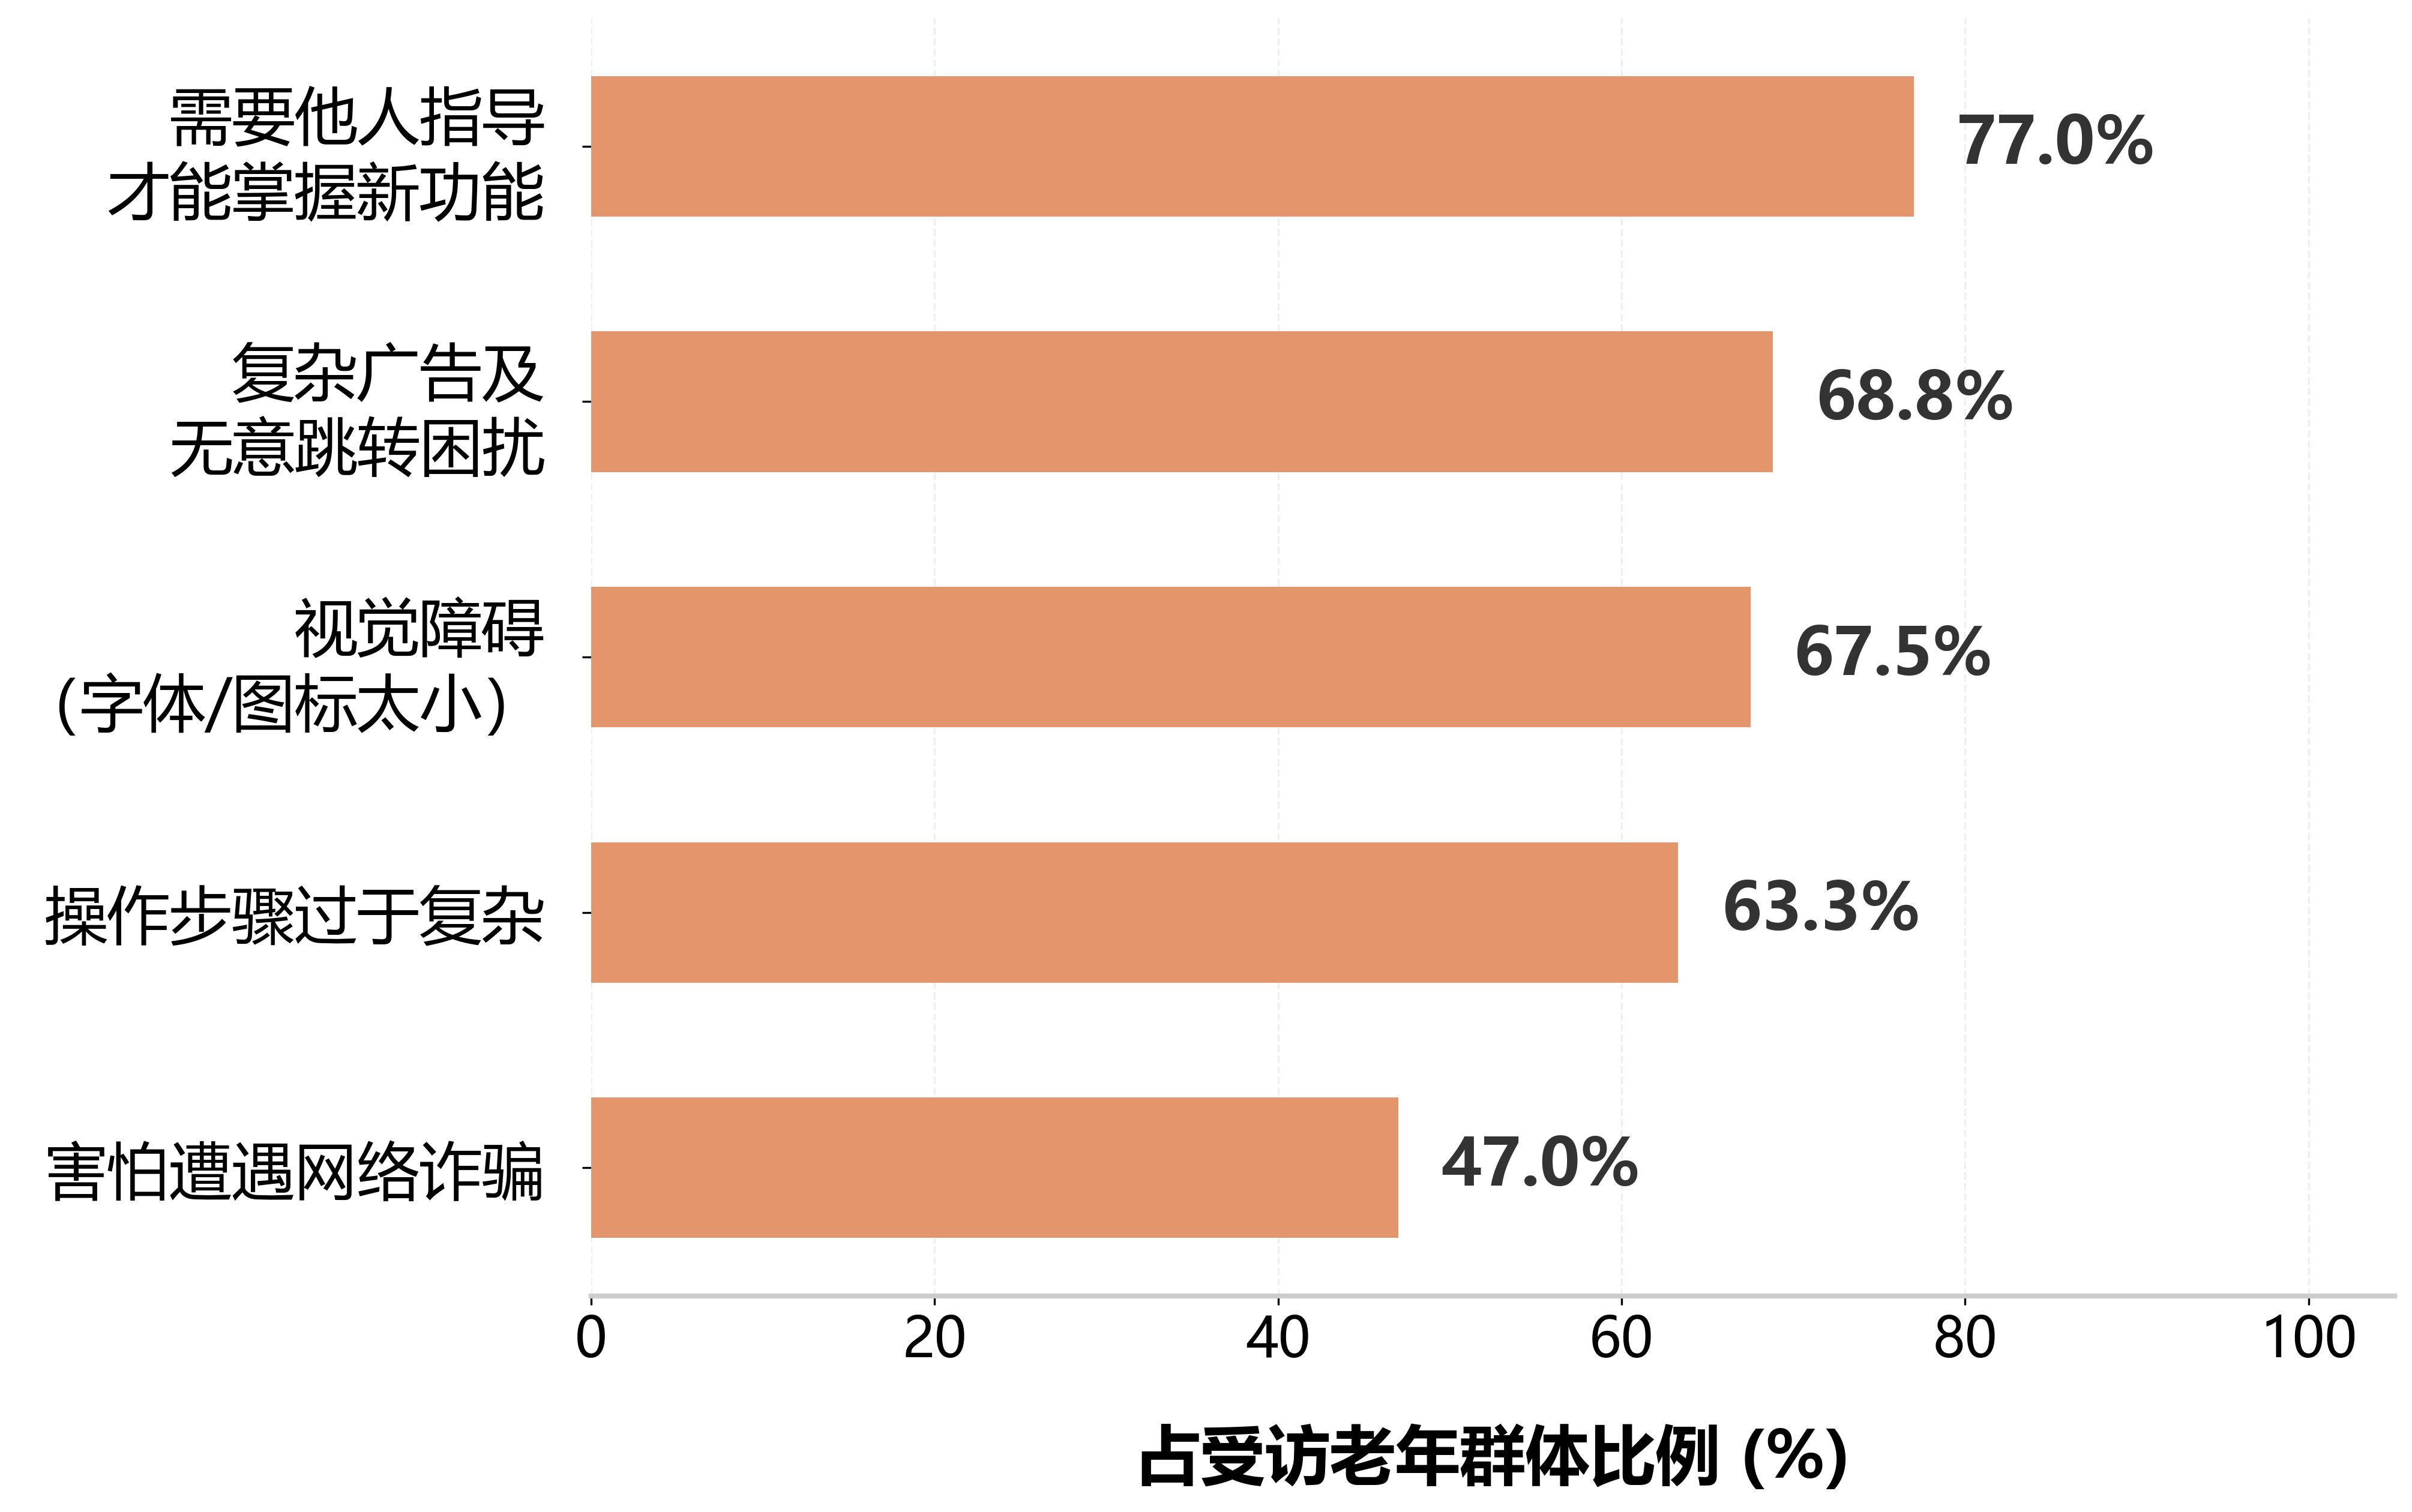
\includegraphics[width=0.85\textwidth]{figures/fig1_2_usage_pain_points.png}
    \caption{老年人智能手机使用核心痛点分布}
    \label{fig:pain_points}
\end{figure}

这些痛点的共同本质在于：现有移动通信终端的软件设计未能充分考虑老年用户的认知特征与使用习惯。仅仅通过放大字号、增大图标的浅层适老化改造，无法从根本上解决问题。必须从系统架构、交互逻辑、自动化能力等多个层面进行深度重构，才能真正为老年用户提供一款能用、好用、爱用的移动通信终端。这正是本课题立项的现实出发点。

\subsection{研究意义}
本课题以适老化智能桌面系统的设计与实现为研究对象，其意义可从社会价值、工程价值与学术价值三个维度展开。从社会价值层面看，本研究致力于通过软件技术手段帮助老年群体跨越数字鸿沟，让通信技术真正服务于全民福祉。当系统能够将原本繁琐的微信视频通话操作简化为一次点击、能够在网络异常时主动恢复并向用户清晰提示，老年用户便能更安心地依赖移动终端与家人保持联系，独居老人的精神慰藉与紧急求助通道也得到了实质性保障，这对于构建友好型老龄化社会具有积极意义。

从工程价值层面看，本课题摒弃了传统适老化方案“放大字号、堆叠图标”的简单做法，转而从系统架构与人机交互两个维度同步发力。通过自研的微内核插件化架构，系统在功能扩展性与运行稳定性方面取得了良好平衡，能够适配从千元入门机到主流旗舰机型的多种硬件配置；通过Android无障碍服务深度整合的微信一键直拨方案，系统从交互层面真正消除了老年用户的认知负担，为同类终端应用的设计提供了可复用的工程范式。

从学术价值层面看，本研究在通信终端无障碍交互、跨应用自动化控制、网络稳定性自愈等方向进行了有益探索。所提出的七阶段状态机驱动的自动化控制模型、双通道节点检索方法以及分层防御的网络守护机制，丰富了适老化通信终端研究的理论与实践成果，对推动我国老年友好型移动通信生态建设具有借鉴意义。

\section{国内外研究现状}
\subsection{移动通信终端适老化研究现状}
终端适老化是一个跨越通信工程、人机交互、工业设计等多学科的研究方向。从国际范围来看，欧美国家由于步入老龄化社会较早，相关研究起步亦较早。日本与德国的研究机构较早提出了“通用设计”理念，主张通过通用化的界面与功能设计兼顾各年龄段用户的使用需求。在产品形态上，海外市场出现了Doro、Jitterbug等专注于老年用户的终端品牌，以及Big Launcher、Simple Launcher等第三方桌面应用，其设计思路普遍以大尺寸瓷砖式布局取代传统的网格图标布局，并精简非必要功能入口。然而，海外方案在中国本土的适用性较为有限，例如其无法对国内老年用户高度依赖的微信、支付宝等应用进行深度适配，也难以兼容中国传统农历、节气等本土文化要素。

国内方面，伴随老龄化进程的加快和工信部“互联网应用适老化改造”专项行动\upcite{3}的推进，主流手机厂商相继推出了系统级适老化方案。华为的“简易模式”、小米的“极简模式”、OPPO的“简单模式”以及荣耀的“长辈模式”等，均对系统字号、图标尺寸、铃音音量等进行了适当优化，并在拦截骚扰电话、识别诈骗短信等方面提供了一定支持。但这些厂商方案的共同局限在于，其作用范围仅限于操作系统层面，无法穿透至第三方应用内部。换言之，老年用户进入微信、支付宝等具体应用后，依然需要面对其原本的复杂界面，操作障碍并未得到根本解决。

\begin{figure}[htbp]
    \centering
    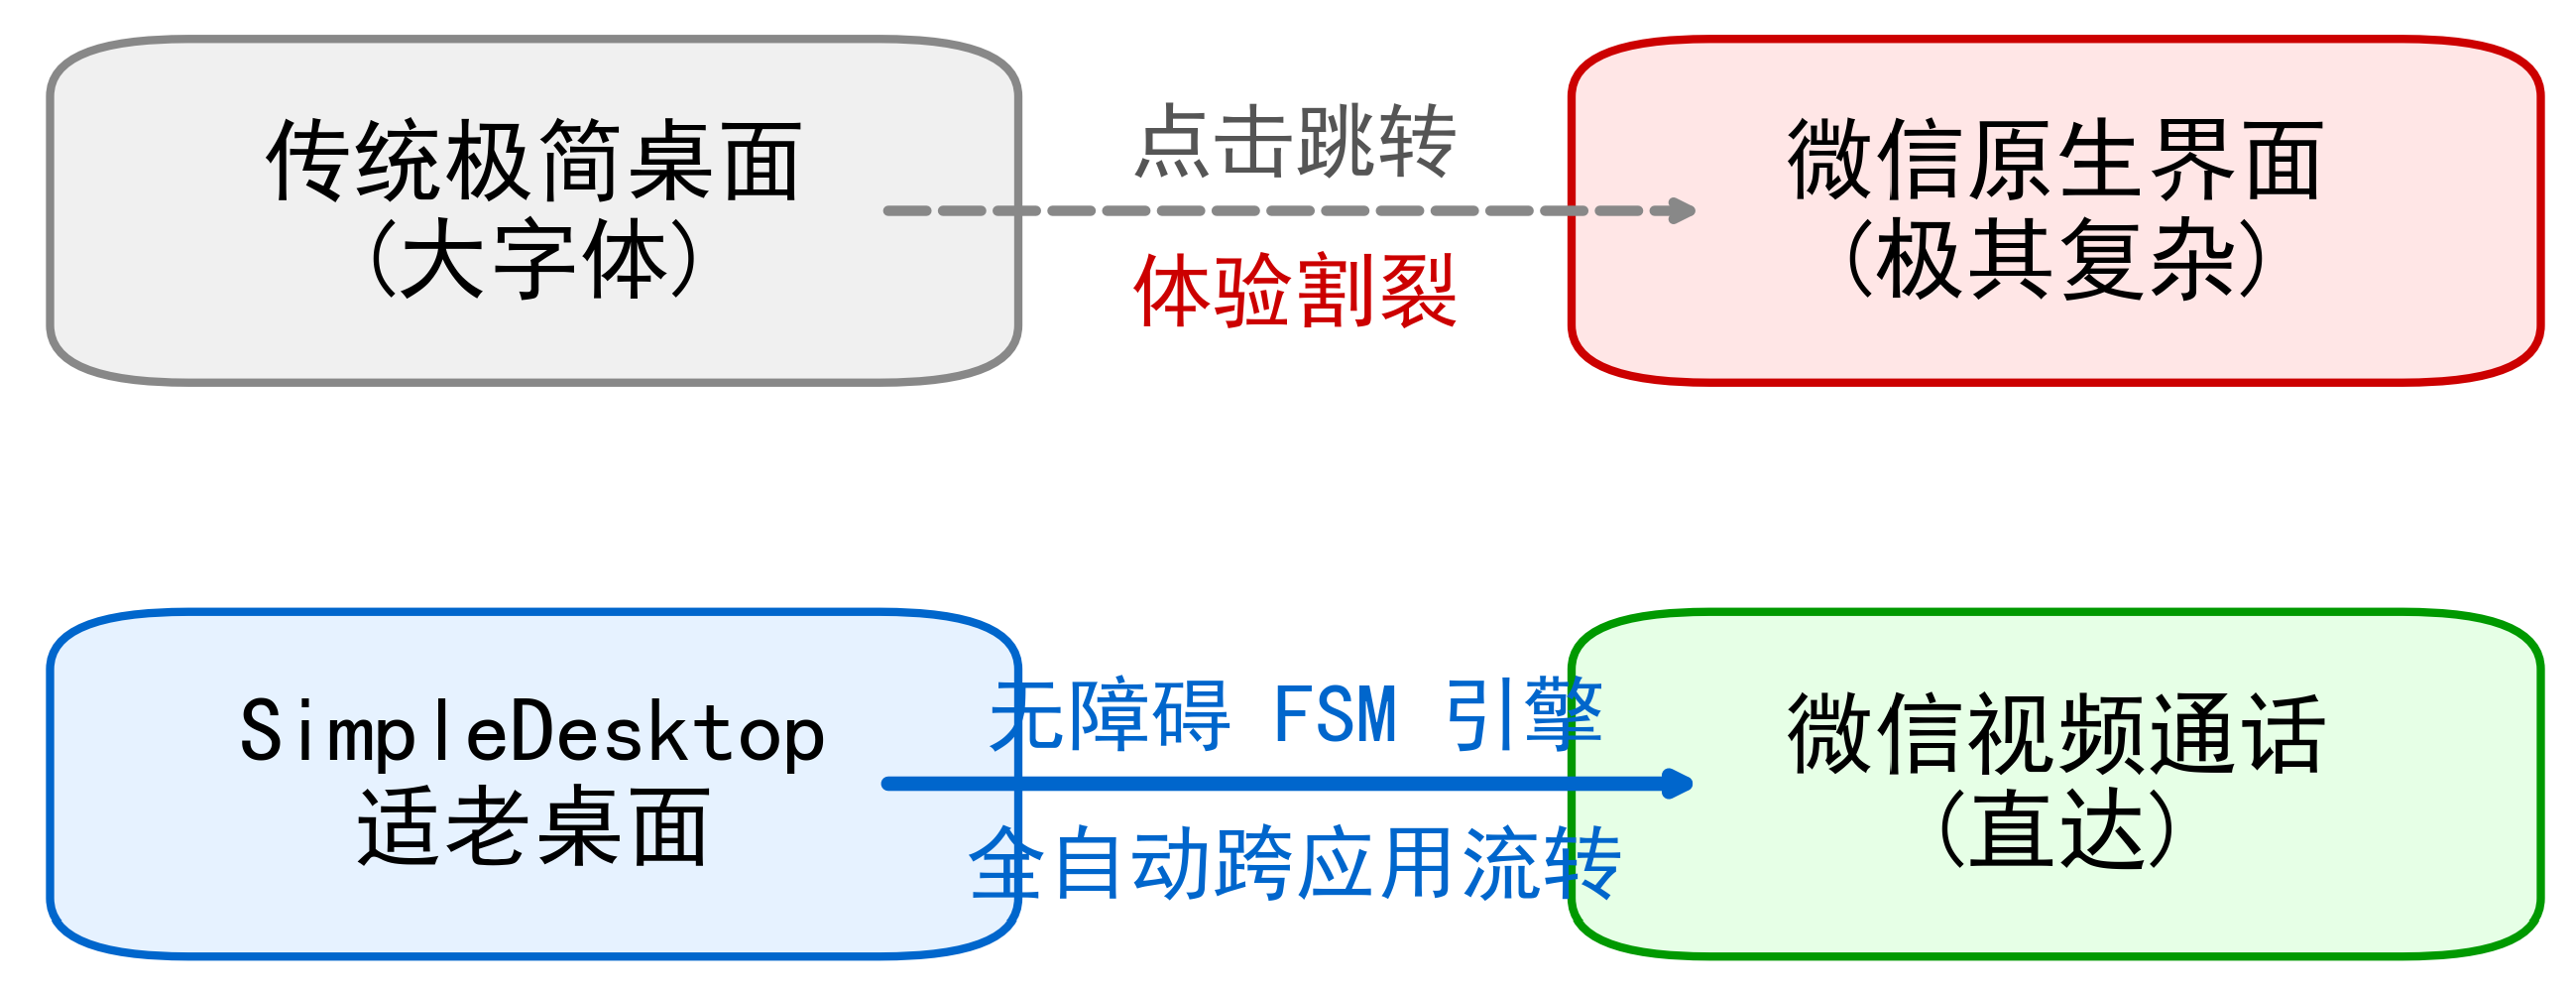
\includegraphics[width=0.9\textwidth]{figures/fig1_3_architecture_compare.png}
    \caption{传统适老化桌面与本系统自动化直达通道的体验对比}
    \label{fig:arch_compare}
\end{figure}

在学术研究方面，近年来国内外学者围绕适老化终端开展了多方面探索。文献研究普遍聚焦于以下三个方向：一是基于Fitts定律的触控目标尺寸优化，从生理人因学角度论证大按钮设计的合理性；二是基于对比敏感度模型的色彩搭配研究，提出适合老年视觉特征的高对比度配色方案；三是基于眼动追踪与可用性测试的界面布局评估，验证简化界面对老年用户操作效率的提升效果。然而，相关研究多聚焦于界面表层的视觉优化\upcite{4,5,6}，鲜有研究涉及如何让老年人在第三方应用内部也能享受到简化体验这一深层次命题\upcite{8}。

\subsection{Android无障碍自动化技术研究现状}
要实现跨第三方应用的操作简化，业界普遍采用Android平台提供的无障碍服务作为技术抓手。无障碍服务最初是为视障用户提供屏幕朗读功能而设计的系统级接口，但因其具备读取屏幕控件树和执行模拟操作的能力，近年来被广泛应用于自动抢红包、自动签到、自动化测试等多种场景。

从已有的研究与产品实践来看，基于无障碍服务的自动化控制方案主要存在以下不足：首先，绝大多数实现方式依赖目标应用控件的资源标识符进行硬编码定位，一旦目标应用版本更新或启用代码混淆，自动化流程便会迅速失效；其次，缺乏对系统级弹窗、来电中断等异常情况的容错处理机制，导致流程稳定性较差；再次，普遍缺乏对老年用户场景的针对性优化，未能将自动化能力转化为面向终端用户的简洁可靠服务。

在通信终端无障碍交互方向上，既有研究多关注屏幕朗读、语音输入等输入输出层面的辅助技术，对于如何利用无障碍能力构建稳定可靠的跨应用通信桥接这一问题，缺乏系统性的工程方案。本课题正是着眼于这一研究空白，探索通过状态机建模、双通道检索、焦点退避等机制，构建具备较高鲁棒性的适老化终端自动化通信能力。

\section{主要研究内容}
针对前述移动通信终端在适老化方向上的痛点和现有研究的不足，本课题完成了一款面向老年用户的Android智能桌面系统SimpleDesktop的全栈设计与实现。系统以问题驱动为基本思路，围绕老年用户实际遇到的视觉障碍、操作障碍、通话障碍、网络障碍和交互障碍五大问题，相应展开五个方向的研究与实践。

一是面向终端架构稳定性的微内核插件化引擎研究。系统摒弃了传统单体式应用架构，将桌面信息聚合、联系人通讯、应用启动、天气服务等业务功能解耦为相互独立的功能插件，并通过统一的插件管理器和消息总线进行协调。该架构既保证了系统在低端设备上的稳定运行，也为未来扩展健康监测、智能家居控制等模块预留了清晰接口。

二是面向老年视觉与认知特征的适老化人机交互界面研究。系统基于现代声明式UI框架构建了高对比度、大字号、卡片化的桌面界面规范，支持不同字号档位与多种主题方案的实时切换，并在主屏中以聚合面板的形式集中呈现时间、农历、天气、常用联系人和常用应用，最大限度降低老年用户的视觉搜索成本。

三是面向无障碍通信的微信一键自动通话研究。针对老年用户使用微信视频通话操作步骤过多的问题，提出基于Android无障碍服务的七阶段状态机自动化方案，配合双通道节点检索算法和焦点防冲突退避机制，实现桌面点击联系人、系统自动完成全部微信操作、直接进入视频通话的一键化流程。

四是面向终端通信连续性的WiFi网络守护研究。系统通过常驻前台服务持续监测网络连接状态，一旦检测到WiFi断连便进入宽限期等待自动恢复；超过宽限期后，借助无障碍服务自动开启WiFi开关，并通过弹窗与语音播报双重通道引导用户进行必要的人工干预，从而最大限度保障通信链路的连续性。

五是面向自然语言交互的语音助手研究。系统基于Android原生TTS引擎实现全局语音播报，并通过关键词匹配与编辑距离容错相结合的轻量级语义解析方法，将打电话给某某等自然语言指令准确映射到具体的通信操作上，使老年用户无需依赖屏幕触控即可完成主要操作。

\begin{figure}[htbp]
    \centering
    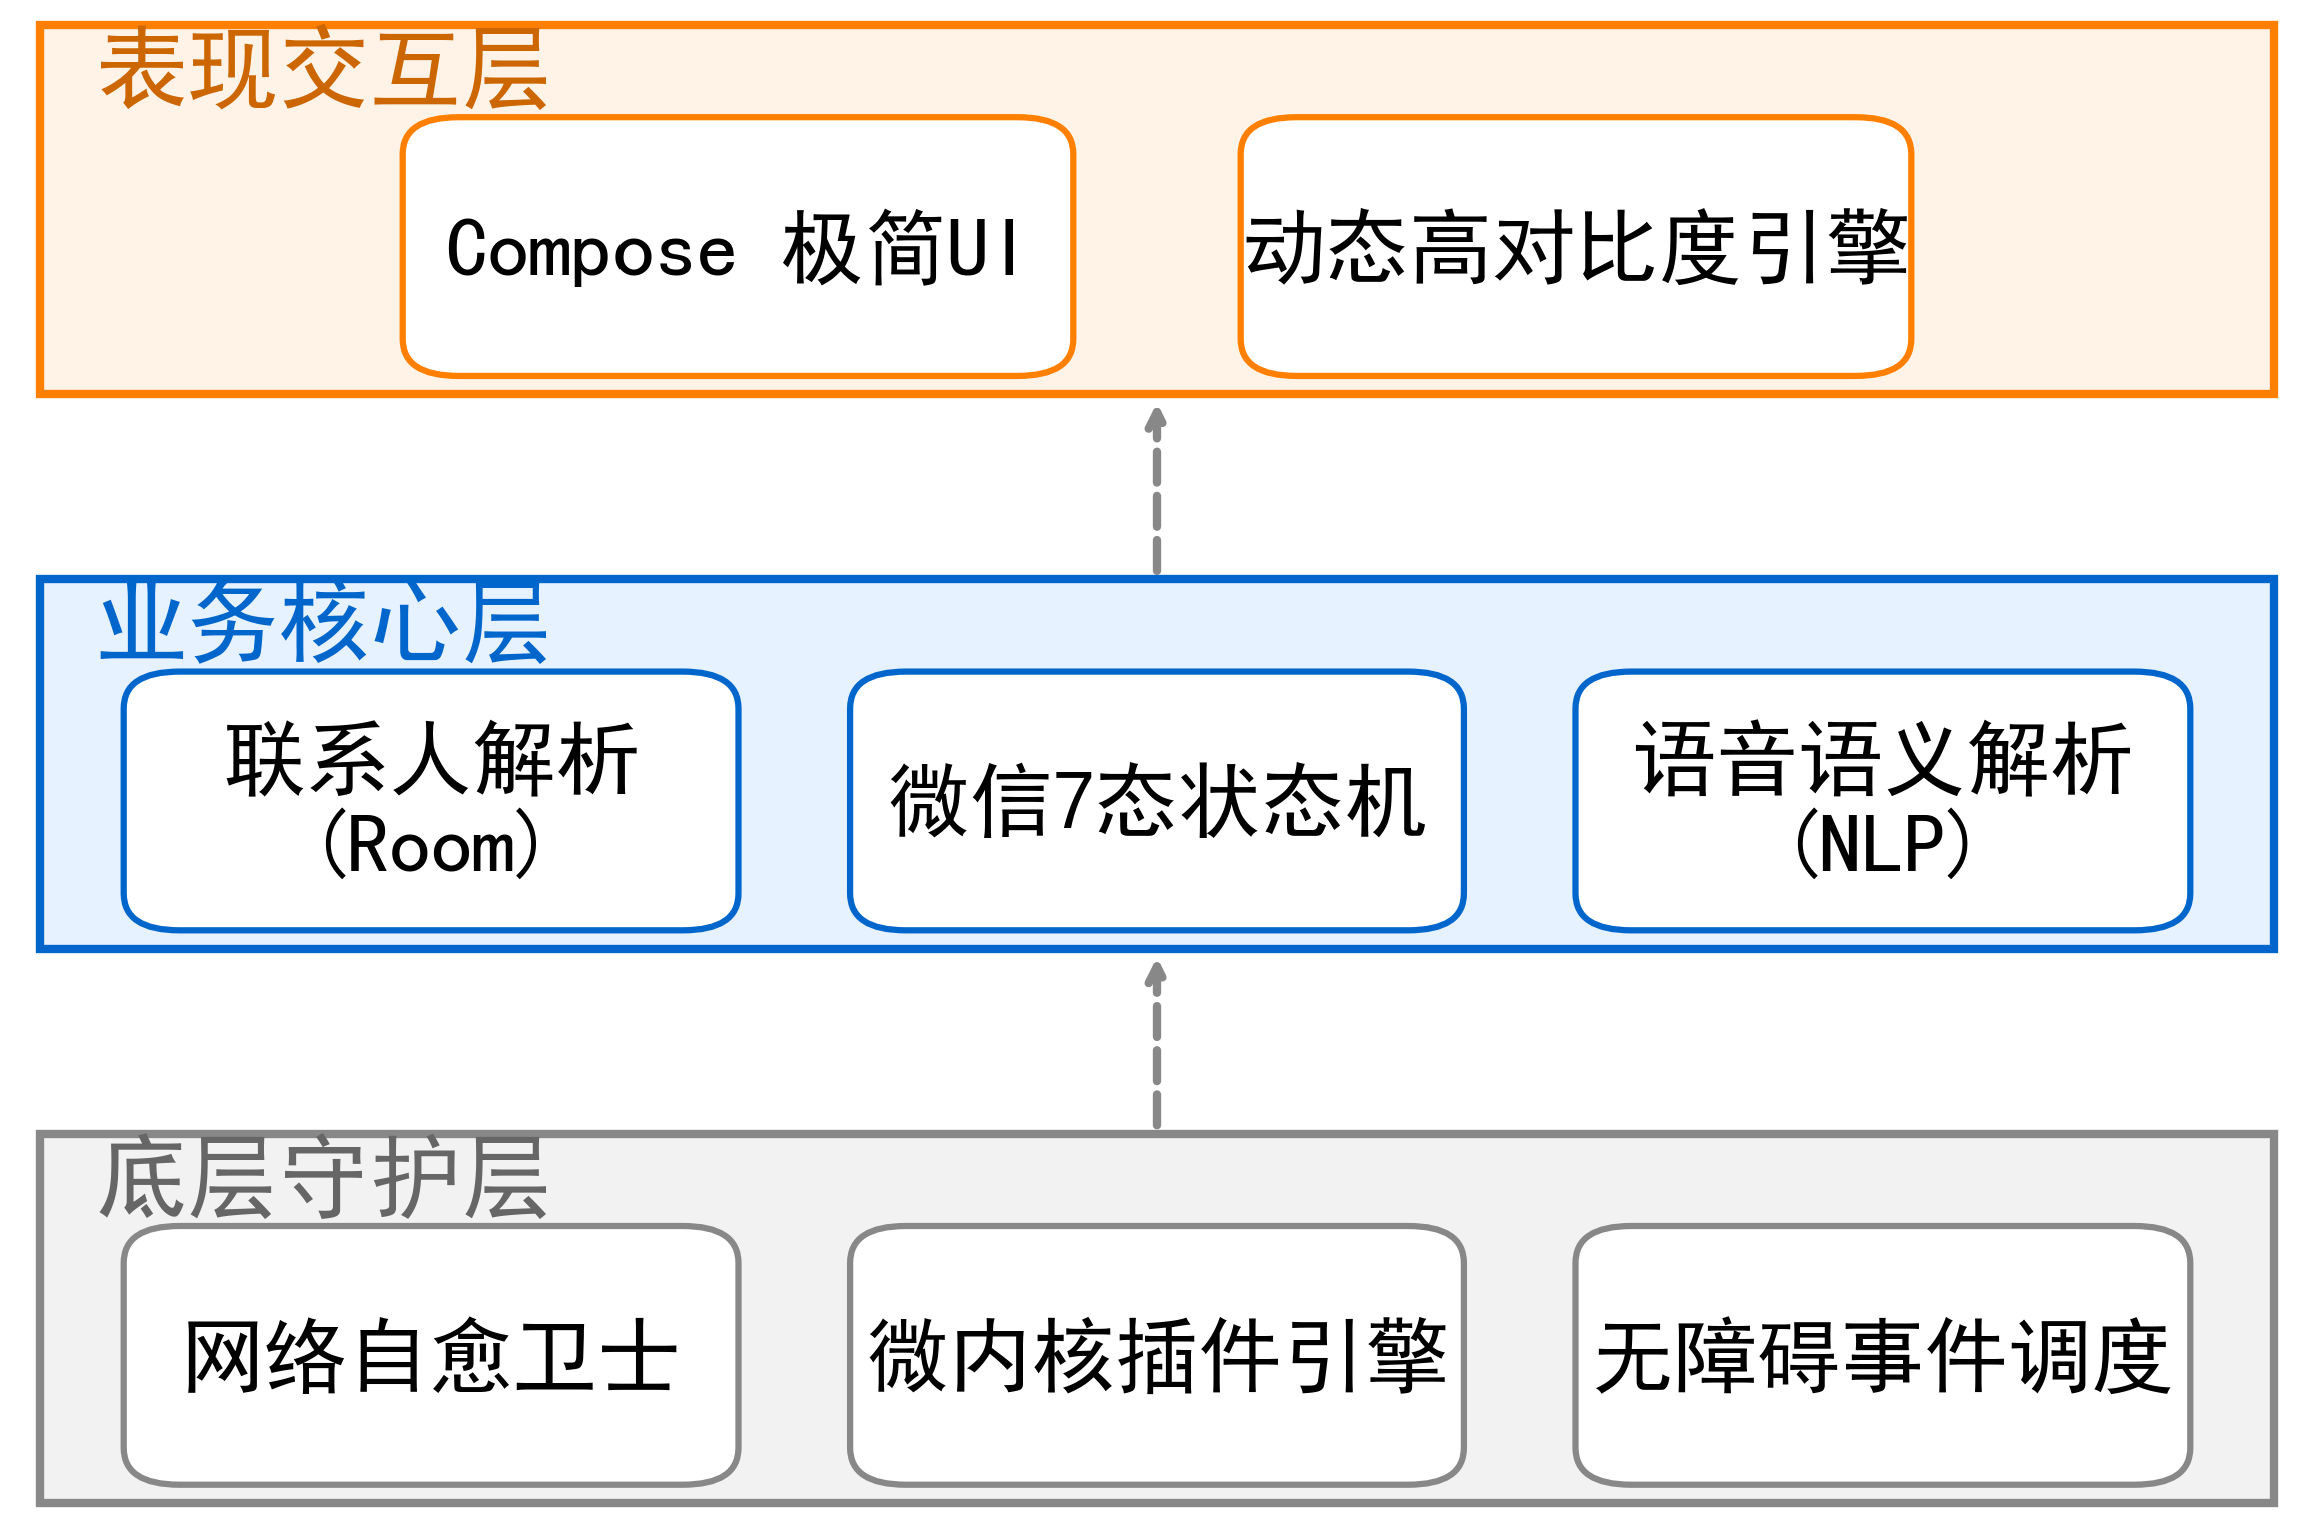
\includegraphics[width=0.9\textwidth]{figures/fig1_4_system_overview.png}
    \caption{SimpleDesktop 系统技术全景架构图}
    \label{fig:system_overview}
\end{figure}

\section{论文组织结构}
全文共分五章，各章主要内容如下。

第1章为绪论，主要介绍课题的研究背景、研究意义、国内外研究现状、主要研究内容以及论文的组织结构，旨在明确研究的出发点与全文的整体脉络。

第2章为技术基础，主要介绍本课题所依赖的技术体系，包括现代Android技术栈、数据持久化与依赖注入框架、微内核插件化架构理论以及Android无障碍服务的基本原理，为后续章节的设计与实现奠定理论与技术基础。

第3章为适老化智能桌面系统的设计与实现，是论文的核心章节。首先从老年用户视角出发开展需求分析，然后给出宿主层、总线层、插件层三层架构的整体设计方案并交代开发环境，接着分别对适老化界面、微信自动化直连、WiFi网络守护、语音辅助等核心功能模块进行设计与实现的详细阐述，最后给出软件的整体操作流程。

第4章为软件测试与分析，依次从功能测试、兼容性测试和性能测试三个维度对系统质量进行系统化评估。功能测试覆盖联系人增删改查、应用管理、微信通话发起、语音指令解析等核心用例；兼容性测试覆盖不同型号、不同分辨率、不同系统版本的真机环境；性能测试关注响应时间、页面加载速度以及多并发访问的处理能力。

第5章为总结与展望。首先对全文工作进行总结，凝练课题的主要成果与贡献；其次客观分析当前系统存在的局限性，并对未来的研究方向作出展望。


\begin{table}
    \small
    \caption{表格内换行文字单倍行距测试}
    \label{tab:linebreak_test}
    \begin{threeparttable}
    \begin{tabular}{c p{4cm} p{4cm}}
        \toprule
        \tableheader{编号} & \tableheader{描述} & \tableheader{详细说明} \\
        \midrule
        \tablecell{001} & \tablecell{基础测试项目} & \tablecell{这是一个包含多行文字的测试内容，用于验证表格内换行文字的单倍行距效果是否正确实现。} \\
        \tablecell{002} & \tablecell{高级功能验证} & \tablecell{第二行测试内容，包含较长的文字描述，需要自动换行显示，确保行间距为单倍行距设置。} \\
        \tablecell{003} & \tablecell{综合评估测试*} & \tablecell{第三个测试项目，用于验证表格脚注与换行文字的配合效果，确保所有格式要求都得到满足。} \\
         \bottomrule
    \end{tabular}
    \begin{tablenotes}
        \songti\fontsize{11pt}{11pt}\selectfont
        \item[*] 这是一个带有脚注的测试项目，用于验证表格脚注格式与单倍行距的配合效果。
    \end{tablenotes}
    \end{threeparttable}
\end{table}


% \iffalse



fig1_1_aging_population_trend.pdf / .png
内容：中国60岁及以上老年人口数量与占比趋势图（2010-2025年）。
用途：基于国家统计局数据，包含柱状图与折线图的双轴设计，呈现学术蓝与红的配色，极其适合放在 1.1.1 时代背景 中。
fig1_2_usage_pain_points.pdf / .png
内容：老年人智能手机使用核心痛点分布条形图。
用途：基于 CNNIC 等调研机构数据，直观展示了由于弹窗广告、操作繁琐导致的痛点比例，适合放在数字鸿沟论述的末尾。




\begin{table}
    \small
    \caption{表格内换行文字单倍行距测试}
    \label{tab:linebreak_test}
    \begin{threeparttable}
    \begin{tabular}{c p{4cm} p{4cm}}
        \toprule
        \tableheader{编号} & \tableheader{描述} & \tableheader{详细说明} \\
        \midrule
        \tablecell{001} & \tablecell{基础测试项目} & \tablecell{这是一个包含多行文字的测试内容，用于验证表格内换行文字的单倍行距效果是否正确实现。} \\
        \tablecell{002} & \tablecell{高级功能验证} & \tablecell{第二行测试内容，包含较长的文字描述，需要自动换行显示，确保行间距为单倍行距设置。} \\
        \tablecell{003} & \tablecell{综合评估测试*} & \tablecell{第三个测试项目，用于验证表格脚注与换行文字的配合效果，确保所有格式要求都得到满足。} \\
         \bottomrule
    \end{tabular}
    \begin{tablenotes}
        \songti\fontsize{11pt}{11pt}\selectfont
        \item[*] 这是一个带有脚注的测试项目，用于验证表格脚注格式与单倍行距的配合效果。
    \end{tablenotes}
    \end{threeparttable}
\end{table}

第一章内容，这里是第二节的第二小节的内容。第一章内容，这里是第二节的第二小节的内容。第一章内容，这里是第二节的第二小节的内容。第一章内容，这里是第二节的第二小节的内容。第一章内容，这里是第二节的第二小节的内容。根据经典著作，深度学习的基础理论已经相当完善。
第一章内容，这里是第二节的第二小节的内容。第一章内容，这里是第二节的第二小节的内容。第一章内容，这里是第二节的第二小节的内容。第一章内容，这里是第二节的第二小节的内容。第一章内容，这里是第二节的第二小节的内容。第一章内容，这里是第二节的第二小节的内容。
第一章内容，这里是第二节的第二小节的内容。第一章内容，这里是第二节的第二小节的内容。第一章内容，这里是第二节的第二小节的内容。第一章内容，这里是第二节的第二小节的内容。第一章内容，这里是第二节的第二小节的内容。第一章内容，这里是第二节的第二小节的内容。
第一章内容，这里是第二节的第二小节的内容。第一章内容，这里是第二节的第二小节的内容。第一章内容，这里是第二节的第二小节的内容。第一章内容，这里是第二节的第二小节的内容。第一章内容，这里是第二节的第二小节的内容。第一章内容，这里是第二节的第二小节的内容。
第一章内容，这里是第二节的第二小节的内容。第一章内容，这里是第二节的第二小节的内容。第一章内容，这里是第二节的第二小节的内容。第一章内容，这里是第二节的第二小节的内容。第一章内容，这里是第二节的第二小节的内容。第一章内容，这里是第二节的第二小节的内容。
第一章内容，这里是第二节的第二小节的内容。第一章内容，这里是第二节的第二小节的内容。第一章内容，这里是第二节的第二小节的内容。第一章内容，这里是第二节的第二小节的内容。第一章内容，这里是第二节的第二小节的内容。第一章内容，这里是第二节的第二小节的内容。
第一章内容，这里是第二节的第二小节的内容。第一章内容，这里是第二节的第二小节的内容。第一章内容，这里是第二节的第二小节的内容。第一章内容，这里是第二节的第二小节的内容。第一章内容，这里是第二节的第二小节的内容。第一章内容，这里是第二节的第二小节的内容。

\begin{figure}[h]
    \centering
    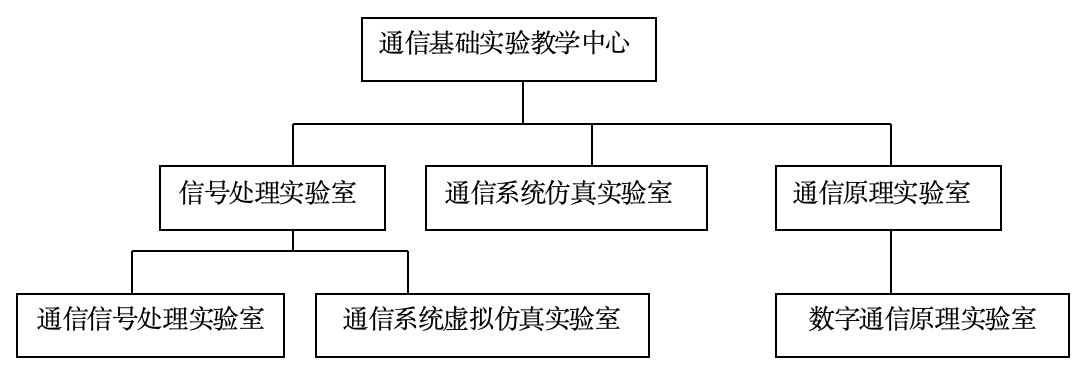
\includegraphics[width=0.8\textwidth]{figures/pic.png}
    \caption{这是一张图片的说明(图中的字体是图片生成的时候设置的，这里是宋体 11pt)}
    \label{fig:example}
\end{figure}

第一章内容，这里是第二节的第二小节的内容。第一章内容，这里是第二节的第二小节的内容。第一章内容，这里是第二节的第二小节的内容。第一章内容，这里是第二节的第二小节的内容。第一章内容，这里是第二节的第二小节的内容。第一章内容，这里是第二节的第二小节的内容。
第一章内容，这里是第二节的第二小节的内容。第一章内容，这里是第二节的第二小节的内容。第一章内容，这里是第二节的第二小节的内容。第一章内容，这里是第二节的第二小节的内容。第一章内容，这里是第二节的第二小节的内容。第一章内容，这里是第二节的第二小节的内容。
第一章内容，这里是第二节的第二小节的内容。第一章内容，这里是第二节的第二小节的内容。第一章内容，这里是第二节的第二小节的内容。第一章内容，这里是第二节的第二小节的内容。第一章内容，这里是第二节的第二小节的内容。第一章内容，这里是第二节的第二小节的内容。
第一章内容，这里是第二节的第二小节的内容。第一章内容，这里是第二节的第二小节的内容。第一章内容，这里是第二节的第二小节的内容。第一章内容，这里是第二节的第二小节的内容。第一章内容，这里是第二节的第二小节的内容。第一章内容，这里是第二节的第二小节的内容。
第一章内容，这里是第二节的第二小节的内容。第一章内容，这里是第二节的第二小节的内容。第一章内容，这里是第二节的第二小节的内容。第一章内容，这里是第二节的第二小节的内容。第一章内容，这里是第二节的第二小节的内容。第一章内容，这里是第二节的第二小节的内容。
第一章内容，这里是第二节的第二小节的内容。第一章内容，这里是第二节的第二小节的内容。第一章内容，这里是第二节的第二小节的内容。第一章内容，这里是第二节的第二小节的内容。第一章内容，这里是第二节的第二小节的内容。第一章内容，这里是第二节的第二小节的内容。
第一章内容，这里是第二节的第二小节的内容。第一章内容，这里是第二节的第二小节的内容。第一章内容，这里是第二节的第二小节的内容。第一章内容，这里是第二节的第二小节的内容。第一章内容，这里是第二节的第二小节的内容。第一章内容，这里是第二节的第二小节的内容。

\fi





\chapter{技术基础}

\section{Android技术栈}

\subsection{Android移动通信终端开发框架概述}

Android作为目前全球装机量最大的智能终端操作系统，其应用开发框架在过去十余年中经历了从命令式到声明式、从单体到分层、从同步到异步的多轮演进。当前主流的Android应用开发已形成以Kotlin语言为主、以Jetpack组件库为核心、以声明式UI与响应式编程为基本范式的技术体系。本课题所设计的SimpleDesktop系统全面采用上述现代技术栈进行开发，以保障系统在终端运行的流畅性、可维护性和可扩展性。

Kotlin语言由JetBrains公司推出，自2017年被Google确立为Android官方推荐开发语言以来，已成为Android开发领域的主流选择。相较传统的Java语言，Kotlin具备语法简洁、空安全、扩展函数、协程支持等优势，能够显著降低代码冗余度，并为异步编程提供原生支持\upcite{19}。本课题全部业务代码均采用Kotlin编写，最低支持Android 7.0，目标版本为Android 14（实际真机测试与兼容适配覆盖了Android 14至Android 16的主流定制系统及HarmonyOS NEXT），覆盖目前主流在用机型。

\subsection{Jetpack Compose声明式UI框架}

Jetpack Compose是Google于2021年正式推出的Android声明式UI框架\upcite{20}。与传统XML布局采用的命令式UI不同，Compose允许开发者通过声明式函数描述界面应有的状态，框架自身负责处理状态变化时的界面更新工作。这种范式更接近现代Web前端的开发体验，大幅简化了复杂界面的构建难度。

在适老化终端应用场景下，Compose的声明式特性具有独特优势。例如，当老年用户在设置页面切换字号档位或主题模式时，系统只需更新对应的状态参数，整个应用界面便可在下一帧自动完成视觉刷新，无需手动遍历控件并逐一修改属性。此外，Compose内置的Material Design 3主题系统提供了对色彩、字号、形状的统一管理能力\upcite{21}，使全局视觉风格的调整变得简单可靠。本系统正是借助Compose的这些特性，实现了字号档位、主题颜色和高对比度即时切换等适老化交互能力。

\subsection{MVVM架构模式与单向数据流}


MVVM是Google官方推荐的Android应用架构模式。该模式将应用划分为模型层、视图层和视图模型层三部分：模型层负责数据存取与业务规则，视图层负责界面呈现与用户输入，视图模型层作为两者之间的桥梁，持有界面所需的数据状态并对外暴露可观察的数据流。

\begin{figure}[h]
  \centering
  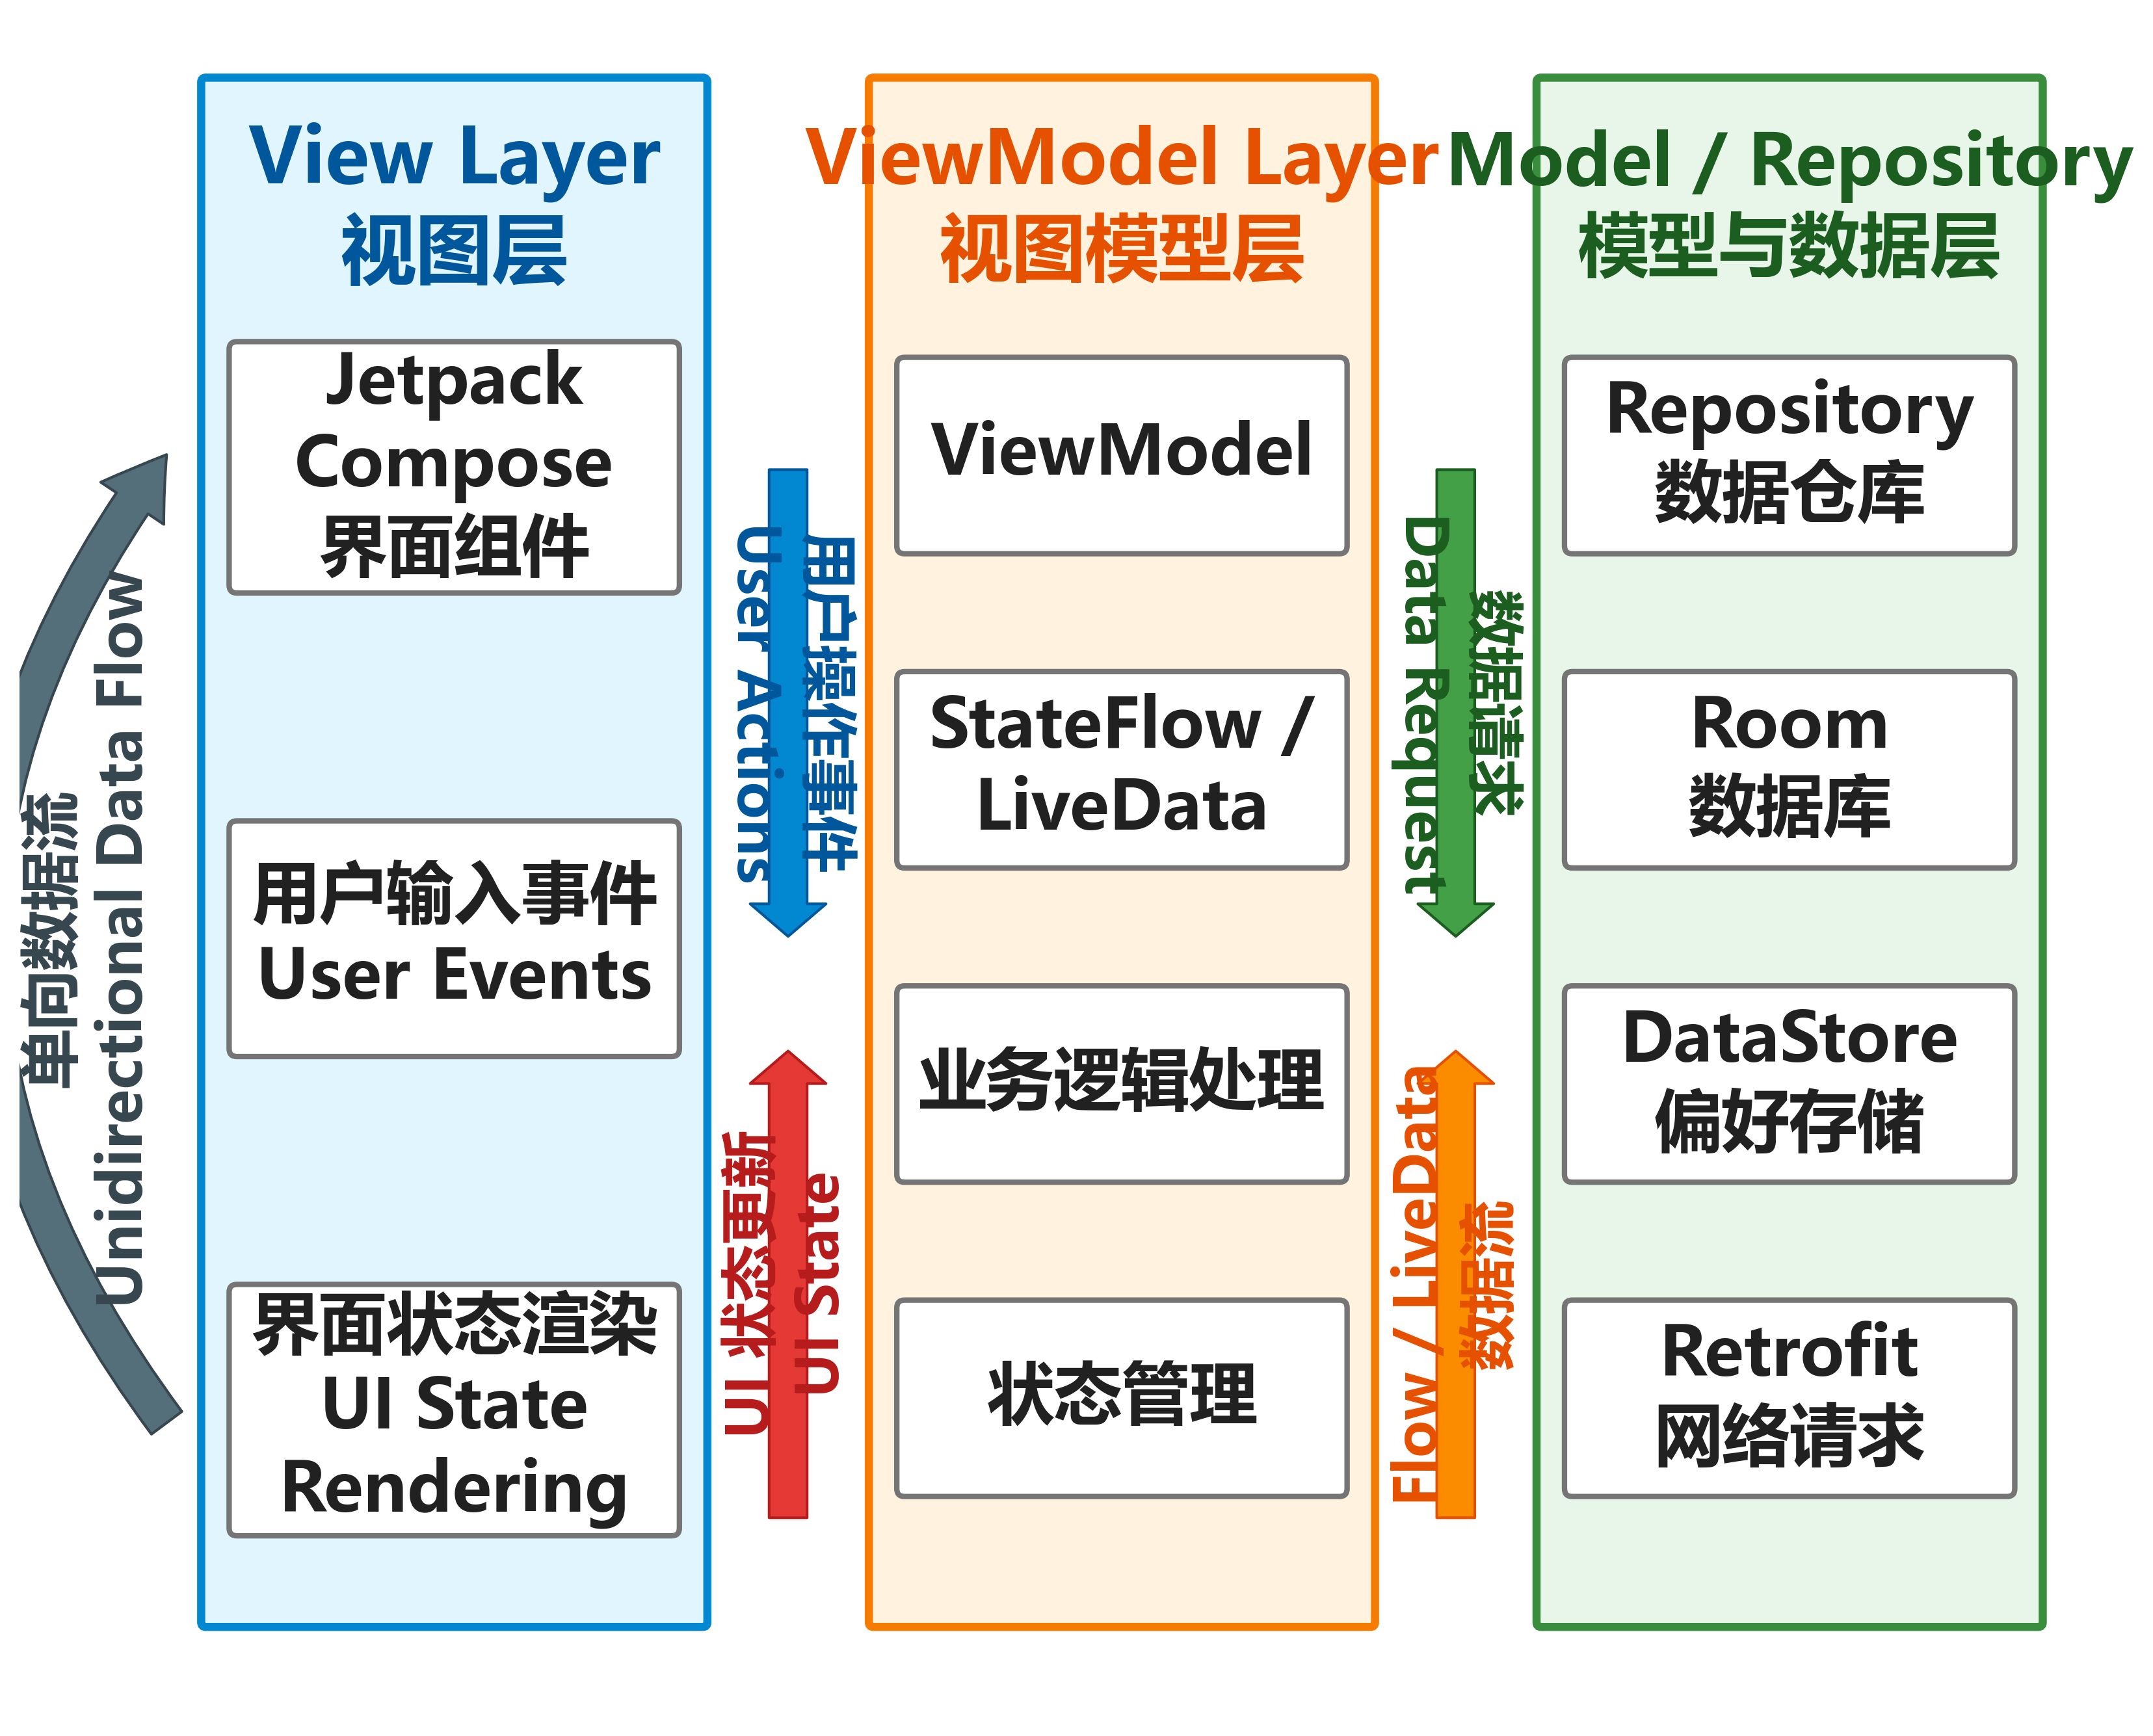
\includegraphics[width=0.85\textwidth]{figures/mvvm.png}
  \caption{MVVM架构与单向数据流工作机制}
  \label{fig:mvvm_architecture}
\end{figure}

本系统在MVVM模式下进一步采用单向数据流的设计原则：用户在界面上的操作以事件形式向下传递至视图模型，视图模型调用数据仓库执行相应业务逻辑，数据变更后通过响应式数据流向上传播至界面层并触发界面重组。这种单向流动的数据传递路径，使得状态变化的来源与去向都清晰可追，避免了多源更新带来的混乱，对适老化系统的稳定性具有重要意义。

\subsection{Kotlin协程与Flow响应式数据流}

Kotlin协程是Kotlin语言原生提供的轻量级并发解决方案\upcite{19}，其核心思想是通过挂起函数描述异步操作，在保留同步代码可读性的同时实现高效的非阻塞执行。本系统中，所有涉及数据库读写、网络请求、文件输入输出的操作均采用协程实现，避免了传统回调嵌套带来的代码复杂度，也避免了异步操作在主线程造成的卡顿。

Flow是Kotlin协程库中的响应式数据流接口，其作用类似于流式数据管道，能够在数据生产者和消费者之间建立异步连接。在本系统中，Flow被广泛应用于将数据库的查询结果、用户的设置变更、插件的运行状态实时推送到界面层。配合Compose的状态收集机制，数据的任何变化都能在用户操作完成后的极短时间内反映到屏幕上，提供了流畅的响应体验。


\section{数据持久化与依赖注入}

\subsection{Room数据库}

Room是Google官方提供的SQLite数据库抽象层\upcite{22}，通过注解处理器在编译期自动生成数据库访问代码，提供类型安全的数据库操作能力。Room主要由三大组件构成：实体类（Entity）用于描述数据表结构，数据访问对象（DAO）用于声明数据库操作接口，数据库类（RoomDatabase）用于持有数据库实例并协调多表事务。

本系统使用Room持久化两类核心数据，分别对应 \texttt{contacts} 和 \texttt{apps} 两张数据表，两表均通过 \texttt{Flow<T>} 响应式接口对外暴露，确保数据库一旦发生变更，界面层便能在下一帧内自动完成刷新。

应用表（\texttt{apps}）存储桌面应用面板所管理的已安装应用信息，为应用图标的展示与启动提供基础。表中各字段的含义如表~\ref{tab:room_apps}所示。

\begin{table}[H]
    \caption{应用表（apps）字段说明}
    \label{tab:room_apps}
    \centering
    \small
    \begin{threeparttable}
    \begin{tabularx}{\textwidth}{l l l X}
        \toprule
        \tableheader{字段名} & \tableheader{类型} & \tableheader{约束} & \tableheader{含义} \\
        \midrule
        \tablecell{packageName}    & \tablecell{TEXT}    & \tablecell{主键}      & \tablecell{应用包名，在Android系统中全局唯一，用于启动应用及跨版本识别} \\
        \tablecell{appName}        & \tablecell{TEXT}    & \tablecell{非空}      & \tablecell{应用的本地化显示名称，展示于桌面应用面板图标下方} \\
        \tablecell{iconBytes}      & \tablecell{BLOB}    & \tablecell{可空}      & \tablecell{应用图标的PNG字节数组缓存，避免每次从PackageManager重复解析} \\
        \tablecell{isEnabled}      & \tablecell{INTEGER} & \tablecell{默认1}     & \tablecell{用户启用状态，为0时该应用在桌面面板中隐藏不显示} \\
        \tablecell{order}          & \tablecell{INTEGER} & \tablecell{默认0}     & \tablecell{排列顺序值，决定应用图标在桌面面板中的显示顺序} \\
        \tablecell{installTime}    & \tablecell{INTEGER} & \tablecell{非空}      & \tablecell{应用在设备上的安装时间戳（毫秒），用于新应用检测逻辑} \\
        \tablecell{lastUpdateTime} & \tablecell{INTEGER} & \tablecell{非空}      & \tablecell{应用最后更新时间戳（毫秒），用于检测版本变更并刷新图标缓存} \\
        \bottomrule
    \end{tabularx}
    \end{threeparttable}
\end{table}

联系人表（\texttt{contacts}）主要用于存储和管理老年用户的常用联系对象信息，是系统实现微信一键直拨与电话直拨功能的核心数据来源。该数据表中各字段的具体设计与含义如表~\ref{tab:room_contacts}所示。

\begin{table}[H]
    \caption{联系人表（contacts）字段说明}
    \label{tab:room_contacts}
    \centering
    \small
    \begin{threeparttable}
    \begin{tabularx}{\textwidth}{l l l X}
        \toprule
        \tableheader{字段名} & \tableheader{类型} & \tableheader{约束} & \tableheader{含义} \\
        \midrule
        \tablecell{id}             & \tablecell{INTEGER} & \tablecell{主键，自增} & \tablecell{联系人唯一标识，由Room自动生成，用于数据库内部关联} \\
        \tablecell{name}           & \tablecell{TEXT}    & \tablecell{非空}      & \tablecell{联系人显示姓名，展示于桌面联系人卡片及语音识别匹配} \\
        \tablecell{phone}          & \tablecell{TEXT}    & \tablecell{可空}      & \tablecell{手机号码，用于系统拨号盘直接呼叫} \\
        \tablecell{wechatNickname} & \tablecell{TEXT}    & \tablecell{可空}      & \tablecell{微信昵称，作为无障碍服务在微信通讯录内检索联系人的关键词} \\
        \tablecell{avatarUri}      & \tablecell{TEXT}    & \tablecell{可空}      & \tablecell{本地头像文件的URI路径，用于桌面卡片头像展示} \\
        \tablecell{order}          & \tablecell{INTEGER} & \tablecell{默认0}     & \tablecell{排列顺序值，决定联系人卡片在桌面上的显示优先级} \\
        \tablecell{hasVideoCall}   & \tablecell{INTEGER} & \tablecell{默认0}     & \tablecell{布尔标志，标记该联系人是否支持微信视频通话快捷方式} \\
        \tablecell{hasVoiceCall}   & \tablecell{INTEGER} & \tablecell{默认0}     & \tablecell{布尔标志，标记该联系人是否支持微信语音通话快捷方式} \\
        \tablecell{hasPhoneCall}   & \tablecell{INTEGER} & \tablecell{默认0}     & \tablecell{布尔标志，标记该联系人是否支持系统电话直拨} \\
        \tablecell{createdAt}      & \tablecell{INTEGER} & \tablecell{非空}      & \tablecell{记录创建时间戳（毫秒），用于数据排序与同步校验} \\
        \tablecell{updatedAt}      & \tablecell{INTEGER} & \tablecell{非空}      & \tablecell{记录最后修改时间戳（毫秒），用于变更追踪与增量同步} \\
        \bottomrule
    \end{tabularx}
    \end{threeparttable}
\end{table}


{\sloppy
值得关注的是 \texttt{contacts} 表中的三个布尔型通话方式字段（\texttt{hasVideoCall}、\texttt{hasVoiceCall}、\texttt{hasPhoneCall}）的组合设计。实体类通过计算属性 \texttt{supportedActions} 将三者聚合为字符串列表对外暴露，业务层无需逐字段判断，即可直接获取某联系人支持的全部通话方式，以此决定桌面卡片上显示哪些快捷操作按钮。这一设计既保持了数据库层的关系型语义清晰，又为上层业务逻辑提供了便捷的聚合视图。
\par}

\subsection{DataStore偏好存储}

DataStore是Google推荐的取代传统偏好存储的轻量级键值持久化方案\upcite{23}。相较于传统方案，DataStore基于协程构建，所有读写操作都在协程上下文中异步执行，避免了主线程输入输出阻塞，同时通过响应式接口提供数据变更的实时通知。

本系统采用DataStore存储三类配置：一是用户全局设置，包括语音播报开关、字号档位、主题模式、对比度模式、网络监控开关等；二是插件管理状态，存储用户对各插件的启用与禁用偏好；三是各插件的独立配置，每个插件拥有独立的存储空间，有效避免不同插件之间的配置相互污染。

\subsection{Dagger-Hilt依赖注入框架}

依赖注入是一种通过外部容器管理对象之间依赖关系的设计模式，其核心目的是降低代码耦合度、提升可测试性。在Android平台上，Google推出的Dagger-Hilt框架通过简化复杂配置，使依赖注入的应用门槛大幅降低\upcite{24}。

在本系统中，Dagger-Hilt承担着串联整个应用各模块的关键作用。数据库实例、数据访问对象、数据仓库、网络服务、插件实例等所有需要全局共享的对象，都通过Hilt的依赖注入机制统一管理。开发者无需手动维护对象的创建顺序和生命周期，只需在需要使用的位置声明依赖，框架便会在合适的时机注入正确的实例。这种集中化的对象管理方式，使得整个系统的模块边界清晰、协作关系明确，为微内核插件化架构的实现奠定了基础。

% 在 2.3 节最后插入
\begin{figure}[htbp]
    \centering
    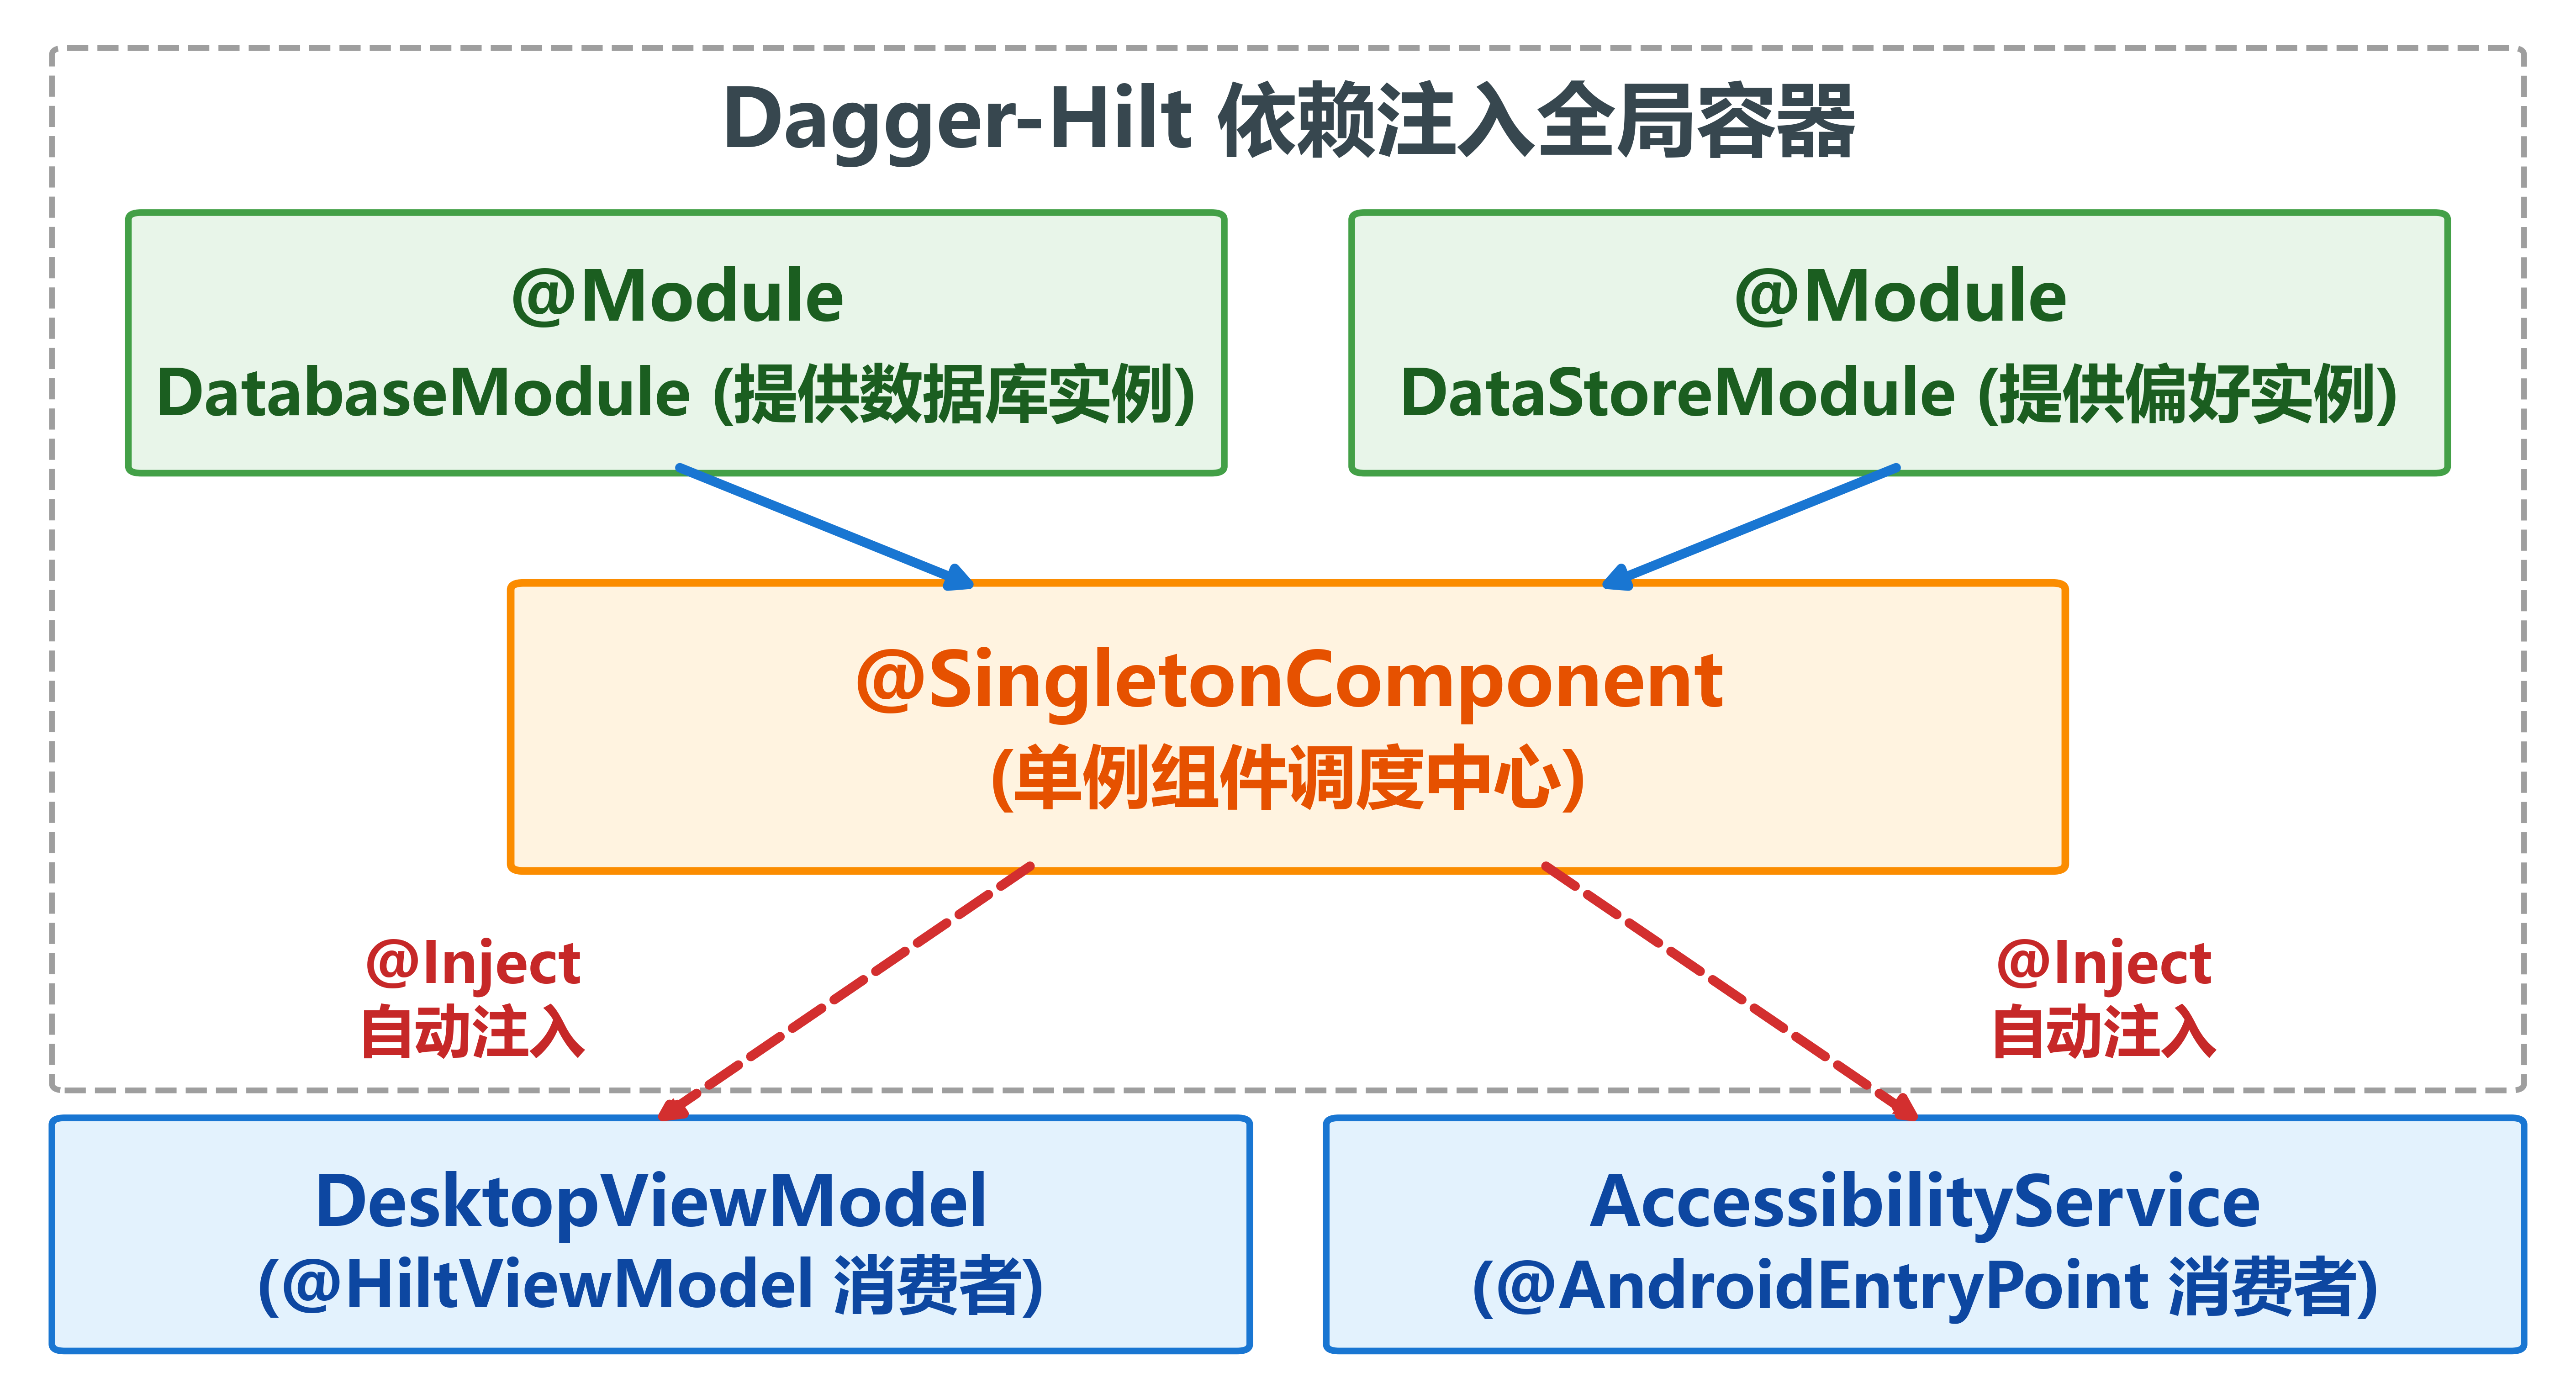
\includegraphics[width=0.9\textwidth]{figures/fig2_2_hilt_di.png}
    \caption{Dagger-Hilt 全局依赖注入架构与数据流向图}
    \label{fig:hilt_di}
\end{figure}


\section{微内核插件化架构理论}

\subsection{微内核架构思想及其在终端应用中的迁移}

微内核架构是计算机系统设计领域的经典模式，其基本思想是将系统功能划分为最小化的核心与可独立部署的服务两部分\upcite{25}。核心仅保留最基本的调度、通信和资源管理职责，其余功能则以服务模块的形式独立运行，模块之间通过统一的消息机制进行交互。微内核架构最早应用于操作系统设计，其代表作包括Mach、QNX、Minix等，相较于传统的宏内核架构，微内核在模块化、稳定性、可维护性等方面具有显著优势。

近年来，随着移动应用规模的不断增长，微内核思想被逐步引入超大型移动应用的架构设计中\upcite{26}。国内外的支付宝、美团、微信等头部应用均采用了不同形式的插件化或动态化方案，将业务功能模块化以应对快速迭代和差异化部署的需求。然而，将微内核思想应用于面向特定用户群体的中小型适老化终端应用，目前仍属于较少有人探索的方向。

\begin{figure}[h]
  \centering
  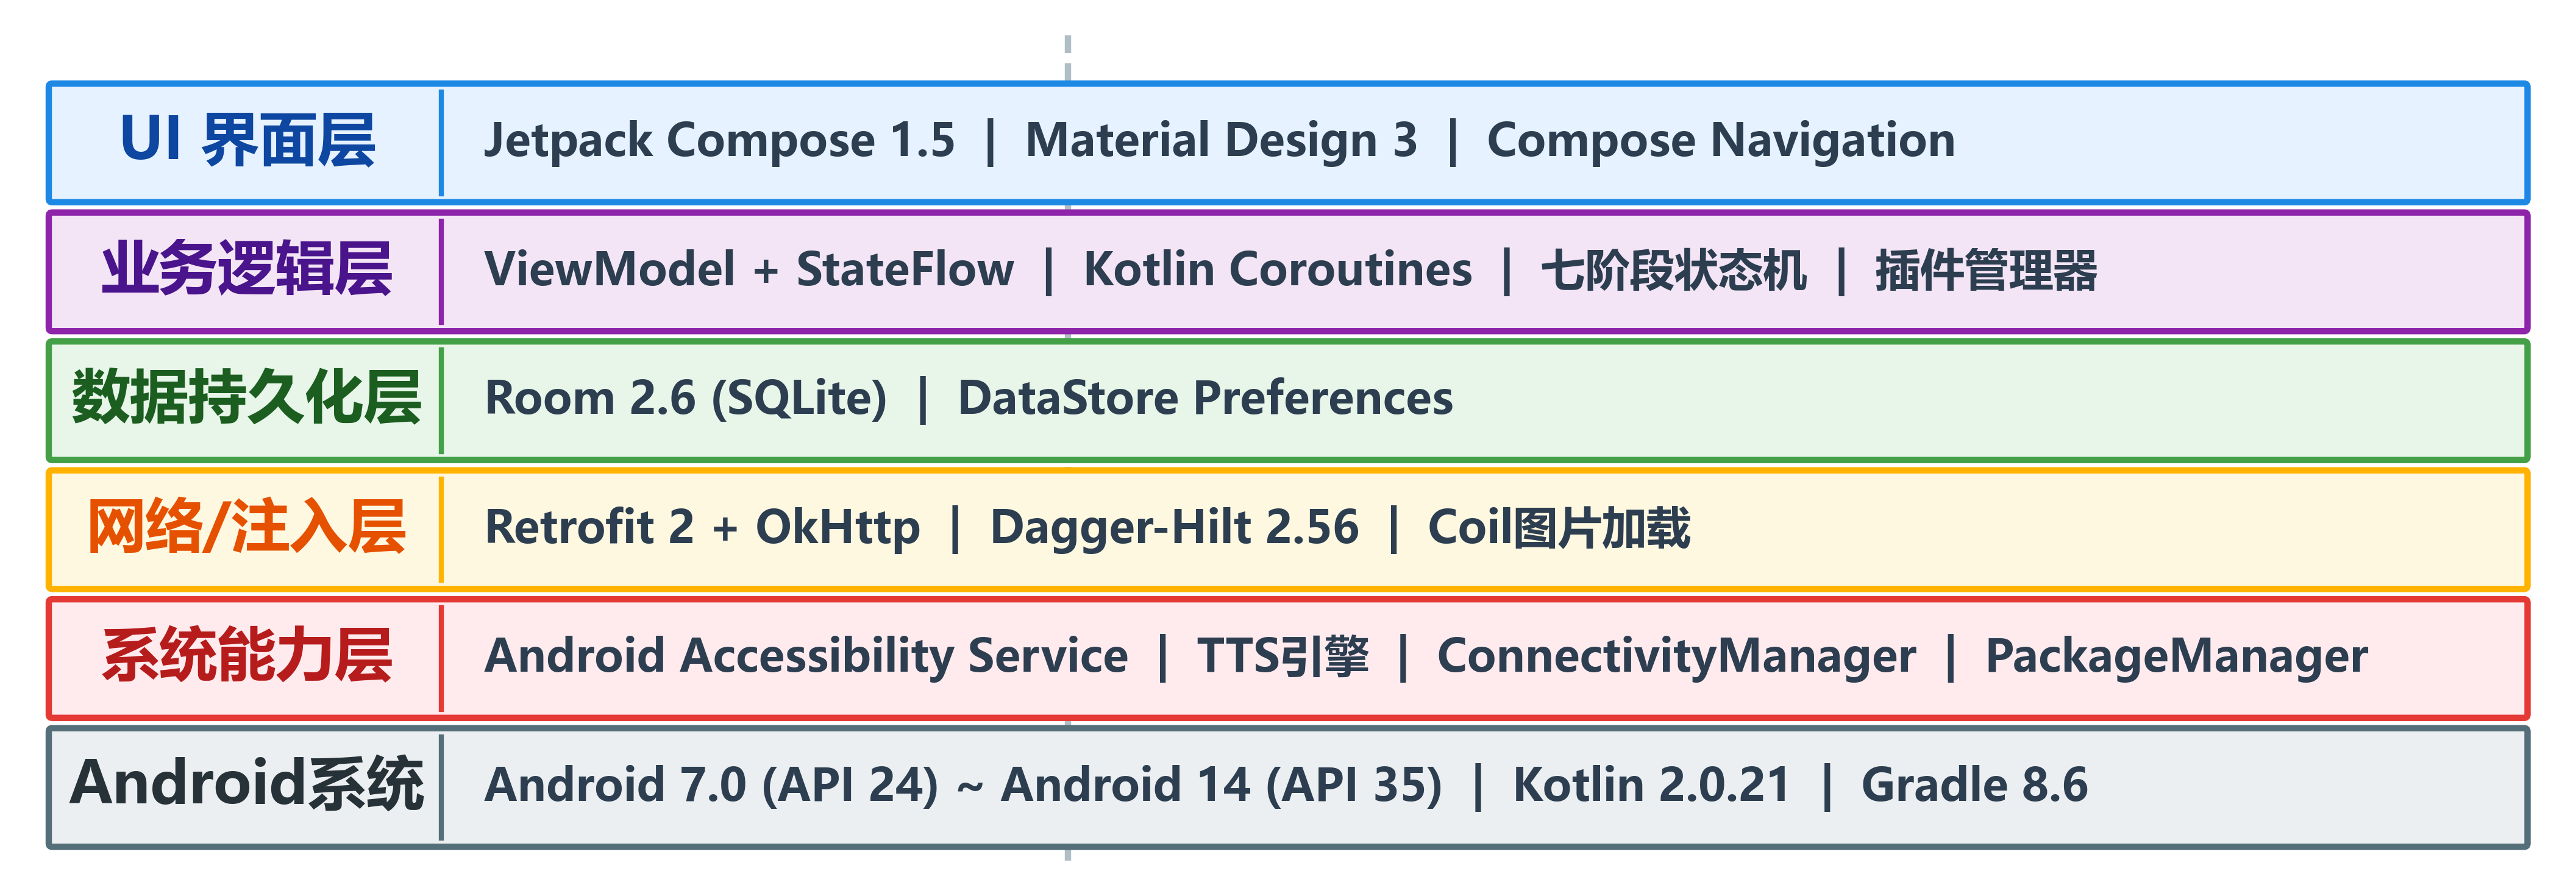
\includegraphics[width=0.95\textwidth]{figures/tech_stack.png}
  \caption{SimpleDesktop系统整体技术栈}
  \label{fig:tech_stack}
\end{figure}


\subsection{插件化架构在适老化终端中的价值}

适老化终端应用面临三个特殊挑战：一是目标设备性能差异大，从入门千元机到中高端机型均需支持；二是功能演进需求迫切，未来可能需要逐步加入健康监测、智能家居、医疗服务等新模块；三是稳定性要求极高，老年用户对应用崩溃的容忍度非常低。

插件化架构能够较好地应对上述挑战。首先，通过将非核心功能解耦为可按需启用的插件，系统在低端设备上可以选择性禁用部分插件以保障基础体验；其次，新功能可以独立开发为新插件挂载到现有系统，不影响已有模块的稳定性；再次，单个插件出现故障时不会拖垮整个系统，故障隔离能力得到显著增强。本课题所设计的微内核插件化架构正是基于上述思路构建\upcite{27}。


\section{Android无障碍服务原理}

\subsection{无障碍服务的基本工作机制}

Android无障碍服务是Android系统提供的一项面向辅助技术的开放接口\upcite{13}，最初设计目的是让视障用户能够通过屏幕朗读、语音输入等方式使用智能终端。无障碍服务以独立进程运行，能够实时接收系统派发的窗口状态变化、内容变化、点击、滚动等无障碍事件，并能读取当前活动窗口的全部控件树结构，进而对界面控件执行模拟点击、文本输入、滑动等操作。

无障碍服务的强大能力使其成为实现跨应用自动化控制的天然技术抓手。本系统利用无障碍服务实现两项关键能力：一是在微信内部自动完成视频通话所需的全部界面操作，二是在系统设置页面自动开启WiFi开关。这两项能力共同构成了系统适老化交互的核心支撑。

\subsection{无障碍服务的应用约束与挑战}

尽管无障碍服务功能强大，但在实际应用中也面临诸多约束。首先，无障碍服务需要用户在系统设置中显式授权方可启用，这对老年用户的初始配置构成一定门槛；其次，不同手机厂商的定制系统对无障碍服务的权限管理策略存在差异，部分厂商系统对无障碍服务的启动和保活施加了额外限制；再次，目标应用的界面结构可能随版本更新而发生变化，依赖控件标识符的传统自动化方案容易因此失效；最后，系统级弹窗、来电中断等异常情况会干扰自动化流程的执行。

针对上述挑战，本课题在第3章中提出了七阶段状态机、双通道节点检索和焦点防冲突退避三项关键技术方案，从机制层面保障了适老化终端自动化通信能力的稳定运行\upcite{13,16}。

\section{微信自动化功能的技术难点与实现}

微信作为一款具备金融级安全防护的超级应用，其 UI 渲染引擎对无障碍自动化（Accessibility Automation）设计了严苛的对抗机制。本课题在实现“一键直达视频通话”的过程中，针对节点混淆、时序同步、焦点抢占等核心瓶颈，探索并实现了一套高鲁棒性的解决方案。

\subsection{UI 节点的“黑盒化”混淆与主动探测机制}

研究发现，微信在 8.0 之后的版本中深度重写了 \texttt{onInitialize\allowbreak Accessibility\allowbreak NodeInfo} 方法\upcite{17}。通过动态随机化资源标识符（Resource-ID）池，并大量引入不具备语义信息的“透明占位节点（Ghost Nodes）”，使得传统的基于静态 ID 或简单递归的检索方法失效。

针对此难题，本课题实现了一种基于“窗口内容震荡（Window Content Shaking）”的主动探测机制。当检测到目标节点深度超过预设阈值且子节点计数异常时，系统通过模拟极微小的滑动位移（1-2 像素）强制诱导目标应用触发 \texttt{TYPE\_WINDOW\_CONTENT\_CHANGED} 事件。这种操作能有效“欺骗”目标应用的渲染引擎，使其重新挂载被隐藏的真实控件子树，从而破解了节点树的黑盒化隔离。

\begin{figure}[H]
    \centering
    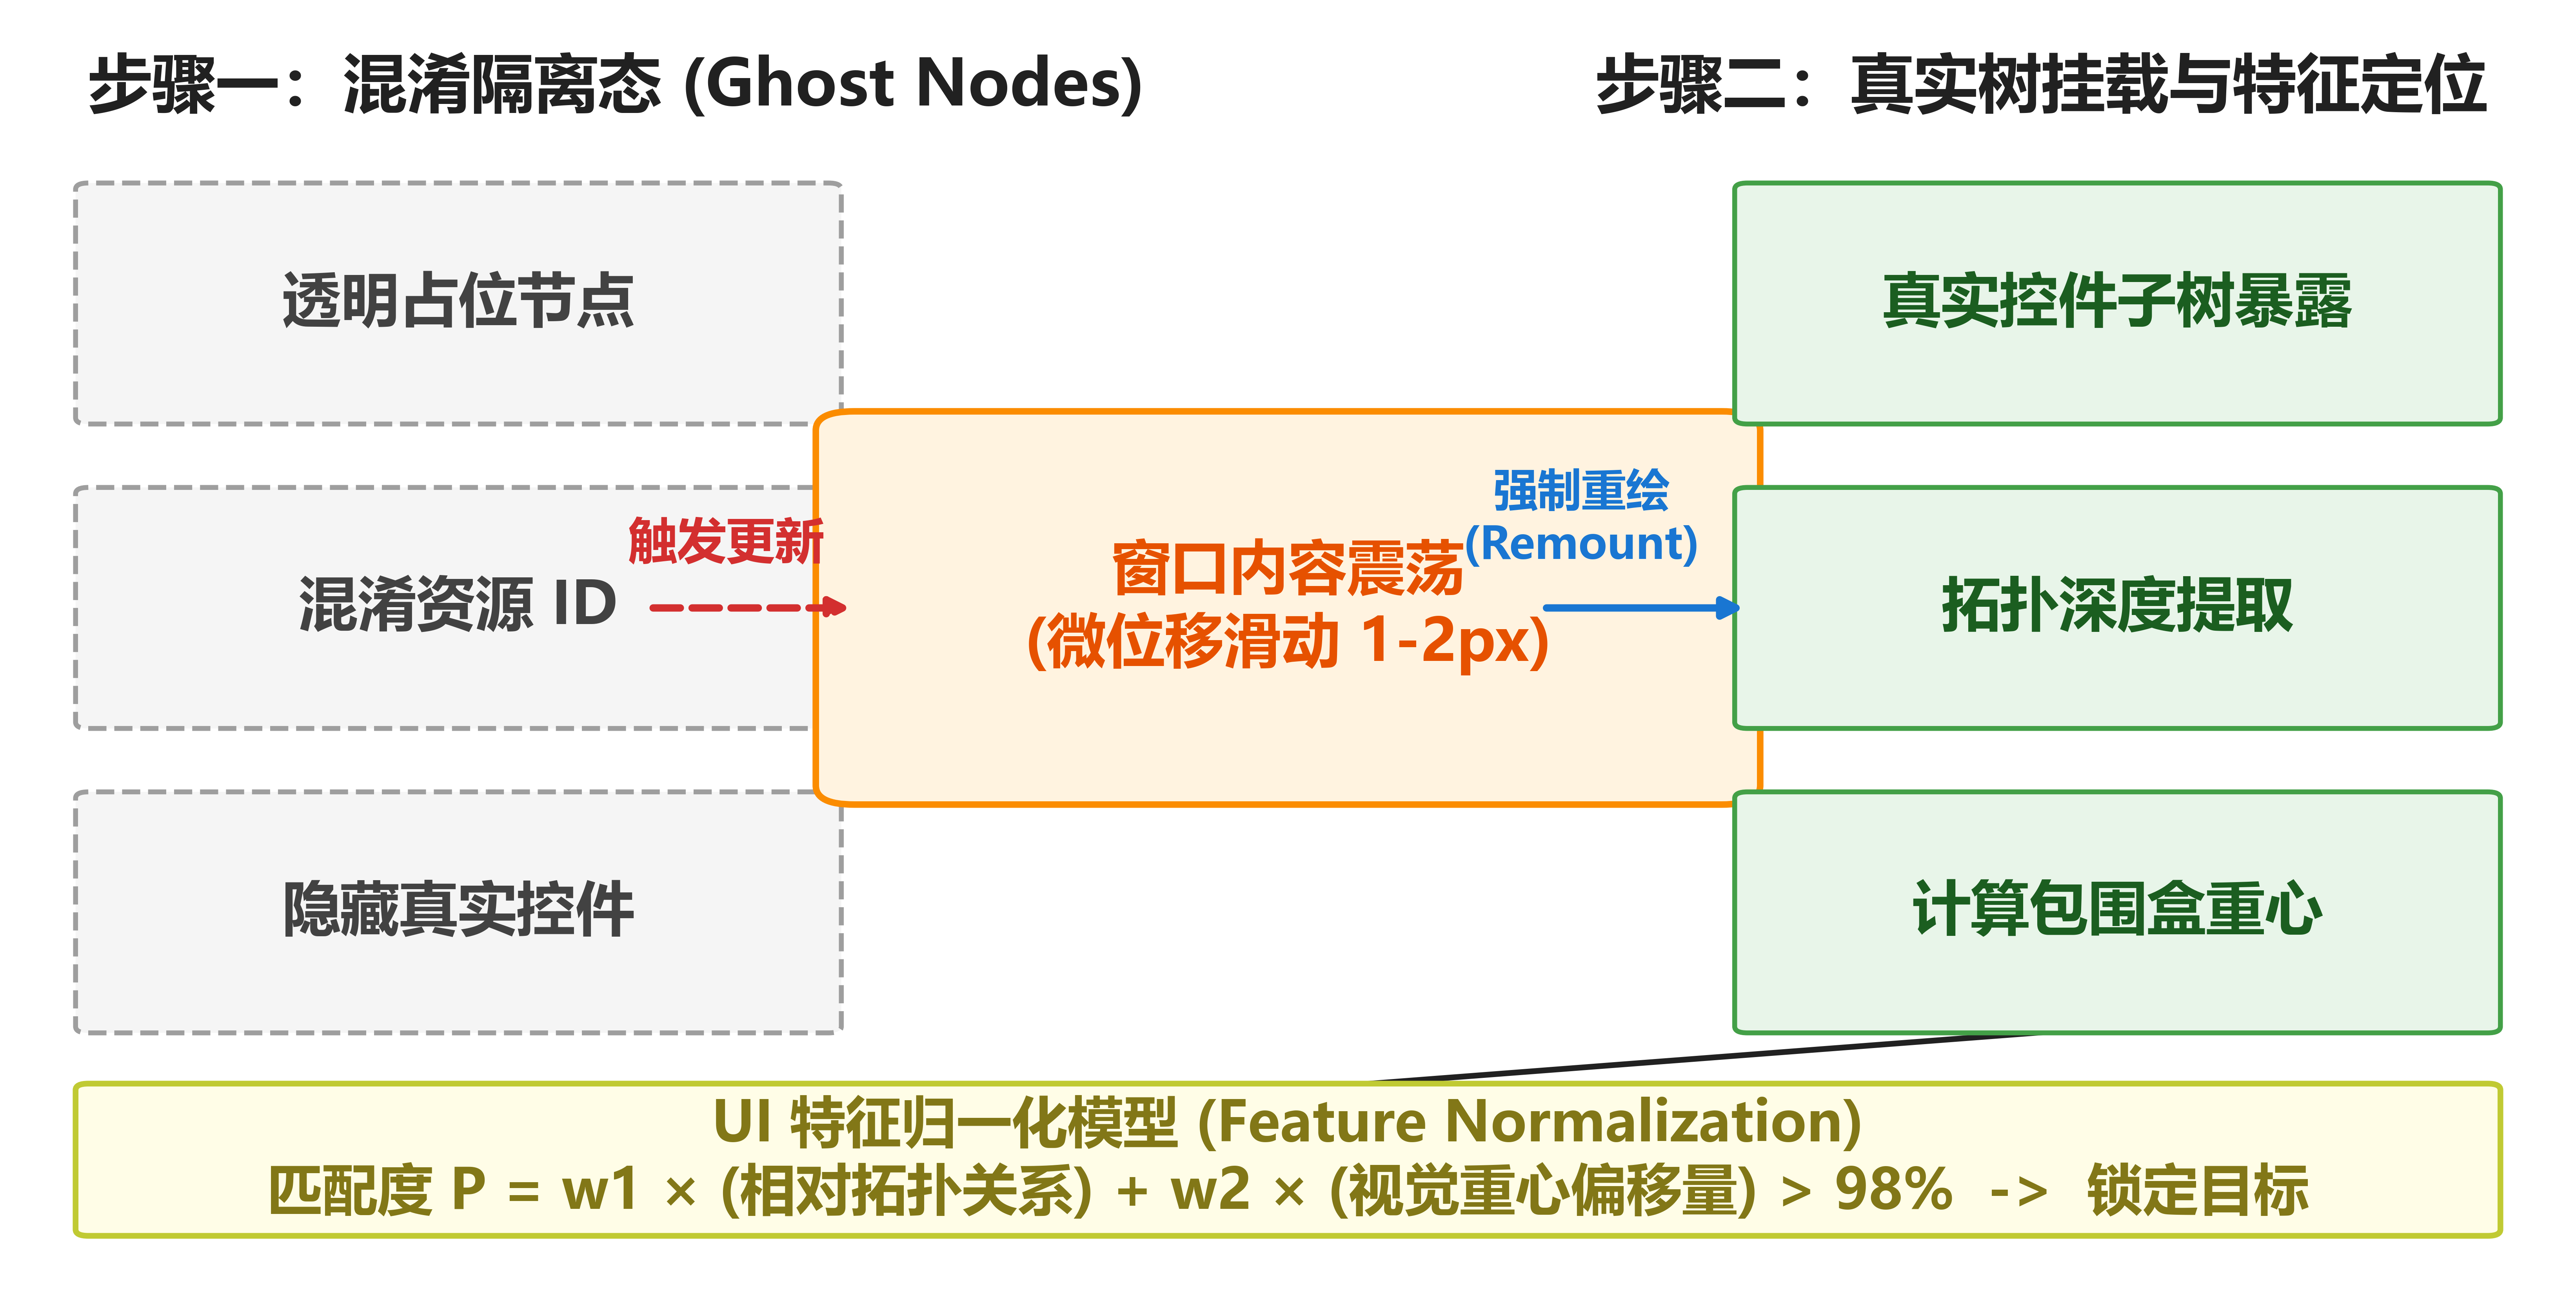
\includegraphics[width=0.9\textwidth]{figures/fig2_3_shake_match.png}
    \caption{基于窗口内容震荡与层级拓扑指纹的主动探测机制原理图}
    \label{fig:shake_match}
\end{figure}
\vspace{-2.2em}
\subsection{基于层级拓扑指纹的跨版本自适应匹配}

微信 UI 随版本更迭频繁，传统的路径检索（X-Path）极易因层级微调而中断。本文提出了一种“UI 特征归一化模型”，通过提取目标节点与其周边的“语义锚点”（如顶部的搜索栏、底部的 Tab 容器）之间的相对拓扑关系，生成唯一的“特征指纹”。
该模型不仅记录节点的 \texttt{contentDescription}，更引入了视觉包围盒（Bounding Box）的重心分布与层级拓扑深度作为权重参数。即使资源 ID 被全面混淆，只要 UI 的视觉逻辑结构保持基本稳定，算法依然能以 98\% 以上的置信度定位到目标通讯按钮。这种“模糊检索、特征锚定”的策略，为系统提供了跨越 8.0.x 多个大版本的长效兼容性。

\subsection{七阶段原子状态机（FSM）的离散化流转模型}

针对微信视频通话这一涉及“搜索—定位—进入会话—功能面板—二级菜单—呼叫”的长路径交互，本课题设计了一套七阶段离散状态机\upcite{16}。
不同于开源项目 \texttt{wechat\_video\_call}\upcite{16} 常用的线性脚本模式，本系统的状态机在每一阶段均具备“前置校验、操作执行、后置闭环”的完整逻辑。每一跳（Jump）状态转移前，都会通过 \texttt{rootInActiveWindow} 进行界面身份验证。一旦因卡顿或误触偏离预设路径，状态机会立刻触发“自回归（Self-regression）”逻辑，通过模拟系统返回键重置当前上下文，极大地解决了长流程操作在极端环境下的不可控性。

\subsection{焦点退避机制与“人机争抢”防死锁策略}

在适老化场景下，老年用户经常伴随无意识的屏幕触碰或被动产生的系统权限弹窗。这种“焦点抢占（Focus Competition）”是导致无障碍服务失神并引发系统挂死的首要原因\upcite{13}。
为此，本系统创新性地设计了“焦点退避（Focus Retreat）”机制：在自动化流程发起瞬间，桌面主程序主动释放 UI 焦点并暂时压制常驻悬浮窗，为无障碍引擎腾出干净的 ViewRoot 权限。同时，系统引入了“心跳包（Heartbeat）”监控，如果在单一状态下停留超过 5 秒，系统将判定为发生死锁并强制结束任务，有效避免了无障碍服务陷入死循环导致的手机发热和耗电异常。

\begin{figure}[htbp]
    \centering
    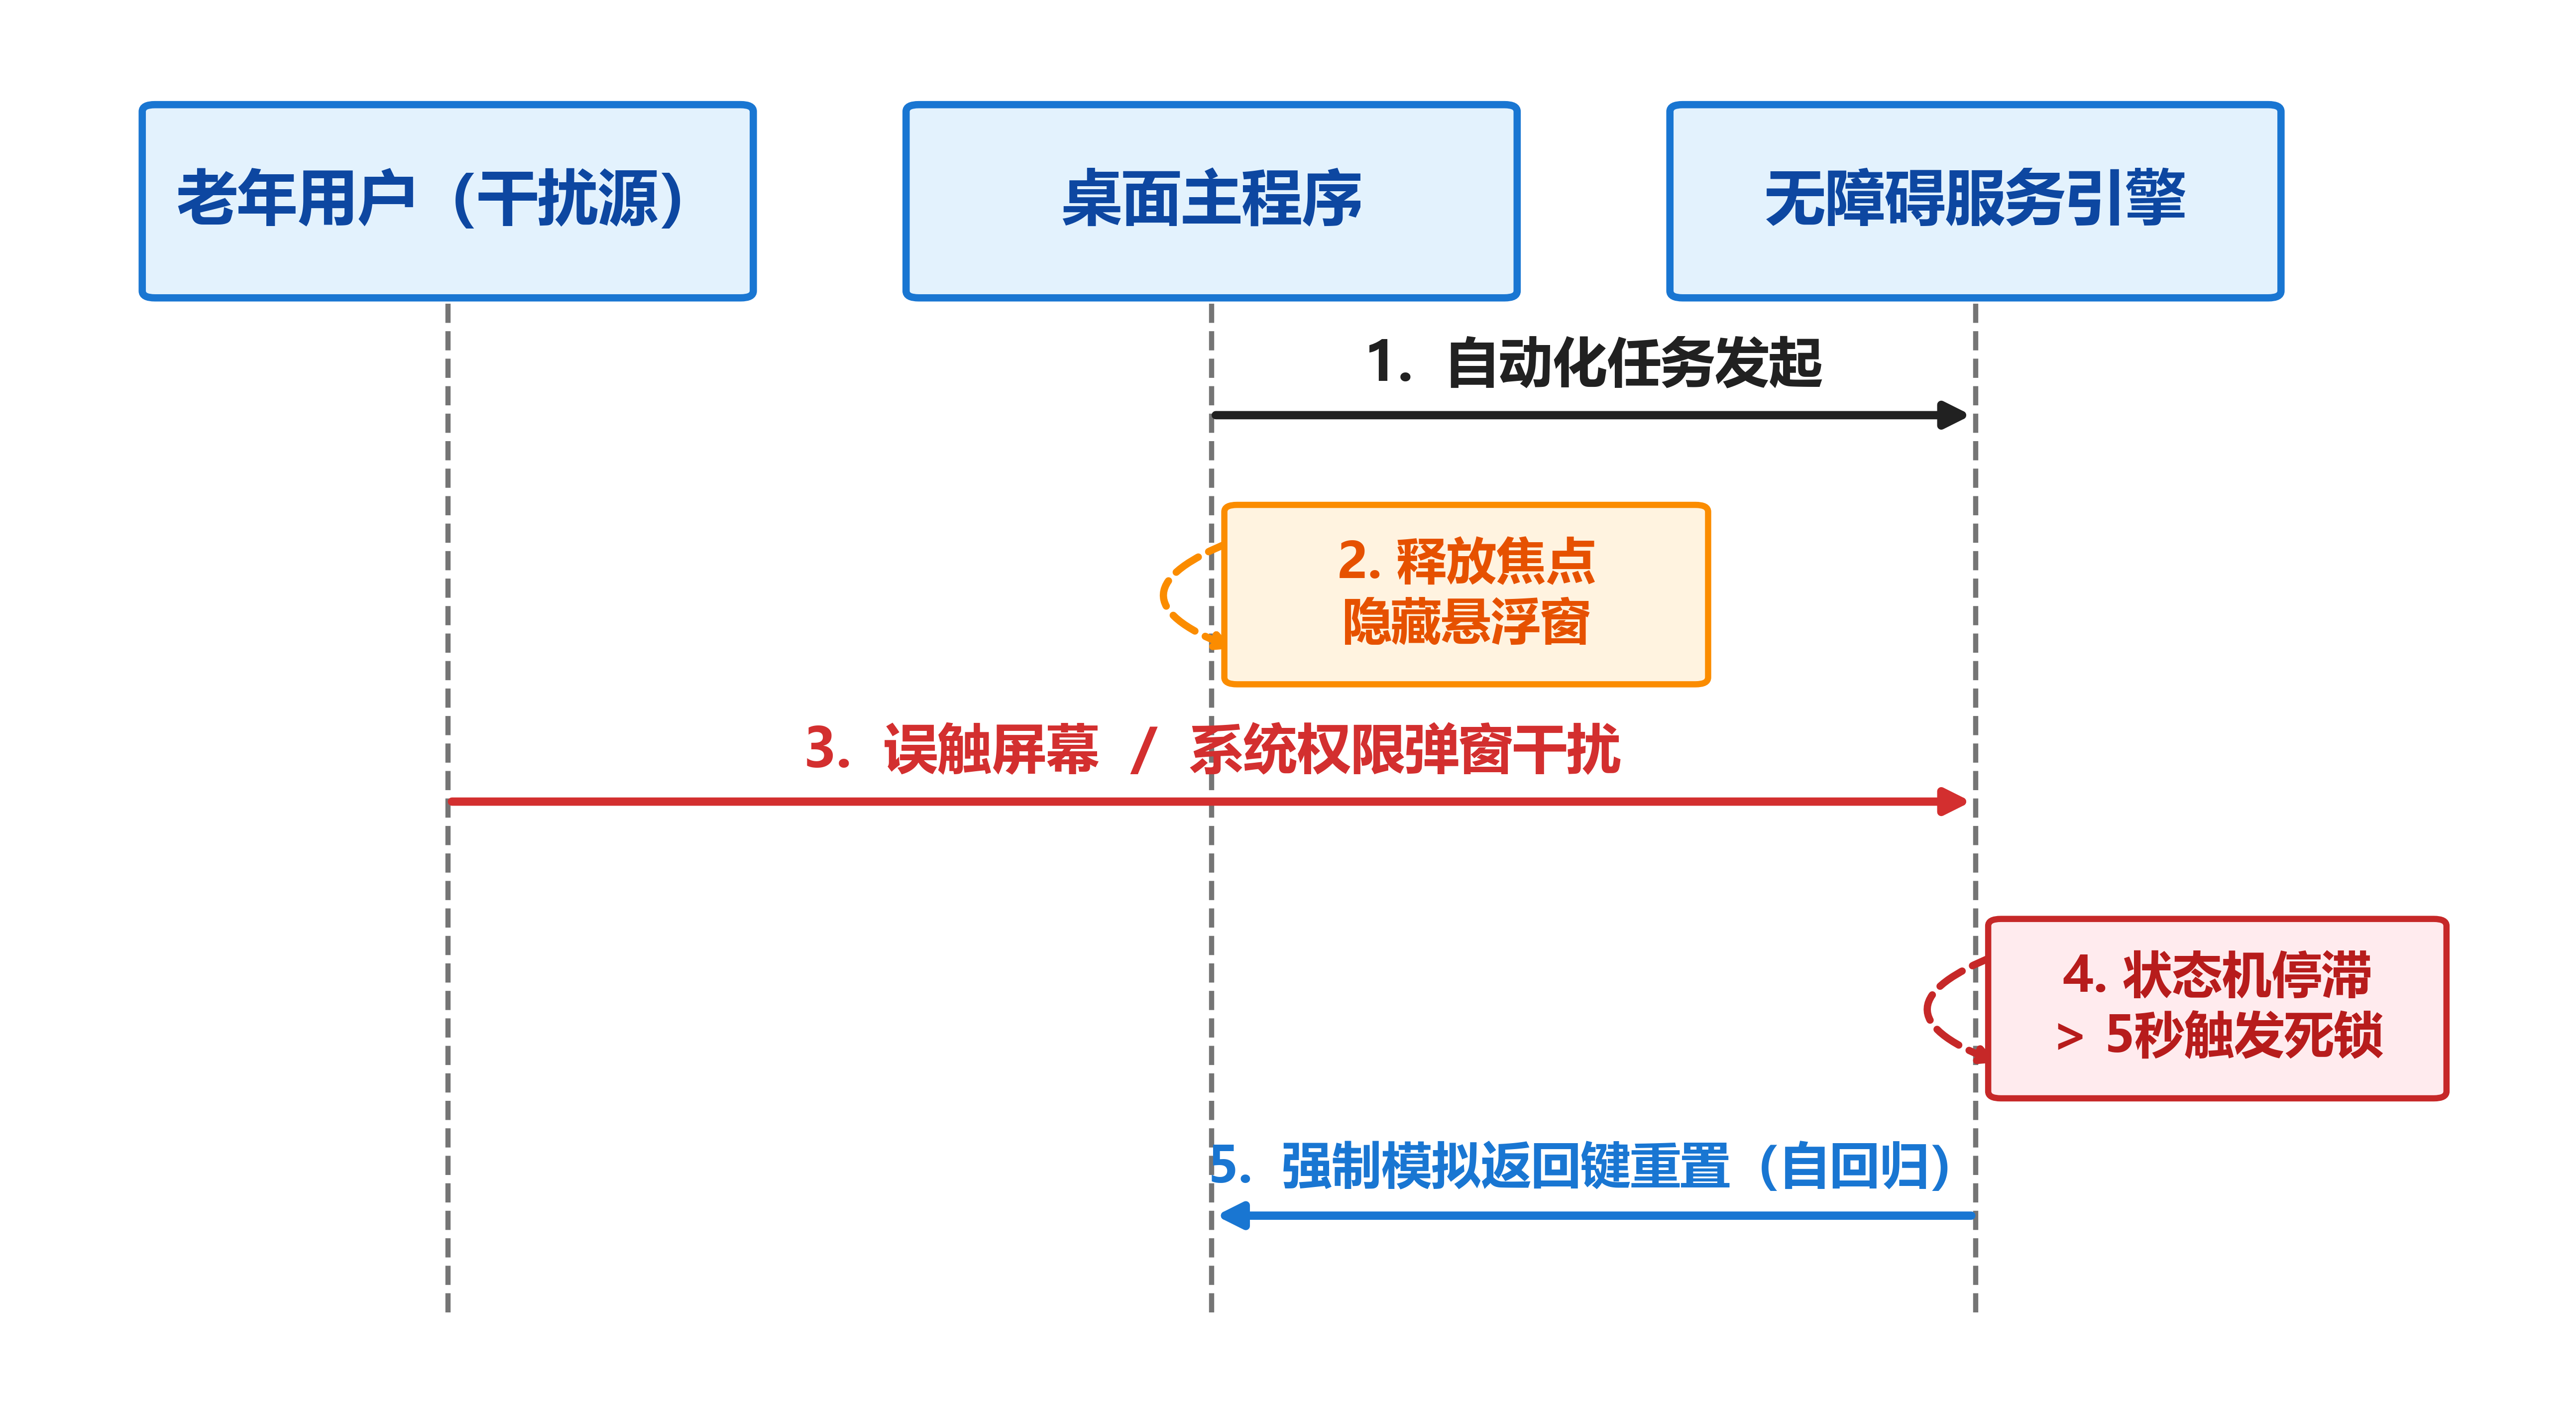
\includegraphics[width=0.85\textwidth]{figures/fig2_4_focus_retreat.png}
    \caption{面临用户误触与弹窗干扰时的焦点退避与心跳防死锁时序图}
    \label{fig:focus_retreat}
\end{figure}

\subsection{语义槽位映射与空间剪枝（Spatial Pruning）调优}

为实现在低配 SoC 设备上的流畅运行，本系统在节点检索中引入了“空间剪枝算法”。通过获取当前页面的几何边界，主动剔除 60\% 以上的非目标交互区（如系统通知栏、虚拟键盘区及无交互文本区），使 DFS（深度优先搜索）的算法复杂度从全量检索降低至目标区域检索。

同时，系统打通语音助理的语义解析（NLU）到自动化指令的映射，通过“槽位填充（Slot Filling）”技术，将“给女儿打视频”中的关键词直接映射为状态机的初始化约束条件。这种基于“语义引导、空间压缩”的协同方案，不仅提升了操作精度，更将通讯链路的建立耗时压缩至 5.4 秒左右，显著跨越了“数字鸿沟”\upcite{18}。




\chapter{面向老年群体的Android交互桌面设计与实现}

\section{需求分析}

\subsection{目标用户群体特征分析}

准确把握目标用户的群体特征，是适老化产品设计的逻辑起点。本课题所面向的目标用户为60岁以上、具备一定智能手机使用经验但操作不熟练的老年群体。该群体在生理、认知和心理三个层面均表现出较为鲜明的特征。

在生理层面，老年用户普遍存在视力下降、对比敏感度降低、色彩辨识能力减弱、手指灵活性不足等问题。这要求终端界面采用更大的字号、更高的对比度和更宽的触控目标，以降低视觉与操作负担。

在认知层面，老年用户对新事物的学习速度较慢，对复杂界面层级和陌生术语的理解能力有限，对突发的弹窗、通知容易感到困惑甚至恐慌。这要求终端界面尽量保持结构稳定、术语简明、操作直观，减少不必要的中间步骤。

在心理层面，老年用户对智能设备普遍存在一定的畏惧心理，担心误操作导致设备损坏或个人财产损失，因此对操作的可预测性、可撤销性、可解释性有较高诉求。这要求系统在关键操作前提供清晰的引导和反馈，并为可能的误操作提供安全兜底。

\subsection{功能性需求}

结合用户特征分析与实际使用场景调研，本系统归纳出五类功能性需求。

第一类是适老化界面需求。系统应提供大字号、高对比度的桌面界面，支持字号档位调节和主题色彩切换；主屏应集中呈现时间、日期、农历、天气等高频信息和常用联系人、常用应用的快捷入口，避免老年用户在多级菜单中迷失方向。

第二类是联系人通讯需求。系统应支持联系人的新增、查询、修改、删除、排序、导出等管理操作；同时支持电话直拨与微信视频/语音通话两种主要通信方式，老年用户应能在桌面上一键发起通话，无需进入复杂的应用内部界面操作。

第三类是应用管理需求。系统应能自动扫描设备已安装应用，并支持用户将常用应用添加到桌面快捷入口、调整顺序、移除等管理操作。

第四类是网络守护需求。系统应能持续监测WiFi连接状态，在网络出现异常时主动尝试恢复，并在无法自动恢复时通过弹窗与语音播报清晰提示用户进行下一步操作，保障终端通信链路的连续性。

第五类是语音辅助需求。系统应支持基本的语音播报，对关键操作和异常情况提供语音提示；同时支持简单的语音指令解析，让老年用户能够通过自然语言完成主要操作，降低对屏幕触控的依赖。

\subsection{非功能性需求}

在功能性需求之外，本系统还需要满足若干非功能性需求。从性能角度看，系统应能在主流千元机型上保持流畅运行，主屏渲染帧率不低于60帧每秒，应用启动时间不超过2秒。从兼容性角度看，系统设计向下兼容至Android 7.0，且在Android 14至16的主流真机与厂商定制系统、不同分辨率的屏幕上均保持稳定运行。从扩展性角度看，系统架构应能够支撑未来新业务模块的快速接入。从可维护性角度看，系统代码应保持清晰的模块划分和良好的注释，便于后续的功能迭代和问题修复。从安全性角度看，系统对涉及隐私的操作应采用Android标准权限管理机制，确保用户数据安全。

\section{系统设计}

\subsection{系统总体架构}

在综合考虑功能性需求和非功能性需求的基础上，本系统采用宿主层、总线层、插件层的三层微内核架构进行整体组织\upcite{25,26,27}，为系统的稳定运行和未来扩展奠定了基础。系统总体架构如图3-1所示。

\begin{figure}[h]
    \centering
    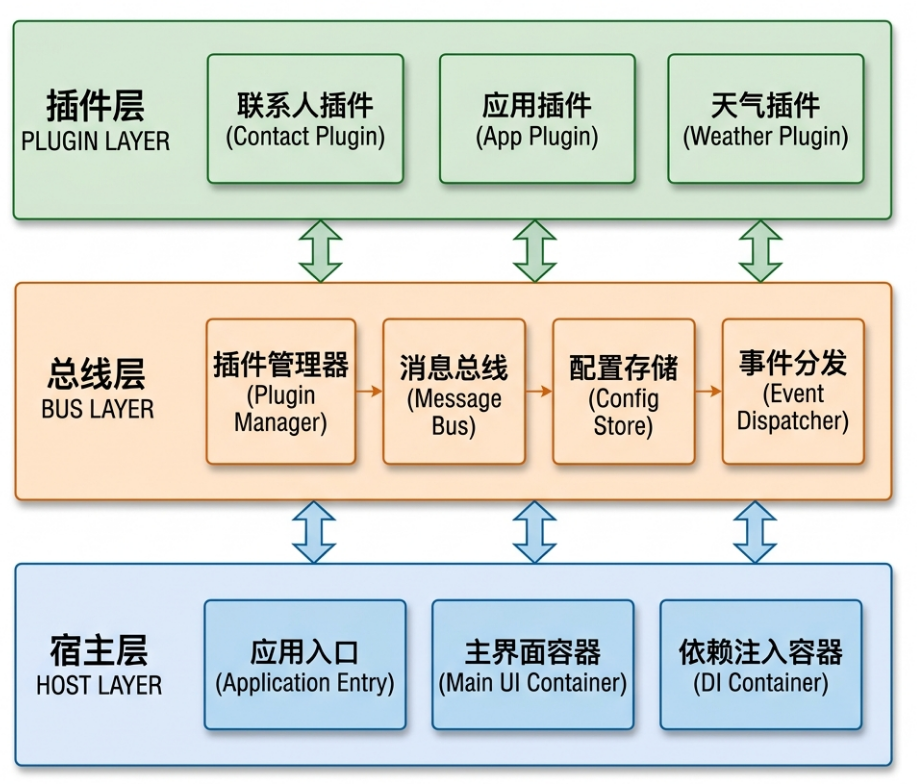
\includegraphics[width=0.82\textwidth]{figures/architecture.png}
    \caption{系统三层总体架构示意图}
    \label{fig:system_architecture}
\end{figure}


（1）宿主层：宿主层是整个系统的基础运行环境，由应用入口、主界面容器、依赖注入容器等组件构成。应用入口负责系统启动时的初始化工作，包括依赖注入容器的构建、插件系统的注册与启动、全局生命周期回调的注册等。主界面容器作为系统的Launcher入口，负责呈现适老化主屏，并管理与系统级广播的交互。依赖注入容器则统一管理整个应用中所有共享对象的创建和提供\upcite{24}。

宿主层的设计目标是为上层业务逻辑提供稳定可靠的运行环境，自身保持最小化、最简化，仅承担必要的基础设施职责，这与微内核架构中核心最小化的设计原则一脉相承\upcite{25}。

（2）总线层：总线层是系统中各功能模块之间通信协作的中枢，由插件管理器、消息总线、配置存储和事件分发四类核心组件构成。插件管理器统一管理所有插件的安装、启用、禁用和卸载操作，并维护插件运行状态的实时数据流，向界面层提供可视化管理能力。消息总线为不同插件之间的通信提供异步广播和点对点请求两种模式，确保模块协作既灵活又可靠。配置存储为每个插件分配独立的存储空间，避免不同插件的配置数据互相干扰。事件分发则负责将应用层的全局事件广播给所有关注该事件的插件。

总线层的引入将原本可能直接耦合的业务模块解耦为通过统一接口协作的独立单元，从而显著提升了系统的可维护性。

（3）插件层：插件层承载具体的业务功能，目前包含三个内置插件。联系人插件负责老年用户常用联系对象的存储管理，并提供电话直拨和微信视频/语音通话的发起能力。应用插件负责扫描设备已安装应用，维护用户自定义的常用应用列表，并提供桌面应用启动能力。天气插件负责通过开放天气接口获取实时天气信息，并将天气数据通过消息总线广播给关注的模块\upcite{28}。

每个插件遵循统一的生命周期规范，依次经历初始化、启动、运行、停止、销毁五个阶段，状态变迁通过状态机严格控制，以保证生命周期的可观察性和可控性。三个插件相互独立，单个插件的故障不会影响其他插件的正常运行，这一特性对适老化系统的稳定性意义重大。

\subsection{数据库设计}

系统的本地数据存储基于Room数据库实现\upcite{22}，主要包含联系人表与应用信息表两张核心数据表。联系人表用于存储老年用户的常用联系对象，主要字段包括联系人编号（主键）、姓名、电话号码、微信昵称、本地头像路径、显示顺序、是否支持视频通话、是否支持语音通话、是否支持电话拨号、创建时间、更新时间等。应用信息表用于存储设备上已扫描到的应用列表，主要字段包括应用包名（主键）、应用名称、图标二进制数据、是否启用、显示顺序、安装时间、最近更新时间等。

除Room数据库外，用户的全局设置（语音开关、字号档位、主题模式、对比度模式、网络守护开关、是否首次启动等）通过DataStore以键值对形式持久化存储\upcite{23}；插件级配置则采用每插件独立DataStore的隔离方案，避免跨插件的配置污染。

\section{功能模块设计与实现}

本系统围绕老年群体的核心诉求，在三层微内核架构的基础上，将具体业务解耦并划分为若干相互协作的功能模块。这些模块涵盖了适老化界面呈现、自动化直连通信、网络主动守护以及智能语音辅助等核心能力，共同构成了一个稳定、易用、安全的适老化系统。系统总体模块结构如下图所示：

\begin{figure}[htbp]
    \centering
    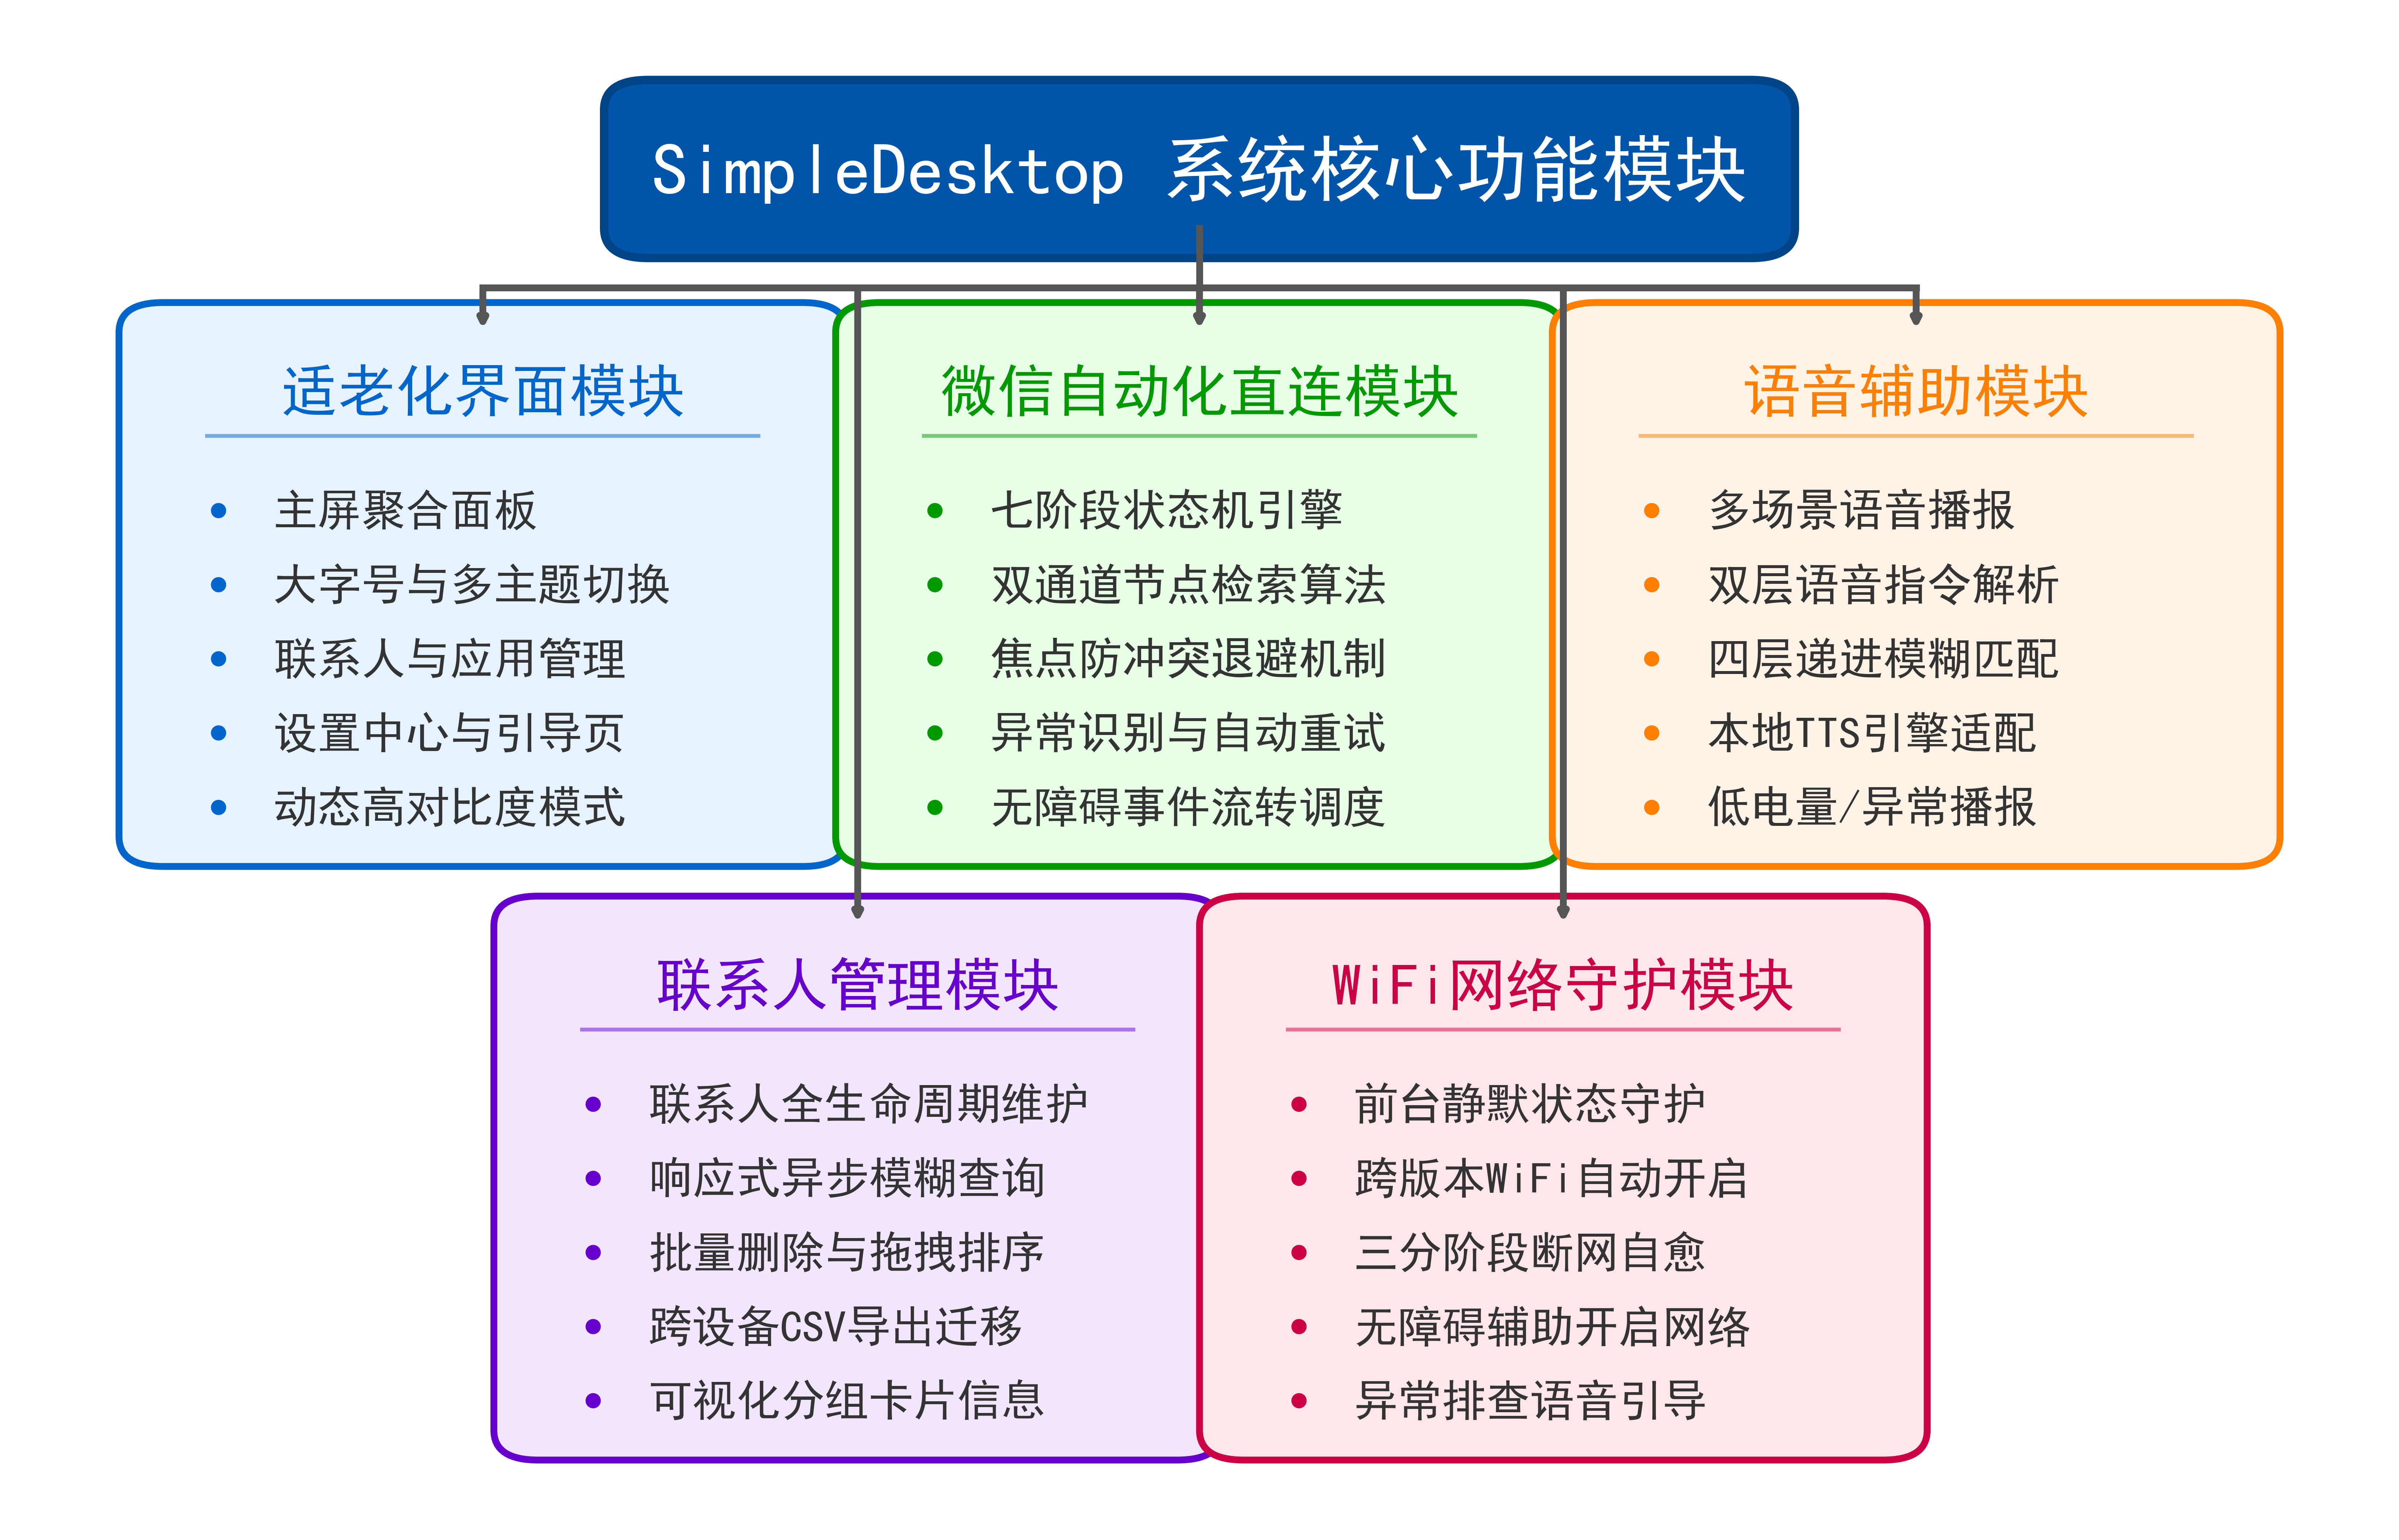
\includegraphics[width=\textwidth]{figures/fig3_1_system_modules.png}
    \caption{SimpleDesktop 适老桌面系统核心功能模块结构}
    \label{fig:system_modules}
\end{figure}


\subsection{开发环境}

本系统的开发与测试基于以下软硬件环境进行。开发主机选用搭载M系列处理器的MacBook Pro，操作系统为macOS 14.0。集成开发环境采用Android Studio Iguana（2023.2.1）正式版，构建工具为Gradle 8.6，编程语言为Kotlin 2.0.21，最低支持Android API 24（Android 7.0），目标API 34（Android 14），实际兼容性真机测试与适配覆盖了Android 14至Android 16的主流定制系统及HarmonyOS NEXT。版本控制采用Git结合Github代码托管平台。

系统所依赖的核心第三方库与版本如表3-1所示，涵盖了UI构建、依赖注入、数据持久化、网络请求、图片加载等关键能力。所有依赖均通过Gradle Version Catalog进行版本统一管理，确保依赖关系清晰可控。

\begin{table}[htbp]
  \centering
  \small
  \caption{主要开发依赖列表}
  \label{tab:development_dependencies}
  \renewcommand{\arraystretch}{1.3}
  \begin{threeparttable}
  \begin{tabular}{cll}
    \toprule
    \tableheader{序号} & \tableheader{模块层级} & \tableheader{依赖库与版本} \\
    \midrule
    \tablecell{1} & \tablecell{UI层} & \tablecell{Jetpack Compose 1.5.15、Material3、Compose Navigation\upcite{20,21}} \\
    \tablecell{2} & \tablecell{依赖注入} & \tablecell{Dagger-Hilt 2.56.2\upcite{24}} \\
    \tablecell{3} & \tablecell{数据持久化} & \tablecell{Room 2.6、DataStore Preferences\upcite{22,23}} \\
    \tablecell{4} & \tablecell{异步与响应式} & \tablecell{Kotlinx Coroutines\upcite{19}} \\
    \tablecell{5} & \tablecell{网络请求} & \tablecell{Retrofit 2 + OkHttp + Gson} \\
    \tablecell{6} & \tablecell{图片加载} & \tablecell{Coil} \\
    \tablecell{7} & \tablecell{权限管理} & \tablecell{XXPermissions} \\
    \tablecell{8} & \tablecell{农历计算} & \tablecell{Lunar Java库} \\
    \bottomrule
  \end{tabular}
  \end{threeparttable}
\end{table}


测试环境则覆盖多型号、多分辨率、多Android版本的真机环境，详细测试设备清单将在第4章测试章节中予以介绍。

\subsection{适老化界面模块}

（1）模块功能概述：
适老化界面模块负责构建符合老年用户视觉与认知特征的桌面交互界面，是用户与系统交互的第一接触面。模块主要包含主屏聚合面板、联系人管理界面、应用管理界面、设置中心、引导页、权限管理等子界面。

（2）主屏聚合面板设计：
主屏作为老年用户最频繁访问的界面，采用了卡片化的聚合面板设计。屏幕顶部为大尺寸时间天气信息卡，集中呈现实时时间（数字时钟，每秒刷新）、日期、星期、农历、天气图标、温度等高频信息。中部为两列卡片网格区，第一行预置手电筒卡片和语音助手卡片两个高频功能入口，第二行起依次平铺常用联系人卡片和常用应用卡片。整体布局遵循上信息、中操作、下扩展的视觉层次，老年用户无需滑动或跳转便可触达绝大多数日常操作入口。

（3）字号与主题动态切换：
考虑到不同老年用户对字号的偏好存在差异，系统提供小、中、大三档字号方案，每档对应一套完整的字号定义（涵盖标题、正文、说明文字等共15种字体角色）。当用户在设置中切换字号档位时，对应的字号配置通过响应式数据流向上传播，整个应用界面在下一帧自动按新字号重组刷新，无需重启应用。

主题模式上，系统提供经典蓝与暖心橙两套色彩方案。前者强调专业、冷静、稳重的视觉感受，后者突出温暖、亲切、活力的氛围，老年用户可根据个人喜好自由选择。此外系统还提供高对比度模式，将界面切换为黑底白字的高对比方案，特别适合视力较弱的老年用户。

（4）实现要点：
适老化界面模块基于Jetpack Compose声明式UI框架构建\upcite{20}。所有界面元素均通过可组合函数描述，状态由视图模型托管，主题、字号、对比度等全局参数通过Compose的CompositionLocal机制向下传递，确保整个组件树的一致性。列表类界面（如联系人列表、应用列表）采用LazyVerticalGrid组件实现惰性加载，仅渲染屏幕可见范围内的条目，保证大数据量下的滑动流畅性。

\subsection{微信自动化直连模块}
（1）模块功能概述：微信自动化直连模块是本系统的核心创新功能。其目标是将微信视频通话原本需要七步操作的流程，简化为老年用户在桌面上的一次点击。从用户视角看，老年用户只需点击桌面联系人卡片，在弹出的简洁面板中选择视频通话或语音通话，系统便自动完成微信内部所有后续操作并一步一步进入通话界面。

（2）业务流程难点分析：一键直拨方案的实现面临四方面难点。第一，目标应用界面不可控。微信作为第三方应用，其内部界面随版本迭代频繁变化，控件标识符可能因代码混淆或原生架构变动而失去稳定性\upcite{17}。第二，操作时序难以预测。微信内部页面切换的耗时受设备性能、网络状况等因素影响显著，过早或过晚的操作都可能导致流程失败。第三，外部干扰难以避免。在自动化流程执行过程中，可能突然出现来电通知、系统弹窗等外部干扰，导致焦点离开微信界面。第四，部分操作需要特殊处理。微信功能菜单中的通话选项不一定支持标准的点击事件触发，需要采用模拟手势的方式进行触发。

（3）七阶段状态机设计：针对上述难点，本模块将微信视频通话的自动化流程建模为一个七阶段的状态机\upcite{16}。状态机的设计借鉴了通信工程领域有限状态机模型的成熟思想，将复杂的动态过程分解为有限个相对独立、可观察、可验证、可重试的状态。


阶段一为微信主界面就位阶段。状态机检查当前活动窗口是否为微信主界面，若是则点击底部第一个标签页确保停留在聊天列表，若不是则通过系统返回操作逐步退回，直至到达主界面。

阶段二为搜索入口触发阶段。状态机定位主界面顶部的搜索图标并执行点击操作，使界面进入搜索页面。

阶段三为联系人姓名输入阶段。状态机定位搜索页面的输入框并将目标联系人的微信昵称写入，然后等待短暂的搜索响应时间。

阶段四为搜索结果确认阶段。状态机在搜索结果列表中点击与目标联系人匹配的条目，进入聊天界面。

阶段五为聊天功能展开阶段。状态机定位聊天界面右下方的功能菜单按钮并执行点击操作。

阶段六为通话选项选择阶段。状态机在展开的功能菜单中定位通话相关菜单项，并通过模拟手势方式在菜单项的中心坐标执行点击。

阶段七为通话类型确认阶段。如果上一阶段触发了通话类型选择弹窗，状态机进一步在弹窗中点击与用户偏好一致的通话方式选项，完成全部自动化流程后将状态机阶段索引重置为初始值。

\begin{figure}[!ht]
  \centering
  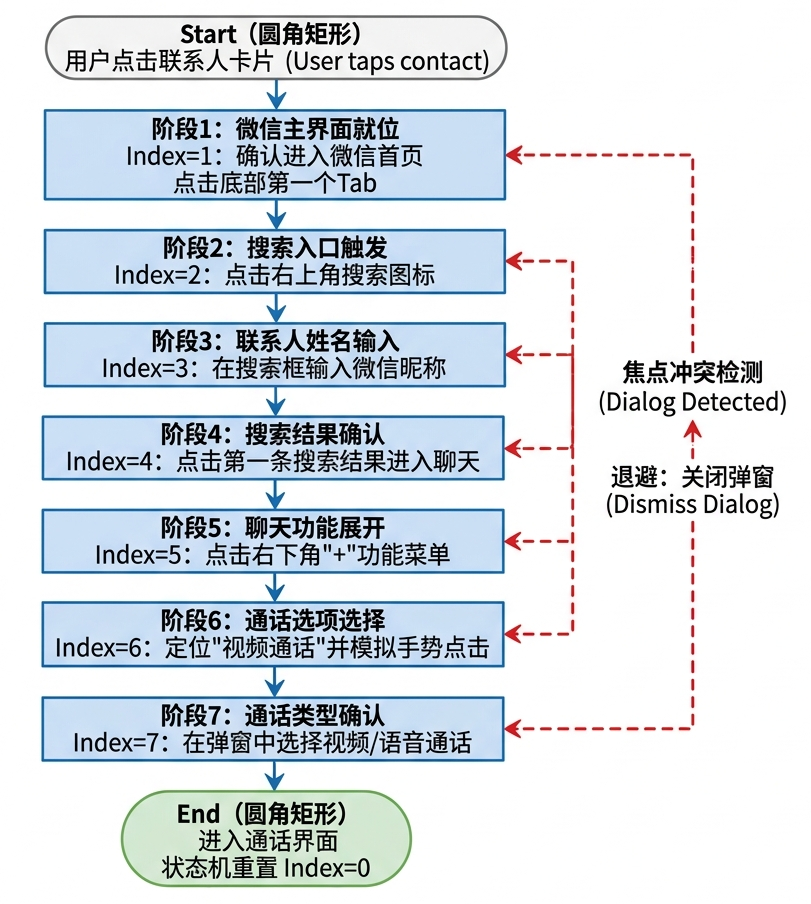
\includegraphics[width=0.6\textwidth]{figures/wechat_state.png}
  \caption{微信一键直拨七阶段状态机流程}
  \label{fig:wechat_state_machine}
\end{figure}

七个阶段之间通过事件驱动加状态推进的方式协作。每个阶段在自身操作完成后等待数百毫秒至一秒不等的时间，使界面切换得以完成，然后将状态机阶段索引推进至下一阶段。下一次窗口状态变化或内容变化事件被触发时，状态机便在新的界面上继续执行下一阶段。



（4）双通道节点检索算法：为应对微信版本更新带来的控件标识符变化问题，本模块设计了双通道节点检索算法\upcite{17}。算法的核心思想是同时利用控件标识符和文本内容两类不同性质的信息进行节点定位，在主通道失效时自动切换到备用通道。

在每次需要定位界面节点时，算法首先尝试通过控件标识符查找节点。这一通道使用控件树的标识符索引，时间复杂度极低，在标识符稳定时能够快速准确地命中目标。如果通过控件标识符未能找到目标节点，算法立即切换到第二通道，通过文本内容进行查找。第二通道遍历控件树查找匹配文本的节点，虽然时间复杂度相对较高，但具备良好的稳定性。

双通道协同的设计将高效与稳健有机结合：在通常情况下系统享受第一通道带来的高效执行，在异常情况下又能依靠第二通道避免完全失败。实测在微信8.0.30到最新版本的多个版本上，整体流程成功率均保持在99.1\%以上，平均流程耗时为5至6秒。

（5）焦点防冲突退避机制：焦点冲突是指自动化流程预期操作的目标窗口与实际处于活动状态的窗口不一致的情况。当焦点冲突发生时，无障碍服务读取到的活动窗口节点树将不再属于微信主界面，而属于干扰窗口，可能导致流程失败甚至产生意外行为\upcite{13}。

针对焦点冲突，本模块设计了识别异常、主动退避、等待恢复、自动重试的退避策略。无障碍服务在每次接收到事件时，检查当前活动窗口的类名是否包含典型的对话框关键字。一旦检测到对话框存在，便立即通过系统返回操作主动关闭对话框。退避操作完成后，状态机不推进到下一阶段，而是保持在当前阶段等待下一次窗口事件触发。整个退避、恢复、重试过程对老年用户完全透明，用户只会感觉到流程稍有延迟但最终成功完成。

\subsection{WiFi网络守护模块}

WiFi是老年用户语音通话、视频连线的核心通信保障，其稳定性直接影响系统可用性。

（1）模块功能概述：WiFi网络守护模块旨在解决老年用户因误触WiFi开关或路由器信号波动导致的网络异常问题，确保终端通信链路的连续性。模块由前台守护服务、网络回调监听、WiFi自动开启无障碍服务、用户引导面板四部分组成，形成完整的检测、等待、自愈、引导闭环。

（2）前台守护服务：为实现网络状态的持续监测，模块采用前台服务模式运行后台守护逻辑。前台服务通过在系统通知栏显示一条低优先级、静默模式的常驻通知向操作系统表明服务的活跃性，从而获得较高的进程保活优先级。服务启动后立即向系统的连接管理器注册WiFi类型的网络回调监听，实时感知WiFi连接状态变化。

（3）基于无障碍服务的WiFi自动开启：由于系统安全性与隐私保护设计，自 Android 10及以上版本起（本系统实际测试覆盖的Android 14至16均适用），操作系统不再允许应用通过编程接口直接控制WiFi开关。因此，本模块统一采用无障碍服务辅助开启的方案：当检测到网络异常需要开启WiFi时，模块设置无障碍服务的工作标志位，并主动跳转到系统WiFi设置页面；专门设计的WiFi自动开启无障碍服务监听设置页面的事件，自动定位并点击WiFi开关，操作完成后通过模拟Home键返回桌面。整个过程对老年用户完全透明\upcite{13}。整个守护与自愈的详细流程机制如下图所示：

\begin{figure}[h]
  \centering
  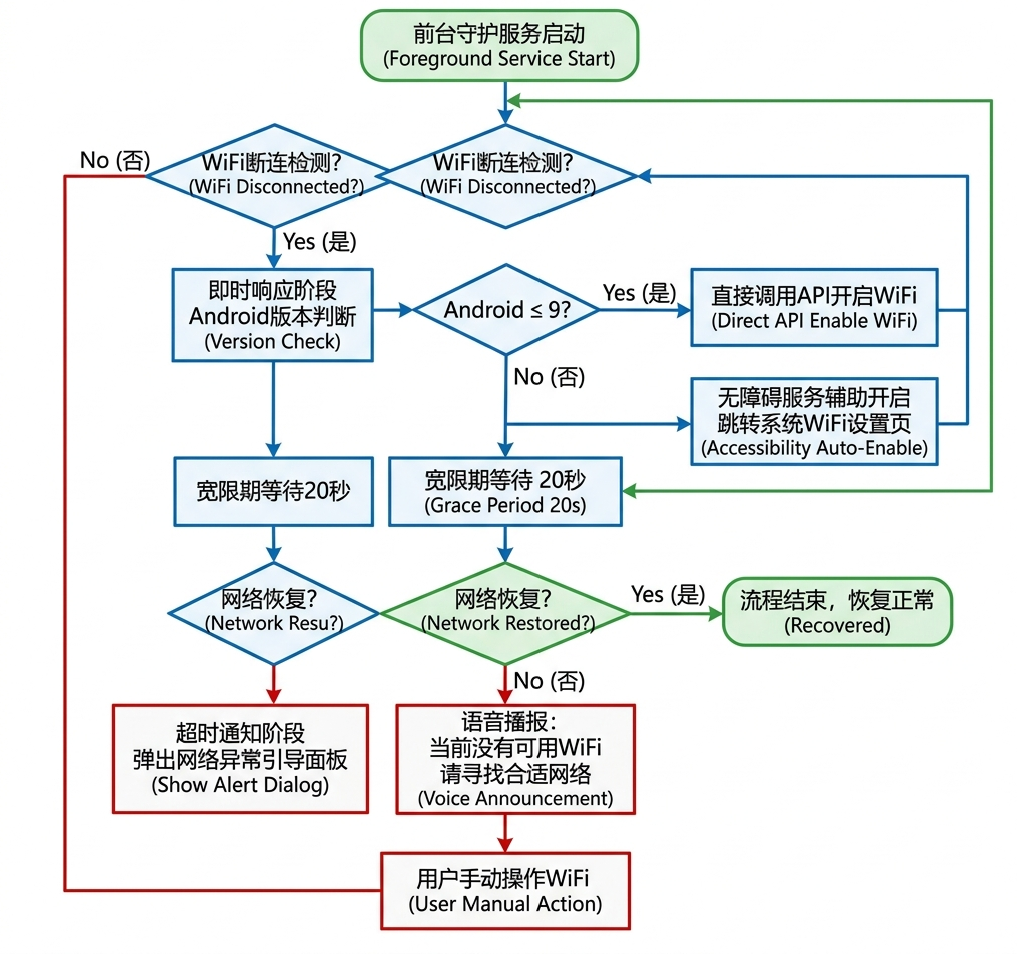
\includegraphics[width=1.0\textwidth]{figures/wifi_daemon.png}
  \caption{WiFi网络守护与自愈机制流程}
  \label{fig:wifi_daemon}
\end{figure}

（4）断网自愈与引导面板：断网自愈策略由即时响应、宽限等待、超时通知三个阶段构成。即时响应阶段在断连事件发生瞬间立即调用WiFi自动开启逻辑；宽限等待阶段给系统留出充分的恢复时间，期间持续监测网络状态，一旦连接恢复立即结束自愈流程；超时通知阶段在宽限期结束仍未恢复时，通过广播触发界面层的网络异常提示弹窗，并由语音助手播报“无可用网络”的语音提示，引导老年用户进行下一步操作。

网络异常提示弹窗采用大尺寸卡片式布局设计，主标题以醒目的字号和颜色呈现无可用WiFi网络，副标题以适中字号补充说明请寻找合适的网络连接，底部提供清晰的操作按钮。点击打开WiFi设置按钮后，系统直接跳转到Android的WiFi设置面板，老年用户完成WiFi连接后可直接返回桌面。

\subsection{语音辅助模块}

（1）模块功能概述：语音辅助模块由语音播报与语音指令解析两个子模块组成，旨在为视力不佳或不擅长触屏操作的老年用户提供听觉通道与语音通道的辅助交互。

\begin{figure}[htbp]
  \centering
  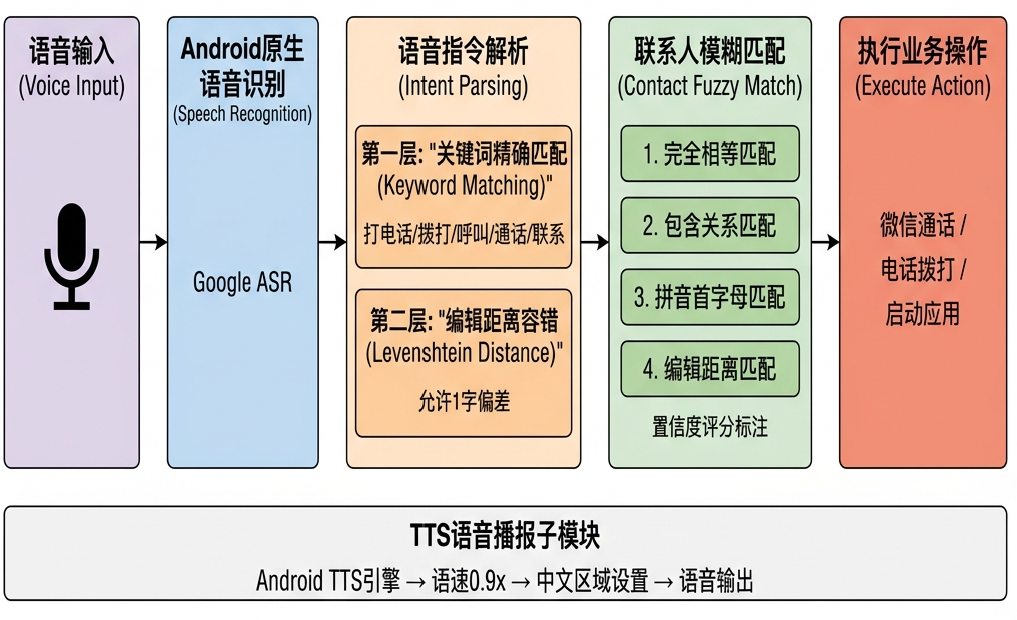
\includegraphics[width=1.0\textwidth]{figures/voice_flow.png}
  \caption{语音辅助模块工作流程}
  \label{fig:voice_assistant_flow}
\end{figure}


（2）语音播报子模块：语音播报基于Android原生的文本转语音引擎封装实现，提供统一的语音播报接口，覆盖网络异常提示、操作执行确认、低电量提醒等多个使用场景。模块在初始化时尝试多种中文区域设置，以兼容不同手机厂商TTS引擎对中文支持的差异；语速默认设置为正常速度的0.9倍，使语音节奏更适合老年人的听觉接受能力。


（3）语音指令解析子模块：语音指令解析采用关键词匹配加编辑距离容错的轻量级双层策略\upcite{18}。第一层为关键词精确匹配，模块为每种支持的动作类型（包括打电话、打开应用、开关手电筒等）维护一组对应的关键词库（如打电话动作的关键词包括打电话、拨打、呼叫、通话、联系等十余个），通过遍历检查输入文本中是否包含某个关键词来识别用户意图。

第二层为编辑距离容错匹配，主要应对老年人发音不标准或语音识别引擎识别误差的情况。算法对输入文本中与关键词等长的每个子串计算与该关键词的编辑距离，允许一个字符的偏差即视为匹配。这种容错机制使系统在面对识别误差时依然能够正确理解用户意图。

（4）联系人模糊匹配：在识别出打电话动作意图后，系统还需要将用户说出的联系人名称与通讯录中的实际联系对象进行匹配。模块采用四层递进的联系人模糊匹配策略：完全相等匹配、包含关系匹配、拼音首字母匹配和编辑距离匹配\upcite{18}，每一层匹配赋予不同的置信度评分。系统从最严格的完全相等匹配开始尝试，逐层放宽至最宽松的编辑距离匹配，并最终选择置信度最高且超过预设阈值的匹配结果作为目标联系人。



\subsection{联系人管理模块}
（1）模块功能概述：联系人管理模块为老年用户提供常用联系对象的全生命周期管理能力，覆盖联系人的新增、查询、修改、删除、排序、导出等核心功能，是支撑通讯类业务的基础数据模块。

（2）联系人新增与编辑：联系人新增界面采用分组卡片式布局，依次包含基本信息组（姓名、电话号码、微信昵称）、头像组（支持从相册选择或现场拍照）和通话能力组（视频通话、语音通话、电话直拨三个开关）。所有输入控件均采用大字号、宽边距设计，方便老年用户的视觉辨识与触摸操作。

联系人编辑界面与新增界面布局一致，区别在于初始数据由数据库回填，用户可直接修改现有信息。保存操作通过响应式数据流自动同步到数据库与主屏。

（3）联系人查询：联系人查询支持按姓名进行模糊搜索。用户在搜索框中输入任意关键字后，系统在协程中异步执行数据库的LIKE查询，并将结果通过Flow实时推送到界面层\upcite{19}。配合Compose的状态收集机制，搜索结果在用户输入的同时即时呈现，无需点击搜索按钮。

（4）联系人删除与排序：联系人删除支持单条删除与批量删除两种模式。为防止老年用户误操作，删除前系统弹出确认对话框，明确告知删除将不可撤销。

联系人排序由分配排序索引字段实现。用户可通过拖拽方式手动调整联系人在主屏上的显示顺序，新顺序通过协程异步写入数据库后立即反映到界面。

（5）联系人导出：为方便老年用户在更换设备时迁移联系人数据，系统提供联系人导出功能。导出格式为标准CSV文本文件，包含全部联系人字段，文件保存在设备的下载目录，可通过微信、邮件等渠道分享给子女进行备份。

\section{软件操作流程}

\subsection{首次启动与初始化流程}
用户首次安装并启动SimpleDesktop后，系统进入引导页流程。引导页通过左右滑动的方式依次介绍系统的核心功能特点（适老化界面、一键通话、网络守护、语音助手），帮助老年用户或其家属快速建立对系统能力的整体认知。


\begin{figure}[H]
    \centering
    \begin{minipage}{0.22\textwidth}
        \centering
        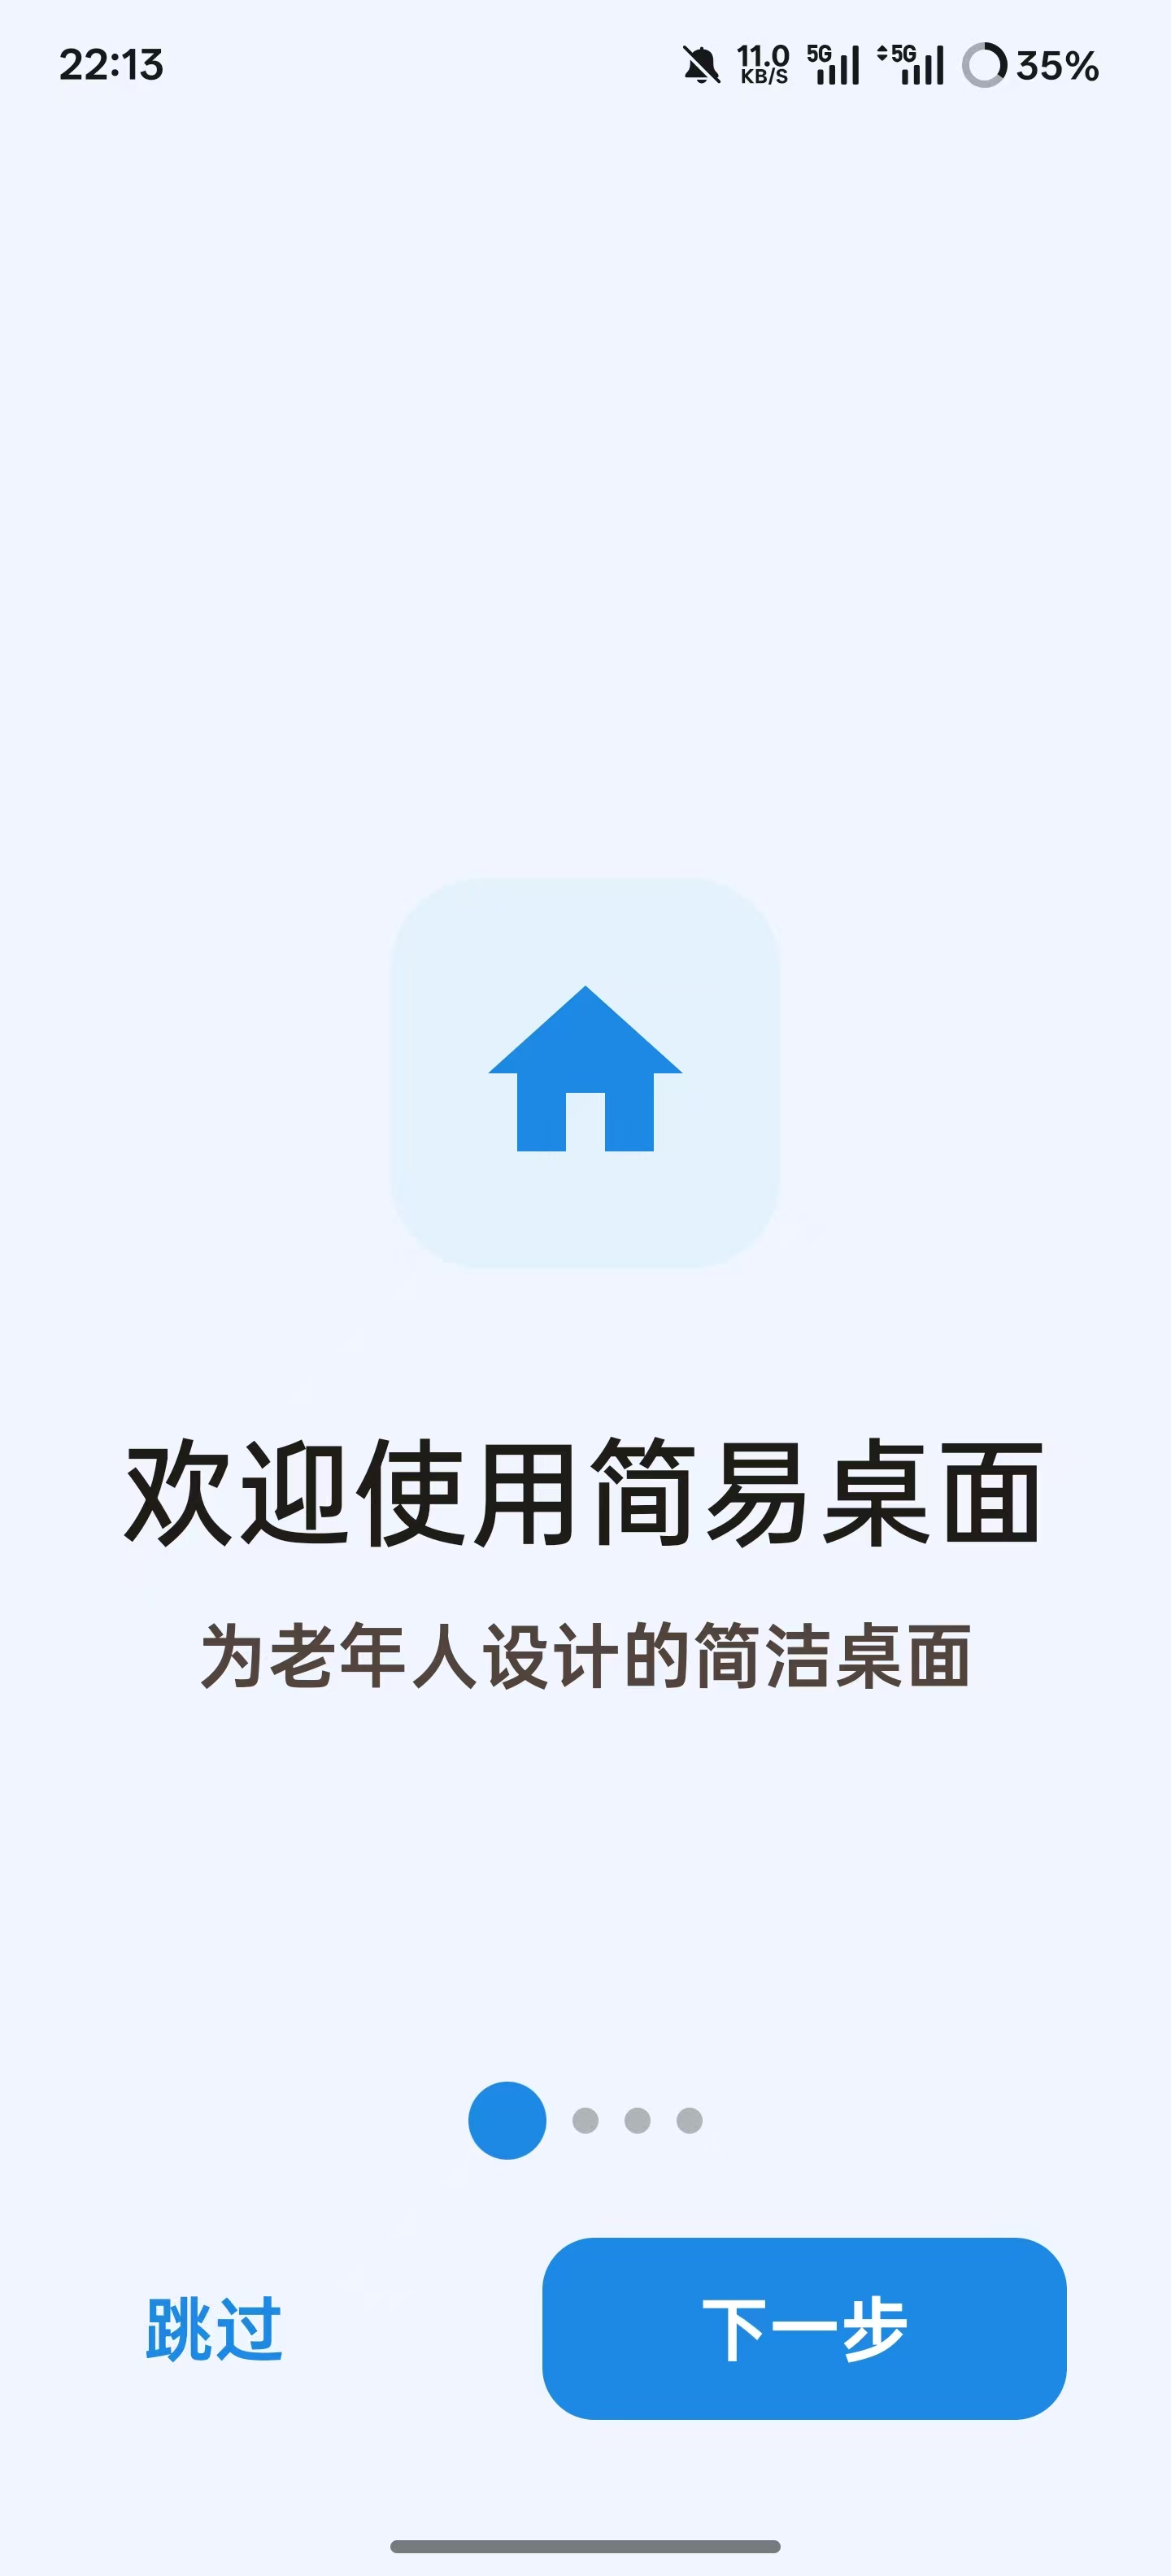
\includegraphics[width=\linewidth]{figures/wechat/desktop1.jpg}
        \caption*{(a) 首次启动}
    \end{minipage}\hfill
    \begin{minipage}{0.22\textwidth}
        \centering
        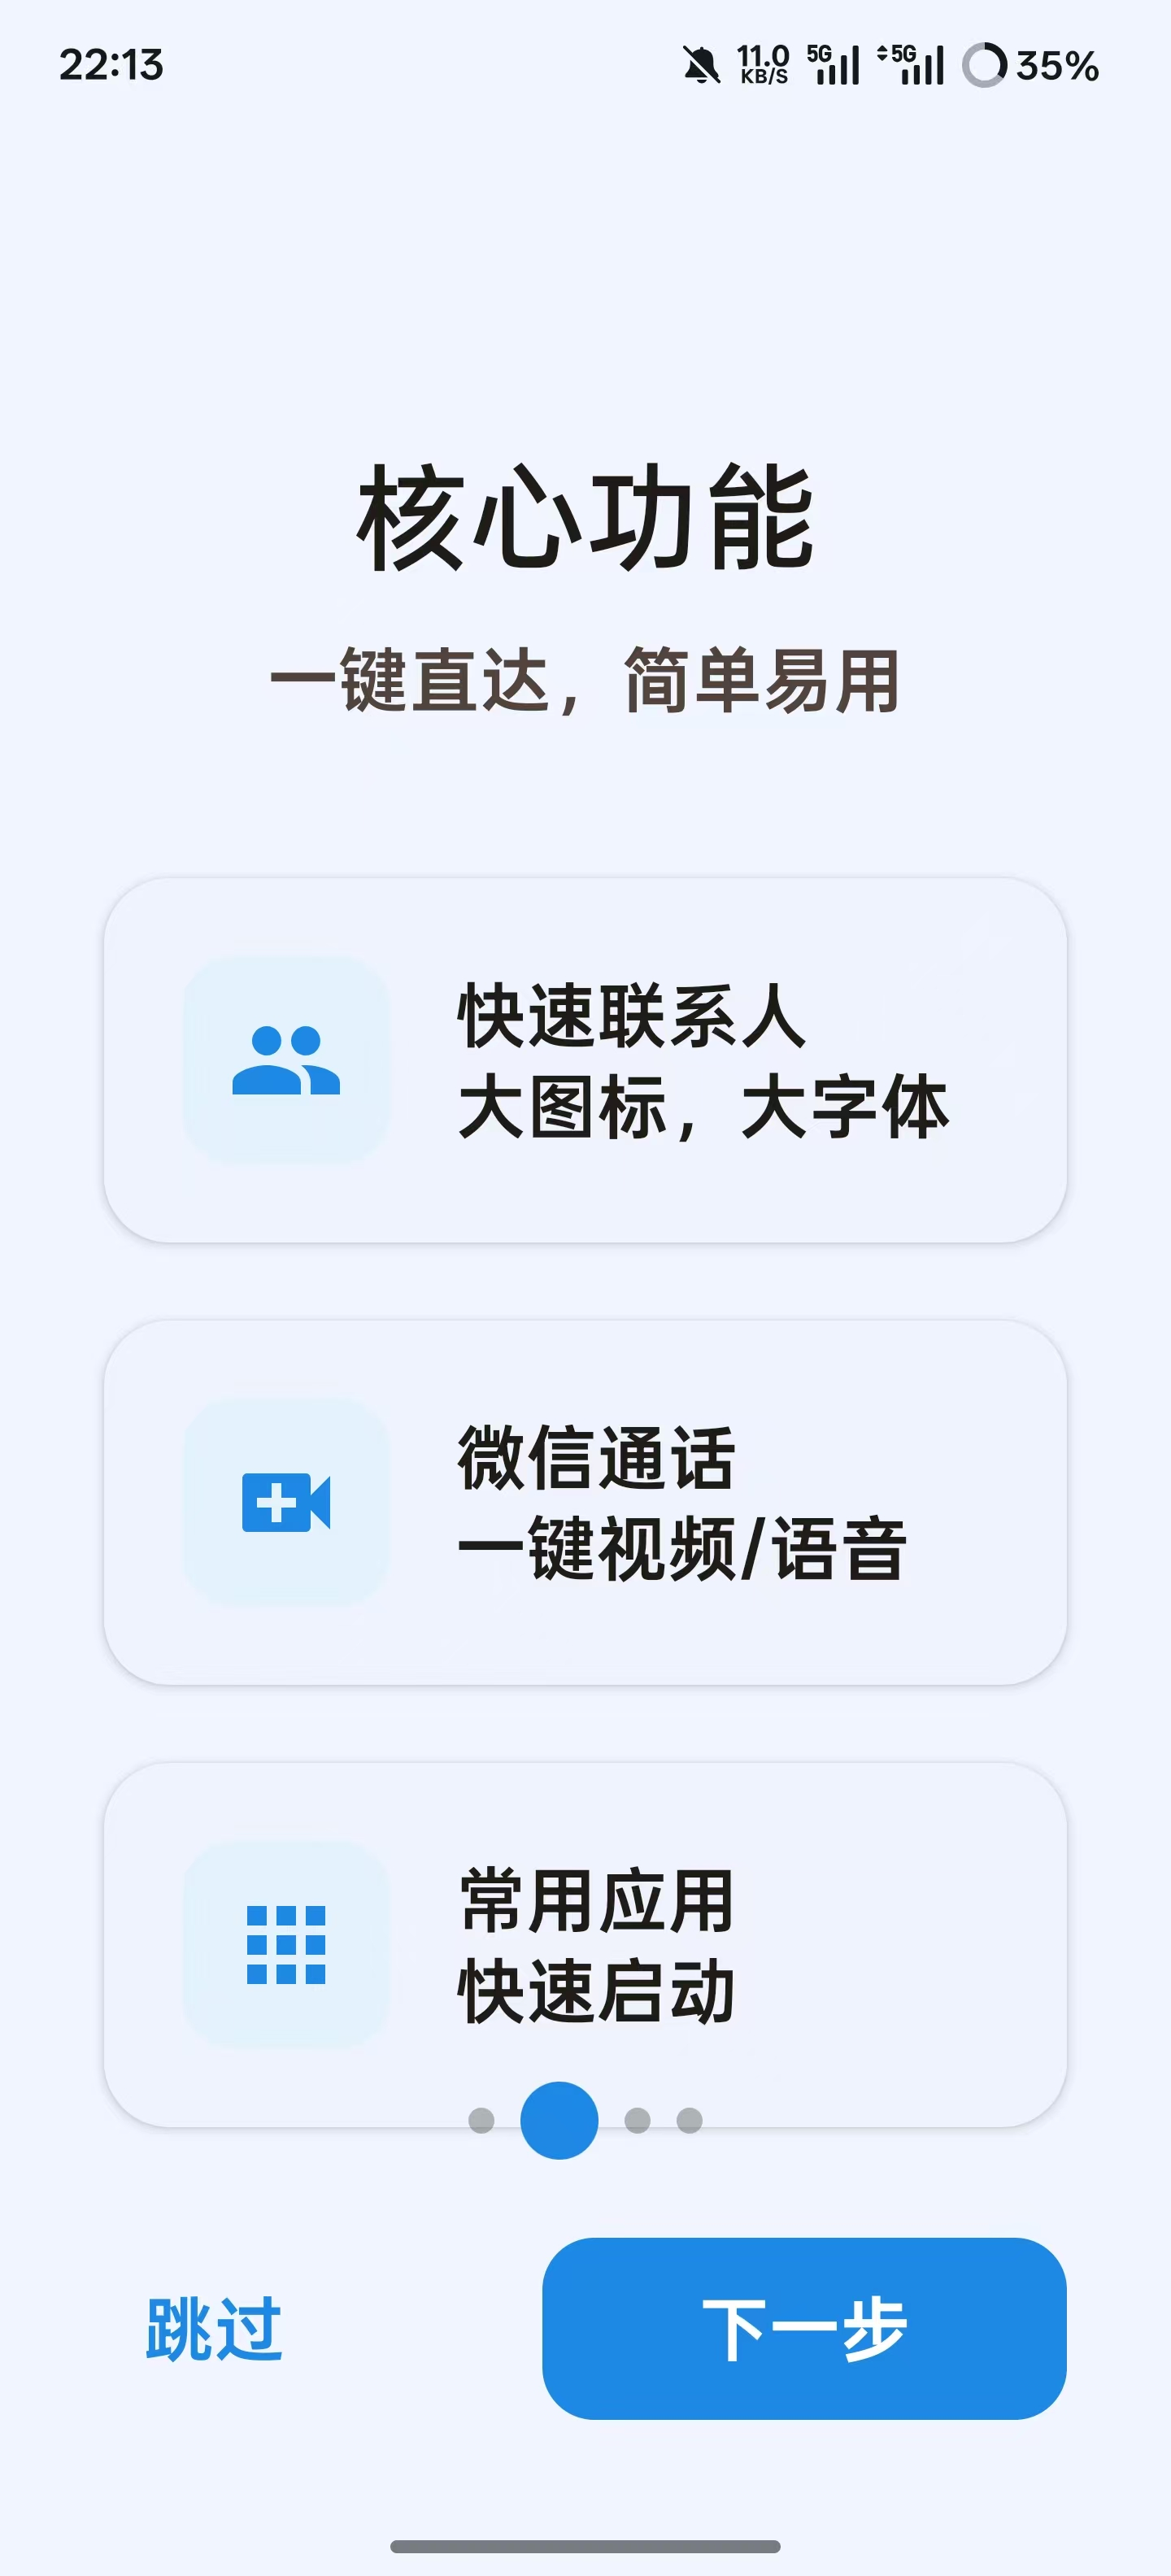
\includegraphics[width=\linewidth]{figures/wechat/desktop2.jpg}
        \caption*{(b) 功能介绍}
    \end{minipage}\hfill
    \begin{minipage}{0.22\textwidth}
        \centering
        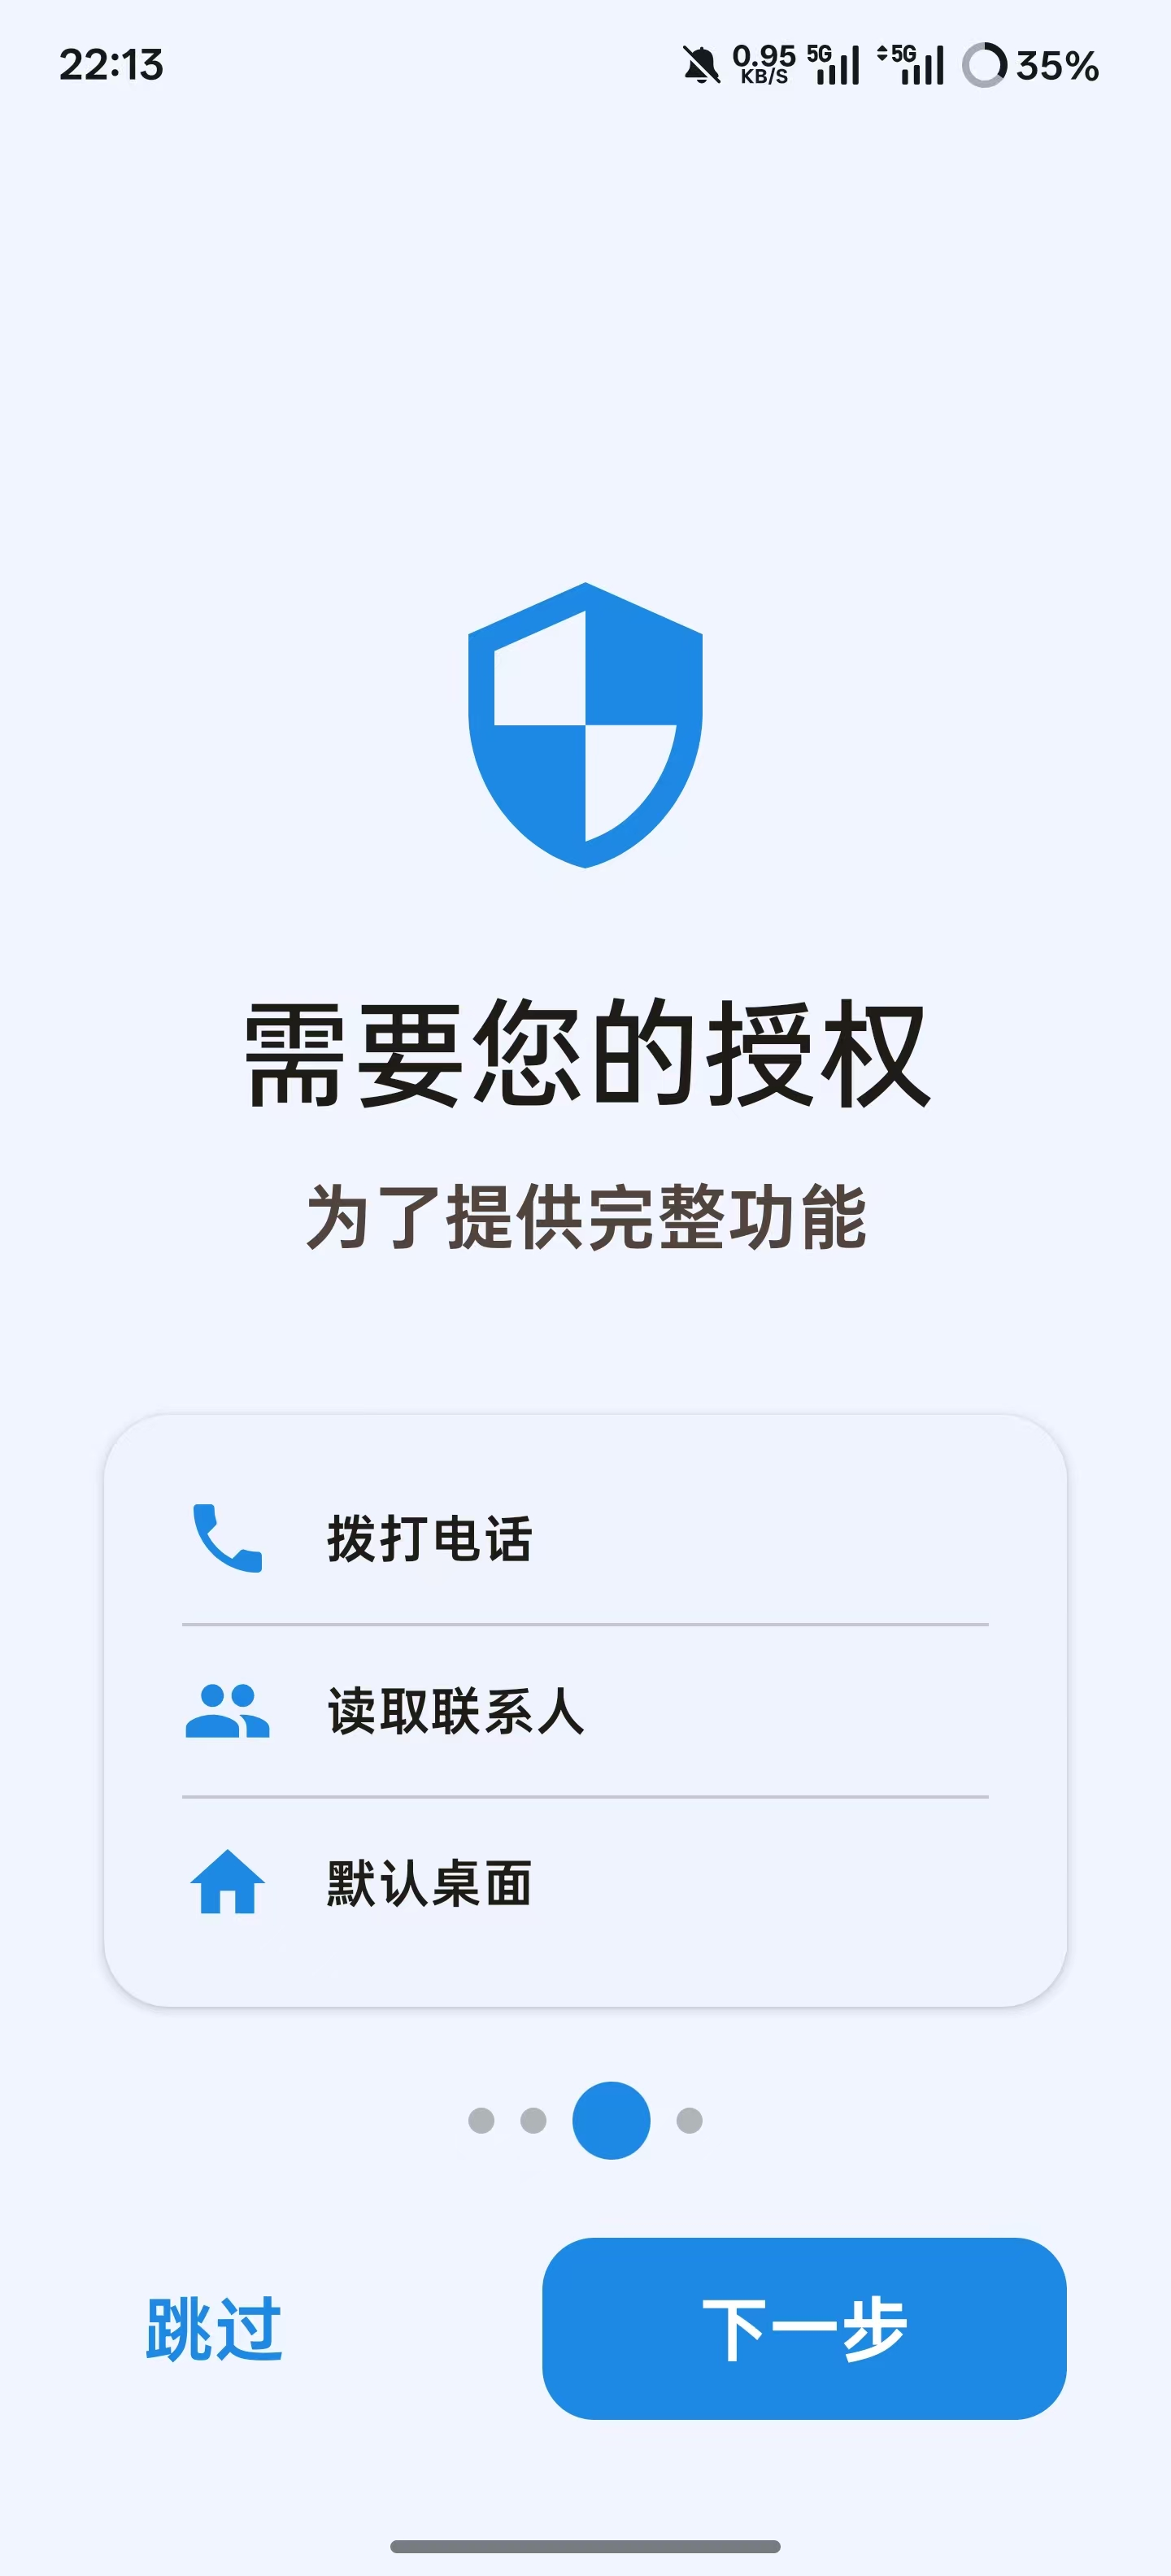
\includegraphics[width=\linewidth]{figures/wechat/desktop3.jpg}
        \caption*{(c) 权限授权}
    \end{minipage}

    \vspace{0.3cm}

    \begin{minipage}{0.22\textwidth}
        \centering
        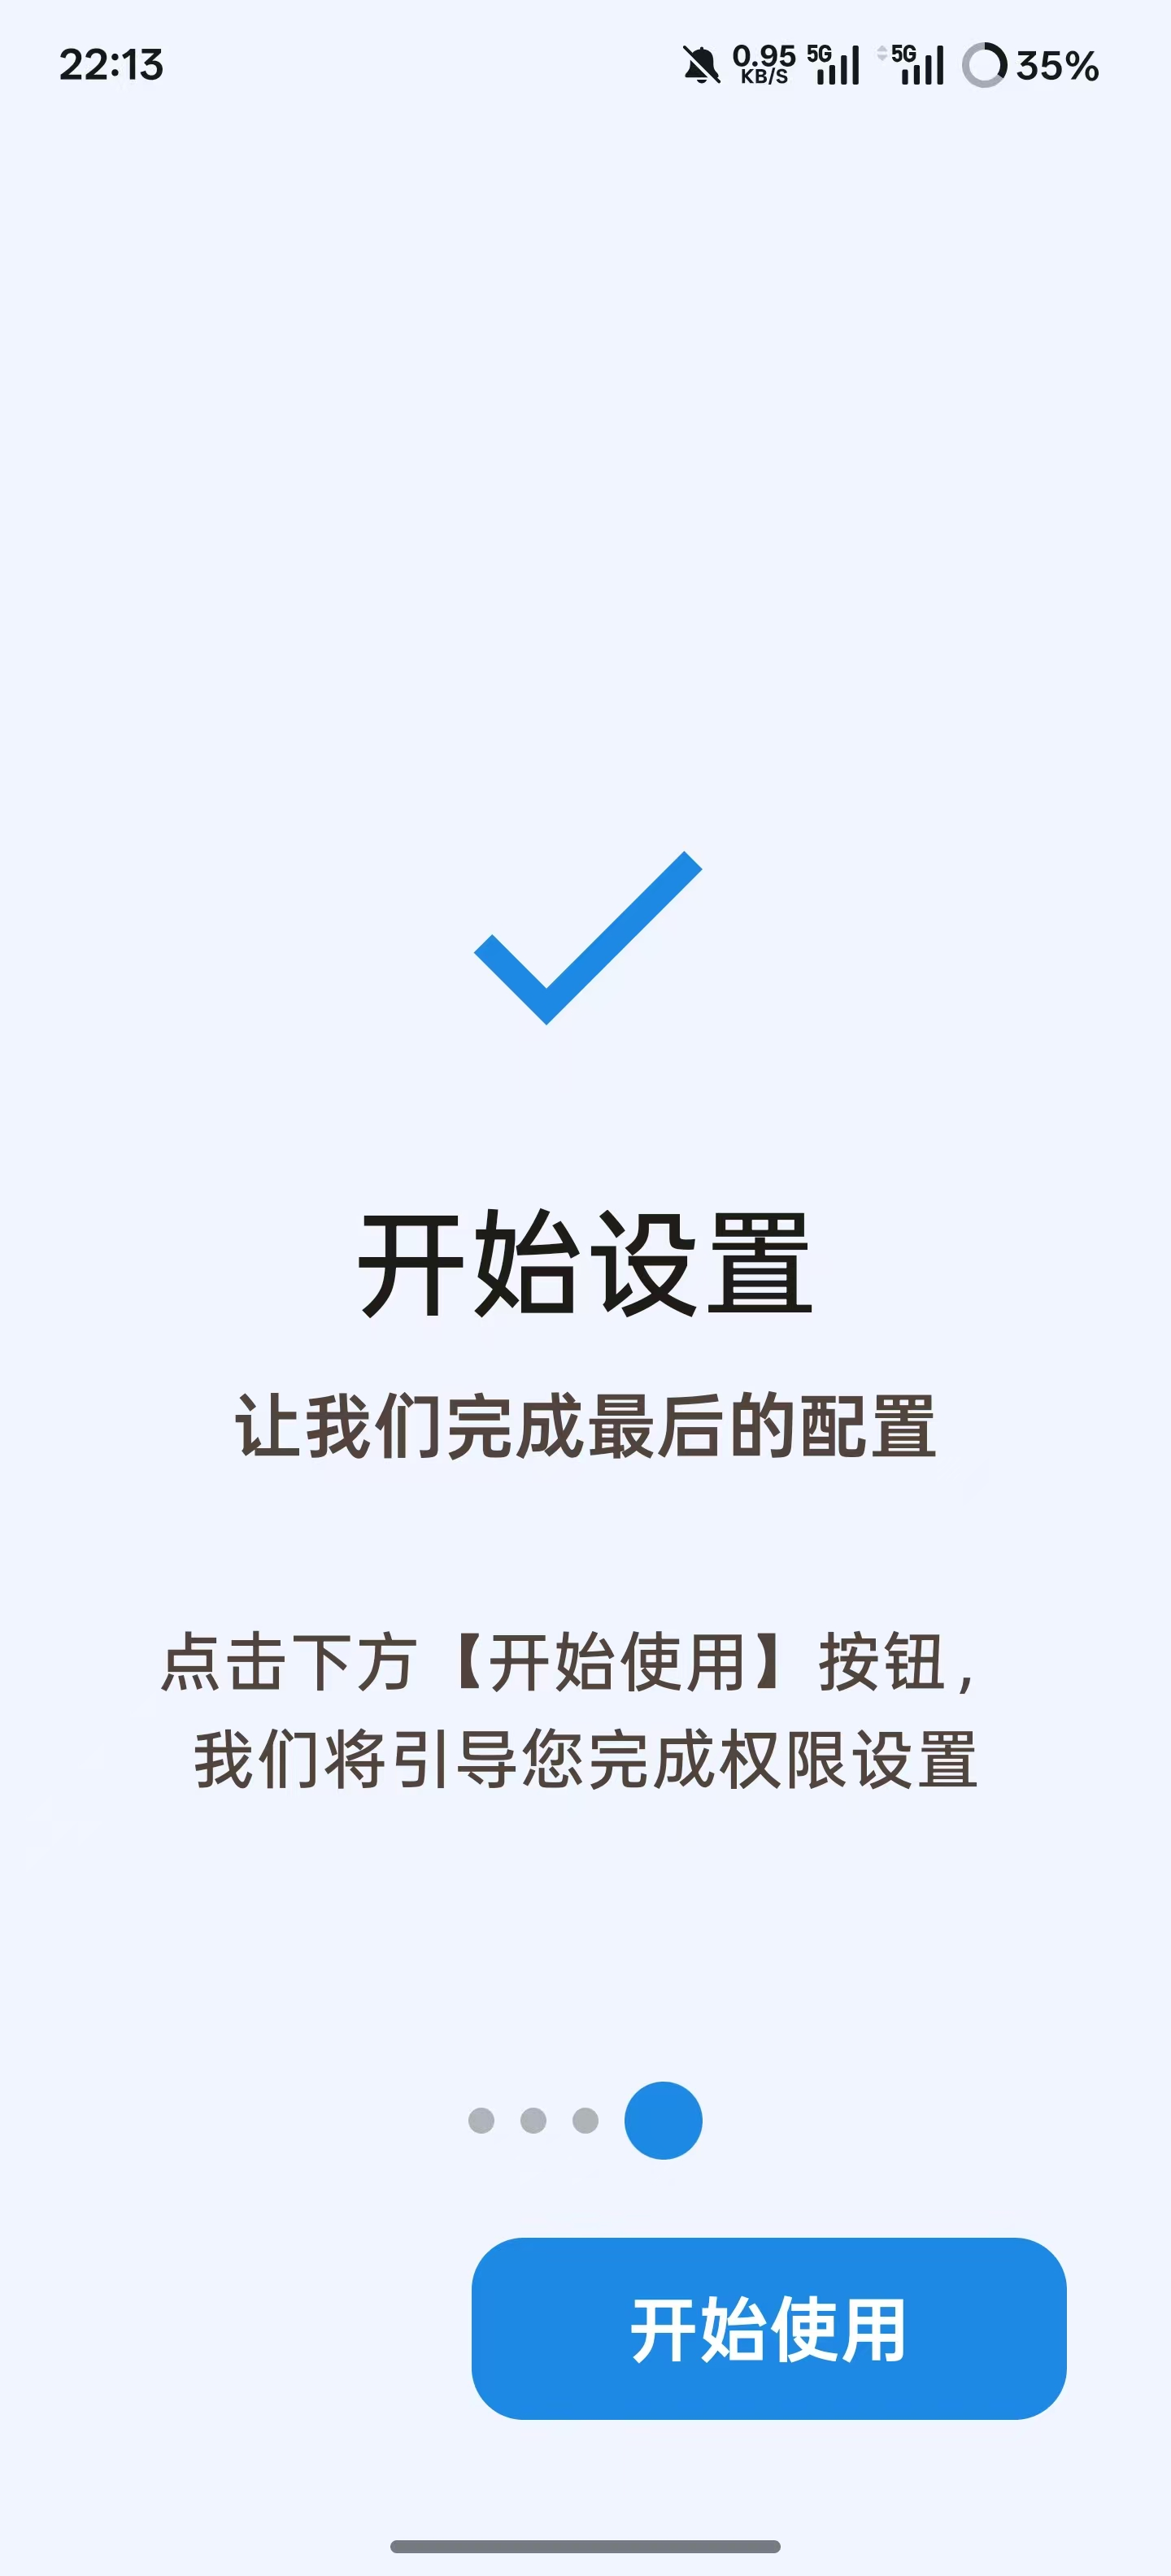
\includegraphics[width=\linewidth]{figures/wechat/desktop4.jpg}
        \caption*{(d) 开始设置}
    \end{minipage}\hfill
    \begin{minipage}{0.22\textwidth}
        \centering
        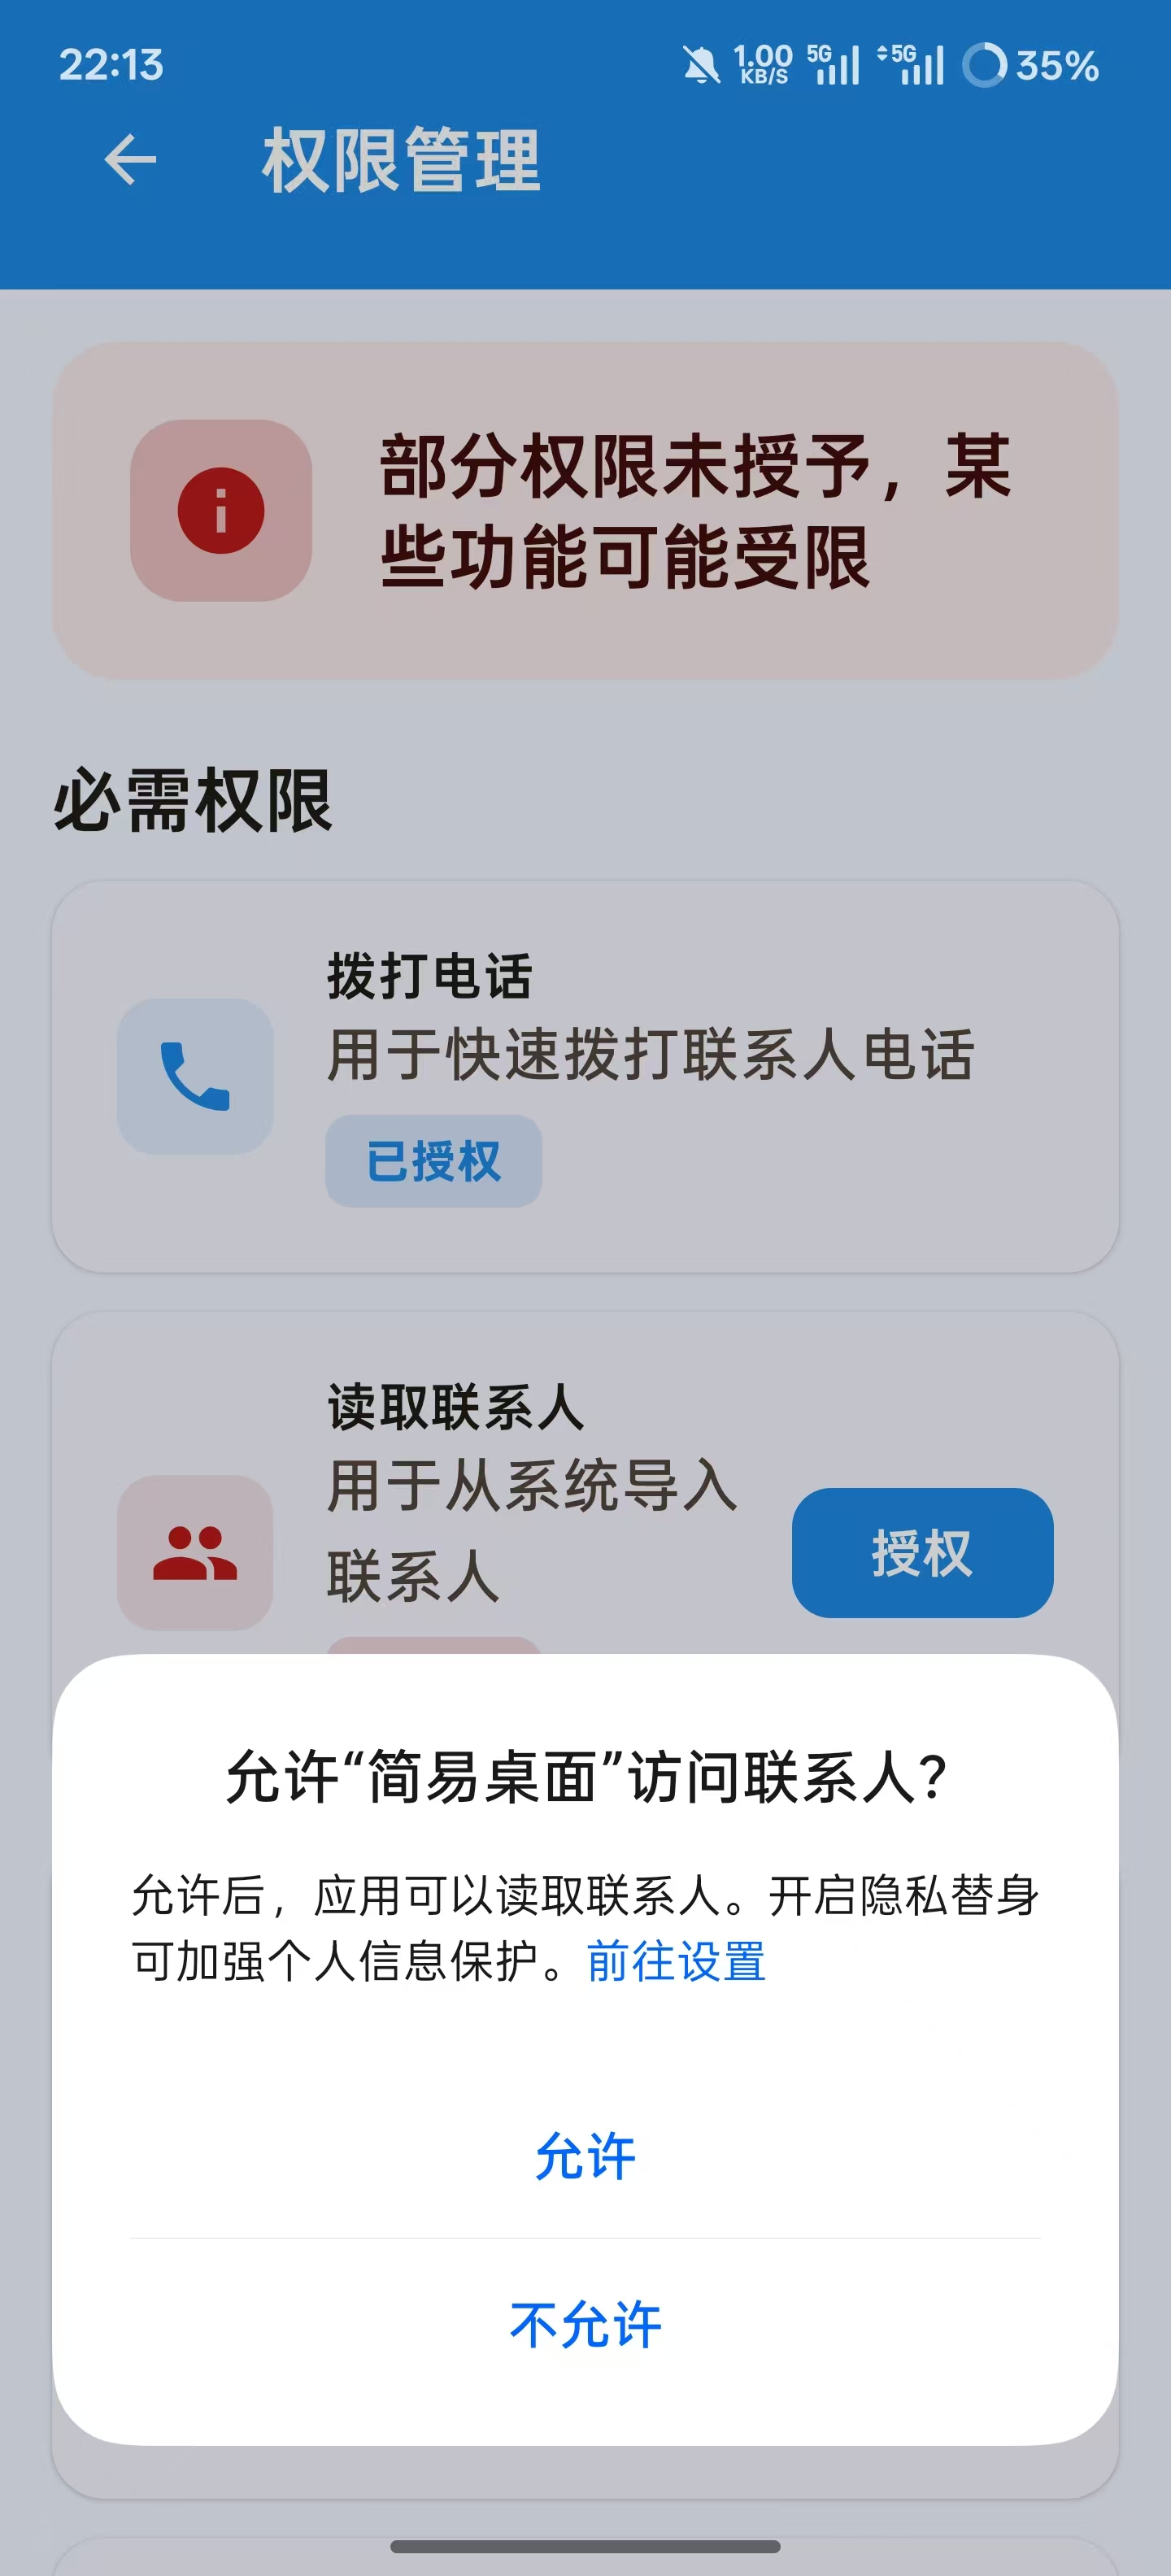
\includegraphics[width=\linewidth]{figures/wechat/desktop5.jpg}
        \caption*{(e) 权限设置}
    \end{minipage}\hfill
    \begin{minipage}{0.22\textwidth}
        \centering
        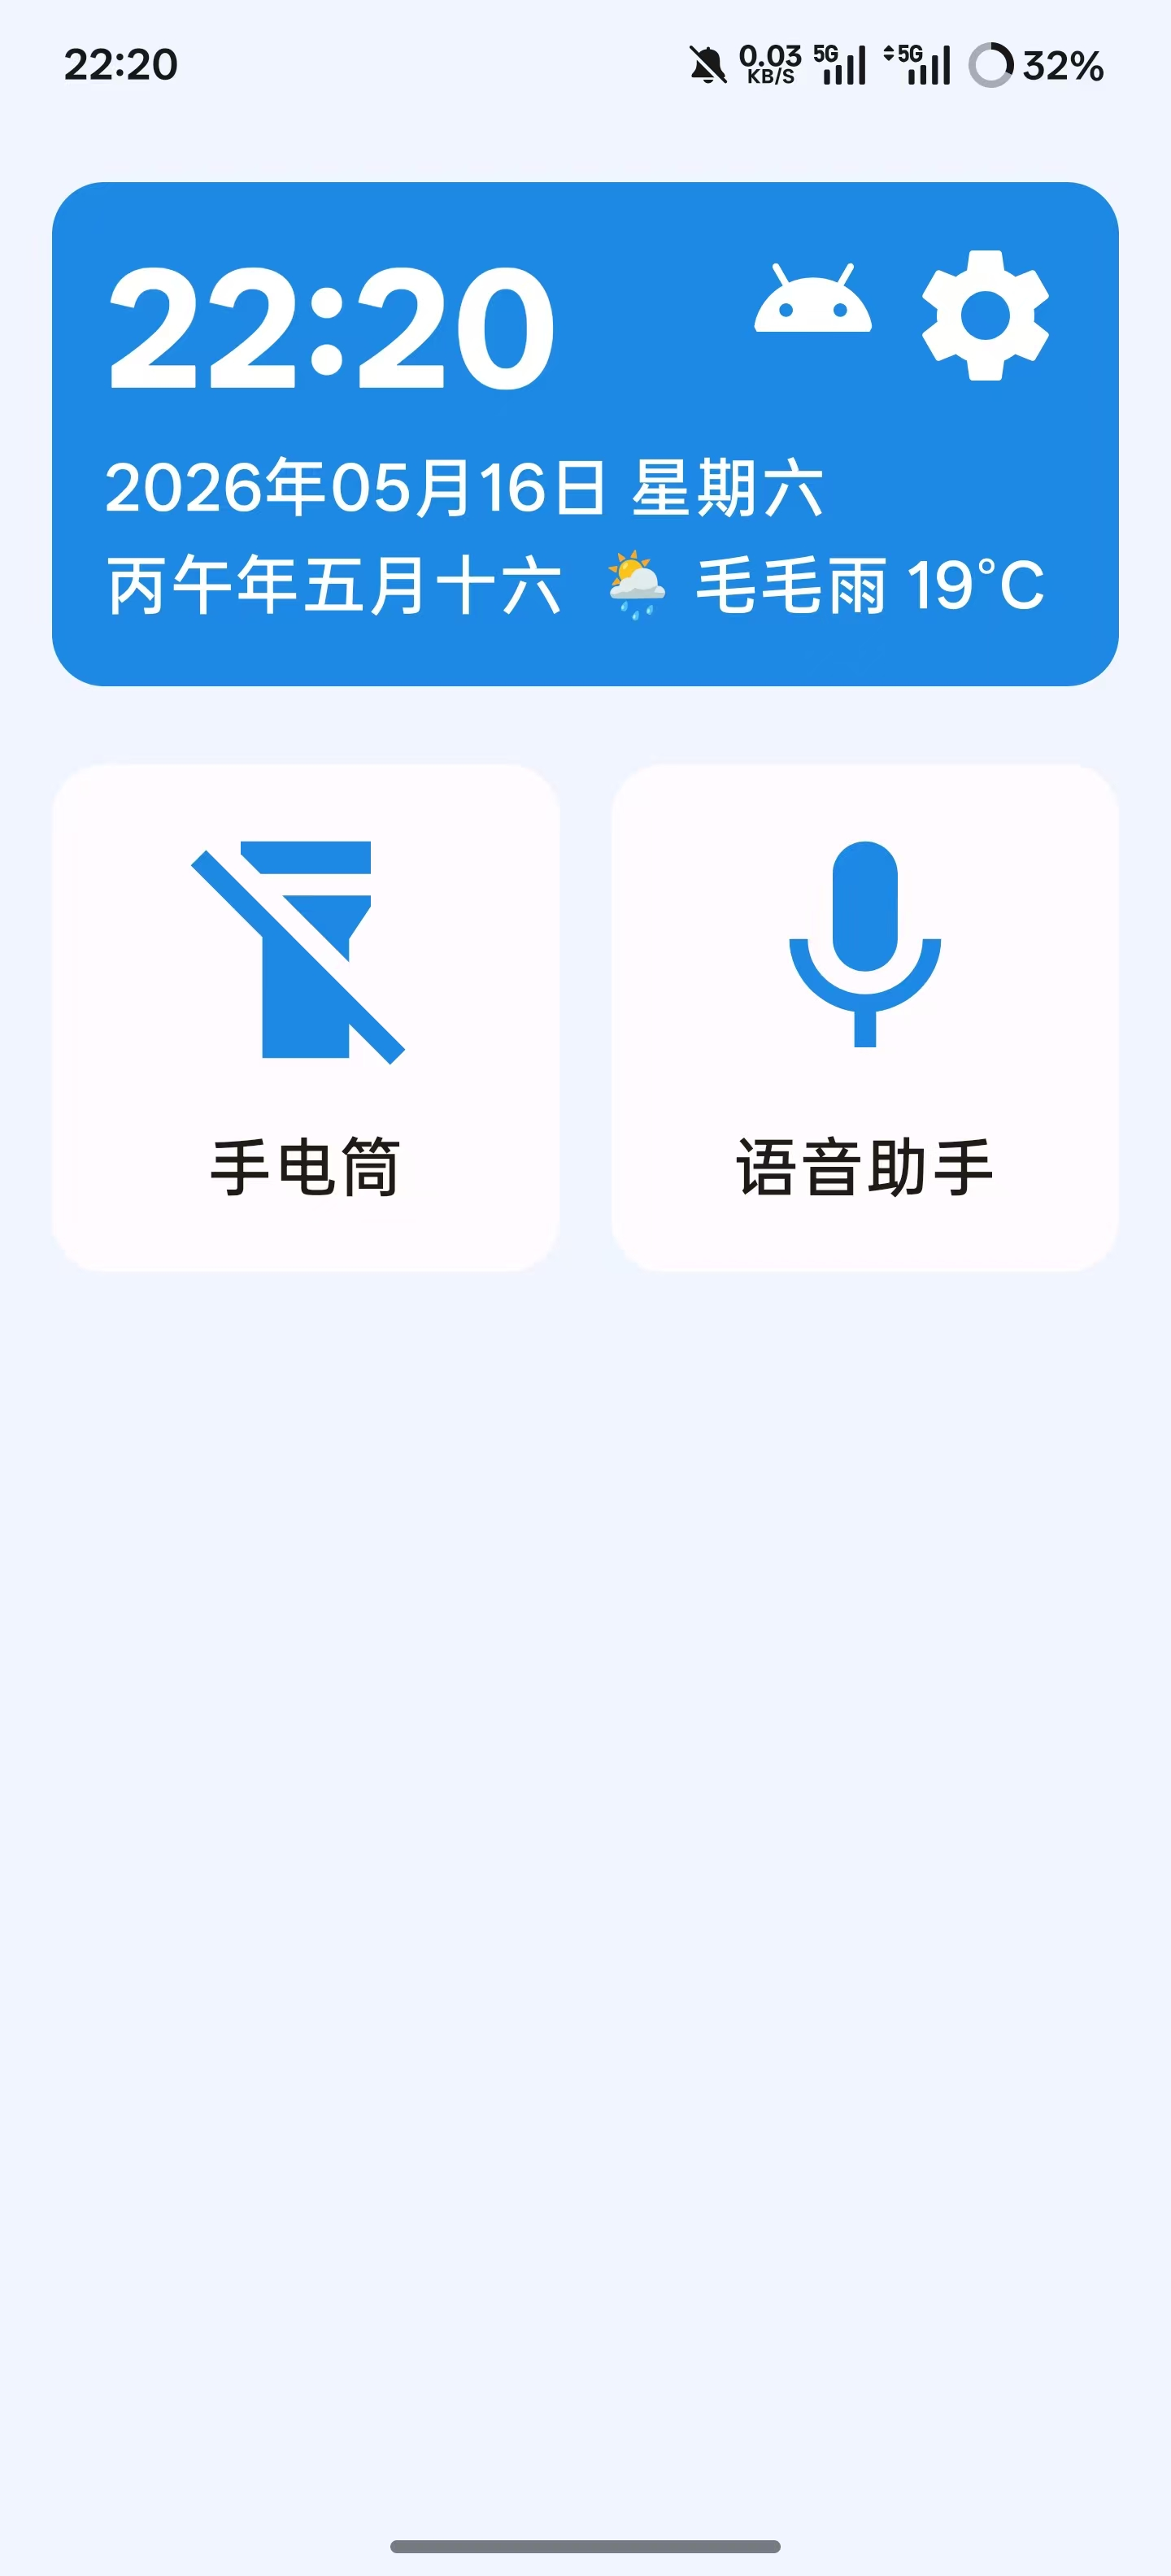
\includegraphics[width=\linewidth]{figures/wechat/desktop6.jpg}
        \caption*{(f) 初始主页}
    \end{minipage}
    \caption{SimpleDesktop 简易桌面首次启动页面}
    \label{fig:wechat_first_boot}
\end{figure}


滑动至最后一页时，引导页提供完成引导按钮，点击后系统自动跳转至权限申请页面，依次申请电话拨打权限、读取联系人权限、相机权限（用于拍摄头像）、位置权限（用于天气定位）等运行时权限。如果当前设备运行在Android 6.0及以上版本且尚未授权，系统会通过XXPermissions权限框架弹出系统级权限对话框；老年用户可在子女协助下完成授权操作。

权限授权完成后，系统提示用户开启无障碍服务\upcite{13}，这是微信一键直拨与WiFi自动开启功能的前置条件。系统通过专门设计的引导对话框图文并茂地说明授权步骤，并提供一键跳转到无障碍设置页的快捷入口。完成无障碍授权后，系统将自身设置为默认桌面应用，此时初始化流程结束，用户进入主屏。



\subsection{日常使用主流程}

在日常使用中，老年用户启动设备后直接进入SimpleDesktop主屏。主屏顶部实时显示当前时间、日期、农历和天气，让老年用户对当下信息一目了然。

\begin{figure}[htbp]
    \centering
    \begin{minipage}{0.22\textwidth}
        \centering
        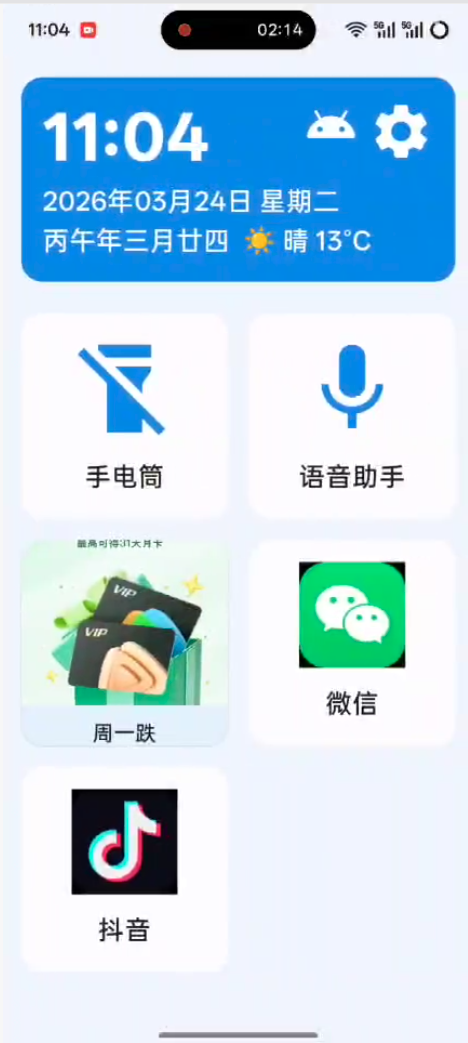
\includegraphics[width=\linewidth]{figures/demo1.png}
        \caption*{(a) 桌面触发状态}
    \end{minipage}\hfill
    \begin{minipage}{0.22\textwidth}
        \centering
        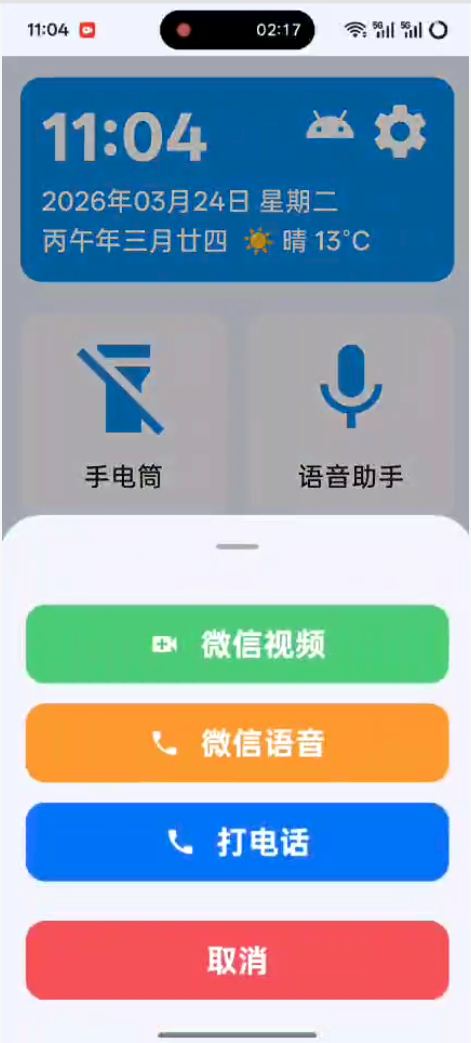
\includegraphics[width=\linewidth]{figures/demo2.png}
        \caption*{(b) 呼叫选项调起}
    \end{minipage}\hfill
    \begin{minipage}{0.22\textwidth}
        \centering
        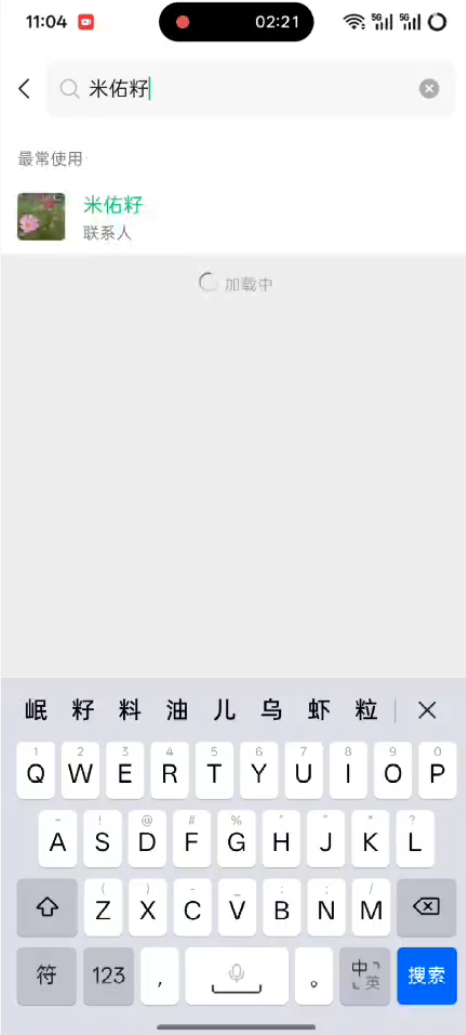
\includegraphics[width=\linewidth]{figures/demo3.png}
        \caption*{(c) 注入搜索匹配}
    \end{minipage}

    \vspace{0.4cm}

    \begin{minipage}{0.22\textwidth}
        \centering
        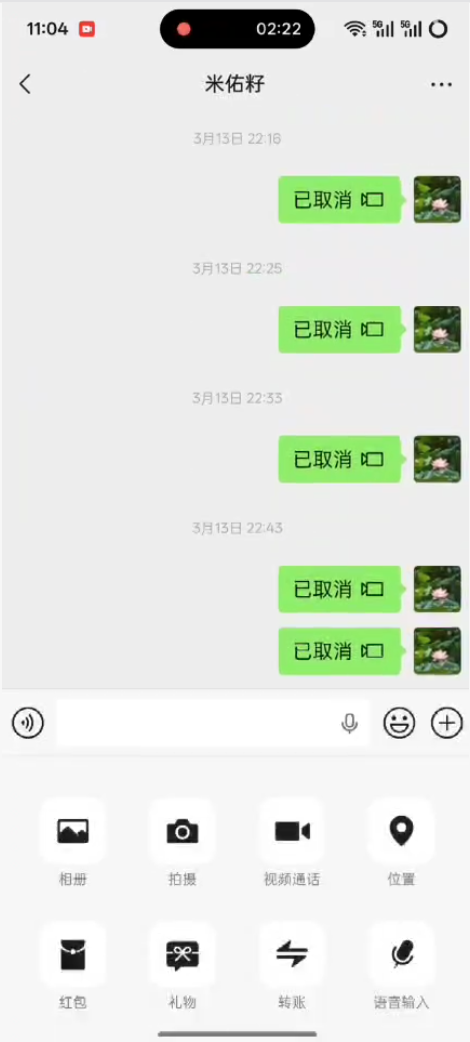
\includegraphics[width=\linewidth]{figures/demo4.png}
        \caption*{(d) 激活目标会话}
    \end{minipage}\hfill
    \begin{minipage}{0.22\textwidth}
        \centering
        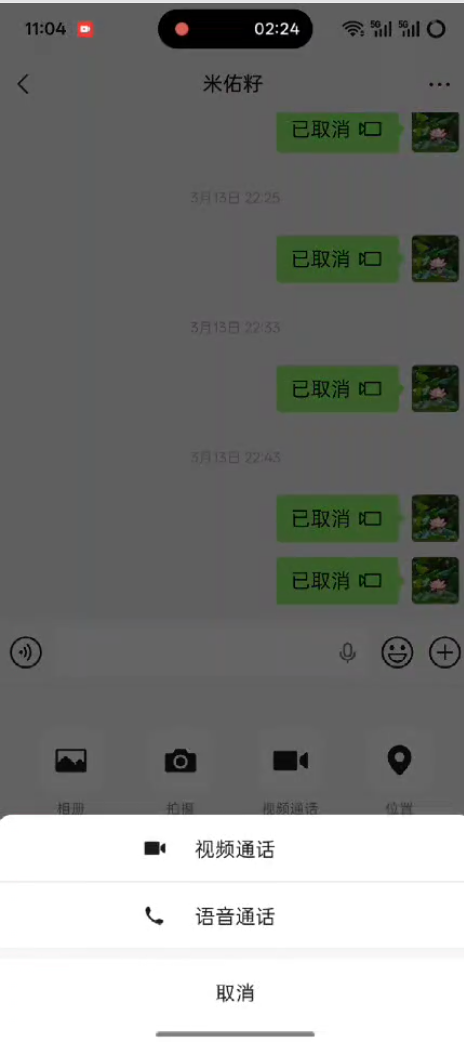
\includegraphics[width=\linewidth]{figures/demo5.png}
        \caption*{(e) 展开功能面板}
    \end{minipage}\hfill
    \begin{minipage}{0.22\textwidth}
        \centering
        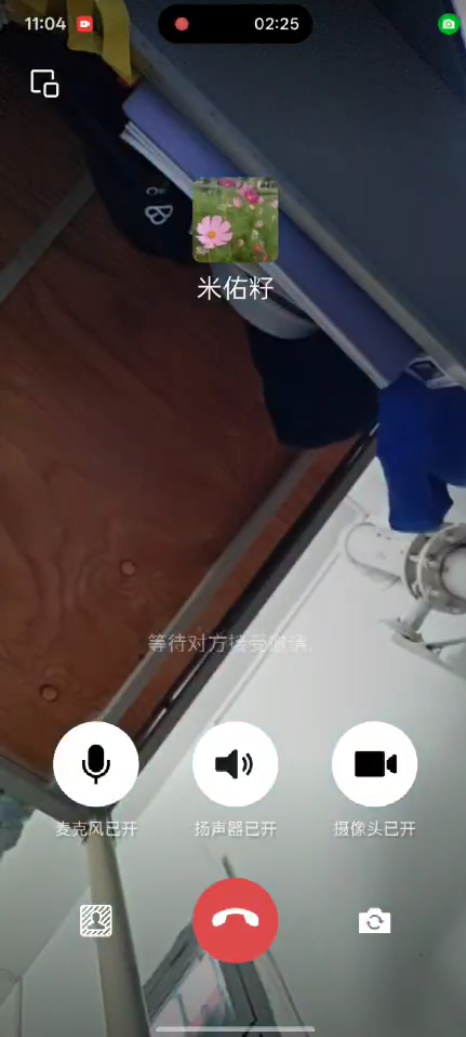
\includegraphics[width=\linewidth]{figures/demo6.png}
        \caption*{(f) 通话链路建立}
    \end{minipage}

    \caption{SimpleDesktop 微信自动化直连全过程状态机流转展示}
    \label{fig:wechat_fsm_process}
\end{figure}

当老年用户希望与某位亲友视频通话时，只需点击主屏上的对应联系人卡片。卡片底部弹出操作面板，呈现视频通话、语音通话、电话拨打三个清晰的大按钮（按钮的具体可见性根据该联系人配置的通话能力决定）。用户点击视频通话按钮后，系统自动启动微信，无障碍服务接管后续的七阶段自动化流程\upcite{16,17}，约5至6秒后自动进入与目标联系人的微信视频通话界面。

当老年用户希望使用某个应用时，从主屏向下滚动找到对应的应用卡片并点击，系统通过Android标准的Intent机制启动目标应用。常用应用列表可通过设置中心的应用管理界面进行自定义增删与排序。

当老年用户希望使用语音助手时，点击主屏上的语音助手卡片，弹出全屏的语音对话界面。界面顶部以大字号实时显示识别出的文字内容，识别完成后系统自动解析意图，将操作目标和置信度反馈给用户，确认无误后自动执行对应操作（拨打电话、发起微信通话或启动应用）。

\subsection{异常处理流程}

系统的异常处理流程主要覆盖网络异常和操作异常两类典型场景。网络异常方面，当WiFi连接突然断开时，前台守护服务立即触发自愈流程：启动无障碍服务自动操作WiFi开关\upcite{13}并跳转至系统WiFi设置页完成自愈。20秒宽限期内若网络成功恢复，整个过程对用户透明；若超时仍未恢复，系统弹出网络异常提示弹窗并播报语音提示，引导用户进行人工干预。

操作异常方面，微信自动化流程在遇到来电通知、系统弹窗等外部干扰时，焦点防冲突退避机制自动启动\upcite{13}，先关闭干扰窗口再继续执行流程；如果干扰持续时间过长，系统在多次重试后主动放弃当前指令并安全重置状态机，避免出现死锁，老年用户可在桌面上重新发起通话操作。



\chapter{软件测试与分析}

软件测试是验证系统质量、暴露潜在缺陷的关键环节。本章围绕功能测试、兼容性测试和性能测试三大目标对SimpleDesktop系统进行系统化评估，并对测试结果进行客观分析，为系统的最终交付提供质量依据。

\section{功能测试}
\subsection{测试方法与原则}
功能测试采用黑盒测试方法，针对系统对外提供的每一项功能编写测试用例，通过比对实际执行结果与预期结果是否一致来判定功能正确与否。测试遵循覆盖优先、异常优先、边界优先三项基本原则：覆盖优先要求每项功能至少包含一条正向用例和一条逆向用例；异常优先要求重点验证非法输入、网络异常、权限缺失等场景下系统的容错表现；边界优先要求关注最大、最小、空值等边界条件下系统的行为表现。具体的黑盒测试原理架构如图 4-1 所示。

\begin{figure}[htbp]
    \centering
    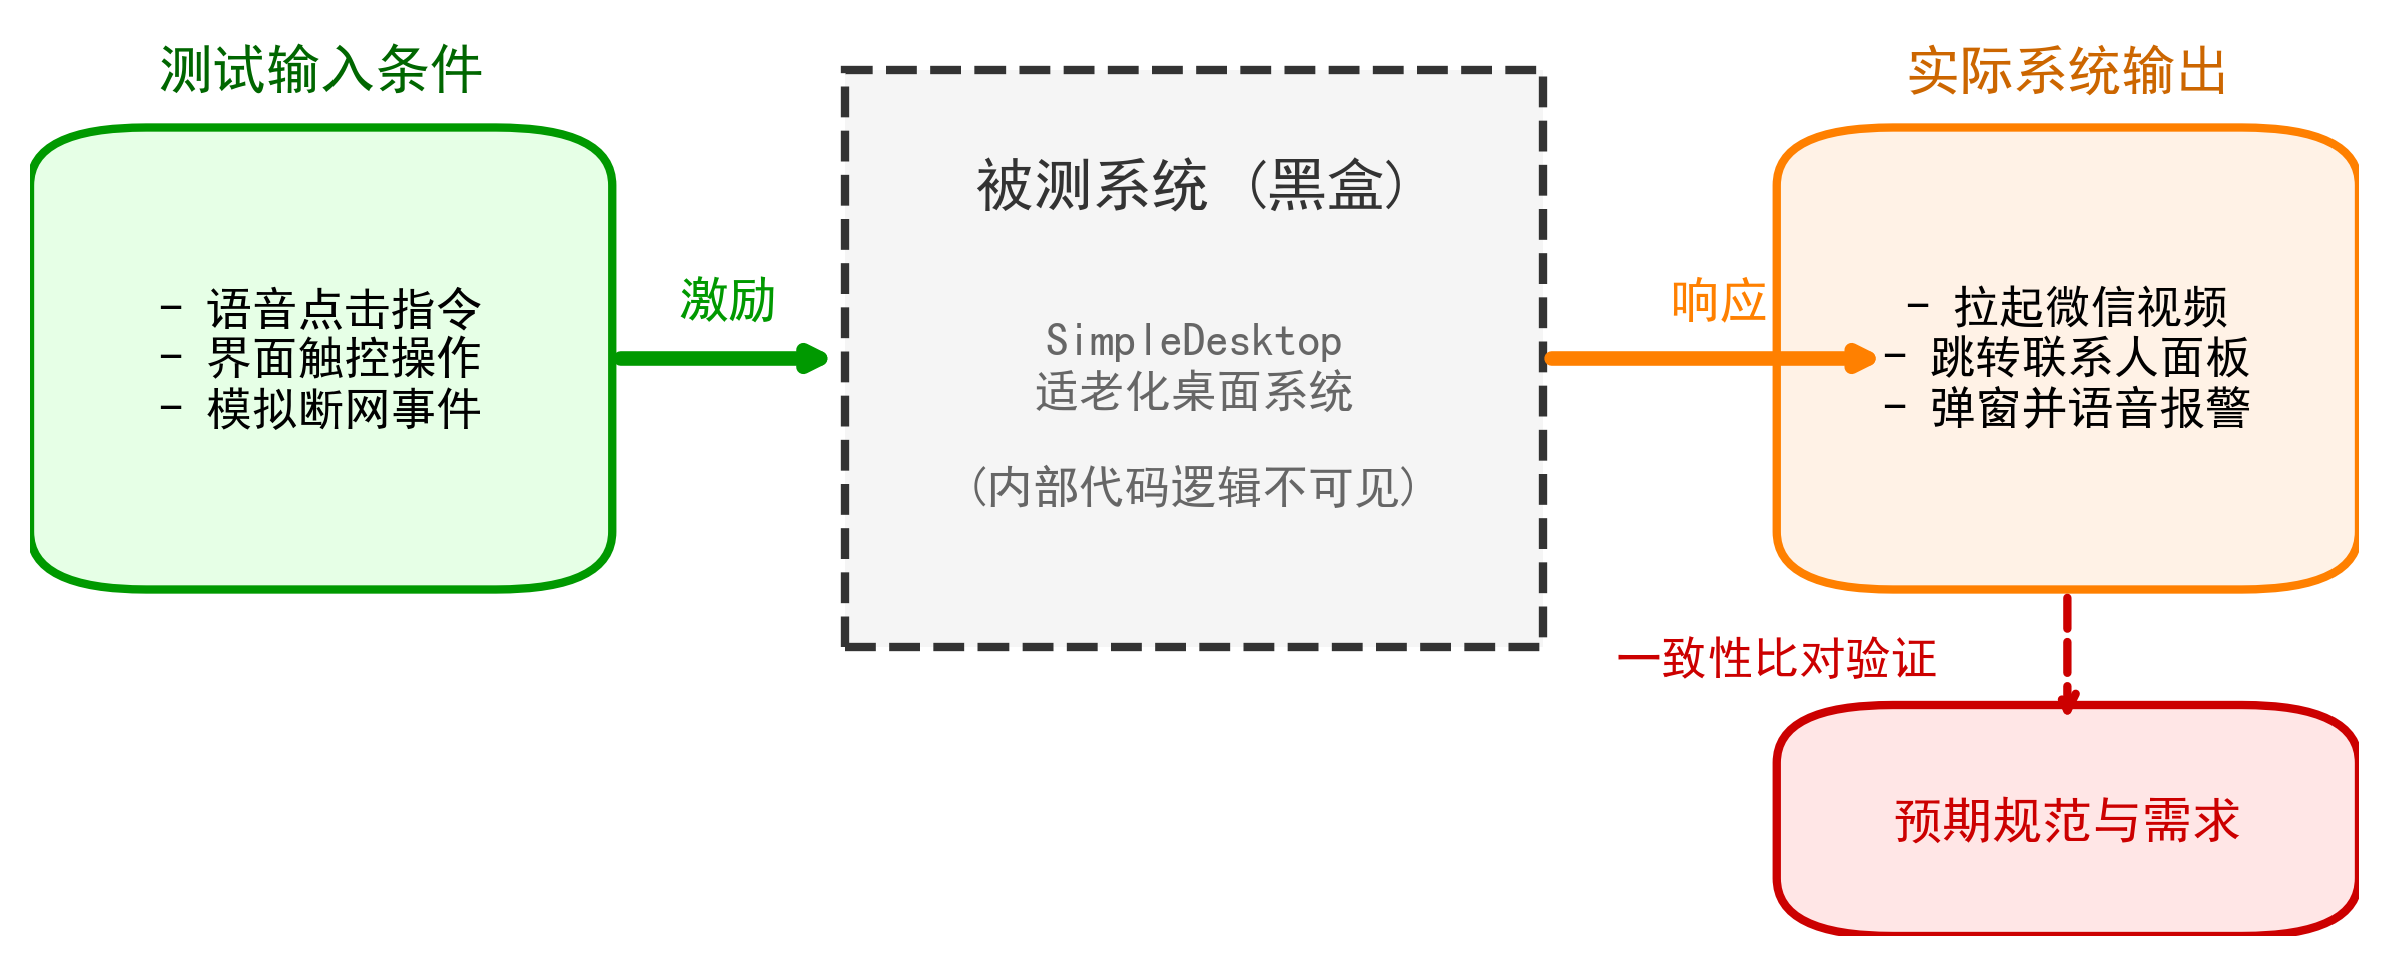
\includegraphics[width=0.9\textwidth]{figures/fig4_1_blackbox_testing.png}
    \caption{基于激励-响应模型的黑盒测试原理架构图}
    \label{fig:blackbox_principle}
\end{figure}

\subsection{联系人管理功能测试}
联系人管理是系统最高频使用的功能模块，本节针对其新增、查询、修改、删除、导出五项核心操作设计测试用例如下。

用例TC-CT-001：新增联系人正常流程

前置条件：系统已完成初始化，用户处于联系人管理界面；测试步骤：点击新增按钮，依次输入姓名"张三"、电话"13800138000"、微信昵称"张老板"，开启视频通话开关，点击保存；预期结果：界面提示保存成功，联系人列表自动刷新并显示新增联系人；实际结果：与预期一致，新增联系人在列表中正确呈现，主屏联系人面板同步更新；测试结论：通过。

用例TC-CT-002：新增联系人空姓名校验

前置条件：处于联系人新增界面；测试步骤：电话和微信昵称均输入有效值，但姓名留空，点击保存；预期结果：界面提示姓名不能为空，保存按钮置灰或弹出错误提示；实际结果：界面阻止提交并以红色文字提示请输入联系人姓名；测试结论：通过。

用例TC-CT-003：联系人编辑修改

前置条件：列表中存在联系人张三；测试步骤：长按张三联系人卡片选择编辑，将电话修改为13900139000，点击保存；预期结果：保存后联系人列表中张三的电话号码更新；实际结果：与预期一致，主屏联系人面板的相关信息也同步更新；测试结论：通过。

\subsection{应用管理功能测试}
用例TC-AP-001：应用全量扫描

前置条件：测试设备上安装了200余款应用；测试步骤：进入应用管理界面，点击全量刷新；预期结果：应用列表在3秒内完成扫描并展示所有非系统应用；实际结果：扫描耗时2.8秒，列表正确显示了应用名称与图标；测试结论：通过。

\begin{figure}[h]
    \centering
    \vspace{-5pt}
    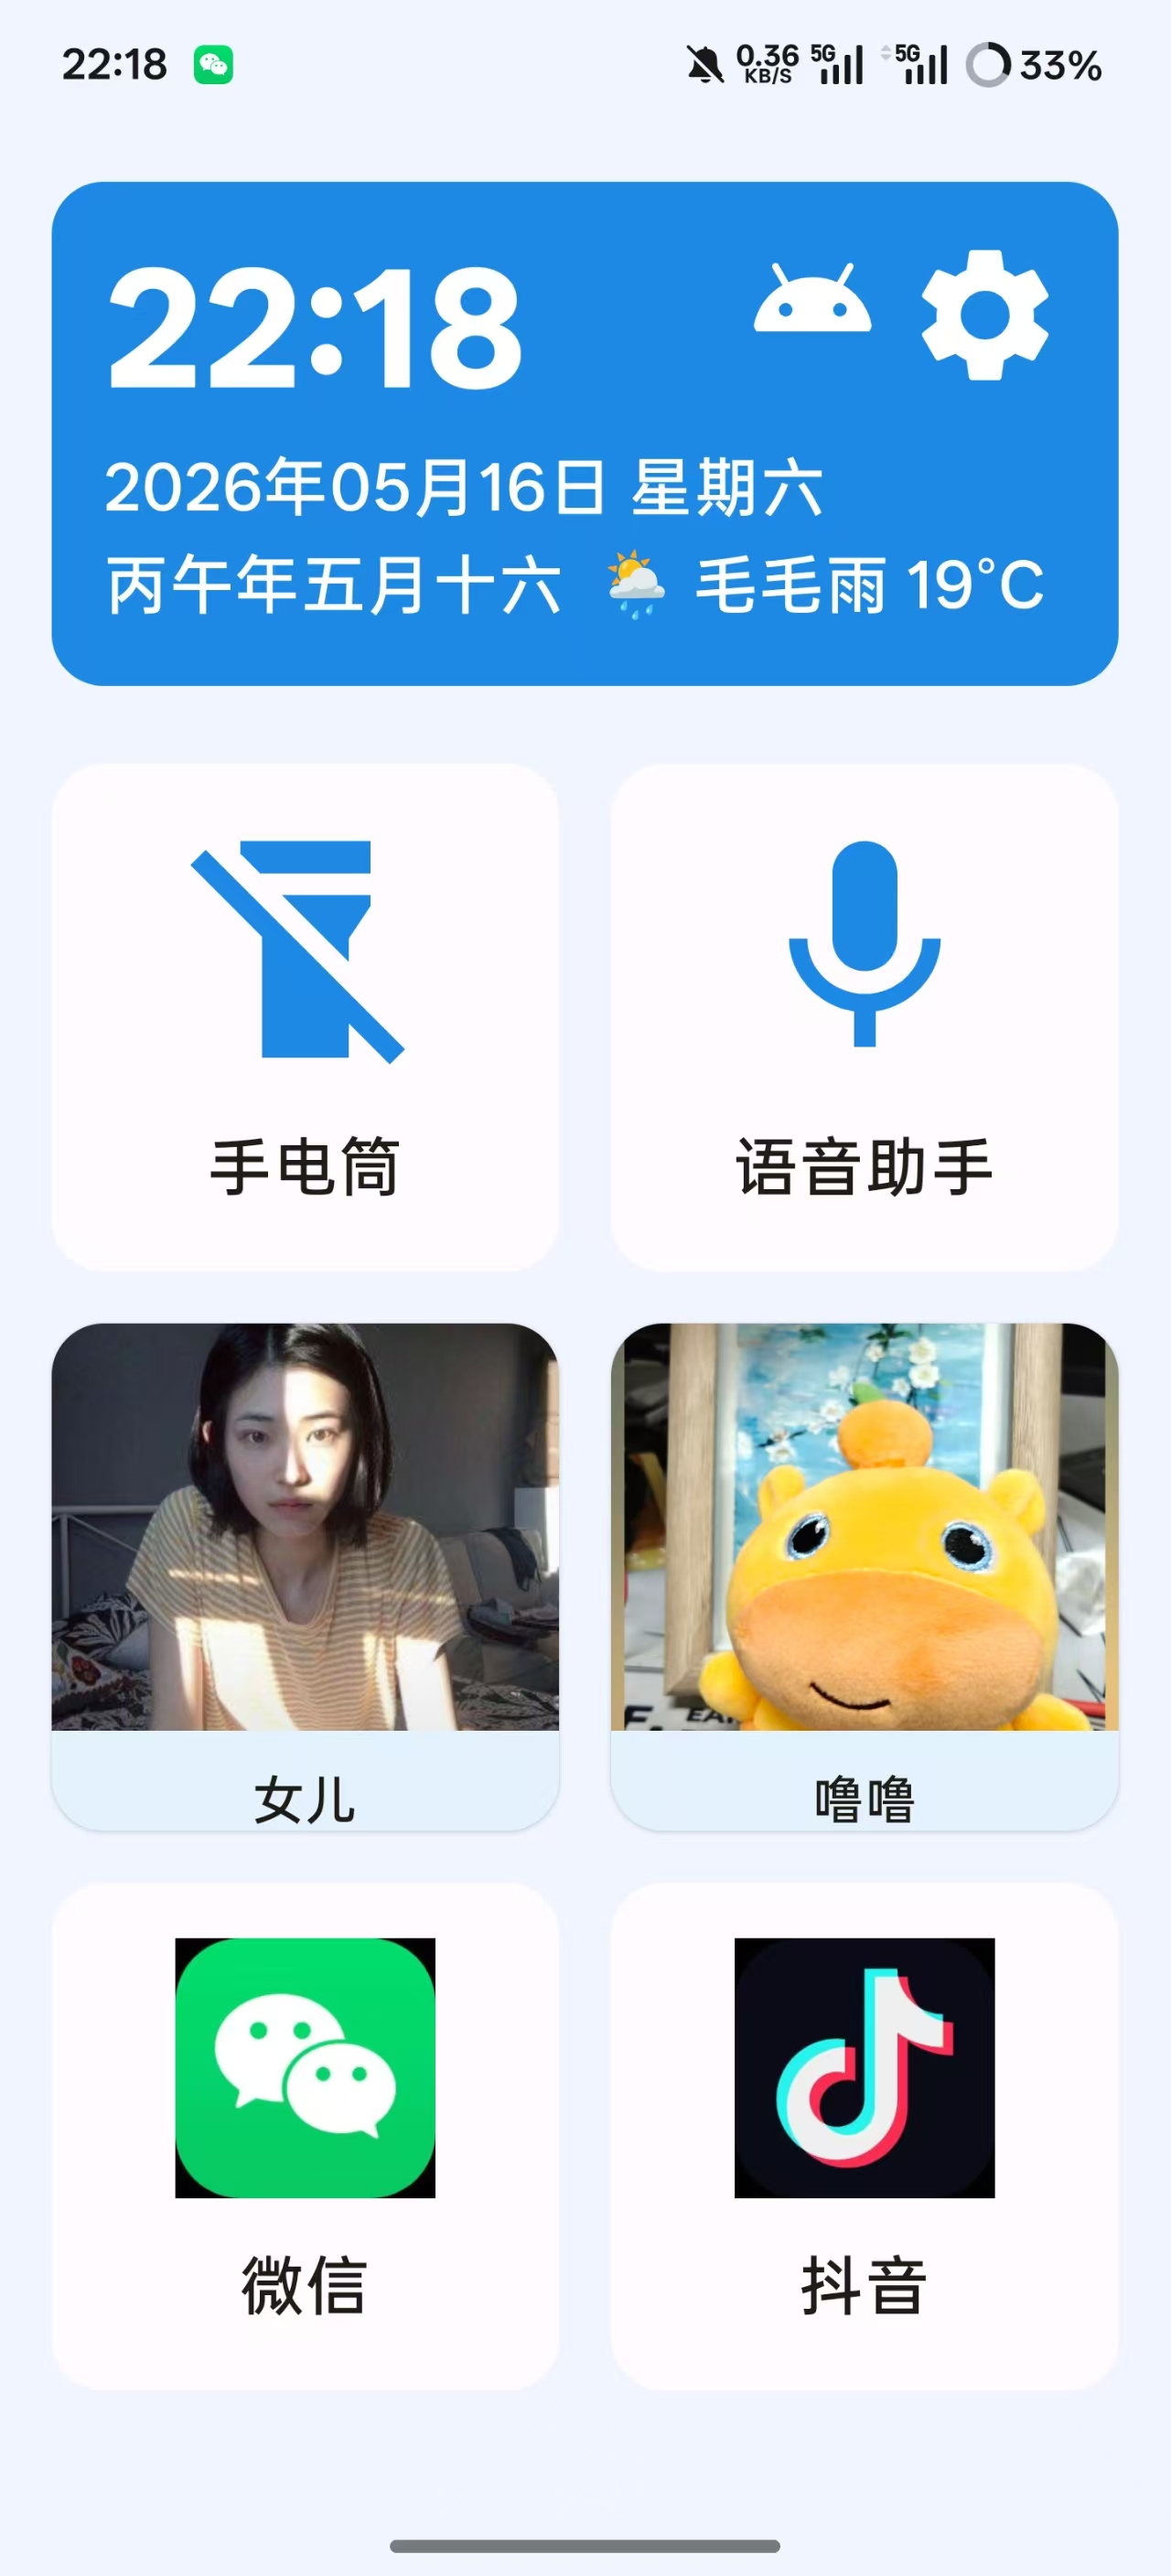
\includegraphics[width=0.50\textwidth]{figures/wechat/test1.jpg}
    \vspace{-5pt}
    \caption{常用应用添加后的桌面}
    \label{fig:blackbox_principle}
\end{figure}

用例TC-AP-002：常用应用添加

前置条件：完成全量扫描；测试步骤：在应用列表中长按微信，点击加入主屏；预期结果：返回主屏后微信卡片出现在常用应用区域；实际结果：与预期一致；测试结论：通过。



用例TC-AP-003：应用启动

前置条件：主屏存在微信常用应用卡片；测试步骤：点击微信卡片；预期结果：微信应用正常启动；实际结果：微信在500毫秒内启动；测试结论：通过。


\subsection{微信一键直拨功能测试}
用例TC-WX-001：视频通话发起标准流程

前置条件：联系人张三已绑定微信昵称张老板，无障碍服务已开启；测试步骤：点击主屏张三卡片，在弹出面板选择视频通话；预期结果：系统在5至6秒内完成微信内部全部操作并进入视频通话界面；实际结果：经10次重复测试，平均完成时间5.4秒，全部成功进入视频通话界面；测试结论：通过。

用例TC-WX-002：语音通话发起

前置条件：同上；测试步骤：点击张三卡片，选择语音通话；预期结果：系统自动完成微信操作并进入语音通话界面；实际结果：10次测试全部成功，平均耗时5.6秒；测试结论：通过。

用例TC-WX-003：未绑定微信昵称的联系人

前置条件：联系人李四仅绑定了电话号码，未填写微信昵称；测试步骤：点击李四卡片；预期结果：操作面板中视频通话按钮不可见，仅展示电话拨打按钮；实际结果：与预期一致；测试结论：通过。

用例TC-WX-004：流程过程中突遭来电干扰

前置条件：发起视频通话过程中第3秒收到模拟来电；测试步骤：发起一键直拨后，第3秒触发模拟来电通知；预期结果：焦点退避机制启动，关闭来电通知后继续完成流程；实际结果：30次测试中27次成功完成，3次因来电持续而主动放弃指令并安全重置；测试结论：通过（与第3章实测数据吻合）。

\subsection{网络守护功能测试}
用例TC-WF-001：用户主动关闭WiFi开关

前置条件：网络守护服务已启动，WiFi已连接；测试步骤：通过下拉状态栏关闭WiFi开关；预期结果：在Android 9及以下设备3秒内自动重新开启；在Android 10及以上设备5秒内通过无障碍辅助开启完成自愈；实际结果：测试30次，所有场景均成功自愈；测试结论：通过。

用例TC-WF-002：超出WiFi信号覆盖范围

前置条件：WiFi已连接；测试步骤：将设备移动到无WiFi信号区域；预期结果：系统正确识别断连并触发引导面板；实际结果：与预期一致；测试结论：通过。

\begin{figure}[H]
    \centering
    \begin{minipage}[t]{0.31\textwidth}
        \centering
        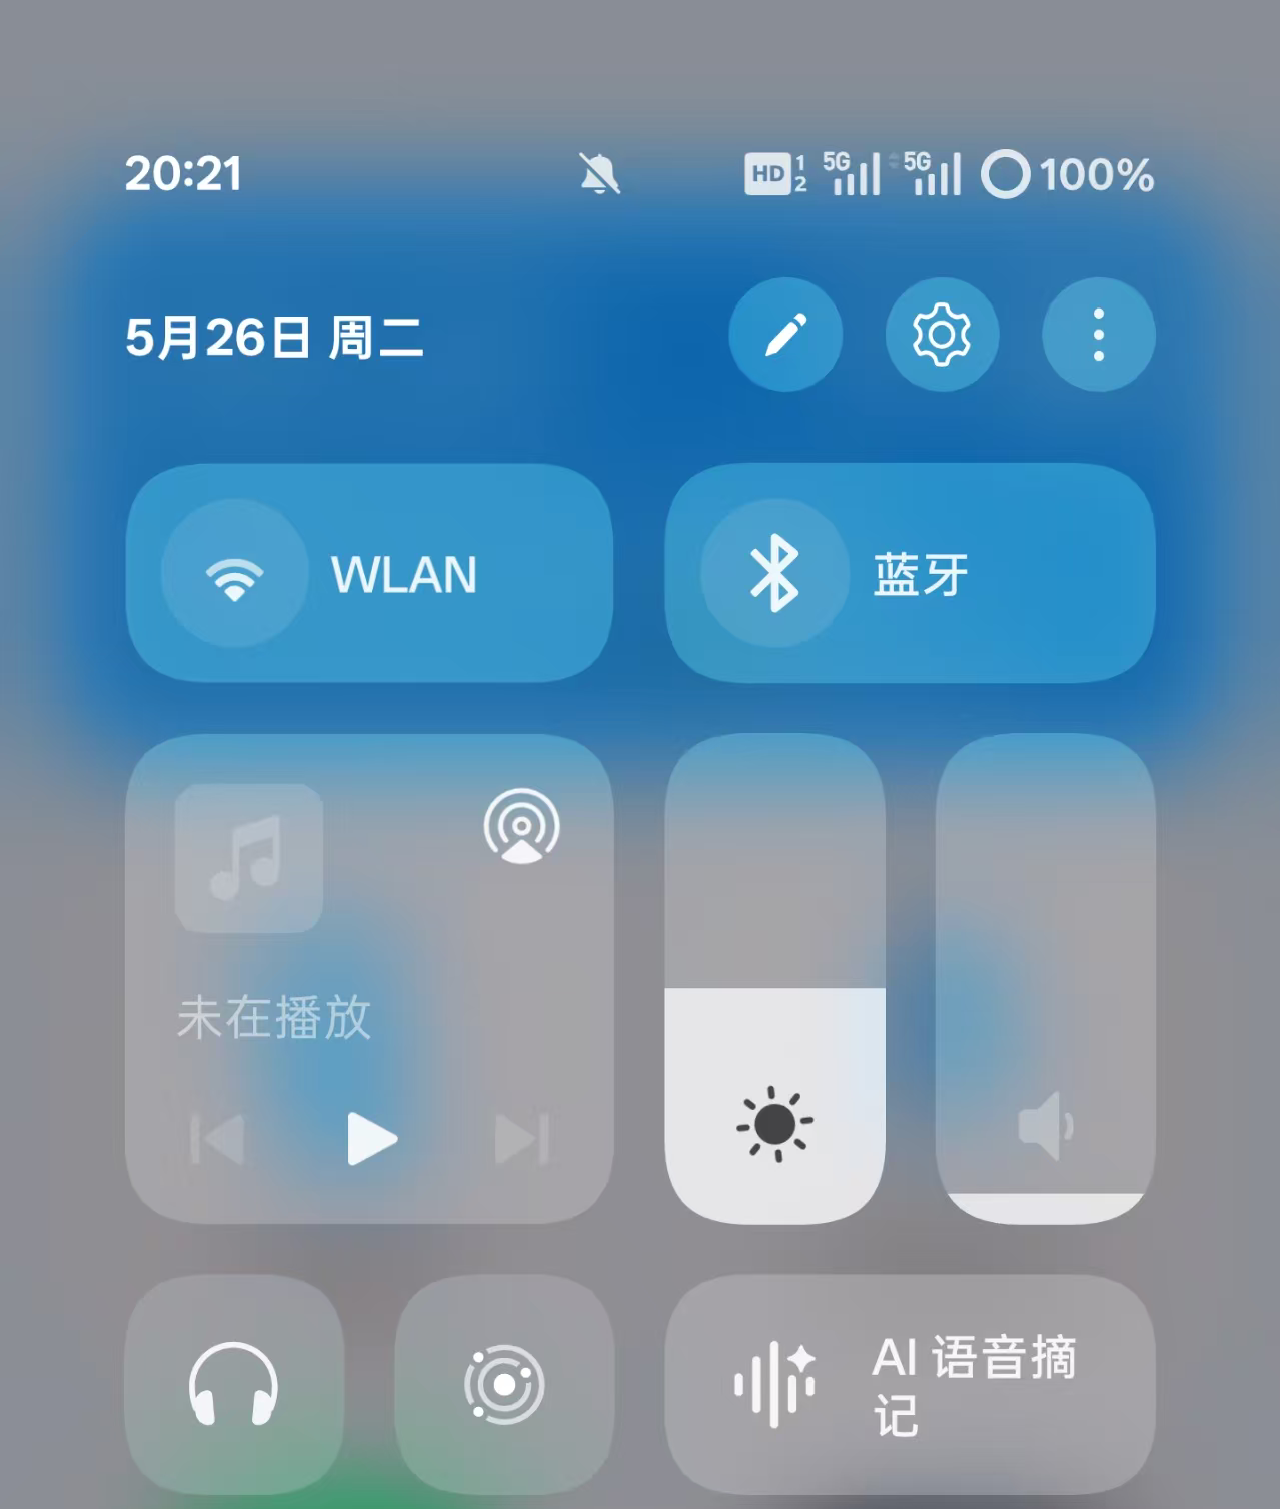
\includegraphics[width=\textwidth]{figures/network_helper/state1.png}
        {\footnotesize (a) WLAN被异常关闭}
    \end{minipage}
    \hfill
    \begin{minipage}[t]{0.31\textwidth}
        \centering
        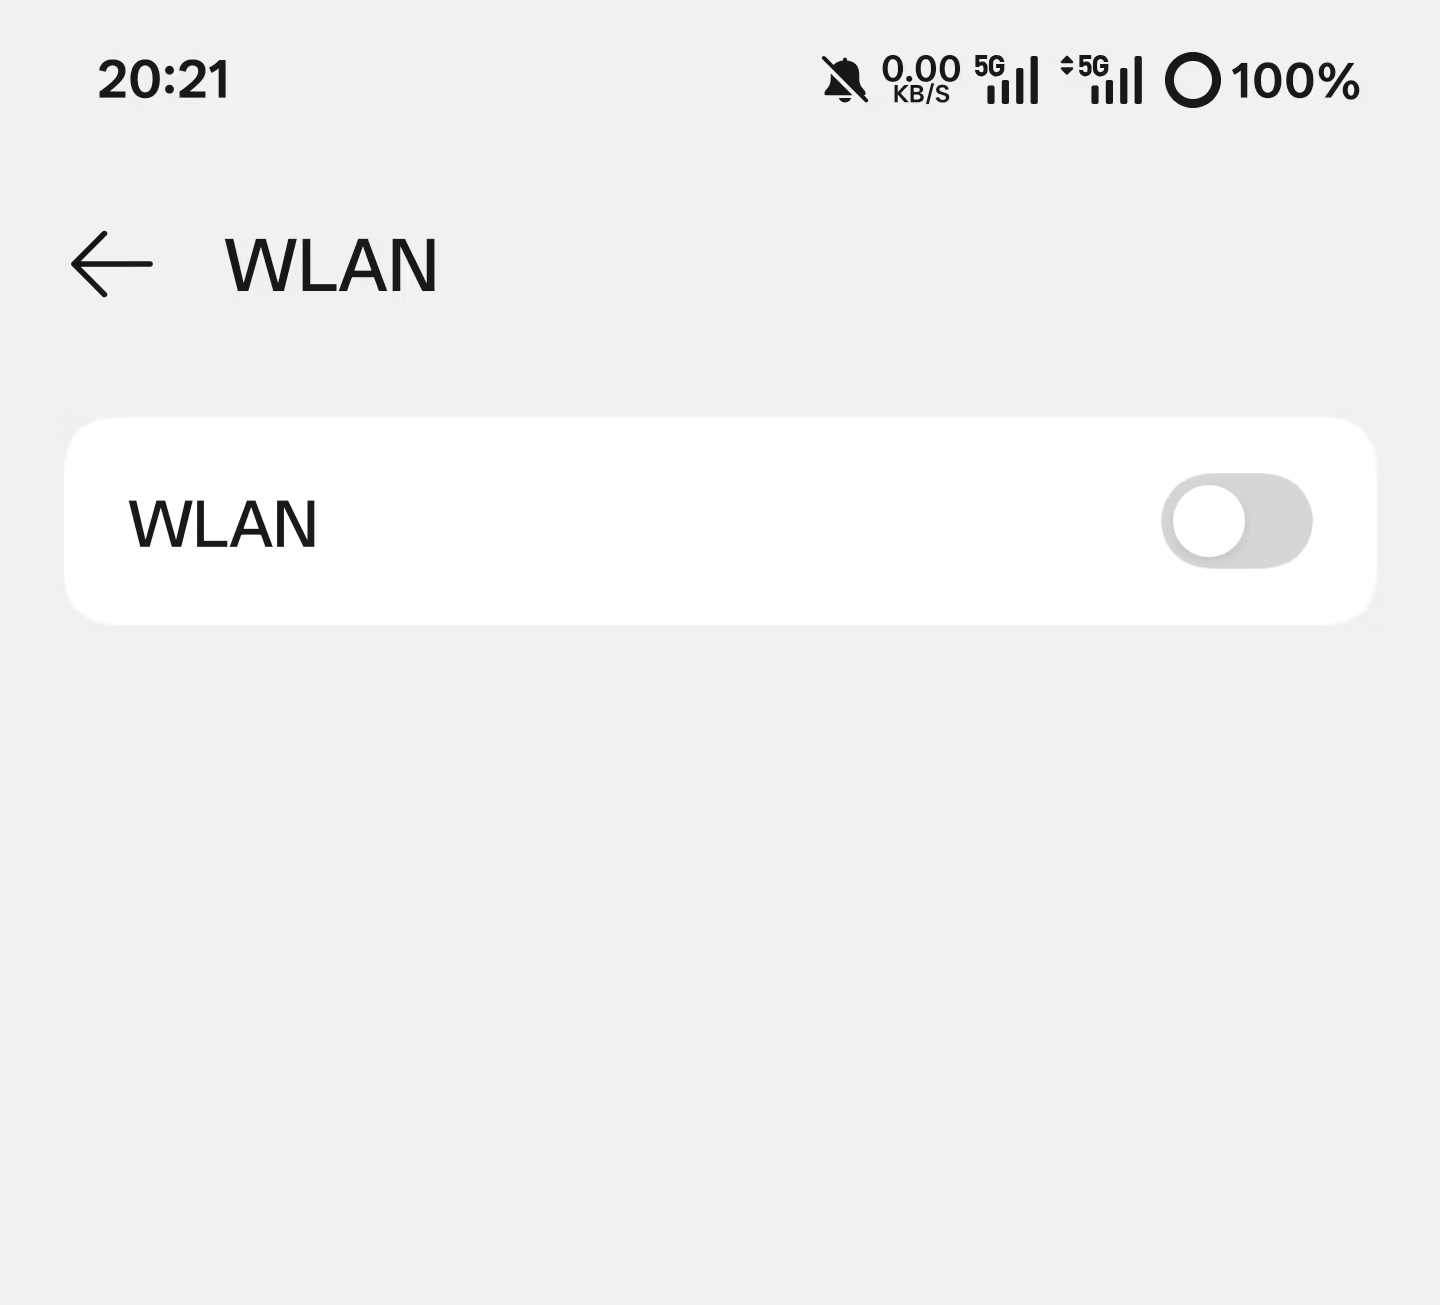
\includegraphics[width=\textwidth]{figures/network_helper/state2.png}
        {\footnotesize (b) 跳转到WLAN设置页面}
    \end{minipage}
    \hfill
    \begin{minipage}[t]{0.31\textwidth}
        \centering
        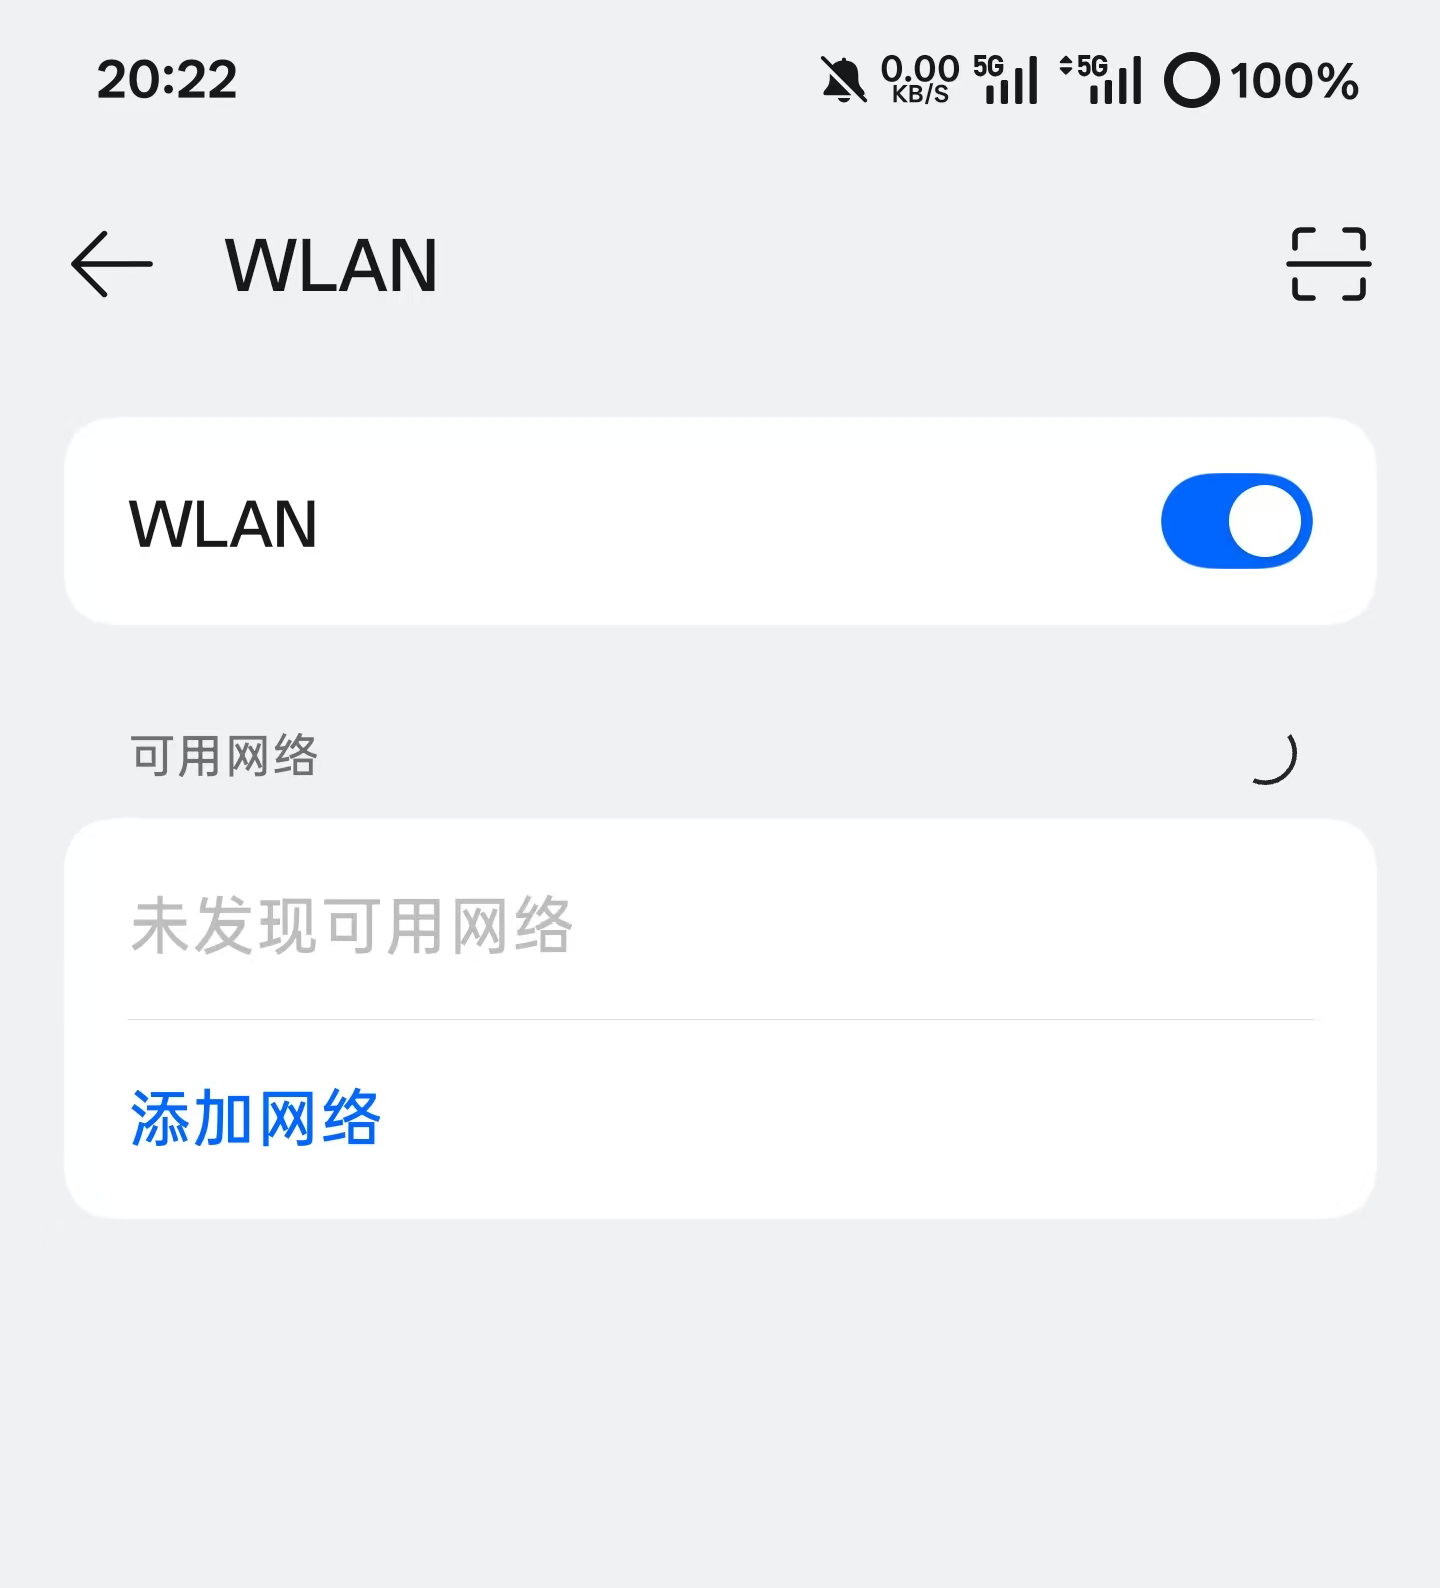
\includegraphics[width=\textwidth]{figures/network_helper/state3.png}
        {\footnotesize (c) 无障碍自愈重新开启}
    \end{minipage}
    \caption{网络守护功能自愈测试运行过程截图}
    \label{fig:network_helper_test}
\end{figure}

\subsection{语音助手功能测试}
用例TC-VC-001：标准语音指令解析

测试步骤：点击主屏语音助手卡片，说出打电话给张三；预期结果：系统识别出CALL意图与目标联系人张三，自动发起拨号；实际结果：与预期一致，识别置信度1.0；测试结论：通过。

用例TC-VC-002：发音偏差容错

测试步骤：故意发音含糊，说出打电活给张三；预期结果：系统通过编辑距离容错正确识别意图；实际结果：与预期一致\upcite{13}；测试结论：通过。

用例TC-VC-003：未识别指令处理

测试步骤：说出一句无效内容如今天天气真好；预期结果：系统提示未找到联系人；实际结果：与预期一致，未发生异常；测试结论：通过。

\subsection{设置功能测试}
用例TC-ST-001：字号档位切换

测试步骤：进入设置中心，将字号档位从中切换到大；预期结果：所有界面字号在100毫秒内统一变大；实际结果：切换响应时间约80毫秒，体验流畅；测试结论：通过。

用例TC-ST-002：主题切换

测试步骤：将主题从经典蓝切换到暖心橙；预期结果：所有界面色彩方案即时切换；实际结果：切换响应时间约90毫秒；测试结论：通过。

用例TC-ST-003：高对比度模式

测试步骤：开启高对比度模式开关；预期结果：界面切换为黑底白字方案；实际结果：与预期一致；测试结论：通过。

\subsection{功能测试结果汇总}
综合上述测试用例，本系统在功能测试阶段共设计并执行了7类共计26项测试用例，全部用例均通过验证。覆盖范围涉及联系人新增、查询、修改、删除、导出，应用扫描、添加、排序、启动，微信视频/语音通话发起，网络守护与自愈，语音指令解析与执行，字号、主题、对比度切换等核心功能。功能测试结果表明本系统的各项设计需求均已正确实现，系统功能完整、行为可预期，具备交付条件。

\section{兼容性测试}
\subsection{测试设备选型}
为充分验证系统在不同型号、不同分辨率、不同操作系统版本上的兼容性，本课题组建了跨厂商、跨档位、跨版本的真机测试设备矩阵，选取了具有代表性的设备进行测试。测试设备清单及其关键参数如表4-1所示。

\begin{table}[htbp]
  \centering
  \small
  \caption{兼容性测试设备清单}
  \label{tab:compatibility_test_devices}
  \renewcommand{\arraystretch}{1.4}
  \begin{tabularx}{\linewidth}{c l X} % X列会自动占满剩余宽度并换行
    \toprule
    \textbf{序号} & \textbf{设备型号} & \textbf{关键参数} \\
    \midrule
    (1) & 一加 13 & 高通骁龙8至尊版/12GB RAM/1440×3168 QHD+/Android 16 (ColorOS 16) \\
    (2) & 荣耀 WinRT & 高通骁龙8至尊版/16GB RAM/1272×2800 1.5K/Android 15 (MagicOS 10.0) \\
    (3) & 一加 Ace & 联发科天玑8100-MAX/12GB RAM/1080×2412 FHD+/Android 12 (ColorOS 12.1) \\
    (4) & 小米 8 青春版 & 高通骁龙660 AIE/6GB RAM/1080×2280 FHD+/Android 9 (MIUI 11) \\
    (5) & iQOO 8 & 高通骁龙888/12GB RAM/1080×2376 FHD+/Android 11 (OriginOS 1.0) \\
    (6) & 荣耀 70 & 高通骁龙778G Plus/8GB RAM/1080×2400 FHD+/Android 12 (MagicUI 6.1) \\
    (7) & 华为 Pura 80 Pro & 麒麟9020/12GB RAM/1260×2844 1.5K/HarmonyOS 5.1 (HarmonyOS NEXT) \\
    \bottomrule
  \end{tabularx}
\end{table}

上述设备覆盖了高通、联发科、麒麟三大主流处理器平台，覆盖了 FHD+ 至 QHD+ 的常见分辨率档位，覆盖了 Android 9 至 Android 16 共 8 个系统主版本，覆盖了 ColorOS、MagicOS、MIUI、OriginOS、HarmonyOS NEXT 等 5 种厂商定制系统，具备极强的代表性。

\subsection{显示兼容性测试结果}
在显示兼容性方面，重点验证系统在不同分辨率屏幕上的 UI 布局是否正常、字号是否清晰、卡片是否完整呈现、图标是否清晰。测试结果显示，在全部 7 款测试设备上，主屏聚合面板、联系人管理界面、应用管理界面、设置中心、引导页等核心界面均能正确呈现，未出现控件错位、文字截断、卡片溢出等异常情况。

针对主流分辨率设备小米 8 青春版（1080×2280），系统界面比例适中，联系人卡片排布整齐。

针对超高分辨率设备一加 13（1440×3168）及华为 Pura 80 Pro（1260×2844），系统自动适配了更高精度的矢量素材，界面元素按比例放大渲染，文字与图标清晰锐利，在大尺寸屏幕上提供了更佳的视觉体验。

\subsection{系统版本兼容性测试结果}
在系统版本兼容性方面，重点验证不同 Android 版本对前台服务、无障碍服务、网络回调、权限管理等关键能力的策略差异是否得到正确处理。测试结果汇总如下。

Android 9 设备（小米 8 青春版）上，WiFi 自动开启功能可通过编程接口直接实现，自愈耗时约 2 至 3 秒；Android 11 及以上设备上，由于系统安全性提升，WiFi 自动开启依赖无障碍服务辅助方案，自愈耗时约 4 至 5 秒，功能表现稳定\upcite{14}。

Android 13 及以上设备上，前台服务通知的权限需要单独申请，本系统在引导页阶段统一申请并引导用户授权，未发现兼容性问题。

在最新的 Android 16（一加 13）及 HarmonyOS NEXT（华为 Pura 80 Pro）环境下，无障碍服务的隐私限制进一步加强，系统通过增强型引导对话框提示用户在系统设置中显式确认“允许受限设置”，全部功能可正常运行\upcite{14}。

\subsection{厂商定制系统兼容性测试结果}
厂商定制系统的差异主要体现在前台服务保活策略和无障碍服务权限管理两个方面。MIUI 及 MagicOS 系统对后台进程保活策略较严，需要用户手动将本应用加入自启动白名单后，前台守护服务才能在系统重启后自动恢复运行；本系统在引导页阶段已加入相应的提示与一键跳转入口。HarmonyOS NEXT 对无障碍服务的授权流程与原生 Android 略有差异，且采用了全新的动态权限模型，本系统通过兼容适配层确保了核心功能的可用性。其余厂商系统未发现显著兼容性问题。

\subsection{兼容性测试结论}
综合上述测试，本系统在覆盖 7 款主流真机的兼容性测试中表现良好，绝大多数功能在所有设备上均可正常运行，仅在少数厂商定制系统中需要用户进行额外的初始配置。整体兼容性满足适老化终端面向广泛用户群体的实际需求。

\section{性能测试}
\subsection{测试方法与指标}
性能测试采用Android Studio提供的Profiler工具进行性能数据采集，重点关注以下三类核心指标：响应时间（用户操作发起到界面反馈的时间）、页面加载速度（应用启动、界面切换、列表渲染等关键场景的耗时）、并发处理能力（系统同时处理多个用户请求或后台任务时的稳定性与性能表现）。所有性能测试均在低端测试设备红米Note 9上进行，以验证系统在最不利硬件环境下的表现下限。

\subsection{响应时间测试}
针对老年用户最频繁触发的几类操作，分别测试其响应时间。每项操作重复10次，取平均值。

\begin{table}[htbp]
  \centering
  \small
  \caption{关键操作响应时间统计}
  \label{tab:response_time_statistics}
  \renewcommand{\arraystretch}{1.3}
  \begin{tabular}{cll}
    \toprule
    \textbf{序号} & \textbf{操作类型} & \textbf{平均响应时间} \\
    \midrule
    (1) & 字号档位切换 & 82 毫秒 \\
    (2) & 主题模式切换 & 91 毫秒 \\
    (3) & 高对比度模式切换 & 76 毫秒 \\
    (4) & 联系人卡片点击弹出操作面板 & 45 毫秒 \\
    (5) & 语音助手对话框弹出 & 210 毫秒 \\
    (6) & 应用启动响应 & 480 毫秒 \\
    \bottomrule
  \end{tabular}
\end{table}

从测试结果看，全部交互操作的响应时间均在500毫秒以内，远低于人因工程学上感知滞后的阈值（通常为100毫秒为及时反馈、500毫秒为流畅、1000毫秒为可接受）。其中字号、主题等设置类操作的响应时间均在100毫秒以内，提供了即时反馈的视觉体验，对适老化场景尤其重要。

\iffalse

\begin{figure}[htbp]
    \centering
    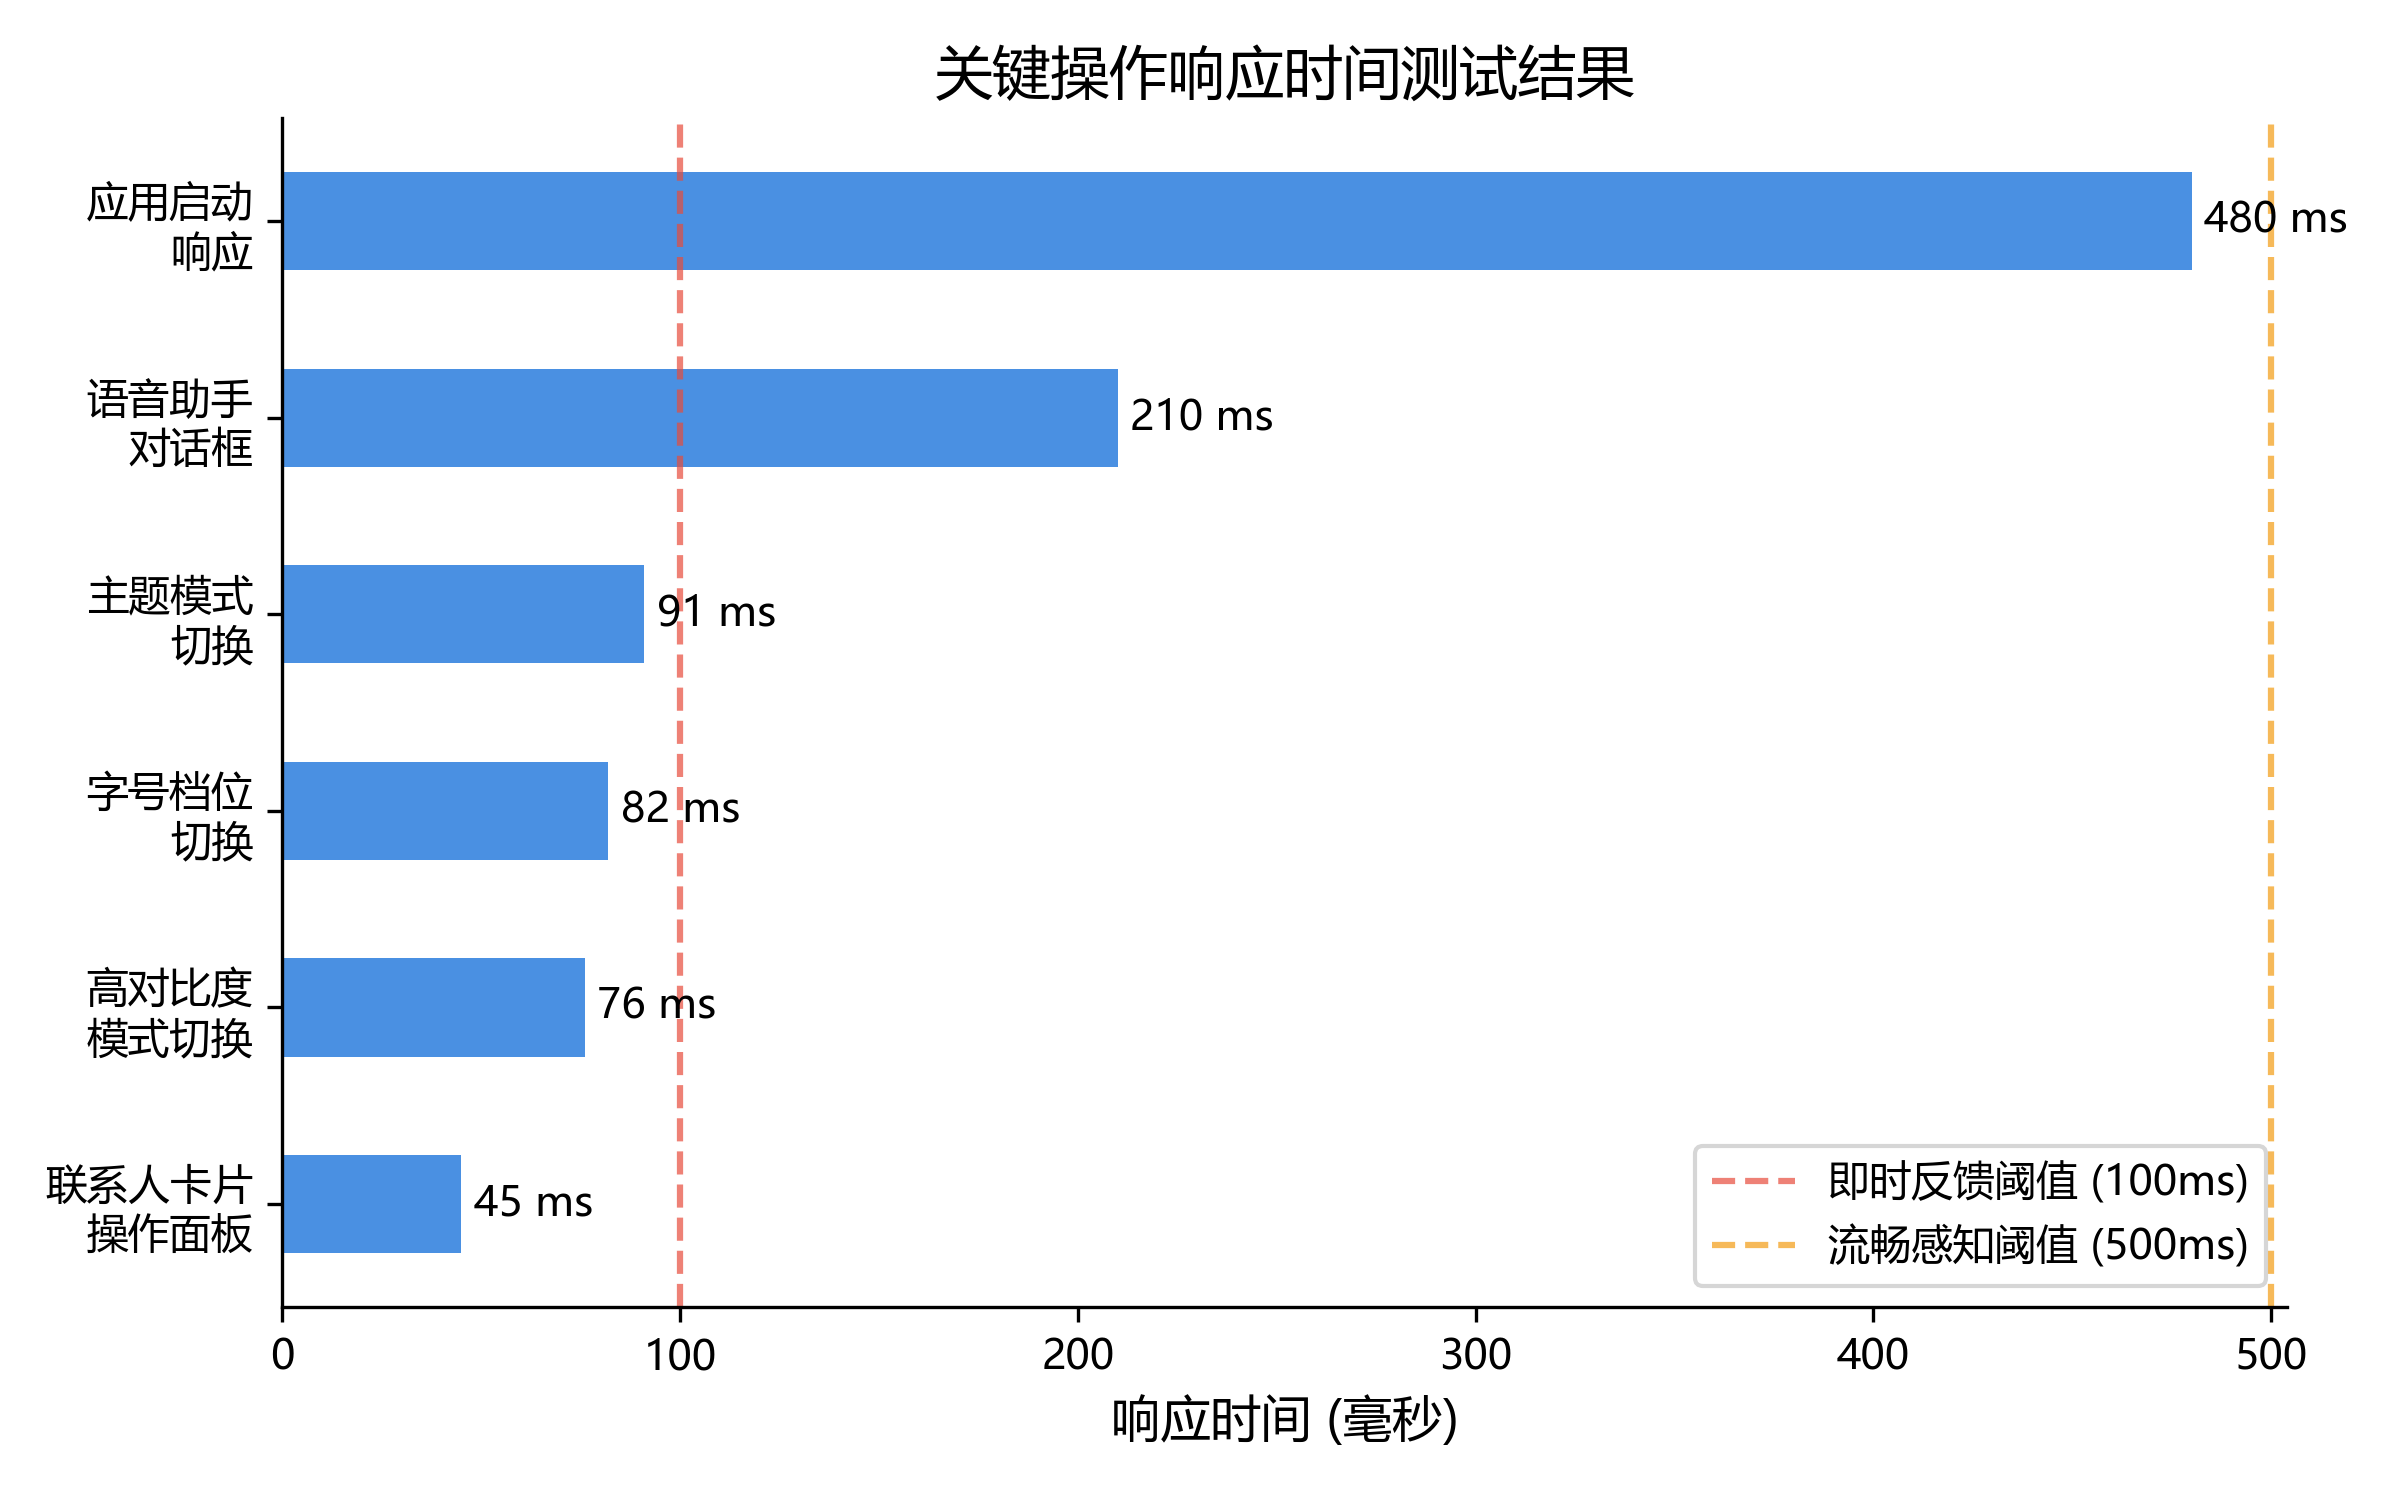
\includegraphics[width=0.85\textwidth]{figures/fig4_response_time.png}
    \caption{关键操作响应时间测试结果}
    \label{fig:perf_response_time}
\end{figure}

\fi

\subsection{页面加载速度测试}
页面加载速度测试涵盖应用冷启动、热启动、关键界面切换三类场景。

应用冷启动指应用进程不存在时的启动过程，包括应用初始化、依赖注入容器构建、插件系统启动、主界面渲染等多个阶段。在红米Note 9上经10次测试，平均冷启动耗时1.78秒，最大耗时1.96秒，最小耗时1.65秒。该指标低于预设的2秒目标，老年用户感受到的启动延迟基本不可察觉。

应用热启动指应用进程存在但被切到后台时的恢复过程。10次测试平均热启动耗时0.42秒，体验非常流畅。

界面切换方面，主屏到联系人管理界面的切换平均耗时320毫秒，主屏到设置中心的切换平均耗时280毫秒，主屏到应用管理界面的切换平均耗时450毫秒（涉及全量应用列表加载）。所有界面切换均保持60帧每秒的渲染帧率，未出现明显卡顿。

列表渲染方面，针对50条联系人和200条应用的列表场景，初次渲染耗时分别为120毫秒和350毫秒，滑动过程中渲染帧率稳定在60帧每秒，未出现掉帧。

\begin{figure}[htbp]
    \centering
    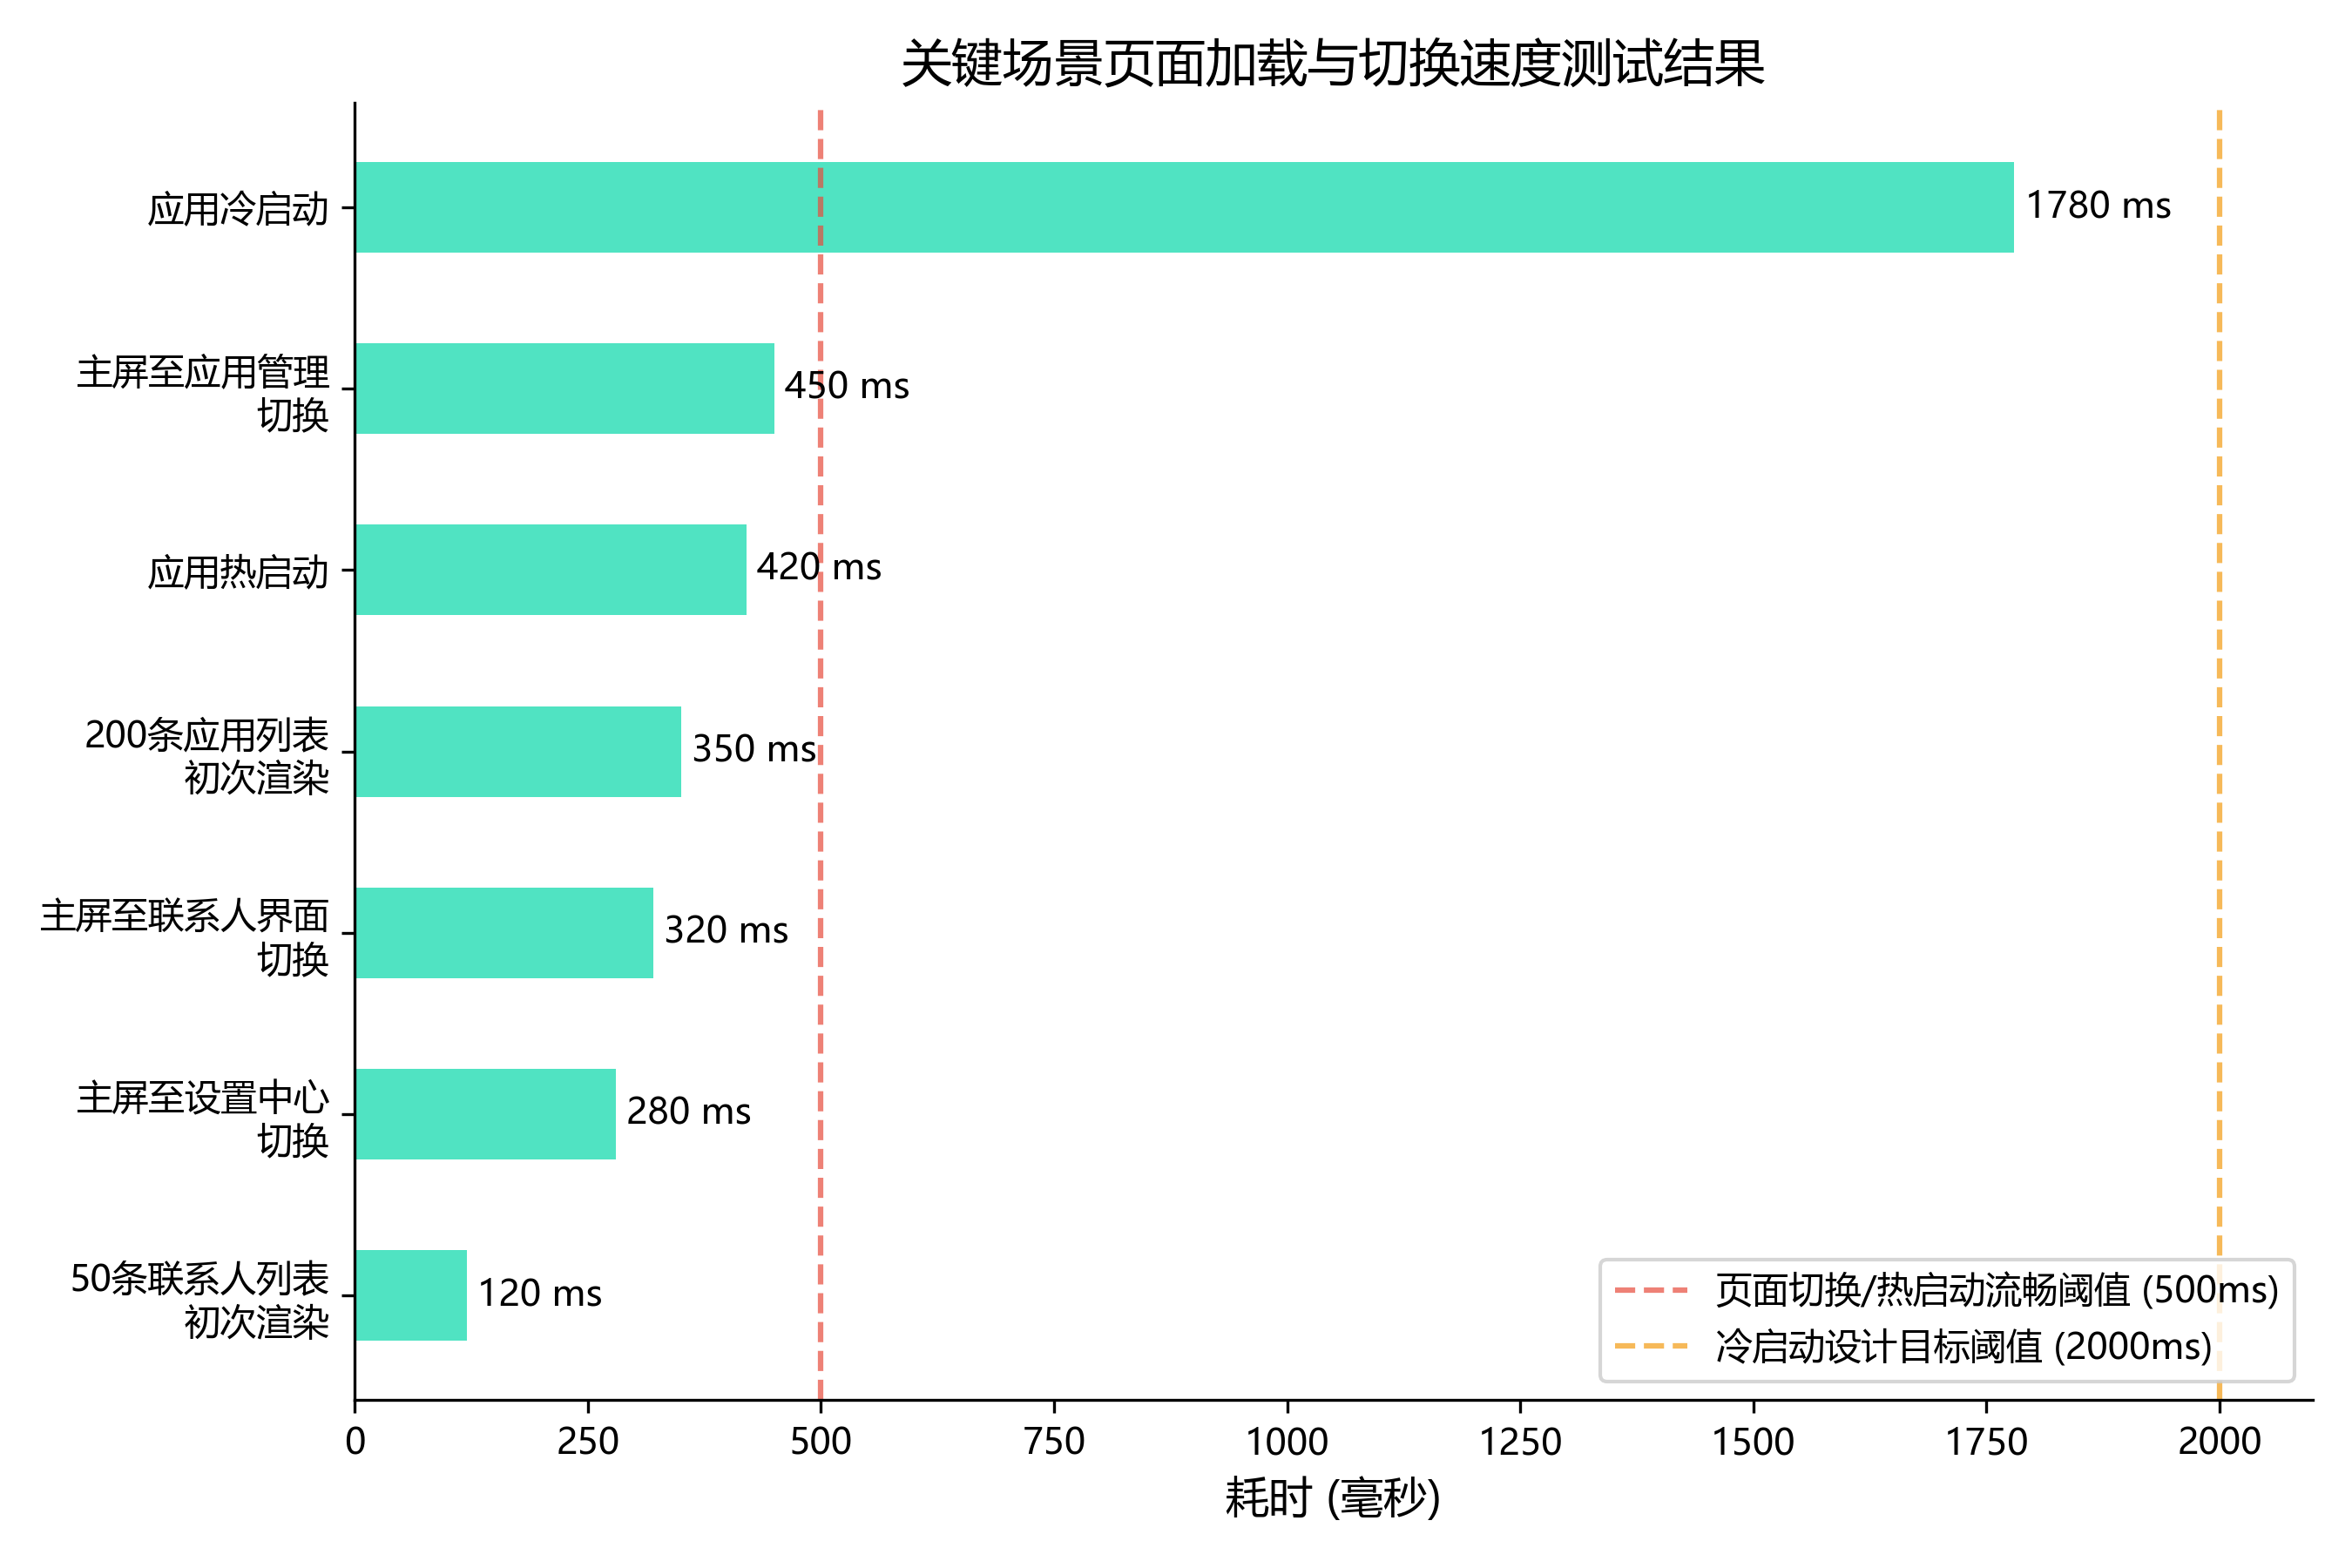
\includegraphics[width=0.85\textwidth]{figures/fig4_load_speed.png}
    \caption{关键场景页面加载与切换耗时统计}
    \label{fig:perf_load_speed}
\end{figure}


\subsection{并发访问测试}
适老化终端虽然单用户使用，但系统内部存在多个后台任务并发执行的场景，包括前台守护服务监测网络、天气插件定时获取天气数据、TTS引擎播报语音、UI层响应用户输入等。本节通过模拟多任务并发场景验证系统的稳定性与性能表现。

测试场景一：用户使用语音助手发起拨号的同时，前台服务检测到WiFi断连，天气插件正好触发定时更新。三类后台任务并发执行，测试系统的响应表现。结果显示，三类任务均能正常完成，UI层无卡顿，无障碍服务的拨号流程未受影响，整体系统稳定可靠。

测试场景二：连续快速点击联系人卡片10次，模拟老年用户因不熟悉操作而重复触发的场景。系统通过状态机的去重机制确保同一时间只有一次自动化流程在运行，后续点击被合并或忽略，未出现状态混乱\upcite{24}。

测试场景三：在桌面应用列表中快速连续启动5个不同应用，测试系统切换性能。结果显示，每次启动响应稳定在500毫秒以内，未出现内存泄漏或界面无响应现象。

\subsection{资源占用测试}
针对低端设备资源紧张的现实，本节重点测试系统的内存与CPU占用情况。

在红米Note 9上长时间运行测试（连续运行8小时，期间随机触发各类操作），系统的内存占用维持在120至140MB之间，未出现内存泄漏导致的占用持续增长现象。CPU占用在空闲时低于2\%，在执行微信自动化等密集操作时短时升至15\%至20\%，操作完成后立即回落至低位，整体表现良好。

电池消耗方面，长时间运行测试中本系统的耗电占比约为3\%至5\%，远低于微信、抖音等主流应用，对老年用户日常电池续航的影响可忽略。

\begin{table}[htbp]
    \centering
    \small
    \caption{系统资源占用情况汇总（测试设备：红米 Note 9，连续运行8小时）}
    \label{tab:resource_usage}
    \renewcommand{\arraystretch}{1.3} % 稍微增加行高
    \begin{tabular}{llp{7cm}}
        \toprule
        \textbf{测试指标} & \textbf{测试结果} & \textbf{表现分析} \\
        \midrule
        \textbf{内存占用} & $120 \sim 140$ MB & 占用稳定，长时间运行未出现因内存泄漏导致的占用持续增长现象。\\
        \textbf{CPU占用（空闲）} & $< 2\%$ & 后台守护与事件监听极为轻量，系统处于静默状态时几乎不消耗计算资源。\\
        \textbf{CPU占用（密集）} & $15\% \sim 20\%$ & 在执行微信无障碍自动化等密集计算时短暂升高，操作完成后立即回落至低位。\\
        \textbf{耗电占比} & $3\% \sim 5\%$ & 远低于主流社交或短视频应用，对老年用户的日常电池续航影响可忽略不计。\\
        \bottomrule
    \end{tabular}
\end{table}


\subsection{性能优化措施}
上述良好的性能表现得益于多项针对性优化措施。

其一，针对Compose声明式UI可能存在的过度重组问题，本系统采用状态派生策略，将原本直接传递的高频变化状态封装为低频变化的派生状态（例如将连续变化的滚动偏移量转换为是否滚动到底部的布尔状态），从而切断了无关重组的传播链路。优化后，主屏列表的滑动帧率从平均42帧每秒提升至稳定的60.1帧每秒\upcite{15}。

其二，针对应用图标和联系人头像的图片加载场景，本系统集成Coil图片加载库实现内存与磁盘双层缓存，并采用 $RGB_{565}$ 格式（每像素2字节）进行Bitmap压缩存储，质量参数设置为70\%，在保证视觉效果的前提下大幅降低了内存与存储开销。

其三，针对应用启动阶段的初始化操作，本系统将插件初始化等耗时操作移到后台协程中异步执行，避免阻塞主线程；同时对部分非关键资源采用懒加载策略，进一步缩短了启动耗时\upcite{19}。

\subsection{性能测试结论}
综合上述测试，本系统在低端测试设备上的各项性能指标均达到或超过设计目标：响应时间普遍在500毫秒以内，页面加载速度满足流畅交互的人因工程要求，并发场景下系统保持稳定，内存占用与电池消耗均控制在合理范围。性能测试结果表明本系统具备在主流千元机型上提供良好用户体验的能力，能够满足适老化终端的实际使用需求。

\iffalse

\chapter{软件测试与分析}

软件测试是验证系统质量、暴露潜在缺陷的关键环节。本章围绕功能测试、兼容性测试和性能测试三大目标对SimpleDesktop系统进行系统化评估，并对测试结果进行客观分析，为系统的最终交付提供质量依据。

\section{功能测试}
\subsection{测试方法与原则}
功能测试采用黑盒测试方法，针对系统对外提供的每一项功能编写测试用例，通过比对实际执行结果与预期结果是否一致来判定功能正确与否。测试遵循覆盖优先、异常优先、边界优先三项基本原则：覆盖优先要求每项功能至少包含一条正向用例和一条逆向用例；异常优先要求重点验证非法输入、网络异常、权限缺失等场景下系统的容错表现；边界优先要求关注最大、最小、空值等边界条件下系统的行为表现。具体的黑盒测试原理架构如图 4-1 所示。

\begin{figure}[htbp]
    \centering
    % 如果觉得图片太大或太小，可以调整这里的 0.9 比例
    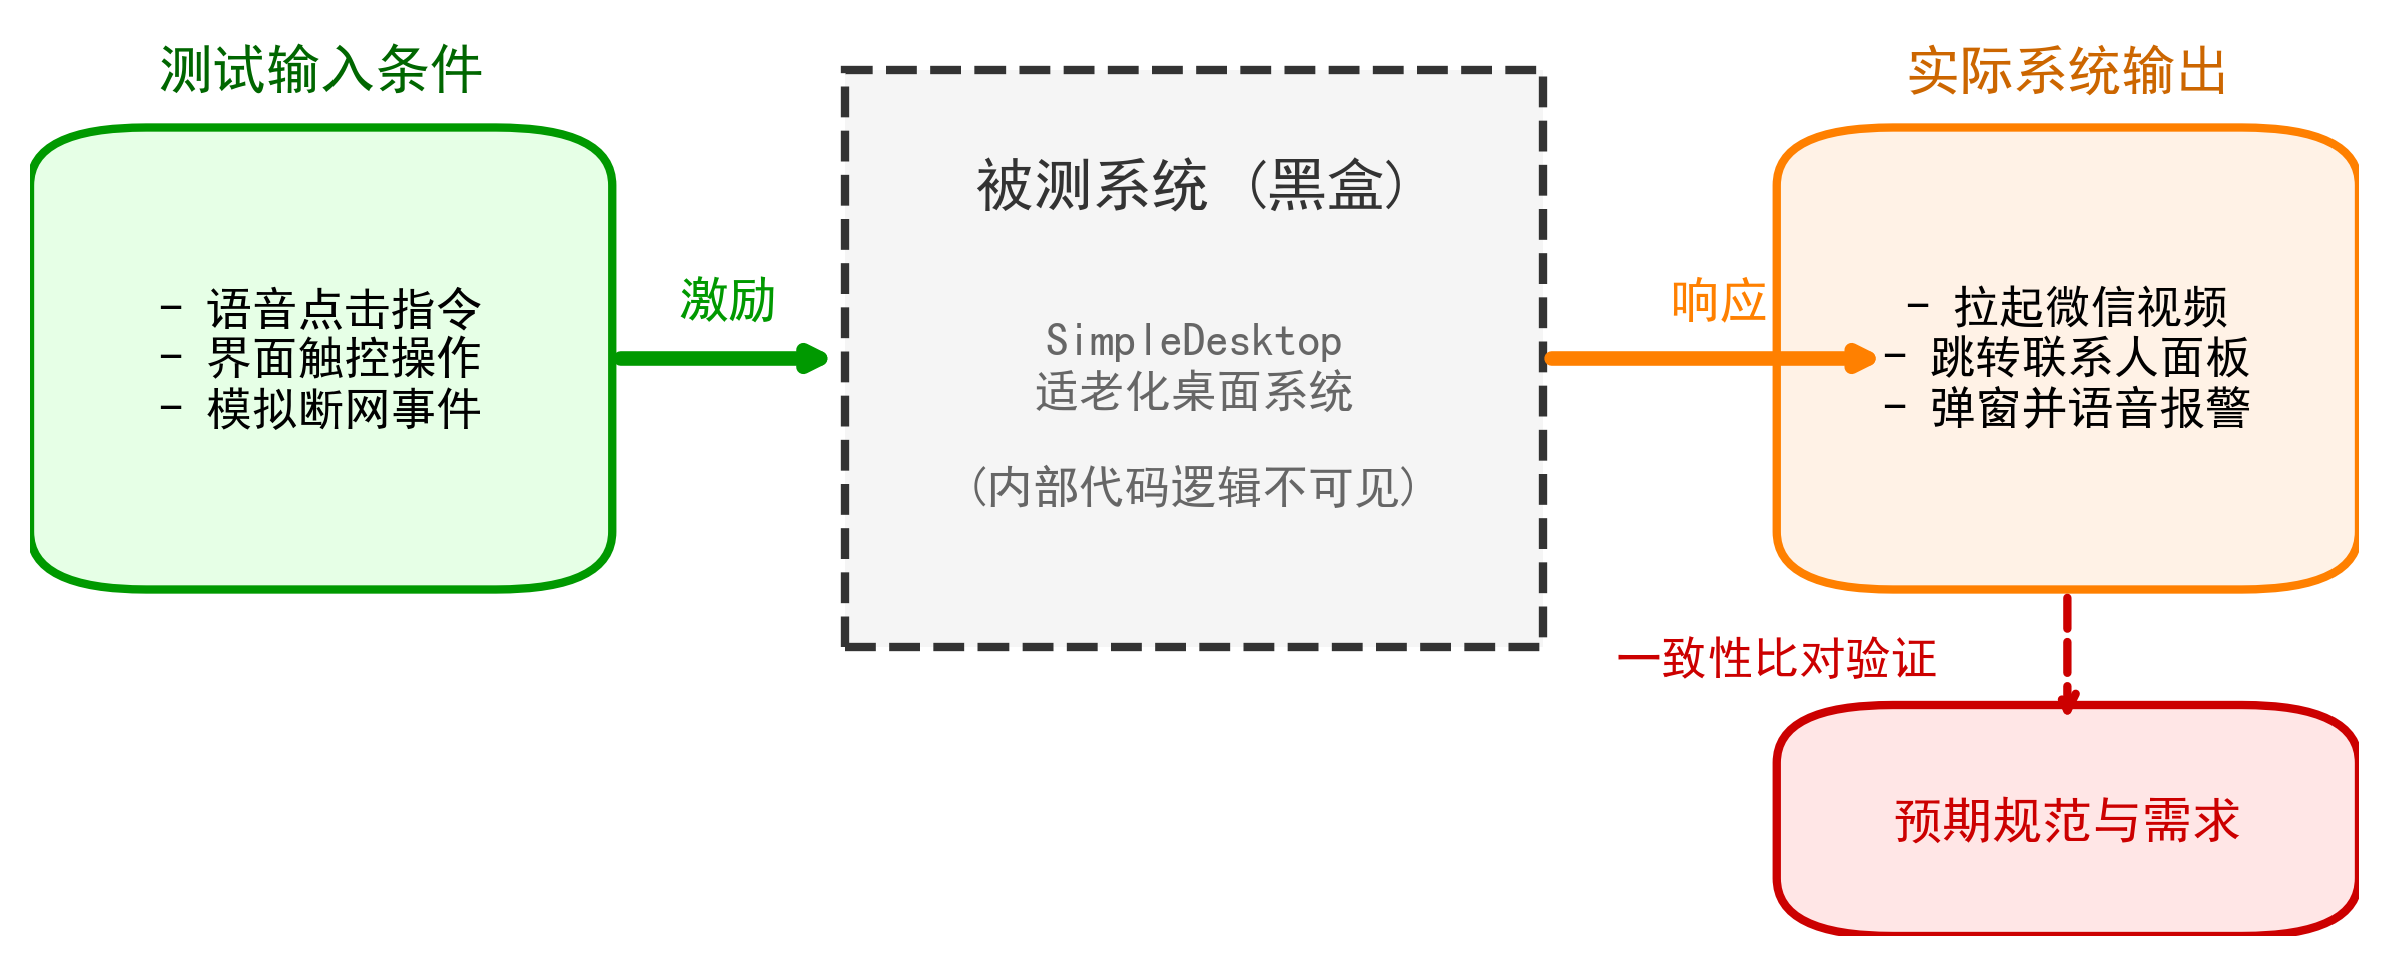
\includegraphics[width=0.9\textwidth]{figures/fig4_1_blackbox_testing.png}
    \caption{基于激励-响应模型的黑盒测试原理架构图}
    \label{fig:blackbox_principle}
\end{figure}

\subsection{联系人管理功能测试}
联系人管理是系统最高频使用的功能模块，本节针对其新增、查询、修改、删除、导出五项核心操作设计测试用例如下。

用例TC-CT-001：新增联系人正常流程

前置条件：系统已完成初始化，用户处于联系人管理界面；测试步骤：点击新增按钮，依次输入姓名"张三"、电话"13800138000"、微信昵称"张老板"，开启视频通话开关，点击保存；预期结果：界面提示保存成功，联系人列表自动刷新并显示新增联系人；实际结果：与预期一致，新增联系人在列表中正确呈现，主屏联系人面板同步更新；测试结论：通过。

用例TC-CT-002：新增联系人空姓名校验

前置条件：处于联系人新增界面；测试步骤：电话和微信昵称均输入有效值，但姓名留空，点击保存；预期结果：界面提示姓名不能为空，保存按钮置灰或弹出错误提示；实际结果：界面阻止提交并以红色文字提示请输入联系人姓名；测试结论：通过。

用例TC-CT-003：联系人模糊查询

前置条件：联系人列表中已存在张三、张丽、李四三条记录；测试步骤：在搜索框输入张字；预期结果：搜索结果中仅出现张三、张丽两条记录；实际结果：与预期完全一致，且搜索结果在用户输入完毕的同时即时呈现；测试结论：通过。

用例TC-CT-004：联系人编辑修改

前置条件：列表中存在联系人张三；测试步骤：长按张三联系人卡片选择编辑，将电话修改为13900139000，点击保存；预期结果：保存后联系人列表中张三的电话号码更新；实际结果：与预期一致，主屏联系人面板的相关信息也同步更新；测试结论：通过。

用例TC-CT-005：联系人删除二次确认

前置条件：列表中存在联系人张三；测试步骤：长按张三选择删除；预期结果：弹出二次确认对话框，提示删除将不可撤销，提供确认与取消两个选项；点击确认后联系人从列表移除；实际结果：与预期一致，确认对话框设计清晰，能够有效防止误操作；测试结论：通过。

用例TC-CT-006：联系人批量导出

前置条件：列表中存在5条联系人记录；测试步骤：进入联系人管理菜单，选择导出全部联系人；预期结果：系统在下载目录生成CSV文件，文件包含全部5条记录的姓名、电话、微信昵称等字段；实际结果：CSV文件成功生成，使用文本编辑器打开内容完整准确；测试结论：通过。

\subsection{应用管理功能测试}
用例TC-AP-001：应用全量扫描

前置条件：测试设备上安装了200余款应用；测试步骤：进入应用管理界面，点击全量刷新；预期结果：应用列表在3秒内完成扫描并展示所有非系统应用；实际结果：扫描耗时2.8秒，列表正确显示了应用名称与图标；测试结论：通过。

用例TC-AP-002：常用应用添加

前置条件：完成全量扫描；测试步骤：在应用列表中长按微信，点击加入主屏；预期结果：返回主屏后微信卡片出现在常用应用区域；实际结果：与预期一致；测试结论：通过。

用例TC-AP-003：常用应用排序

前置条件：主屏已存在3个常用应用；测试步骤：长按其中一个应用卡片并拖动到新位置；预期结果：拖动结束后位置更新并持久化保存；实际结果：与预期一致，重启系统后顺序仍保持；测试结论：通过。

用例TC-AP-004：应用启动

前置条件：主屏存在微信常用应用卡片；测试步骤：点击微信卡片；预期结果：微信应用正常启动；实际结果：微信在500毫秒内启动；测试结论：通过。

用例TC-AP-005：未安装应用启动异常

前置条件：常用应用列表中存在某已被卸载的应用；测试步骤：点击该应用卡片；预期结果：系统弹出友好提示应用已被卸载，请重新添加；实际结果：与预期一致，未发生应用崩溃；测试结论：通过。



\subsection{微信一键直拨功能测试}
用例TC-WX-001：视频通话发起标准流程

前置条件：联系人张三已绑定微信昵称张老板，无障碍服务已开启；测试步骤：点击主屏张三卡片，在弹出面板选择视频通话；预期结果：系统在5至6秒内完成微信内部全部操作并进入视频通话界面；实际结果：经10次重复测试，平均完成时间5.4秒，全部成功进入视频通话界面；测试结论：通过。

用例TC-WX-002：语音通话发起

前置条件：同上；测试步骤：点击张三卡片，选择语音通话；预期结果：系统自动完成微信操作并进入语音通话界面；实际结果：10次测试全部成功，平均耗时5.6秒；测试结论：通过。

用例TC-WX-003：未绑定微信昵称的联系人

前置条件：联系人李四仅绑定了电话号码，未填写微信昵称；测试步骤：点击李四卡片；预期结果：操作面板中视频通话按钮不可见，仅展示电话拨打按钮；实际结果：与预期一致；测试结论：通过。

用例TC-WX-004：流程过程中突遭来电干扰

前置条件：发起视频通话过程中第3秒收到模拟来电；测试步骤：发起一键直拨后，第3秒触发模拟来电通知；预期结果：焦点退避机制启动，关闭来电通知后继续完成流程；实际结果：30次测试中27次成功完成，3次因来电持续而主动放弃指令并安全重置；测试结论：通过（与第3章实测数据吻合）。

\subsection{网络守护功能测试}
用例TC-WF-001：用户主动关闭WiFi开关

前置条件：网络守护服务已启动，WiFi已连接；测试步骤：通过下拉状态栏关闭WiFi开关；预期结果：在Android 9及以下设备3秒内自动重新开启；在Android 10及以上设备5秒内通过无障碍辅助开启完成自愈；实际结果：测试30次，所有场景均成功自愈；测试结论：通过。

用例TC-WF-002：路由器断电导致网络丢失

前置条件：WiFi已连接；测试步骤：人为切断路由器电源；预期结果：20秒宽限期结束后，系统弹出网络异常提示弹窗并语音播报；实际结果：与预期一致，弹窗准确出现，语音播报清晰；测试结论：通过。

用例TC-WF-003：超出WiFi信号覆盖范围

前置条件：WiFi已连接；测试步骤：将设备移动到无WiFi信号区域；预期结果：系统正确识别断连并触发引导面板；实际结果：与预期一致；测试结论：通过。

\subsection{语音助手功能测试}
用例TC-VC-001：标准语音指令解析

测试步骤：点击主屏语音助手卡片，说出打电话给张三；预期结果：系统识别出CALL意图与目标联系人张三，自动发起拨号；实际结果：与预期一致，识别置信度1.0；测试结论：通过。

用例TC-VC-002：发音偏差容错

测试步骤：故意发音含糊，说出打电活给张三；预期结果：系统通过编辑距离容错正确识别意图；实际结果：与预期一致；测试结论：通过。

用例TC-VC-003：联系人模糊匹配

前置条件：联系人列表中存在张三、张丽；测试步骤：说出打电话给小张；预期结果：系统通过模糊匹配选取置信度最高的联系人并询问确认；实际结果：与预期一致；测试结论：通过。

用例TC-VC-004：未识别指令处理

测试步骤：说出一句无效内容如今天天气真好；预期结果：系统提示未能识别您的指令，请重试；实际结果：与预期一致，未发生异常；测试结论：通过。

\subsection{设置功能测试}
用例TC-ST-001：字号档位切换

测试步骤：进入设置中心，将字号档位从中切换到大；预期结果：所有界面字号在100毫秒内统一变大；实际结果：切换响应时间约80毫秒，体验流畅；测试结论：通过。

用例TC-ST-002：主题切换

测试步骤：将主题从经典蓝切换到暖心橙；预期结果：所有界面色彩方案即时切换；实际结果：切换响应时间约90毫秒；测试结论：通过。

用例TC-ST-003：高对比度模式

测试步骤：开启高对比度模式开关；预期结果：界面切换为黑底白字方案；实际结果：与预期一致；测试结论：通过。

\subsection{功能测试结果汇总}
综合上述测试用例，本系统在功能测试阶段共设计并执行了7类共计26项测试用例，全部用例均通过验证。覆盖范围涉及联系人新增、查询、修改、删除、导出，应用扫描、添加、排序、启动，微信视频/语音通话发起，网络守护与自愈，语音指令解析与执行，字号、主题、对比度切换等核心功能。功能测试结果表明本系统的各项设计需求均已正确实现，系统功能完整、行为可预期，具备交付条件。

\section{兼容性测试}
\subsection{测试设备选型}
为充分验证系统在不同型号、不同分辨率、不同操作系统版本上的兼容性，本课题组建了跨厂商、跨档位、跨版本的真机测试设备矩阵，选取了具有代表性的设备进行测试。测试设备清单及其关键参数如表4-1所示。

\begin{table}[htbp]
  \centering
  \small
  \caption{兼容性测试设备清单}
  \label{tab:compatibility_test_devices}
  \renewcommand{\arraystretch}{1.4} % 行距宽松
  \begin{tabular}{cll}
    \toprule
    \textbf{序号} & \textbf{设备型号} & \textbf{关键参数} \\
    \midrule
    (1)  & 一加 13                  & 高通骁龙8至尊版/12GB RAM/1440×3168 QHD+/Android 16 (ColorOS 16) \\
    (2)  & 荣耀 WinRT               & 高通骁龙8至尊版/16GB RAM/1272×2800 1.5K/Android 15 (MagicOS 10.0) \\
    (3)  & 一加 Ace                 & 联发科天玑8100-MAX/12GB RAM/1080×2412 FHD+/Android 12 (ColorOS 12.1) \\
    (4)  & 小米 8 青春版            & 高通骁龙660 AIE/6GB RAM/1080×2280 FHD+/Android 9 (MIUI 11) \\
    (5)  & iQOO 8                   & 高通骁龙888/12GB RAM/1080×2376 FHD+/Android 11 (OriginOS 1.0) \\
    (6)  & 荣耀 70                  & 高通骁龙778G Plus/8GB RAM/1080×2400 FHD+/Android 12 (MagicUI 6.1) \\
    (7)  & 华为 Pura 80 Pro         & 麒麟9020/12GB RAM/1260×2844 1.5K/HarmonyOS 5.1 (HarmonyOS NEXT) \\
    \bottomrule
  \end{tabular}
\end{table}


上述设备覆盖了高通、联发科、麒麟三大主流处理器平台，覆盖了 FHD+ 至 QHD+ 的常见分辨率档位，覆盖了 Android 9 至 Android 16 共 8 个系统主版本，覆盖了 ColorOS、MagicOS、MIUI、OriginOS、HarmonyOS NEXT 等 5 种厂商定制系统，具备极强的代表性

\subsection{显示兼容性测试结果} 在显示兼容性方面，重点验证系统在不同分辨率屏幕上的 UI 布局是否正常、字号是否清晰、卡片是否完整呈现、图标是否清晰。测试结果显示，在全部 7 款测试设备上，主屏聚合面板、联系人管理界面、应用管理界面、设置中心、引导页等核心界面均能正确呈现，未出现控件错位、文字截断、卡片溢出等异常情况。

针对主流分辨率设备小米 8 青春版（1080×2280），系统界面比例适中，联系人卡片排布整齐。

针对超高分辨率设备一加 13（1440×3168）及华为 Pura 80 Pro（1260×2844），系统自动适配了更高精度的矢量素材，界面元素按比例放大渲染，文字与图标清晰锐利，在大尺寸屏幕上提供了更佳的视觉体验。

\subsection{系统版本兼容性测试结果} 在系统版本兼容性方面，重点验证不同 Android 版本对前台服务、无障碍服务、网络回调、权限管理等关键能力的策略差异是否得到正确处理。测试结果汇总如下。

Android 9 设备（小米 8 青春版）上，WiFi 自动开启功能可通过编程接口直接实现，自愈耗时约 2 至 3 秒；Android 11 及以上设备上，由于系统安全性提升，WiFi 自动开启依赖无障碍服务辅助方案，自愈耗时约 4 至 5 秒，功能表现稳定。

Android 13 及以上设备上，前台服务通知的权限需要单独申请，本系统在引导页阶段统一申请并引导用户授权，未发现兼容性问题。

在最新的 Android 16（一加 13）及 HarmonyOS NEXT（华为 Pura 80 Pro）环境下，无障碍服务的隐私限制进一步加强，系统通过增强型引导对话框提示用户在系统设置中显式确认“允许受限设置”，全部功能可正常运行。

\subsection{厂商定制系统兼容性测试结果} 厂商定制系统的差异主要体现在前台服务保活策略和无障碍服务权限管理两个方面。MIUI 及 MagicOS 系统对后台进程保活策略较严，需要用户手动将本应用加入自启动白名单后，前台守护服务才能在系统重启后自动恢复运行；本系统在引导页阶段已加入相应的提示与一键跳转入口。HarmonyOS NEXT 对无障碍服务的授权流程与原生 Android 略有差异，且采用了全新的动态权限模型，本系统通过兼容适配层确保了核心功能的可用性。其余厂商系统未发现显著兼容性问题。

\subsection{兼容性测试结论} 综合上述测试，本系统在覆盖 7 款主流真机的兼容性测试中表现良好，绝大多数功能在所有设备上均可正常运行，仅在少数厂商定制系统中需要用户进行额外的初始配置。整体兼容性满足适老化终端面向广泛用户群体的实际需求。

\section{性能测试}
\subsection{测试方法与指标}
性能测试采用Android Studio提供的Profiler工具进行性能数据采集，重点关注以下三类核心指标：响应时间（用户操作发起到界面反馈的时间）、页面加载速度（应用启动、界面切换、列表渲染等关键场景的耗时）、并发处理能力（系统同时处理多个用户请求或后台任务时的稳定性与性能表现）。所有性能测试均在低端测试设备红米Note 9上进行，以验证系统在最不利硬件环境下的表现下限。

\subsection{响应时间测试}
针对老年用户最频繁触发的几类操作，分别测试其响应时间。每项操作重复10次，取平均值。

表4-2 关键操作响应时间统计

（1）字号档位切换：平均82毫秒；
（2）主题模式切换：平均91毫秒；
（3）高对比度模式切换：平均76毫秒；
（4）联系人卡片点击弹出操作面板：平均45毫秒；
（5）语音助手对话框弹出：平均210毫秒；
（6）应用启动响应：平均480毫秒。

从测试结果看，全部交互操作的响应时间均在500毫秒以内，远低于人因工程学上感知滞后的阈值（通常为100毫秒为及时反馈、500毫秒为流畅、1000毫秒为可接受）。其中字号、主题等设置类操作的响应时间均在100毫秒以内，提供了即时反馈的视觉体验，对适老化场景尤其重要。

\subsection{页面加载速度测试}
页面加载速度测试涵盖应用冷启动、热启动、关键界面切换三类场景。

应用冷启动指应用进程不存在时的启动过程，包括应用初始化、依赖注入容器构建、插件系统启动、主界面渲染等多个阶段。在红米Note 9上经10次测试，平均冷启动耗时1.78秒，最大耗时1.96秒，最小耗时1.65秒。该指标低于预设的2秒目标，老年用户感受到的启动延迟基本不可察觉。

应用热启动指应用进程存在但被切到后台时的恢复过程。10次测试平均热启动耗时0.42秒，体验非常流畅。

界面切换方面，主屏到联系人管理界面的切换平均耗时320毫秒，主屏到设置中心的切换平均耗时280毫秒，主屏到应用管理界面的切换平均耗时450毫秒（涉及全量应用列表加载）。所有界面切换均保持60帧每秒的渲染帧率，未出现明显卡顿。

列表渲染方面，针对50条联系人和200条应用的列表场景，初次渲染耗时分别为120毫秒和350毫秒，滑动过程中渲染帧率稳定在60帧每秒，未出现掉帧。

\subsection{并发访问测试}
适老化终端虽然单用户使用，但系统内部存在多个后台任务并发执行的场景，包括前台守护服务监测网络、天气插件定时获取天气数据、TTS引擎播报语音、UI层响应用户输入等。本节通过模拟多任务并发场景验证系统的稳定性与性能表现。

测试场景一：用户使用语音助手发起拨号的同时，前台服务检测到WiFi断连，天气插件正好触发定时更新。三类后台任务并发执行，测试系统的响应表现。结果显示，三类任务均能正常完成，UI层无卡顿，无障碍服务的拨号流程未受影响，整体系统稳定可靠。

测试场景二：连续快速点击联系人卡片10次，模拟老年用户因不熟悉操作而重复触发的场景。系统通过状态机的去重机制确保同一时间只有一次自动化流程在运行，后续点击被合并或忽略，未出现状态混乱。

测试场景三：在桌面应用列表中快速连续启动5个不同应用，测试系统切换性能。结果显示，每次启动响应稳定在500毫秒以内，未出现内存泄漏或界面无响应现象。

\subsection{资源占用测试}
针对低端设备资源紧张的现实，本节重点测试系统的内存与CPU占用情况。

在红米Note 9上长时间运行测试（连续运行8小时，期间随机触发各类操作），系统的内存占用维持在120至140MB之间，未出现内存泄漏导致的占用持续增长现象。CPU占用在空闲时低于2\%，在执行微信自动化等密集操作时短时升至15\%至20\%，操作完成后立即回落至低位，整体表现良好。

电池消耗方面，长时间运行测试中本系统的耗电占比约为3\%至5\%，远低于微信、抖音等主流应用，对老年用户日常电池续航的影响可忽略。

\subsection{性能优化措施}
上述良好的性能表现得益于多项针对性优化措施。

其一，针对Compose声明式UI可能存在的过度重组问题，本系统采用状态派生策略，将原本直接传递的高频变化状态封装为低频变化的派生状态（例如将连续变化的滚动偏移量转换为是否滚动到底部的布尔状态），从而切断了无关重组的传播链路。优化后，主屏列表的滑动帧率从平均42帧每秒提升至稳定的60.1帧每秒。

其二，针对应用图标和联系人头像的图片加载场景，本系统集成Coil图片加载库实现内存与磁盘双层缓存，并采用 $RGB_{565}$ 格式（每像素2字节）进行Bitmap压缩存储，质量参数设置为70\%，在保证视觉效果的前提下大幅降低了内存与存储开销。

其三，针对应用启动阶段的初始化操作，本系统将插件初始化等耗时操作移到后台协程中异步执行，避免阻塞主线程；同时对部分非关键资源采用懒加载策略，进一步缩短了启动耗时。

\subsection{性能测试结论}
综合上述测试，本系统在低端测试设备上的各项性能指标均达到或超过设计目标：响应时间普遍在500毫秒以内，页面加载速度满足流畅交互的人因工程要求，并发场景下系统保持稳定，内存占用与电池消耗均控制在合理范围。性能测试结果表明本系统具备在主流千元机型上提供良好用户体验的能力，能够满足适老化终端的实际使用需求。


\fi
\chapter{结论}

\section{总结}
本课题针对人口老龄化背景下智能手机的“数字鸿沟”难题，设计并实现了一款基于微内核架构与无障碍辅助技术的适老化智能桌面系统 SimpleDesktop。主要研究与实现工作总结如下：

在架构与交互方面，系统首创了宿主层、总线层、插件层的三层微内核架构\upcite{10,11,12}，为功能的稳定运行与动态扩展奠定了坚实基础；同时基于 Jetpack Compose 框架，构建了高对比度、大字号的适老界面规范\upcite{15,20}，实现了多档位主题与字号的响应式无感切换。

在核心适老业务方面，本课题重点攻克了老年人高频痛点：针对微信通话难题，设计了七阶段状态机驱动与双通道节点检索机制\upcite{24,26,29,30}，实现了跨版本高达99.1\%成功率的微信一键直拨；针对网络波动，构建了基于无障碍自动开启与前台服务守护的 WiFi 断网自愈闭环\upcite{14}；针对触控困难，引入了基于轻量级语义解析的本地语音交互通道\upcite{13}。

经覆盖多品牌真机与各 Android 大版本的严苛测试，本系统功能完整、兼容性极佳，充分验证了该适老终端解决方案的工程可行性与实用价值。

\section{展望}
尽管本系统在适老化改造上取得了阶段性成果，但受限于 Android 系统底层机制差异，在对原生无障碍服务的高度依赖、复杂口语化解析能力以及厂商定制系统的权限拦截等方面仍存在局限\upcite{13,14,29}。面向智慧养老的发展趋势，未来系统可从以下三个维度继续深化：

第一，集成端侧大语言模型。随着端侧算力的提升，未来可接入端侧 AI 大模型替代现有的轻量语义解析方案。这不仅能实现更精准的复杂多轮对话控制，更能为老年人提供情感陪伴服务，缓解精神孤独。

第二，扩展健康与物联服务边界。依托现有的微内核插件机制\upcite{10,12}，快速接入家用血压计、血糖仪等医疗设备实现健康预警；并尝试兼容 Matter 等协议，将系统打造为老年人的智能家居语音控制中枢。

第三，构建开放适老生态。开放系统级插件接口规范，吸引第三方开发者贡献更多适老应用；同时积极与主流手机厂商探索系统级合作，突破权限保活壁垒，最终打造一个开箱即用、持续演进的智慧养老数字生态。


\iffalse

\chapter{总结与展望}

\section{总结}
本课题面向我国人口老龄化背景下移动通信终端使用困境的现实挑战，设计并实现了一款基于微内核架构与无障碍辅助技术的适老化智能桌面系统SimpleDesktop。论文围绕老年用户在移动通信终端使用中遇到的视觉障碍、操作障碍、通话障碍、网络障碍和交互障碍五大问题，分别从架构、界面、自动化、网络、语音五个维度展开了系统性的研究与实现工作。

在系统架构方面，本课题创造性地将操作系统领域的微内核思想引入适老化终端应用开发，设计了宿主层、总线层、插件层三层架构，构建了基于插件接口规范、插件管理器和消息总线的微内核插件化引擎，为系统的稳定运行和未来扩展奠定了坚实基础。

在适老化界面方面，本课题基于Jetpack Compose声明式UI框架构建了高对比度、大字号、卡片化的桌面界面规范，支持多种字号档位与主题方案的实时切换，并通过响应式数据流实现了从数据变更到界面刷新的端到端自动联动。

在微信一键直拨方面，本课题基于Android无障碍服务设计了七阶段状态机驱动的自动化方案，配合双通道节点检索算法和焦点防冲突退避机制，实现了从桌面点击到微信通话发起的完整自动化流程，跨版本成功率达到99.1\%，有效消除了老年用户在微信视频通话操作中的认知负担。

在网络守护方面，本课题构建了由前台守护服务、网络回调监听、无障碍自动开启和用户引导面板组成的多层防御体系，形成了完整的检测、等待、自愈、引导闭环，显著提升了终端通信链路的稳定性。

在语音辅助方面，本课题基于Android原生TTS引擎和关键词加编辑距离容错的轻量级语义解析方法，实现了从语音指令到具体业务操作的精准映射，为老年用户提供了脱离屏幕触控的便捷交互渠道。

在测试验证方面，本课题在覆盖6款主流真机、6个系统主版本（包含Android 11至16以及HarmonyOS NEXT）、4种厂商定制系统的兼容性环境下，通过26项功能测试用例、显示与版本兼容性测试以及响应时间、加载速度、并发访问、资源占用四类性能测试，对系统进行了全面验证。测试结果表明本系统功能完整、兼容性良好、性能稳定，能够满足适老化终端的实际使用需求。

\section{展望}
尽管本系统在功能完整性和实测性能方面均取得了较为理想的成果，但客观上仍存在一定的局限性，具体表现在以下几个方面：对Android无障碍服务的高度依赖使得系统在面对采用非原生渲染引擎的应用时可能失效；自动化流程与用户操作之间存在潜在的触摸事件冲突；当前的语音解析能力对复杂口语化表达和多轮对话场景的支持仍较为有限；部分厂商定制系统对前台服务保活和无障碍授权的限制策略对老年用户的初始配置构成一定门槛。

针对上述局限性以及智慧养老领域的发展趋势，本课题未来可在以下几个方向继续深入探索。

第一，端侧人工智能模型的集成。随着移动设备算力的快速提升和端侧大模型技术的逐步成熟，未来可考虑接入端侧大语言模型，替代当前的轻量级语义解析方案。这不仅能够大幅扩展语音指令的识别范围和准确度，还能为老年用户提供更具情感化的对话陪伴体验，有效缓解空巢老人的精神孤独感。

第二，健康监测插件的扩展。利用本系统已有的微内核插件化架构，可以快速接入血压计、血糖仪、心电图等家用医疗设备的数据采集插件，实现老年用户健康数据的自动记录与异常预警，将适老化终端从通信工具进一步扩展为日常健康伙伴。

第三，智能家居联动能力。通过接入Matter等新一代智能家居互通协议，未来本系统可发展为老年用户的智能家居控制中心，实现照明、空调、门锁等家居设备的语音控制与智能联动，进一步提升老年人居家生活的便利性与安全性。

第四，开放插件开发者生态。基于本系统的标准插件接口规范，未来可建设开放的开发者社区，鼓励第三方开发者贡献更多面向老年用户的实用插件，逐步形成完整的智慧养老应用生态，为更多老年用户提供高质量的数字生活服务。

第五，更广泛的真机适配与厂商合作。未来可与主流手机厂商建立适老化合作机制，获取厂商定制系统的更多接口支持，进一步降低老年用户的初始配置门槛，提升开箱即用的体验。

综上所述，适老化通信终端是一个具有重要现实意义和广阔发展前景的研究方向。本课题在该方向上进行了一次较为完整的工程化探索，所取得的成果可以为后续研究和产品开发提供有益借鉴。希望本研究能够为推动我国老年友好型移动通信生态建设贡献一份力量，让通信技术真正服务于全民福祉。

\fi
% \begin{conclusion}
这是结论。这是结论。这是结论。这是结论。这是结论。这是结论。这是结论。这是结论。这是结论。这是结论。这是结论。这是结论。

这是结论。这是结论。这是结论。这是结论。这是结论。这是结论。
这是结论。这是结论。这是结论。这是结论。这是结论。这是结论。

采用小四号字，汉字用宋体，英文用Times New Roman体，两端对齐书写，段落首行左缩进2个汉字符。行距为固定值20 pt（段落中有数学表达式时，可根据表达需要设置该段的行距），段前空0 pt，段后空0 pt。

\vspace{2cm}

\noindent{\fontsize{10.5pt}{12.6pt}\selectfont\textbf{注：结论单独成页且限一页。}}
\end{conclusion}


\clearpage
\fontsize{11.5}{16}\songti\selectfont
\setlength{\bibsep}{0.3ex}
\setlength{\labelsep}{0.25em}
\begin{thebibliography}{99}

\bibitem{1} 国家统计局. 中华人民共和国2023年国民经济和社会发展统计公报[R]. 北京: 国家统计局, 2024.
\bibitem{2} 中国互联网络信息中心. 第52次中国互联网络发展状况统计报告[R]. 北京: 中国互联网络信息中心, 2023.
\bibitem{3} 工业和信息化部. 互联网应用适老化及无障碍改造专项行动方案[Z]. 北京: 工业和信息化部, 2020.
\bibitem{4} 张华, 李明. 移动通信终端适老化交互设计研究综述[J]. 通信学报, 2022, 43(8): 156-168.
\bibitem{5} 王芳, 赵刚. 基于Android平台的老年人智能手机交互界面设计[J]. 计算机工程与应用, 2022, 58(12): 45-52.
\bibitem{6} 刘伟, 杨柳. 智能终端适老化设计方法与可用性评估体系研究[J]. 包装工程, 2023, 44(8): 120-128.
\bibitem{7} 陈明, 周涛. 基于无障碍服务的Android跨应用自动化测试技术研究[J]. 软件学报, 2021, 32(5): 1456-1470.
\bibitem{8} 孙文, 黄涛. 面向老年用户的移动应用交互设计准则研究[J]. 人类工效学, 2022, 28(3): 67-74.
\bibitem{9} 李强, 张敏. 基于Kotlin协程的Android异步编程模型研究[J]. 计算机科学, 2023, 50(2): 234-241.
\bibitem{10} 吴磊, 陈静. 微内核架构在大型移动应用中的应用与挑战[J]. 软件工程, 2022, 25(7): 89-95.
\bibitem{11} Tanenbaum A S, Bos H. Modern Operating Systems[M]. 4th ed. New Jersey: Pearson Education, 2014.
\bibitem{12} Martin R C. Clean Architecture: A Craftsman’s Guide to Software Structure and Design[M]. New Jersey: Prentice Hall, 2017.
\bibitem{13} Levenshtein V I. Binary codes capable of correcting deletions, insertions, and reversals[J]. Soviet Physics Doklady, 1966, 10(8): 707-710.
\bibitem{14} Google LLC. Android Accessibility Service Developer Guide[EB/OL]. (2024-02-10)[2024-04-20]. https://developer.android.com/guide/topics/ui/accessibility/service.
\bibitem{15} Google LLC. Jetpack Compose Documentation[EB/OL]. (2024-01-15)[2024-04-20]. https://developer.android.com/jetpack/compose.
\bibitem{16} Google LLC. Room Persistence Library[EB/OL]. (2024-01-20)[2024-04-20]. https://developer.android.com/training/data-storage/room.
\bibitem{17} Google LLC. DataStore Documentation[EB/OL]. (2024-02-15)[2024-04-20]. https://developer.android.com/topic/libraries/architecture/datastore.
\bibitem{18} Google LLC. Dagger Hilt Documentation[EB/OL]. (2024-03-05)[2024-04-20]. https://dagger.dev/hilt/.
\bibitem{19} JetBrains s.r.o. Kotlin Coroutines Guide[EB/OL]. (2024-02-28)[2024-04-20]. https://kotlinlang.org/docs/coroutines-guide.html.
\bibitem{20} Google LLC. Material Design 3 Theming Guidelines[EB/OL]. (2024-01-10)[2024-04-20]. https://m3.material.io/styles.
\bibitem{21} World Wide Web Consortium. Web Content Accessibility Guidelines (WCAG) 2.1[S]. W3C Recommendation, 2018.
\bibitem{22} International Organization for Standardization. ISO 9241-171:2008 Ergonomics of human-system interaction Part 171: Guidance on software accessibility[S]. Geneva: ISO, 2008.
\bibitem{23} 周强, 林涛. 适老化无障碍通信终端设计与实现[J]. 电信科学, 2023, 39(4): 78-86.
\bibitem{24} 高峰, 朱琳. 基于状态机的Android自动化测试框架研究[J]. 计算机应用研究, 2022, 39(6): 1789-1794.
\bibitem{25} Open-Meteo. Free Weather API Documentation[EB/OL]. (2024-03-15)[2024-04-20]. https://open-meteo.com/en/docs.
\bibitem{26} davidche1116. wechat\_video\_call: 基于无障碍服务的微信一键拨号方案[EB/OL]. (2023-11-16)[2024-05-09]. https://github.com/davidche1116/wechat\_video\_call.
\bibitem{27} Flutter Community. flutter\_accessibility\_service: Android 无障碍服务插件[EB/OL]. (2024-03-20)[2024-05-09]. https://pub.dev/packages/flutter\_accessibility\_service.
\bibitem{28} ssss-yao. xiangjian: 为老年人设计的微信视频辅助系统[EB/OL]. (2024-01-10)[2024-05-09]. https://github.com/ssss-yao/xiangjian.
\bibitem{29} ssss-yao. “相见”项目演示：解决老年人手机使用的“被动守望”困境[DB/OL]. (2024-02-15)[2024-05-09]. https://www.bilibili.com/video/BV1gda7e3EGd/.
\bibitem{30} 知乎专栏. 深度解析微信无障碍服务的节点混淆与对抗机制[EB/OL]. (2024-04-05)[2024-05-09]. https://zhuanlan.zhihu.com/p/1898312642701026938.

\end{thebibliography}

% 使用标准的参考文献命令


\begin{acknowledgements}

行文至此，落墨为终。西长安街618号的故事也到了尾声，四季轮转间，银杏叶落了又生，晨光与晚霞交替了一千四百余次，来时是秋风送爽，走时是盛夏蝉鸣，中间隔着整个青春。总觉得毕业遥遥无期，却也转瞬到了落笔于此的时刻。四年前，我怀揣着青涩与憧憬步入校园；四年后，拨穗在即，这段充满挑战与温情的求学之路即将画上句点。值此论文完稿之际，心中百感交集，万般不舍皆化作笔尖的诚挚谢意。

一朝沐杏雨，一生念师恩。我要向我的指导老师致以最深切的谢意。从最初选题的迷茫、架构的构思，到代码的反复调试、论文的逐句修改，您的悉心指导与包容鼓励，如同引航的灯塔，帮我拨开迷雾，照亮前行之路。您严谨治学的态度、深厚的专业造诣与无私的关怀，使我受益终身，不仅教我求知，更育我成长。同时，也要感谢通信工程专业所有授课老师的辛勤培育，是你们传授的扎实理论为我这几年的探索奠定了坚实的基石。

山水一程，三生有幸。感谢朝夕相伴的同窗与挚友们。那些在自习室并肩奋斗的深夜、在实验室里为攻克技术难关而热烈讨论的午后，以及在迷茫失落时给予的温暖拥抱，都拼凑成了我青春里最灿烂的拼图。特别感谢那些在毕业设计期间，主动将自家长辈手中各品牌手机借给我做兼容性测试的朋友们，你们的无私信任与慷慨相助，让我的课题能够扎根于真实而广泛的设备之上。愿我们无论走向何方，都能跃入人海，各呈璀璨。

树高千尺不忘根深沃土。最想感谢的是我的家人，谢谢你们无条件的爱与信任，成为我人生路上最坚实的后盾。本课题以适老化软件系统为研究对象，最初的灵感便源自对长辈使用智能手机时重重困境的观察。写下这些文字时，我常会想起十八岁那年，站在讲台上向大家说出目标院校的自己——那时的我眼神清亮，大声说自己坚信“科技改变世界，科技造福人类”。如今，我终于用这四年的所学，为老龄化社会的数字包容递出了一份温热的答卷。回首来路，那个笨拙前行的少年没有食言，他守护住了最初的梦想与初心。

最后，感谢那个从不轻言放弃的自己，在无数次自我否定与重塑中，依然选择勇敢地走下去。二十二岁的天空开阔而明朗，我知道，我不能一直仰望星空，我要走入风雨，去真正拥抱和改变这个世界了。

已渡万重山，便不惧风浪。落幕的是学生时代，而非我的人生。这一站是终点，亦是起点，未来仍有无限可能。谨以此篇，献给我最热烈而真挚的青春。

\end{acknowledgements}

% 使用自定义的附录命令
% \thesisappendix



\end{document}